\documentclass[11pt]{article}

\usepackage[T1]{fontenc}
\usepackage[utf8]{inputenc}
\usepackage{lmodern}
\usepackage{amsmath,amssymb,amsthm,mathtools}
\usepackage{booktabs,array}
\usepackage{graphicx}
\usepackage{enumitem}
\usepackage[margin=1in]{geometry}
\usepackage[numbers,sort&compress]{natbib}
\usepackage[hyphens]{url}
\usepackage{xurl}
\usepackage{microtype}
\usepackage[colorlinks=true,linkcolor=blue,citecolor=blue,urlcolor=blue]{hyperref}

\hypersetup{
  pdftitle={Local rates, stalling, and finite certificates for iterated
            optimization-based bound tightening},
  pdfauthor={}
}

% Theorem environments share one counter, numbered within sections.
\newtheorem{theorem}{Theorem}[section]
\newtheorem{proposition}[theorem]{Proposition}
\newtheorem{lemma}[theorem]{Lemma}
\newtheorem{corollary}[theorem]{Corollary}
\theoremstyle{definition}
\newtheorem{definition}[theorem]{Definition}
\newtheorem{assumption}[theorem]{Assumption}
\newtheorem{example}[theorem]{Example}
\theoremstyle{remark}
\newtheorem{remark}[theorem]{Remark}

% Shared notation.
\newcommand{\R}{\mathbb{R}}
\newcommand{\Q}{\mathbb{Q}}
\newcommand{\norm}[1]{\lVert #1\rVert}
\newcommand{\abs}[1]{\lvert #1\rvert}
\newcommand{\hull}{\operatorname{box}}
\newcommand{\conv}{\operatorname{conv}}
\newcommand{\dist}{\operatorname{dist}}
\newcommand{\diam}{\operatorname{diam}}
\newcommand{\supp}{\operatorname{supp}}
\newcommand{\midop}{\operatorname{mid}}
\newcommand{\sgn}{\operatorname{sign}}

\title{Local rates, stalling, and finite certificates for iterated
optimization-based bound tightening}
\author{}
\date{}

\begin{document}
\maketitle

\begin{abstract}
Iterated optimization-based bound tightening (OBBT) optimizes each
coordinate over a convex relaxation with an objective cutoff and rebuilds
it on the tightened box. For a valid relaxation family that is monotone
under box restriction, three things limit further tightening: the hull of
feasible points with objective at most the cutoff, boxes that the
relaxation cannot shrink, and the rate of approach to the limit. Near a
minimizer, the relaxation's second-order tangent model defines an
order-preserving map on box shapes. If its upper Collatz--Wielandt factor
is strictly below one, it bounds the local linear rate, and the limit has
width $O(\sqrt\epsilon)$ and leaves a relaxation gap $O(\epsilon)$ for
incumbent suboptimality $\epsilon$. Points of negative tangent-model value
on every face of a box shape certify stalling at every sufficiently small
scale. The model is exact for quadratic objectives with McCormick
relaxations, giving closed-form rates and stall conditions, including
stalls of strongly convex objectives under that relaxation; for factorable
functions with $C^2$ univariate factors, we prove a second-order expansion
of composite McCormick relaxations. Finite point pools feasible in the
relaxation rebuilt on their own hull certify boxes that no later round
removes, with exact cutoff thresholds; residual and sensitivity bounds
limit the remaining movement. In 120 prospective runs, an adaptive SCIP
policy using only current-round screening solved $20.9\%$ fewer auxiliary
LPs than a fixed policy but spent more propagator time; neither produced an
additional solve or demonstrated speedup over native SCIP. These
certificates bound a specified operator's movement, not search time.
\end{abstract}


\noindent\textbf{Keywords.} Optimization-based bound tightening;
global optimization; McCormick relaxations; fixed-point certificates;
mixed-integer nonlinear programming.
\par\medskip

\section{Introduction}\label{sec:introduction}

Optimization-based bound tightening (OBBT) improves the bounds of a variable
by minimizing and maximizing it over a convex relaxation of the feasible
set, usually together with an objective cutoff given by the incumbent value.
Tighter bounds strengthen every relaxation that depends on them, such as the
McCormick envelopes of products, and can therefore shrink a branch-and-bound
tree. A round costs up to $2n$ auxiliary optimization problems for $n$
variables, and after a round the relaxation can be rebuilt on the smaller box
and the round repeated. Solvers ration this work: they run OBBT mainly at the
root, skip directions that a known relaxation point already shows cannot
improve, order the problems to reuse warm starts, impose work limits, and
derive reusable bound inequalities from the dual
solutions~\cite{gleixner2017-three-enhancements-for-optimization-based,scip2026obbt}.
Learned variants choose which variables to tighten in each
round~\cite{cengil2025learning} or which domain-reduction configuration to
use on an instance~\cite{gomezcasares2025domain}.

Whenever OBBT is available, three decisions remain: whether to start it at a
node, when to stop repeating it, and when a change of the search state, such
as a better incumbent or a smaller node box, justifies running it again. Each
decision needs some knowledge of what further tightening can still achieve.
This paper studies that question for a specified relaxation family. We ask
what limits further OBBT, how the limit and the speed at which it is
approached depend on the cutoff and on the relaxation, and which of these
limits can be certified by finite computations.

The starting point is the order structure of the operator $T_U$ that maps a
box to the smallest box containing all of its points whose relaxed objective
is at most the cutoff $U$. For a valid relaxation family that is monotone
under box restriction, there are three limits on further tightening
(Section~\ref{sec:foundations}):
\begin{enumerate}[label=(\roman*)]
\item the box hull of the original feasible points with objective at most
  $U$, which no valid tightening removes and which shrinks with a better
  cutoff when the problem domain is held fixed;
\item the fixed boxes of $T_U$, which no number of further rounds of the same
  relaxation family removes and only a smaller cutoff, a stronger
  relaxation, or branching can shrink;
\item the rate at which the iterates approach their limit, which determines
  how many rounds are needed to reach a given movement tolerance.
\end{enumerate}
The first is a property of the problem, the second of the relaxation, and the
third of the iteration. The paper develops each of them.

\paragraph{Local rates and stalling.} Near a minimizer $x^*$ we rescale the
relaxation to boxes $x^*+tD(d)$ of a fixed shape $d$ and let $t\to0$
(Section~\ref{sec:local-rates}). The limit is a second-order tangent model
$Q(d,\xi)$ that depends on the shape of the box and on the position $\xi$ in
it. It defines an order-preserving, positively homogeneous map $\Phi$ on box
shapes whose upper Collatz--Wielandt factor $r^*$ bounds the local linear
rate: if $r^*<1$, then for every $\lambda\in(r^*,1)$ the iterates from a
sufficiently small box around $x^*$ contract by the factor $\lambda$ per
round, in a suitable gauge, until their width is $O(\sqrt\epsilon)$, where
$\epsilon=U-f^*$ is the cutoff slack, and the relaxation gap that remains is
$O(\epsilon)$. If points with negative tangent value attain all faces of a
shape, boxes of that shape around $x^*$ are fixed at every sufficiently
small scale and every cutoff $U\ge f^*$, so OBBT stalls there. For
quadratic objectives with McCormick relaxations the tangent model is exact.
This gives closed forms: the rate $(\sqrt{2a^2+4\abs a}-\abs a)/2$ for
$x^2+y^2+axy$ with $0<\abs a<2$, a continuum of eigenvector boxes, the exact
limit and remaining gap at a positive cutoff slack, row conditions for
stalling and for contraction, and a strongly convex family that stalls
exactly when $a(n-1)(n-2)\ge2$. For
composite McCormick relaxations of factorable functions with twice
continuously differentiable univariate factors, we prove a second-order
expansion that computes $Q$ by a recursion over the factors. At minimizers
on the boundary of the box with strict complementarity, the free coordinates
obey the bounds of the interior theory, and the active widths of the limit
are $O(\epsilon)$.
These conditions are sufficient, not exhaustive: we give a valid monotone
family that converges sublinearly and whose limit has width of order
$\epsilon^{1/3}$.

\paragraph{Finite certificates.} A finite set of relaxation points whose box
hull is a box $P$, and which are feasible in the relaxation rebuilt on $P$,
proves that $P$ is fixed (Section~\ref{sec:certificates}). It therefore
bounds the total movement of every endpoint under all later rounds and
directional updates, at every cutoff not below the largest relaxation value
of the points, as long as the box being tightened contains $P$. Established feasibility filtering, which
checks the points only in the current relaxation, bounds a single frozen
round. We give exact cutoff thresholds and the adaptation of cached witness
pools to a new cutoff (Section~\ref{sec:cutoff}), objective ceilings, the
scope of the certificates under integer rounding, cuts, and branching, and
the difference between checking a certificate and finding one. When the
iterates converge only asymptotically, the residual of one exact round and a
verified uniform sensitivity matrix bound the remaining movement
(Section~\ref{sec:residual}).

\paragraph{Constraints.} Fixed-matrix LP duality and exact basis regions
bound how the coordinate supports respond to a cutoff change across
active-set changes; a complete cover by basis regions supplies the uniform
sensitivity matrix that the residual certificates need; and a
feasible-repair argument transfers relaxation and constraint errors into a
contraction bound for nonlinear constraints, with explicit constants in a
worked example (Section~\ref{sec:constraints}).

\paragraph{Algorithms, accounting, and evidence.} An exact reference procedure
commits a round only after verifying a primal--dual optimality proof for
every endpoint, and reports a fixed box only when the finite certificate
holds. A numerical policy
inside SCIP applies dual bounds evaluated with directed rounding, screens
directions with points of the current relaxation, stops unproductive pilots,
and reconsiders tightening after the incumbent improves
(Section~\ref{sec:algorithms}). A cost ledger bounds optional work on the
enhanced execution but cannot bound its run time relative to an unchanged
baseline (Section~\ref{sec:effort}). Section~\ref{sec:experiments} reports
the computational evidence.

The rate theory and the certificates answer different questions and
complement each other. The rate theory identifies which limit dominates near
a minimizer and how it scales with the cutoff, but its hypotheses involve
$x^*$, $f^*$, and tangent data that a solver does not know. The certificates
are computable once their witnesses or sensitivity data are available. A
certificate for the current box proves exact fixedness; a certificate for
an inner box bounds the remaining movement and can justify stopping at a
specified tolerance. Neither requires positive width: a singleton is also
a fixed box if its point belongs to its own cutoff relaxation. The rate
theory describes which fixed boxes can occur locally. In the stall regime,
positive-width fixed boxes exist at every sufficiently small scale and
finitely many witnesses certify them. In the strictly contracting regime,
under the closedness property of Section~\ref{sec:foundations}, the limit is
a fixed box of width $O(\sqrt\epsilon)$ and at most $2n$ witnesses certify
it. At $\epsilon=0$ the only nearby fixed box is $\{x^*\}$. If an iterate
reaches it, a finite certificate proves termination. If convergence is only
asymptotic, the singleton of an optimal incumbent in the current box is
still protected (Corollary~\ref{cor:original-points}); it bounds the
remaining movement, and the bound is exact if the iterates converge to that point
(Example~\ref{ex:sharp-halving}). Otherwise a bound on the remaining
movement, such as a residual certificate, justifies a tolerance stop. The
upper bounds of order $\sqrt\epsilon$ on the width of the limit and of
order $\epsilon$ on the remaining gap motivate reconsidering OBBT after the
incumbent improves; in the two-variable model the limit itself shrinks at
exactly these orders. A stored certificate also
states exactly when its own proof expires: when the cutoff falls below the
face threshold of its pool. The certified box can remain fixed below that
threshold, down to an exact box threshold computed by at most $2n$ face
optimizations (Section~\ref{sec:cutoff}).

The computational evidence limits what these guarantees imply. In a
prospective comparison of 120 runs on twenty models with two seeds each, an
adaptive policy used $20.9\%$ fewer auxiliary LPs than a fixed-order policy
but spent more time in its propagator, and neither added policy produced an
additional solve or a demonstrated speedup over native SCIP within ten
seconds. An earlier study of iterated OBBT as an external presolve on 339
MINLPLib instances found that the tightened boxes reduced node counts, but
the savings in the final solve did not offset the cost of OBBT. The
measured policy used only current-round screening, not the all-future
certificates, so the experiments say nothing about the computational value
of those certificates. They show that the number of auxiliary LPs is not a
cost measure, and Section~\ref{sec:effort} shows why a bound on width or on
the remaining tightening cannot by itself bound search time. The certificates
give finite stopping guarantees for a specified tightening operator; whether
acting on them saves time is a separate question that requires evidence of
its own.

\paragraph{Attribution.} The order properties of the operator, the
persistence of fixed boxes, and the existence of a greatest fixed box are
elementary consequences of monotonicity; the last is an instance of
Tarski's fixed-point theorem~\cite{tarski1955fixpoint}. The limits of
iterated domain reduction and their order independence were studied by
Caprara and
Locatelli~\cite{caprara2010-global-optimization-problems-and-domain}, and
Caprara, Locatelli, and Monaci gave examples in which iterated reduction
does not move any
bound~\cite{caprara2016-theoretical-and-computational-results-about}. The
scalar contraction bounds follow the mechanism of marginals-based range
reduction~\cite{ryoo1995-global-optimization-of-nonconvex-nlps}, and their
strict contraction condition has the same numerical threshold as known
nonstrict conditions that exclude clustering in branch and
bound~\cite{wechsung2014-the-cluster-problem-revisited,kannan2017-the-cluster-problem-in-constrained}.
Repeated OBBT is also used in adaptive partitioning and power-flow
optimization~\cite{nagarajan2019-an-adaptive-multivariate-partitioning-algorithm,sundar2023-optimization-based-bound-tightening-using}.
Convergence-order analysis of McCormick and McCormick--Taylor relaxations is
established~\cite{bompadre2012-convergence-rate-of-mccormick-relaxations,najman2016-convergence-analysis-of-multivariate-mccormick-relaxations,bompadre2013-convergence-analysis-of-taylor-models}.
Feasibility filtering, dual reuse, and incumbent-triggered reevaluation of
stored bounds exist in prior work and in
SCIP~\cite{gleixner2017-three-enhancements-for-optimization-based,scip2026obbt}.
LP duality, parametric LP, and contraction principles are classical. Our
contribution consists of the OBBT-specific formulations: the tangent model
and tangent map with their contraction and stall theorems, the
relaxation-specific exact rates and stall conditions, the explicit
shape-dependent second-order expansion of composite McCormick relaxations,
the finite certificate formulations together with their scope, and a
prospective evaluation of an adaptive scheduling policy that uses only
current-round screening and heuristic triggers, not the all-future
certificates. The local results concern the
shape and position dependent tangent map of a specified relaxation family;
they do not assert priority for iterated domain reduction, adaptive OBBT,
or convergence-order analysis in general.

\paragraph{Organization.} Section~\ref{sec:related} reviews related work.
Section~\ref{sec:foundations} defines the operator and its limits, and
Section~\ref{sec:local-rates} develops the local theory.
Sections~\ref{sec:certificates}, \ref{sec:cutoff}, and~\ref{sec:residual}
develop the certificates, and Section~\ref{sec:constraints} treats
constraints. Sections~\ref{sec:algorithms} to~\ref{sec:experiments} describe
the implementations, the cost accounting, and the computational evidence,
and Section~\ref{sec:discussion} discusses the consequences for starting,
stopping, and repeating OBBT. Appendices~\ref{sec:local-proofs}
and~\ref{sec:parametric-proofs} contain longer proofs,
Appendix~\ref{sec:numerical-validation} gives the numerical bound validation,
Appendix~\ref{sec:scheduling} gives scheduling guarantees that keep the
baseline solver unchanged, and Appendix~\ref{sec:precursor-details}
describes the precursor study.

\section{Related work}\label{sec:related}

Puranik and Sahinidis survey domain reduction for global NLP and MINLP
optimization, including feasibility-based and optimality-based
methods~\cite{puranik2017-domain-reduction-techniques-for-global}. The present
paper concerns repeated optimization-based tightening with a specified
relaxation and cutoff.

\paragraph{Optimality-based range reduction in solvers.} Range reduction
with an objective cutoff appears in the work of Ryoo and Sahinidis. Their
marginals-based test confines a variable that lies at a bound in an optimal
solution of the relaxation, with marginal $\lambda>0$, to within
$(U-L)/\lambda$ of that bound, where $L$ is the relaxation
bound~\cite{ryoo1995-global-optimization-of-nonconvex-nlps}. Gleixner,
Berthold, M\"uller, and Weltge proposed three enhancements of LP-based OBBT,
implemented in SCIP: filtering of directions by feasible relaxation points,
ordering of the auxiliary LPs to exploit warm starts, and Lagrangian
variable bounds derived from the dual solutions, which approximate the
effect of repeated OBBT throughout the
search~\cite{gleixner2017-three-enhancements-for-optimization-based}. They
also note that a call that tightens nothing can still yield a useful dual
inequality. The SCIP implementation examined here runs OBBT at the root under a
budget tied to the root LP effort, and a separate propagator reevaluates the
stored dual inequalities when the incumbent improves~\cite{scip2026obbt}.
Coramin implements filtering by feasible points and by an aggregate
objective~\cite{coramin2023filters}. Detecting a new incumbent and
reevaluating dual information are therefore existing capabilities. Our
current-round witness screening is the filtering of Gleixner et al.; what
differs is the persistence check of Section~\ref{sec:certificates}, which
evaluates the witnesses in the relaxation rebuilt on their own hull.

\paragraph{Iterated domain reduction.} Caprara and Locatelli studied
repeated optimality-based domain reduction for problems with a nonconvex
objective over a convex set. They showed that iterating the reduction on one
variable reaches the same limit as a parametric reduction in that variable,
and that the limit of cyclic sweeps over all variables does not depend on
their order~\cite{caprara2010-global-optimization-problems-and-domain}.
Caprara, Locatelli, and Monaci identified the hull of the feasible points
with objective at most the cutoff as a lower limit for every
optimality-based reduction, proved that a mixed reduction attains it for a
class of two-variable problems, and gave small examples in which reduction
moves no bound at all although this hull is a single
point~\cite{caprara2016-theoretical-and-computational-results-about}. Our
foundations restate their order arguments for Jacobi, sequential, and
selective schedules. Our quadratic results give explicit
row and face criteria for complete stalling under a specified termwise
McCormick relaxation, including for strongly convex objectives. For feasibility-based tightening,
Belotti, Cafieri, Lee, and Liberti characterized the limit of propagation as
the greatest fixed point of a monotone operator, showed that the iteration
can be infinite, and computed the limit by one LP for linear
constraints~\cite{belotti2010-feasibility-based-bounds-tightening-via-fixed-points,belotti2012fbbt}; the greatest fixed point is Tarski's
construction~\cite{tarski1955fixpoint}. These works establish existence and
characterizations of limits. Section~\ref{sec:local-rates} studies local
rates through an explicit map on box shapes.

Repeated tightening is also used in application algorithms. Coffrin,
Hijazi, and Van Hentenryck iterate feasibility-based bound consistency
without an incumbent objective cutoff to strengthen convex relaxations of power-network
models~\cite{coffrin2015-strengthening-convex-relaxations-with-bound}.
Nagarajan, Lu, Wang, Bent, and Sundar include sequential OBBT in an adaptive
partitioning algorithm and repeat it to a prescribed bound-change
tolerance~\cite{nagarajan2019-an-adaptive-multivariate-partitioning-algorithm}.
In the preprint version of their power-flow study, Sundar, Nagarajan, Misra,
Lu, Coffrin, and Bent rebuild a strengthened quadratic-convex relaxation
between OBBT rounds; their globally
optimal OBBT variant also imposes an incumbent objective
cutoff~\cite{sundar2023-optimization-based-bound-tightening-using}.
Rebuilding, repeating, and using an incumbent cutoff are established
procedures. Our local analysis describes the rates and fixed boxes of a
specified repeated-tightening map, and the certificates check what all
later rounds of that map can remove.

\paragraph{Convergence order and the cluster problem.} The rate at which a
relaxation approaches the function as the box shrinks is its convergence
order. Bompadre and Mitsos developed rules for the pointwise and Hausdorff
convergence orders of McCormick relaxations under sums, products, and
composition~\cite{bompadre2012-convergence-rate-of-mccormick-relaxations},
and Najman and Mitsos studied convergence orders of multivariate McCormick
relaxations~\cite{najman2016-convergence-analysis-of-multivariate-mccormick-relaxations}.
Bompadre, Mitsos, and Chachuat analyze Taylor and McCormick--Taylor models
and give convergence-order rules for arithmetic and
composition~\cite{bompadre2013-convergence-analysis-of-taylor-models}.
The latter combine a Taylor polynomial with a McCormick relaxation of its
remainder.
Our composite expansion concerns the ordinary clipped McCormick
construction: it supplies an explicit second-order coefficient that depends
on both box shape and position and then uses that coefficient to define the
OBBT tangent map. Recursive composition and convergence-order analysis
themselves are established in the cited work.
Wechsung, Schaber, and Barton showed how the prefactor of second-order
convergence, compared with the smallest eigenvalue of the Hessian,
determines the number of boxes that branch and bound visits near a
minimizer~\cite{wechsung2014-the-cluster-problem-revisited}, and Kannan and
Barton extended this analysis to constrained
problems~\cite{kannan2017-the-cluster-problem-in-constrained}. The strict
contraction condition of Proposition~\ref{prop:quadratic-growth} has the
same numerical threshold as their nonstrict no-clustering conditions. These
cluster analyses use a scalar prefactor for
the worst case over the box. The tangent model of
Section~\ref{sec:local-rates} replaces it by the limit of the scaled
relaxation gap as a function of the box shape and of the position in the
box; this is the information needed to describe a box-to-box map, and the
exact rates of Section~\ref{sec:local-rates-quadratic} show that the scalar
condition can fail although the iterates contract geometrically.

\paragraph{McCormick relaxations.} McCormick introduced the factorable
relaxations and the envelopes of bilinear
terms~\cite{mccormick1976-computability-of-global-solutions-to}. Mitsos,
Chachuat, and Barton gave the composition rules for products and univariate
functions that we use, in a form that applies to
algorithms~\cite{mitsos2009-mccormick-based-relaxations-of-algorithms}.
Scott, Stuber, and Barton generalized the construction; their standard
procedure clips each factor's relaxations to its interval bounds, and they
proved that this procedure is monotone under box restriction when the
argument intervals remain in the scalar domains, the scalar factors satisfy
their Lipschitz assumptions, and the natural interval enclosures are
nested~\cite{scott2011-generalized-mccormick-relaxations}. The
expansion of Theorem~\ref{thm:composite-expansion} identifies the
second-order coefficient of these relaxations; its proof uses their
validity and, for the rate statements, their monotonicity.

\paragraph{Selective, learned, and costly tightening.} Cengil, Nagarajan,
Bent, Eksioglu, and Eksioglu select the variables to tighten in each OBBT
round by learned rankings for AC optimal power
flow~\cite{cengil2025learning}. G\'omez-Casares, Gonz\'alez-Rodr\'iguez,
Gonz\'alez-D\'iaz, and Rodr\'iguez-Fern\'andez compare conic OBBT and
dual-information propagation in polynomial optimization and select
configurations per instance by learning~\cite{gomezcasares2025domain}.
Application studies weigh bound quality against computation for ReLU
networks~\cite{badilla2024tradeoffs} and select which integrality
restrictions to keep in the tightening subproblems of topology
optimization~\cite{pineda2025sweetspot}, and explicitly stored bounds on
lifted variables can improve or worsen complete solver
performance~\cite{gonzalezdiaz2025lifted}. These results support measuring
complete solves and charging all tightening work, which our experiments do.
Adaptive or learned selection of OBBT directions is therefore not new; the
present paper does not claim it.

\paragraph{Mathematical tools.} The residual certificates are matrix
versions of the a posteriori bound of the contraction principle, of the kind
studied for vector-valued metrics~\cite{jachymski2016perov}. Exact basis
regions are the critical regions of multiparametric linear
programming~\cite{borrelli2003parametric}. The feasible-repair argument of
Section~\ref{sec:constraints} transfers constraint residuals into distances
in the manner of the error bounds of Hoffman for linear
inequalities~\cite{hoffman1952-on-approximate-solutions-of-systems} and of
Robinson for perturbed linear programs~\cite{robinson1973-bounds-for-error-in-the-solution-set}.
Anderson acceleration~\cite{walker2011anderson} can propose candidate limit
boxes, but its affine mixing does not produce valid reductions; a proposed box
must be checked, for example by the certificate of
Section~\ref{sec:certificates}. We use these tools without claiming new
general fixed-point, contraction, or duality theorems.

\paragraph{Selecting computations.} Adaptive control of solver components
has been studied with bandit algorithms in SCIP~\cite{hendel2018adaptive},
and diving and large-neighborhood-search heuristics have been scheduled
jointly by online learning~\cite{chmiela2023scheduling}. Hay, Russell,
Tolpin, and Shimony formalize the value of further computation and explicit
stopping in a probabilistic decision model~\cite{hay2012computations}.
Applying such methods to OBBT requires a model of how a strengthening step
changes the later search. Section~\ref{sec:effort} shows what cost
accounting alone can and cannot guarantee in this respect.

\section{The tightening operator and what limits it}\label{sec:foundations}

This section fixes the operator studied in the rest of the paper, records
the order properties on which all later results rest, and identifies three
limits on further tightening. The order arguments are
elementary and not new. Monotone iterations of optimality-based domain
reduction, their limits, and their independence of the variable order are
studied by Caprara and
Locatelli~\cite{caprara2010-global-optimization-problems-and-domain}, and
greatest fixed points of feasibility-based tightening by Belotti et
al.~\cite{belotti2010-feasibility-based-bounds-tightening-via-fixed-points,belotti2012fbbt}. We state the facts in the form used later and
make each hypothesis explicit, because several later conclusions fail when
one of them is dropped.

\subsection{Problem, relaxation family, and order hypotheses}

Consider
\begin{equation}\label{eq:problem}
  f^*=\min\{f(x):x\in X\cap B_0\},
\end{equation}
where $B_0=[\ell^0,u^0]\subset\R^n$ is a bounded box and the closed set $X$
collects all other constraints, including integrality. We assume that
$f^*$ is attained and write $x^*$ for a global minimizer. A box is a set
$B=[\ell,u]=\{x:\ell\le x\le u\}$ with $\ell\le u$; degenerate boxes are
allowed, and the empty set is treated separately. We write
\[
  w(B)=\max_i(u_i-\ell_i),\qquad p(B)=(-\ell,u)\in\R^{2n}.
\]
For nonempty boxes, $B'\subseteq B$ holds exactly when $p(B')\le p(B)$
componentwise, so shrinking a box decreases its endpoint vector. When
tightening is applied at a node of a branch-and-bound tree, $B_0$ is the
node box and~\eqref{eq:problem} is the node problem.

A \emph{relaxation family} assigns to every box $B$ in a collection
$\mathfrak B$ a relaxation with projected objective
$\phi_B:B\to\R\cup\{+\infty\}$. The collection $\mathfrak B$ contains all
subboxes of $B_0$; Section~\ref{sec:local-rates} also uses boxes around a
minimizer that may extend beyond $B_0$, and then $\mathfrak B$ consists of
all subboxes of a larger domain box (for McCormick relaxations of
polynomials, all boxes in $\R^n$). A lifted relaxation has a lifted set
$R(B)\subseteq\R^n\times\R^m$ and objective $v$, and
\begin{equation}\label{eq:projected}
  \phi_B(x)=\inf\{v(x,y):(x,y)\in R(B)\},\qquad\inf\emptyset=+\infty.
\end{equation}
Points that violate the relaxed constraints therefore have projected value
$+\infty$. The two order hypotheses are
\begin{align}
  \phi_B(x)&\le f(x)&&(x\in X\cap B),\label{eq:validity}\\
  \phi_{B'}(x)&\ge\phi_B(x)&&(B'\subseteq B,\ x\in B').
  \label{eq:monotonicity}
\end{align}
We call~\eqref{eq:validity} validity and~\eqref{eq:monotonicity}
monotonicity of the family. In addition, we assume throughout that each
$\phi_B$ is lower semicontinuous, so that its sublevel sets in $B$ are
compact. When $\phi_B$ is given by~\eqref{eq:projected}, we assume that
$R(B)$ is compact and $v$ is continuous. Then the infimum
in~\eqref{eq:projected} is attained whenever it is finite, $\phi_B$ is
lower semicontinuous, and every projected sublevel set is the projection
of the corresponding lifted sublevel set. Without attainment, an
implementation that optimizes over the lifted cutoff set can compute a
smaller set than the projected one, and the two must not be identified.

Monotonicity is a hypothesis on the \emph{whole} relaxation construction:
every row, auxiliary bound, retained cut, and the objective. It does not
follow from the name of the relaxation. A sufficient condition is
\emph{lifted monotonicity}: $B'\subseteq B$ implies $R(B')\subseteq R(B)$,
with the same objective $v$. Lifted monotonicity is strictly stronger than
\eqref{eq:monotonicity}; it is what allows the same lifted points to be
reused on a larger box, and Section~\ref{sec:certificates} relies on it for
that purpose. The following constructions are monotone.
\begin{enumerate}[label=(\alph*)]
\item Termwise relaxations of quadratic objectives that keep convex
  separable terms exact and replace each bilinear term $x_ix_j$, $i\ne j$,
  by its McCormick envelope. The four McCormick inequalities describe the
  convex hull of the graph of $x_ix_j$ over the current rectangle. The graph
  over a subrectangle is a subset of the graph over the rectangle, so the
  convex hulls are nested.
\item Lifted linear relaxations with fixed linear rows and McCormick
  inequalities for lifted variables $y_k$ that stand for products $x_ix_j$,
  including squares $i=j$, for which
  the four inequalities reduce to the two endpoint tangents and the secant.
  Section~\ref{sec:certificates} uses this family as its exact reference
  family and proves its lifted monotonicity.
\item Composite McCormick relaxations of factorable functions in which
  every intermediate relaxation is clipped to its interval bounds; see
  Section~\ref{sec:local-rates-factorable}.
\end{enumerate}
Monotonicity can fail even when the construction is determined by the box
alone. Relax $x^2$ on $[\ell,u]$ by the tangents $y\ge2px-p^2$ at the five
equally spaced points $p=\ell+k(u-\ell)/4$, $k=0,\dots,4$, and by the secant
$y\le(\ell+u)x-\ell u$, with objective $v=y$; these are the square rows of the
numerical policy of Section~\ref{sec:algorithms-policy} without its retained
points. On the box the tangents lie below $x^2$ and hence below the secant,
so $\phi_{[\ell,u]}(x)=\max_k(2p_kx-p_k^2)$. The five points for $[-1,1]$
include $0$, whereas those for $[-1/2,1]$ are $-1/2,-1/8,1/4,5/8,1$. Hence
$\phi_{[-1,1]}(0)=0>-1/64=\phi_{[-1/2,1]}(0)$,
contrary to~\eqref{eq:monotonicity}. The operator~\eqref{eq:operator}
defined below is affected as well: at $U=1/4$ it maps $[-1,1]$ to
$[-1/2,1/2]$ but the smaller box $[-1/2,1]$ to $[-1/2,41/80]$, because the
point $(x,y)=(41/80,1/4)$ satisfies every row on $[-1/2,1]$ but violates the
tangent at $1/2$ of $[-1,1]$. Tangents at the two endpoints alone, as
in~(b), do not have this defect. Constructions that depend on more than the
box need not be monotone either. Cutting planes separated at earlier
relaxation solutions and kept in a pool depend on the search history, and
rows dropped to save time, or a relaxation that is solved only
approximately, can produce a larger feasible set on a smaller box. For such
constructions the statements below require a separate argument.

The relaxation bound on a box is
\[
  L(B)=\inf_{x\in B}\phi_B(x).
\]
Monotonicity gives $L(B')\ge L(B)$ whenever $B'\subseteq B$: for $x\in B'$
one has $\phi_{B'}(x)\ge\phi_B(x)\ge L(B)$.

\subsection{The operator and update schemes}

For a cutoff $U$, which in practice is the value of an incumbent, define
\begin{equation}\label{eq:operator}
  K_U(B)=\{x\in B:\phi_B(x)\le U\},\qquad
  T_U(B)=\hull K_U(B),
\end{equation}
where $\hull S$ is the smallest closed box containing $S$, and
$\hull\emptyset=\emptyset$. We also set $K_U(\emptyset)=T_U(\emptyset)=\emptyset$,
so that repeated rounds remain defined after an empty cutoff set; the
inclusions below then hold with $\emptyset$ as the smallest element. If
$K_U(B)\ne\emptyset$, then
$T_U(B)=[\ell',u']$ with
\[
  \ell'_i=\min\{x_i:x\in K_U(B)\},\qquad
  u'_i=\max\{x_i:x\in K_U(B)\},\qquad i=1,\dots,n.
\]
These $2n$ support problems are convex programs when $\phi_B$ is convex,
and linear programs for lifted polyhedral relaxations. The cutoff slack of
$U$ is $\epsilon=U-f^*$. It is nonnegative when $U$ is the value of a point
of $X\cap B_0$; at a node, a global incumbent outside the node box can have
a value below the node optimum, and then the node can be pruned. Results
that need a nonempty limit or a minimizer in every iterate assume
$U\ge f^*$ explicitly.

Solvers organize the support problems in different ways, and the
difference matters for exact rate statements.
\begin{itemize}
\item A \emph{Jacobi round} solves all $2n$ support problems on the one
  frozen relaxation built on $B$ and returns $T_U(B)$.
\item A \emph{directional update} replaces one endpoint of the current box
  by the corresponding support over the cutoff set of the relaxation built
  on the current box. If that set is empty, the update returns $\emptyset$,
  and every later update of $\emptyset$ returns $\emptyset$.
\item A \emph{sequential round} applies $2n$ directional updates, one per
  signed coordinate direction, rebuilding the relaxation after each update.
  We write $S_U(B)$ for its result; it depends on the order of directions.
\item A \emph{selective round} applies directional updates to a subset of
  the directions.
\end{itemize}

\begin{lemma}[Containment and order]\label{lem:order}
For all boxes $B',B$ and cutoffs $U'\le U$:
\begin{enumerate}[label=(\alph*)]
\item $\{x\in X\cap B:f(x)\le U\}\subseteq K_U(B)\subseteq T_U(B)\subseteq B$;
\item if $B'\subseteq B$, then $K_U(B')\subseteq K_U(B)$ and
  $T_U(B')\subseteq T_U(B)$;
\item $T_{U'}(B)\subseteq T_U(B)$.
\end{enumerate}
\end{lemma}

\begin{proof}
(a) For a feasible $x\in B$ with $f(x)\le U$, validity gives
$\phi_B(x)\le f(x)\le U$. The remaining inclusions hold because
$K_U(B)\subseteq B$ and $B$ is a closed box. (b) For $x\in K_U(B')$,
monotonicity gives $\phi_B(x)\le\phi_{B'}(x)\le U$, so $x\in K_U(B)$; the
box hull preserves inclusion. (c) $K_{U'}(B)\subseteq K_U(B)$.
\end{proof}

\begin{lemma}[Update schedules]\label{lem:sequential}
Let $C_0=B$ and let $C_1,C_2,\dots$ be the boxes produced by a sequence of
directional updates at cutoff $U$.
\begin{enumerate}[label=(\alph*)]
\item $T_U^m(B)\subseteq C_m$ for every $m$.
\item If every one of the $2n$ directions is updated at least once among
  the updates $j+1,\dots,m$, then $C_m\subseteq T_U(C_j)$. In particular,
  every sequential round satisfies $T_U^{2n}(B)\subseteq S_U(B)\subseteq T_U(B)$.
\item If every direction is updated infinitely often, then
  $\bigcap_mC_m=\bigcap_kT_U^k(B)$.
\end{enumerate}
\end{lemma}

\begin{proof}
(a) A directional update of a box $C$ changes one endpoint to the
corresponding endpoint of $T_U(C)$ and keeps the others, so its result
contains $T_U(C)$. Induction with Lemma~\ref{lem:order}(b) gives
$C_{m}\supseteq T_U(C_{m-1})\supseteq T_U(T_U^{m-1}(B))=T_U^m(B)$.
(b) Each update after step $j$ optimizes over a cutoff set contained in
$K_U(C_j)$, by Lemma~\ref{lem:order}(b). An endpoint updated in this way
is therefore at least as tight as the corresponding endpoint of
$T_U(C_j)$, and later updates never move it outward. Every endpoint is
updated at least once, which proves $C_m\subseteq T_U(C_j)$; part (a) with
$m=2n$ gives the other inclusion for a sequential round. (c) Partition the
schedule into consecutive finite blocks, each containing every direction
at least once, and let $t_j$ be the end of block $j$, with $t_0=0$. By (b)
and monotonicity of $T_U$, $C_{t_j}\subseteq T_U(C_{t_{j-1}})\subseteq
T_U^j(B)$, and by (a), $T_U^{t_j}(B)\subseteq C_{t_j}$. Each block is
nonempty, so $t_j\ge j$. The sequences $(T_U^{t_j}(B))_j$ and $(T_U^j(B))_j$
are therefore subsequences of the nested sequence $(T_U^k(B))_k$ with
indices tending to infinity, and both have the intersection
$\bigcap_kT_U^k(B)$. The two inclusions give the same intersection for
$(C_{t_j})_j$, and this equals $\bigcap_mC_m$ because the boxes $C_m$ are
nested.
\end{proof}

Part (c) is the order independence of the limit studied by Caprara and
Locatelli~\cite{caprara2010-global-optimization-problems-and-domain},
stated here for every fair schedule of directional updates and for Jacobi
rounds; it uses only monotonicity. The lemma also determines which bounds transfer between
update schemes. Every upper bound on the box produced by a Jacobi round
also bounds the box produced by a complete sequential round, so upper
bounds on widths and rates transfer. A selective round that leaves some
directions unprocessed need not be contained in $T_U(B)$ and inherits no
upper bound, but after $m$ updates it still contains $T_U^m(B)$, so lower
enclosures transfer with the number of updates. Lower bounds on the box
after a complete round do not transfer from Jacobi to sequential rounds,
because a sequential round can be strictly faster. For example, let $n=1$,
$f(x)=x^2$, $U=0$, and $\phi_{[\ell,u]}(x)=x^2-(u-\ell)^2/16$, a valid,
convex, and monotone family. A Jacobi round maps $[-h,h]$ to $[-h/2,h/2]$.
A sequential round that updates the lower and then the upper endpoint maps
$[-a,b]$ to $[-a',b']$ with $a'=(a+b)/4$ and $b'=(a'+b)/4=(a+5b)/16$,
provided $b\le3a$ and $a\le11b$; the ratio $b/a$ stays in $[1/2,1]$ along
the iteration from $a=b$, so these conditions hold throughout. The
sequential widths therefore decrease like $\lambda_s^k$ with
$\lambda_s=(9+\sqrt{17})/32\approx0.410$, the larger eigenvalue of
$\left[\begin{smallmatrix}1/4&1/4\\1/16&5/16\end{smallmatrix}\right]$,
whereas Jacobi widths decrease exactly like $2^{-k}$.

\subsection{Iterates, fixed boxes, and the limit}

Let $B_{k+1}=T_U(B_k)$, starting from $B_0$, and let
$B_\infty=\bigcap_kB_k$. By Lemma~\ref{lem:order} the iterates are nested.
If $U\ge f^*$, every iterate contains every global minimizer, so $B_\infty$
is a nonempty compact box. The following lemma describes the part of the
box that no valid tightening at cutoff $U$ can remove.

\begin{lemma}[Hull of the original sublevel set]\label{lem:sublevel-hull}
Let $H_U=\hull\{x\in X\cap B_0:f(x)\le U\}$. Every iterate contains $H_U$,
and $T_U(H_U)=H_U$ if $H_U\ne\emptyset$. In particular, if $x^*$ and
$x^{**}$ are two global minimizers, then
$H=\hull\{x^*,x^{**}\}\subseteq B_\infty$ for every $U\ge f^*$ and
\[
  L(B_\infty)\le L(H).
\]
\end{lemma}

\begin{proof}
By Lemma~\ref{lem:order}(a) and induction, every iterate contains each
feasible point with objective at most $U$, hence their hull, because the
iterates are closed boxes. The same points lie in $K_U(H_U)$, so
$H_U\subseteq\hull K_U(H_U)=T_U(H_U)\subseteq H_U$. Finally
$H\subseteq H_{f^*}\subseteq H_U\subseteq B_\infty$, and monotonicity of $L$
gives $L(B_\infty)\le L(H)$.
\end{proof}

Caprara, Locatelli, and Monaci call $H_U$ the lower limit of
optimality-based domain
reduction~\cite{caprara2016-theoretical-and-computational-results-about}.
They identify a two-variable class for which iterated reduction reaches it
and give examples in which reduction does not move any bound although
$H_U$ is a single point. Lemma~\ref{lem:sublevel-hull} also limits iterated
tightening at the root of a symmetric model: if the problem has several
global minimizers related by a symmetry, the limit box contains their hull
for every $U\ge f^*$, so the iterates cannot converge to a single point, and
the relaxation bound after tightening is at most the relaxation bound on
that hull. Tightening can still remove parts of the box outside the hull.

The box $H_U$ depends only on the original problem and the cutoff. The
relaxation can keep more than $H_U$.

\begin{definition}[Fixed box]
A nonempty box $P$ is a \emph{fixed box} of $T_U$ if $T_U(P)=P$.
\end{definition}

Since $T_U(P)\subseteq P$ always, $P$ is fixed exactly when
$P\subseteq T_U(P)$, that is, when every face of $P$ is attained by a point
of $K_U(P)$.

\begin{lemma}[Persistence of fixed boxes]\label{lem:fixed-persist}
Let $P$ be a fixed box of $T_U$ and $P\subseteq B$. Then $P\subseteq T_{U'}(B)$
for every $U'\ge U$, and $P$ is contained in the result of every
directional update of $B$ at a cutoff $U'\ge U$. Consequently every Jacobi,
sequential, or selective iteration started at a box containing $P$, with
cutoffs at least $U$, keeps $P$ in all its iterates.
\end{lemma}

\begin{proof}
By Lemma~\ref{lem:order}, $K_U(P)\subseteq K_U(B)\subseteq K_{U'}(B)$. The
point of $K_U(P)$ that attains the lower face $a_i$ of $P$ in coordinate $i$
lies in $K_{U'}(B)$, so the minimum of $x_i$ over $K_{U'}(B)$ is at most
$a_i$; the upper faces are analogous. Hence no directional update, and no
Jacobi round, moves an endpoint of $B$ past the corresponding face of $P$.
Induction over the updates proves the last claim.
\end{proof}

Lemma~\ref{lem:fixed-persist} is the order-theoretic core of the
certificates in Section~\ref{sec:certificates}: finitely many points of
$K_U(P)$ that attain all faces of $P$ prove that $P$ is fixed, and hence
bound the total movement of every endpoint under all later rounds of the
same relaxation family at cutoffs at least $U$.
Section~\ref{sec:certificates} lowers this cutoff to the largest relaxation
value of the points. Fixed boxes can also be combined.

\begin{lemma}[Greatest fixed box]\label{lem:greatest-fixed}
Let $\mathcal P$ be a nonempty family of fixed boxes of $T_U$ contained in
$B_0$. Then $\hull\bigcup_{P\in\mathcal P}P$ is a fixed box. Consequently,
the hull $P_U$ of all fixed boxes in $B_0$, with $P_U=\emptyset$ if there is
none, contains every fixed box in $B_0$ and, when nonempty, is itself the
greatest fixed box in $B_0$. Every Jacobi iterate contains $P_U$, and
$H_U\subseteq P_U$.
\end{lemma}

\begin{proof}
The hull $Q=\hull\bigcup_{P\in\mathcal P}P$ is a nonempty box in $B_0$. Each
$P\in\mathcal P$ lies in $Q$, so Lemma~\ref{lem:order}(b) gives
$P=T_U(P)\subseteq T_U(Q)$. The closed box $T_U(Q)$ therefore contains $Q$,
and Lemma~\ref{lem:order}(a) gives $T_U(Q)=Q$. Applied to the family of all
fixed boxes in $B_0$, when it is nonempty, this shows that $P_U$ is a fixed
box; by construction it contains every fixed box in $B_0$.
Lemma~\ref{lem:fixed-persist} places $P_U$ in every Jacobi iterate; for
$P_U=\emptyset$ there is nothing to prove. If $H_U\ne\emptyset$, it is a
fixed box in $B_0$ by Lemma~\ref{lem:sublevel-hull}, so $H_U\subseteq P_U$.
\end{proof}

Proposition~\ref{prop:join} in Section~\ref{sec:certificates} is the
finite-certificate form of the first statement. In lattice terms, the
subboxes of $B_0$ together with $\emptyset$ form a complete lattice under
inclusion, $T_U$ is monotone on it, and $P_U$ is its greatest fixed point;
the lemma is the elementary case of Tarski's
fixed-point theorem~\cite{tarski1955fixpoint} that we need. It uses
monotonicity alone. Identifying $P_U$ with the limit of the iteration needs
a closedness condition.

\begin{proposition}[The limit and the greatest fixed box]\label{prop:fixed-limit}
Suppose every Jacobi iterate is nonempty, for example because $U\ge f^*$.
The limit $B_\infty$ of the Jacobi iterates is a nonempty compact box. It
contains $P_U$, and hence $H_U$ and every fixed box in $B_0$, and it is
also the limit of every sequence of directional updates that updates each
direction infinitely often. Suppose
in addition that the family is closed along decreasing sequences in the
following sense:
\begin{equation}\label{eq:closed-family}
  C_k\downarrow C,\quad x_k\in K_U(C_k),\quad x_k\to x
  \quad\Longrightarrow\quad x\in K_U(C),
\end{equation}
where $C_k\downarrow C$ means that the boxes are nested with intersection
$C$. Then $B_\infty$ is a fixed box, and hence $B_\infty=P_U$.
\end{proposition}

\begin{proof}
The iterates are nested nonempty compact boxes, so their intersection is a
nonempty compact box. The containments are
Lemma~\ref{lem:greatest-fixed}, and the statement about schedules is
Lemma~\ref{lem:sequential}(c).

Assume~\eqref{eq:closed-family}. For each $k$ and each direction, say the
upper endpoint of coordinate $i$, the endpoint of $B_{k+1}$ is
$\max\{x_i:x\in K_U(B_k)\}$, attained at some $y^k\in K_U(B_k)$ by
compactness. A subsequence of $(y^k)$ converges to some $\bar y$, and
\eqref{eq:closed-family} gives $\bar y\in K_U(B_\infty)$. Its coordinate
$\bar y_i$ is the limit of the upper endpoints of $B_{k+1}$, which is the
upper endpoint of $B_\infty$ in coordinate $i$. Repeating the argument for
every direction shows that every face of $B_\infty$ is attained in
$K_U(B_\infty)$, so $B_\infty$ is a fixed box in $B_0$. Hence
$B_\infty\subseteq P_U$, and the first part gives equality.
\end{proof}

The same argument shows that~\eqref{eq:closed-family} makes $T_U$
continuous along decreasing sequences of boxes,
$T_U(\bigcap_kC_k)=\bigcap_kT_U(C_k)$, which is the property that
identifies the limit of the iterates with the greatest fixed box.
Condition~\eqref{eq:closed-family} holds whenever the projected objective,
as a function $(x,\ell,u)\mapsto\phi_{[\ell,u]}(x)$ on
$\{\ell\le x\le u\}$, is lower semicontinuous: if $C_k\downarrow C$,
$x_k\in K_U(C_k)$, and $x_k\to x$, then $x\in C$, the endpoints of $C_k$
converge to those of $C$, and
$\phi_C(x)\le\liminf_k\phi_{C_k}(x_k)\le U$. The termwise relaxations
of~(a) are jointly continuous in this sense. For lifted families, suppose
$R(B)=\{z\in Z:\ g_j(z;\ell,u)\le0,\ j=1,\dots,m\}$
with the box rows included, a compact set $Z$, functions $g_j$ continuous
in $(z,\ell,u)$, and a continuous objective $v$. If $x_k\in K_U(C_k)$,
choose lifts $z_k\in R(C_k)$ with $v(z_k)\le U$. A subsequence converges
to some $z$, the endpoints of $C_k$ converge monotonically to those of $C$,
and continuity gives $z\in R(C)$ and $v(z)\le U$; its projection is the
limit $x$. McCormick rows have coefficients that are polynomial in the box
endpoints, so they satisfy this condition, as do tangent rows at points
that depend continuously on the endpoints. Closedness and monotonicity are
independent hypotheses: the five-point tangent family above satisfies
\eqref{eq:closed-family} but is not monotone, and the next example is
monotone but violates~\eqref{eq:closed-family}.

Without~\eqref{eq:closed-family}, the limit of iterated tightening need not
be a fixed box, and can be strictly larger than the greatest fixed box.

\begin{example}[A limit that is not a fixed box]\label{ex:not-fixed}
Let $n=1$, $X=\{0\}$, $f\equiv0$, $B_0=[0,1]$, and $U=0$. For a box
$B=[r,s]\subseteq B_0$ let $\phi_B(x)=0$ if $x\le g(s)$ and $\phi_B(x)=+\infty$
otherwise, where $g(s)=s/4$ for $s\le1/2$ and $g(s)=(2s+1)/4$ for $s>1/2$.
The function $g$ is nondecreasing with $g(s)\le s$ on $[0,1]$. Hence the
family is valid ($\phi_B(0)=0$ whenever $0\in B$), monotone, and has closed
sublevel sets, and $T_0([0,s])=[0,g(s)]$. From $s_0=1$ the iterates satisfy
$s_k-1/2=2^{-k-1}$, so $B_\infty=[0,1/2]$, whereas
$T_0(B_\infty)=[0,1/8]$. A box $[r,s]\subseteq B_0$ is fixed only if
$g(s)\ge s$, that is, $s=0$. Hence $P_U=H_U=\{0\}$. Continuing from
$B_\infty$ gives $[0,1/8],[0,1/32],\dots$, which reach $P_U$ only as the
limit of a second infinite sequence.
\end{example}

\subsection{Three limits on further tightening}\label{sec:three-limits}

Lemmas~\ref{lem:sublevel-hull}, \ref{lem:fixed-persist},
and~\ref{lem:greatest-fixed} and Proposition~\ref{prop:fixed-limit}
identify three things that limit how much
further rounds can remove from a current iterate $B_k$, for a fixed
relaxation family and cutoff:
\begin{enumerate}[label=(\roman*)]
\item the hull $H_U$ of the original sublevel set, which no valid tightening
  at cutoff $U$ removes and which only a better incumbent or branching
  shrinks;
\item the fixed boxes of $T_U$, which no number of further rounds of the
  same relaxation family removes, and which only a smaller cutoff, a
  stronger relaxation, or branching can shrink; their hull $P_U$, the
  greatest fixed box when one exists and empty otherwise, contains $H_U$
  and every fixed box in $B_0$, and equals the limit $B_\infty$
  under~\eqref{eq:closed-family} (if some iterate is empty, both are
  empty);
\item the rate at which the iterates approach $B_\infty$, which determines
  how many rounds are needed for a given part of the possible reduction.
\end{enumerate}
These objects satisfy $H_U\cup P\subseteq P_U\subseteq B_\infty\subseteq B_k$
for every fixed box $P$ in $B_0$, although $H_U$ and $P$ need not contain
each other. For example, with $f(x)=x^2$ on $[-1,1]$, $U=0$, and the valid
family $\phi_B\equiv0$, one has $H_U=\{0\}$ and the fixed box $\{1\}$, and
there $P_U=B_\infty=[-1,1]$. If $P=[a,b]$ is a fixed box inside
the current box $B_k=[\ell^k,u^k]$, the total future movement of each
endpoint satisfies
\[
  \ell_i^\infty-\ell_i^k\le a_i-\ell_i^k,\qquad
  u_i^k-u_i^\infty\le u_i^k-b_i.
\]
The first item is a property of the problem, the second of the relaxation
family, and the third of the iteration. Section~\ref{sec:local-rates}
gives sufficient conditions near a minimizer under which fixed boxes exist
at every sufficiently small scale, so that tightening stalls, and
sufficient conditions under which the iterates contract geometrically, with
a limit of width $O(\sqrt\epsilon)$; these conditions do not cover every
relaxation family.
Section~\ref{sec:certificates} turns the second item into finite
certificates, and Section~\ref{sec:residual} bounds the remaining movement
under a uniform sensitivity bound. Sections~\ref{sec:algorithms}
to~\ref{sec:experiments} examine how far this information supports
decisions about when to start, stop, and repeat tightening in a solver.

\section{Local rates and stalling near a minimizer}\label{sec:local-rates}

This section quantifies items (ii) and (iii) of
Section~\ref{sec:three-limits} near a global minimizer $x^*$. It answers
three questions. How fast do the iterates contract? How large is their
limit as a function of the cutoff slack $\epsilon=U-f^*$? When do fixed
boxes exist at every small scale, so that no number of rounds tightens
anything? The answers depend on the relaxation family through a
second-order \emph{tangent model}, the limit of the relaxation rescaled to
boxes that shrink to $x^*$, and on an associated map on box shapes. They
take the form of sufficient conditions for geometric contraction and for
stalling; Example~\ref{ex:critical-scalar} shows that a valid monotone
family can satisfy neither.

Throughout, $U=f^*+\epsilon$ with $\epsilon\ge0$, and the order hypotheses
of Section~\ref{sec:foundations} hold on all boxes used, including the
comparison boxes $x^*+tD(d)$ introduced below. By
Lemmas~\ref{lem:sequential} and~\ref{lem:fixed-persist}, the upper bounds
on widths and rates below hold for Jacobi rounds and for complete
sequential rounds, the stall statements hold for every update scheme, and
lower bounds and exact rates are statements about Jacobi rounds. All
results involve $x^*$, $f^*$, and tangent data that a solver does not know.
Their role is to identify which limit dominates and how it scales;
Section~\ref{sec:certificates} supplies computable certificates.

\subsection{Two scalar bounds}\label{sec:local-rates-scalar}

The simplest estimates compare the relaxation with a growth function of
the distance to $x^*$. They fix two regimes.

\begin{proposition}[Sharp growth]\label{prop:sharp-growth}
Suppose $\kappa>0$ and $\tau\ge0$ satisfy
\begin{equation}\label{eq:sharp-growth}
  \phi_B(x)\ge f^*+\kappa\norm{x-x^*}_\infty-\tau w(B)^2
\end{equation}
for every box $B$ with $x^*\in B\subseteq B_0$ and every $x\in B$. Then
\[
  w(T_U(B))\le\frac{2}{\kappa}\bigl(\epsilon+\tau w(B)^2\bigr)
\]
for every such box. Suppose some iterate satisfies $w(B_K)\le\kappa/(4\tau)$
(any iterate if $\tau=0$). If $\epsilon=0$, then
$w(B_{k+1})\le(2\tau/\kappa)w(B_k)^2$ for $k\ge K$ and $B_\infty=\{x^*\}$.
If $\epsilon>0$, then $w(B_{k+1})\le w(B_k)/2+2\epsilon/\kappa$ for $k\ge K$
and $w(B_\infty)\le4\epsilon/\kappa$.
\end{proposition}

\begin{proof}
A point $x\in K_U(B)$ satisfies
$\kappa\norm{x-x^*}_\infty\le\phi_B(x)-f^*+\tau w(B)^2\le\epsilon+\tau w(B)^2$,
and every coordinate range of $K_U(B)$ is at most twice this radius. If
$w(B_k)\le\kappa/(4\tau)$, then $(2\tau/\kappa)w(B_k)^2\le w(B_k)/2$; since
the iterates are nested, all later iterates stay in this region. Hence
$w(B_{k+1})\le w(B_k)/2+2\epsilon/\kappa$ for $k\ge K$, and the limit of the
nonincreasing widths is at most $4\epsilon/\kappa$. For $\epsilon=0$ the
widths tend to zero, the quadratic recurrence holds, and $x^*\in B_k$ for
every $k$.
\end{proof}

The one-round bound is the mechanism of marginals-based range reduction:
a relaxation whose value grows at least linearly with slope $\kappa$ away
from a bound cannot keep points farther than $(U-L)/\kappa$ from that
bound~\cite{ryoo1995-global-optimization-of-nonconvex-nlps}. Condition~\eqref{eq:sharp-growth} is a
statement about all relaxed points, not only feasible ones. It holds, for
example, in a problem with only bound constraints whose objective satisfies
$f(x)-f^*\ge\kappa\norm{x-x^*}_\infty$ on $B_0$ and whose relaxation
satisfies $\phi_B\ge f-\tau w(B)^2$ on $B$. It also holds on small boxes at a
vertex minimizer at which every partial derivative is nonzero and makes the
objective increase into the box (strict complementarity in every
coordinate), for the composite relaxations of
Section~\ref{sec:local-rates-factorable}: on boxes containing such a vertex
the first-order term is at least $\kappa\norm{x-x^*}_\infty$ with $\kappa$
the smallest absolute partial derivative, and Theorem~\ref{thm:composite-expansion}
bounds the rest by a multiple of $w(B)^2$.

\begin{proposition}[Quadratic growth]\label{prop:quadratic-growth}
Suppose $\mu>0$ and $\tau\ge0$ satisfy
\[
  \phi_B(x)\ge f^*+\mu\norm{x-x^*}_\infty^2-\tau w(B)^2
\]
for every box $B$ with $x^*\in B\subseteq B_0$ and every $x\in B$. Then
$w(T_U(B))^2\le4\epsilon/\mu+q^2w(B)^2$ with $q^2=4\tau/\mu$. If $q<1$, the
iterates satisfy
\[
  w(B_k)^2\le q^{2k}w(B_0)^2+\frac{4\epsilon}{\mu}\,\frac{1-q^{2k}}{1-q^2},
  \qquad
  w(B_\infty)\le2\sqrt{\frac{\epsilon}{\mu-4\tau}},
\]
and for $\epsilon=0$ the widths contract at least by the factor $q$ per
round.
\end{proposition}

\begin{proof}
A point of $K_U(B)$ lies within $\infty$-norm distance
$\sqrt{(\epsilon+\tau w(B)^2)/\mu}$ of $x^*$. Bound each coordinate range by
twice this radius, square, and iterate the affine recurrence for
$w(B_k)^2$.
\end{proof}

For $\epsilon>0$ the proposition bounds the widths by a scalar envelope; it
does not assert that the distance to the actual limit box contracts by the
factor $q$. The strict condition $\tau<\mu/4$ has the same numerical
threshold as conditions excluding the cluster problem in branch and bound: with
$\mu=\lambda_1/2$, where $\lambda_1$ is the smallest eigenvalue of the
Hessian at $x^*$, the threshold is $\lambda_1/8$, compared with
$K\le\lambda_1/8$ in Wechsung,
Schaber, and Barton~\cite{wechsung2014-the-cluster-problem-revisited}, and
with $\mu=\gamma/2$ it is $\gamma/8$, compared with
$\tau^*\le\gamma/8$ in Kannan and
Barton~\cite{kannan2017-the-cluster-problem-in-constrained}. Their
prefactors bound the gap between minimum values; here $\tau$ bounds the
pointwise gap over the box, which is at least as large. Both bounds are far
from necessary. For $f(x,y)=x^2+y^2+xy$ with the McCormick envelope of $xy$,
the best constants are $\mu=3/4$ (on the face $x=1$ of the unit cube the
minimum of $f$ is attained at $y=-1/2$) and $\tau=1/4$, so $q^2=4/3>1$, yet
Jacobi rounds contract by the factor $0.7247$
(Proposition~\ref{prop:two-variable-rate}). The scalar bound charges the
largest relaxation gap at every point and the weakest growth in every
direction. The tangent model keeps the dependence on the shape of the box
and on the position inside it.

\subsection{The tangent model and the tangent map}\label{sec:local-rates-tangent}

A \emph{shape} is a vector $d=(d^-,d^+)\in\R^{2n}_{\ge0}$, and
$D(d)=\prod_{i=1}^n[-d_i^-,d_i^+]$. Every box containing $x^*$ can be written
as $x^*+tD(d)$ with $t>0$. For a shape $u\gg0$, meaning that all $2n$
components are positive, the \emph{gauge} of a box $B=[\ell,u']\ni x^*$ is
\[
  g_u(B)=\min\{t\ge0:B\subseteq x^*+tD(u)\}
  =\max_i\max\Bigl\{\frac{x_i^*-\ell_i}{u_i^-},\frac{u'_i-x_i^*}{u_i^+}\Bigr\}.
\]
The endpoint vector of $x^*+tD(d)$ is $p(\{x^*\})+td$; shapes are endpoint
vectors measured from $x^*$.

\begin{assumption}[Tangent model]\label{ass:tangent}
The point $x^*\in X\cap B_0$ is a global minimizer, and there is a function
$Q(d,\xi)\in\R$, defined for shapes $d$ and $\xi\in D(d)$, with the following
property. For every compact set $\mathcal K$ of shapes there is $t_{\mathcal K}>0$
such that the boxes $x^*+tD(d)$, $d\in\mathcal K$, $0<t\le t_{\mathcal K}$,
belong to $\mathfrak B$ and
\begin{equation}\label{eq:tangent}
  \varrho_{\mathcal K}(t)=\sup_{d\in\mathcal K,\ \xi\in D(d)}
  \frac{\bigl|\phi_{x^*+tD(d)}(x^*+t\xi)-f^*-t^2Q(d,\xi)\bigr|}{t^2}
  \longrightarrow0\qquad(t\downarrow0).
\end{equation}
\end{assumption}

The function $Q$ is the \emph{tangent model} of the relaxation family at
$x^*$. Assumption~\ref{ass:tangent} requires finite relaxation values on
the comparison boxes and no first-order term, so it describes interior
minimizers and minimizers on faces at which the objective has zero
derivative across the face. For quadratic objectives with McCormick
relaxations the remainder in~\eqref{eq:tangent} is zero
(Section~\ref{sec:local-rates-quadratic}); for composite McCormick
relaxations of factorable functions, $Q$ is computed by a recursion over
the factors (Theorem~\ref{thm:composite-expansion}). Minimizers on the
boundary with nonzero derivatives are treated in
Section~\ref{sec:local-rates-boundary}. The restricted tangent contraction for
exactly represented linear equations closes
Section~\ref{sec:local-rates-contraction}.

For $c\ge0$ and a shape $d$, let
\[
  S_c(d)=\{\xi\in D(d):Q(d,\xi)\le c\},
\]
and define the shape $\Phi_c(d)\in\R^{2n}_{\ge0}$ by
$\hull S_c(d)=D(\Phi_c(d))$, that is, $\Phi_c(d)_i^-=-\min_{\xi\in S_c(d)}\xi_i$
and $\Phi_c(d)_i^+=\max_{\xi\in S_c(d)}\xi_i$. The \emph{tangent map} is
$\Phi=\Phi_0$. In scaled coordinates, $\Phi$ describes one Jacobi round on a
box $x^*+tD(d)$ at zero cutoff slack, up to the remainder
in~\eqref{eq:tangent}.

\begin{lemma}[Properties of the tangent model]\label{lem:tangent-properties}
Under Assumption~\ref{ass:tangent}:
\begin{enumerate}[label=(\alph*)]
\item $Q(sd,s\xi)=s^2Q(d,\xi)$ for $s>0$;
\item if $d\le d'$, then $Q(d,\xi)\ge Q(d',\xi)$ for $\xi\in D(d)$;
\item $Q(d,0)\le0$;
\item $Q(d,\cdot)$ is lower semicontinuous on $D(d)$, and convex if every
  $\phi_B$ is convex;
\item $S_c(d)$ is compact and contains $0$, so $\Phi_c(d)$ is well defined;
  moreover $\Phi_c(d)\le d$, $\Phi_c(d)\le\Phi_c(d')$ if $d\le d'$,
  $\Phi_c(d)\le\Phi_{c'}(d)$ if $c\le c'$, and
  $\Phi_c(sd)=s\Phi_{c/s^2}(d)$; in particular $\Phi$ is order preserving
  and positively homogeneous of degree one;
\item $\Phi_c(d)\to\Phi(d)$ componentwise as $c\downarrow0$.
\end{enumerate}
\end{lemma}

\begin{proof}
(a) The box $x^*+tD(sd)$ equals $x^*+(ts)D(d)$, and the point $x^*+t(s\xi)$
equals $x^*+(ts)\xi$. Apply~\eqref{eq:tangent} with
$\mathcal K=\{d,sd\}$ to both descriptions, divide by $t^2$, and let
$t\downarrow0$. (b) For $d\le d'$ the box $x^*+tD(d)$ is contained in
$x^*+tD(d')$; apply monotonicity at $x^*+t\xi$, subtract $f^*$, divide by
$t^2$, and let $t\downarrow0$. (c) Validity at the feasible point $x^*$
gives $\phi_B(x^*)\le f^*$. (d) For fixed $d$, $Q(d,\cdot)$ is the uniform
limit on $D(d)$ of the real-valued functions
$\xi\mapsto t^{-2}(\phi_{x^*+tD(d)}(x^*+t\xi)-f^*)$, which are lower
semicontinuous, and convex if $\phi_B$ is. Uniform limits of lower
semicontinuous functions are lower semicontinuous, and pointwise limits
of convex functions are convex. (e) Compactness follows from (d), and
$0\in S_c(d)$ from (c). The inclusion $S_c(d)\subseteq D(d)$ gives
$\Phi_c(d)\le d$; for $d\le d'$, (b) gives $S_c(d)\subseteq S_c(d')$; and
$S_c(d)$ increases with $c$. By (a),
$\xi\in S_c(sd)$ if and only if $\xi/s\in S_{c/s^2}(d)$, so
$S_c(sd)=sS_{c/s^2}(d)$. (f) The sets $S_c(d)$ are compact, decrease as
$c\downarrow0$, and have intersection $S_0(d)$. For a fixed component,
choose a maximizer $\xi^c$ of $\xi_i$ over $S_c(d)$; every cluster point
of $\xi^c$ as $c\downarrow0$ lies in $S_0(d)$, so the maxima converge to the
maximum over $S_0(d)$. Minima are analogous.
\end{proof}

The following constant measures contraction. It is an upper
Collatz--Wielandt number of the order-preserving homogeneous map $\Phi$,
made robust to a small cutoff slack.

\begin{definition}[Contraction factor of the tangent map]
\[
  r^*=\inf\{\lambda\ge0:\ \Phi_\delta(u)\le\lambda u\text{ for some }u\gg0
  \text{ and some }\delta>0\}.
\]
\end{definition}

\begin{lemma}\label{lem:cw}
Under Assumption~\ref{ass:tangent}, $0\le r^*\le1$ and
$r^*=\inf\{\lambda\ge0:\ \Phi(u)\le\lambda u\text{ for some }u\gg0\}$.
\end{lemma}

\begin{proof}
$\Phi_\delta(u)\le u$ gives $r^*\le1$. Since $\Phi\le\Phi_\delta$, the right
side is at most $r^*$. Conversely, if $\Phi(u)\le\lambda u$ with $u\gg0$ and
$\lambda'>\lambda$, then $\lambda u<\lambda'u$ componentwise, and
Lemma~\ref{lem:tangent-properties}(f) gives $\Phi_\delta(u)\le\lambda'u$ for
small $\delta>0$; hence $r^*\le\lambda'$.
\end{proof}

If the remainder in~\eqref{eq:tangent} is zero and $\epsilon=0$, a Jacobi
round maps $x^*+tD(d)$ exactly to $x^*+tD(\Phi(d))$, so the exact asymptotic
rate is the growth rate of $\Phi^k(d)$. This rate never exceeds $r^*$:
if $\Phi(u)\le\lambda u$ and $d\le su$, then $\Phi^k(d)\le s\lambda^ku$.
Proposition~\ref{prop:tangent-eigenrate} proves equality when $\Phi$ has a
positive eigenvector. Equality in general would require further properties
of $\Phi$, such as continuity, which we do not establish; we use $r^*$ only
as an upper bound.

\subsection{Contraction, exact rates, and stalling}\label{sec:local-rates-contraction}

\begin{theorem}[Local contraction]\label{thm:tangent-contraction}
Let Assumption~\ref{ass:tangent} hold, and let $u\gg0$, $\delta>0$, and
$\lambda\in(0,1)$ satisfy $\Phi_\delta(u)\le\lambda u$. There is $\bar t>0$
with the following properties.
\begin{enumerate}[label=(\alph*)]
\item If $B$ is a box with $x^*\in B$ and $g_u(B)=t\le\bar t$, and
  $t^2\ge2\epsilon/\delta$, then $g_u(T_U(B))\le\lambda t$.
\item If $g_u(B_0)\le\bar t$, the Jacobi iterates, and the iterates of
  complete sequential rounds, satisfy
  \[
    g_u(B_k)\le\max\bigl\{\lambda^kg_u(B_0),\ \sqrt{2\epsilon/\delta}\bigr\},
    \qquad B_\infty\subseteq x^*+\sqrt{2\epsilon/\delta}\,D(u).
  \]
  In particular, for $\epsilon=0$ the iterates converge to $\{x^*\}$ and
  $g_u(B_k)\le\lambda^kg_u(B_0)$.
\end{enumerate}
\end{theorem}

\begin{proof}
Choose $\bar t\le t_{\{u\}}$ such that $\varrho_{\{u\}}(t)\le\delta/2$ for
$t\le\bar t$. (a) If $t=0$, then $B=\{x^*\}$ and there is nothing to prove.
Otherwise let $C=x^*+tD(u)$, so that $B\subseteq C$. A point
$x=x^*+t\xi\in K_U(C)$ satisfies
\[
  t^2Q(u,\xi)-\tfrac{\delta}{2}t^2\le\phi_C(x)-f^*\le\epsilon\le\tfrac{\delta}{2}t^2,
\]
so $Q(u,\xi)\le\delta$ and $\xi\in S_\delta(u)$. Hence
$T_U(C)\subseteq x^*+tD(\Phi_\delta(u))\subseteq x^*+\lambda tD(u)$, and
$T_U(B)\subseteq T_U(C)$ by Lemma~\ref{lem:order}. (b) The gauges of the
nested iterates are nonincreasing. If $g_u(B_k)\ge\sqrt{2\epsilon/\delta}$,
part (a) gives $g_u(B_{k+1})\le\lambda g_u(B_k)$; otherwise
$g_u(B_{k+1})\le g_u(B_k)<\sqrt{2\epsilon/\delta}$. Induction gives the
displayed bound, and $B_\infty\subseteq B_k$ gives the inclusion. Complete
sequential rounds are covered by Lemma~\ref{lem:sequential}.
\end{proof}

\begin{corollary}[Rate and floor]\label{cor:tangent-rate}
Suppose Assumption~\ref{ass:tangent} holds and $r^*<1$. For every
$\lambda\in(r^*,1)$ there are $u\gg0$, $\delta>0$, and $\bar t>0$ such that
the conclusions of Theorem~\ref{thm:tangent-contraction} hold for every
start box $B_0\ni x^*$ with $w(B_0)\le\bar t\min_ju_j$. For $\epsilon=0$ the
iterates converge to $x^*$ linearly with factor $\lambda$ in the gauge
$g_u$. For $\epsilon>0$,
$w(B_\infty)\le\sqrt{2\epsilon/\delta}\,\max_i(u_i^-+u_i^+)$. If moreover
$X\cap B_0$ contains a neighborhood of $x^*$ on which
$f\le f^*+M\norm{x-x^*}_\infty^2$ for some $M>0$, then
$w(B_\infty)\ge2\sqrt{\epsilon/M}$ for small $\epsilon$, so under these
additional premises the width of the limit is of order exactly
$\sqrt\epsilon$.
\end{corollary}

\begin{proof}
By the definition of $r^*$ there are $u\gg0$, $\delta>0$, and
$\lambda'<\lambda$ with $\Phi_\delta(u)\le\lambda'u\le\lambda u$. A box
containing $x^*$ with width at most $\bar t\min_ju_j$ has gauge at most
$\bar t$. The upper bound on $w(B_\infty)$ is
Theorem~\ref{thm:tangent-contraction}(b). For the lower bound, every point
of the cube $x^*+\sqrt{\epsilon/M}\,[-1,1]^n$ is feasible for small
$\epsilon$ and has objective at most $U$, so the cube lies in $H_U$, which
lies in $B_\infty$ by Lemma~\ref{lem:sublevel-hull}.
\end{proof}

The upper bound on the rate is exact in the presence of an eigenvector.

\begin{proposition}[Exact rate from a positive eigenvector]\label{prop:tangent-eigenrate}
Suppose the tangent model is exact,
$\phi_{x^*+tD(d)}(x^*+t\xi)=f^*+t^2Q(d,\xi)$ for all $t>0$ and all shapes
$d$ for which the box belongs to $\mathfrak B$, and let $\epsilon=0$. If
$\Phi(u)=\rho u$ for some $u\gg0$, then
$T_U^k(x^*+tD(u))=x^*+\rho^ktD(u)$ and $r^*=\rho$. If the Jacobi iterates
start from a box with $x^*+aD(u)\subseteq B_0\subseteq x^*+bD(u)$, $a>0$, and
all these comparison boxes belong to $\mathfrak B$, then
\[
  x^*+a\rho^kD(u)\subseteq B_k\subseteq x^*+b\rho^kD(u).
\]
Hence, if $\rho>0$, $w(B_k)=\Theta(\rho^k)$ and $w(B_k)^{1/k}\to\rho$; if
$\rho=0$, then $B_1=\{x^*\}$.
\end{proposition}

\begin{proof}
With zero remainder and $\epsilon=0$, $K_U(x^*+tD(d))=x^*+tS_0(d)$, so
$T_U(x^*+tD(d))=x^*+tD(\Phi(d))$, and induction proves the first identity.
Monotonicity of $T_U$ gives the sandwich. For $r^*$, Lemma~\ref{lem:cw}
gives $r^*\le\rho$. If $\Phi(v)\le\lambda v$ for some $v\gg0$ and
$\lambda<\rho$, choose $a>0$ with $au\le v$; then
$a\rho^ku=\Phi^k(au)\le\Phi^k(v)\le\lambda^kv$ for all $k$, which is
impossible. Lemma~\ref{lem:cw} then gives $r^*\ge\rho$.
\end{proof}

The lower bound uses Jacobi rounds; sequential rounds can be strictly
faster, as the example after Lemma~\ref{lem:sequential} shows exactly.

We now give a sufficient condition for fixed boxes to exist at every
sufficiently small scale.

\begin{theorem}[Stalling]\label{thm:local-stall}
Let Assumption~\ref{ass:tangent} hold. Let $v$ be a nonzero shape and
$\delta>0$, and suppose that for every positive component $v_i^+$ there is
$\xi\in D(v)$ with $\xi_i=v_i^+$ and $Q(v,\xi)\le-\delta$, and likewise for
every positive component $v_i^-$ with $\xi_i=-v_i^-$. Then there is
$\bar t>0$ such that $x^*+tD(v)$ is a fixed box of $T_U$ for every
$t\in(0,\bar t]$ and every $U\ge f^*$. Every Jacobi, sequential, or selective
iteration started from a box containing $x^*+\bar tD(v)$, with cutoffs at
least $f^*$, keeps this box; in particular
$w(B_k)\ge\bar t\max_i(v_i^-+v_i^+)$ for all $k$, whatever $\epsilon\ge0$.
Moreover $r^*=1$.
\end{theorem}

\begin{proof}
Choose $\bar t$ with $\varrho_{\{v\}}(t)<\delta$ for $t\le\bar t$. For a
witness $\xi$ as in the hypothesis,
$\phi_{x^*+tD(v)}(x^*+t\xi)<f^*+t^2(-\delta+\delta)=f^*\le U$, so
$x^*+t\xi\in K_U(x^*+tD(v))$. A component of $v$ that is zero needs no
witness: the face then passes through $x^*$, which lies in $K_U$ by
validity. Thus every face of $x^*+tD(v)$ is attained, and the box is fixed.
Lemma~\ref{lem:fixed-persist} gives the persistence. For $r^*$, the same
witnesses lie in $S_0(v)$, so $\Phi(v)=v$. If $\Phi(u)\le\lambda u$ with
$u\gg0$ and $\lambda<1$, choose $s$ with $v\le su$; then
$v=\Phi^k(v)\le s\lambda^ku\to0$, a contradiction. Lemma~\ref{lem:cw} gives
$r^*=1$.
\end{proof}

Under the hypotheses of Theorem~\ref{thm:local-stall}, the limit box does
not shrink to $x^*$ as $\epsilon\downarrow0$. Improving the incumbent cannot
remove the fixed boxes $x^*+tD(v)$ or force convergence to $x^*$, although
it can still remove parts of a larger box outside them; the obstruction is
the relaxation, not the near-optimal set. With zero remainder, the same
proof needs only $Q(v,\xi)\le0$ at the witnesses
(Proposition~\ref{prop:quadratic-rows}). With a nonzero remainder the strict
margin $\delta$ is needed; Example~\ref{ex:critical-scalar} has tangent
witnesses with value zero and no positive-width fixed box.

Both theorems are governed by the values of $Q$ on the faces of a shape.
For a shape $d$ and a component $d_i^+>0$, define the face value
$m_i^+(d)=\min\{Q(d,\xi):\xi\in D(d),\ \xi_i=d_i^+\}$, and $m_i^-(d)$
analogously; the minima exist by Lemma~\ref{lem:tangent-properties}(d).

\begin{corollary}[Face test]\label{cor:face-test}
Let Assumption~\ref{ass:tangent} hold and let $d$ be a nonzero shape.
\begin{enumerate}[label=(\alph*)]
\item If $d\gg0$ and every face value of $d$ is positive, then for every
  $\delta$ with $0<\delta<\min_{i,\pm}m_i^\pm(d)$ there is $\lambda<1$ with
  $\Phi_\delta(d)\le\lambda d$; hence $r^*<1$ and
  Theorem~\ref{thm:tangent-contraction} applies with $u=d$.
\item If every face value of $d$ for a positive component is negative, then
  Theorem~\ref{thm:local-stall} applies with $v=d$.
\end{enumerate}
If every $\phi_B$ is convex, each face value is a convex program, and $2n$
convex programs evaluate both tests at a given shape. The tests are
sufficient conditions; zero or mixed signs leave the question open.
\end{corollary}

\begin{proof}
(a) If $\Phi_\delta(d)_i^+=d_i^+$, a maximizer $\xi$ of $\xi_i$ over $S_\delta(d)$
has $\xi_i=d_i^+$ and $Q(d,\xi)\le\delta<m_i^+(d)$, which contradicts the
definition of $m_i^+(d)$. Hence every component of $\Phi_\delta(d)$ is
strictly smaller than the corresponding component of $d$, and
$\lambda=\max_{i,\pm}\Phi_\delta(d)_i^\pm/d_i^\pm<1$. (b) The minimizers
defining the face values are the witnesses of Theorem~\ref{thm:local-stall}.
\end{proof}

When the signs of the face values are mixed, a tangent round at zero cutoff
slack, that is, one application of $\Phi$, moves the endpoints with positive
face value and keeps the others; the shape changes, and the test must be
repeated on the new shape. Example~\ref{ex:shape-change} shows that the same
objective can stall on one shape and tighten on another. For relaxations
with a nonzero remainder, strict signs give the same conclusion on
sufficiently small boxes at zero cutoff slack, whereas a positive slack can
keep a face whose tangent value is positive. The next example shows that
the two sufficient conditions do not exhaust the possibilities.

\begin{example}[A critical tangent map]\label{ex:critical-scalar}
Let $n=1$, $X=\R$, $f(x)=x^2$, $B_0=[-1/2,1/2]$, and for every subbox $B$
\[
  \phi_B(x)=x^2-E(w(B)),\qquad E(w)=\frac{w^2}{4}-\frac{w^3}{8}.
\]
On $[0,1]$, $E\ge0$ and $E'(w)=w/2-3w^2/8\ge0$, so the family is valid,
convex, continuous, and monotone. At $U=f^*=0$ the cutoff set of a box of
width $w>0$ lies in an interval of width $2\sqrt{E(w)}=w\sqrt{1-w/2}<w$, so no
box of positive width is fixed. On $tD(d)$, with $s=d^-+d^+$,
$\phi(t\xi)=t^2(\xi^2-s^2/4)+t^3s^3/8$, so Assumption~\ref{ass:tangent} holds
with $Q(d,\xi)=\xi^2-s^2/4$ and a remainder of order $t^3$. For $c\ge0$,
$\Phi_c(d)=(\min\{d^-,q\},\min\{d^+,q\})$ with $q=(s^2/4+c)^{1/2}\ge s/2$,
so $\Phi_c$ keeps the smaller component of every shape and $r^*=1$. The face
values of $d=(1,1)$ are zero, so neither test applies. The iteration is
neither stalled nor geometric. From $[-h_0,h_0]$ with $0<h_0\le1/2$, the
Jacobi radii satisfy $h_{k+1}=h_k\sqrt{1-h_k}$; they decrease to zero and
\[
  \frac1{h_{k+1}}-\frac1{h_k}=\frac{1}{\sqrt{1-h_k}\,(1+\sqrt{1-h_k})}\to\frac12,
\]
so $h_k\sim2/k$. At a cutoff slack $\epsilon\in(0,h_0^3)$ the radii follow
$h_{k+1}=\min\{h_k,g(h_k)\}$ with $g(h)=(\epsilon+h^2-h^3)^{1/2}$. The function
$g$ is increasing on $(0,1/2]$, $g(\epsilon^{1/3})=\epsilon^{1/3}$, and
$\epsilon^{1/3}<g(h)<h$ for $h>\epsilon^{1/3}$, so the radii decrease to
$\epsilon^{1/3}$ and the limit has width $2\epsilon^{1/3}$, larger than any
$O(\sqrt\epsilon)$ bound for small $\epsilon$. Finally, the actual face
values $\phi_{[-t,t]}(\pm t)=t^3$ are positive although the tangent face
values vanish, which is why Theorem~\ref{thm:local-stall} requires a strict
margin.
\end{example}

\begin{remark}[Linear equations kept exactly]\label{rem:linear-equations}
A projected relaxation that keeps an affine equality exactly is infinite off
the feasible affine set, so Assumption~\ref{ass:tangent} must be restricted
to that set. The following proposition gives the contraction result;
Proposition~\ref{prop:equality-con} in Section~\ref{sec:equality-con}
computes one exact constrained map.
\end{remark}

Let the feasible
set be $X=\{x:Cx=c_0\}$, intersected with the box $B_0$, and let the
relaxation on $B$ be
\[
 \phi_B(x)=\phi_B^0(x)\ \text{if }Cx=c_0,\qquad
 \phi_B(x)=+\infty\ \text{otherwise},
\]
where $\phi_B^0$ is a valid and monotone relaxation of $f$ that is finite
on $B$. This construction is valid and monotone because the equality does
not depend on $B$. We use the shapes $D(u)$ and the gauge $g_u$ defined above.

\begin{proposition}[Restricted tangent contraction]\label{prop:restricted-tangent-con}
Let $x^*$ lie in the interior of $B_0$ and minimize $f$ on $X\cap B_0$,
let $f$ be differentiable at $x^*$, and let $U=f^*+\epsilon$ with
$\epsilon\ge0$. Fix a shape $u\gg0$ and suppose
that the boxes $x^*+tD(u)$ belong to $\mathfrak B$ for small $t>0$ and
that a function $Q(u,\cdot)$ on $N_u=D(u)\cap\ker C$ satisfies
\[
 \sup_{\xi\in N_u}\frac{\bigl|\phi^0_{x^*+tD(u)}(x^*+t\xi)-f^*
  -t\nabla f(x^*)^T\xi-t^2Q(u,\xi)\bigr|}{t^2}\longrightarrow0
 \qquad(t\downarrow0).
\]
Let $S^C_\delta(u)=\{\xi\in N_u:Q(u,\xi)\le\delta\}$ and define the shape
$\Phi^C_\delta(u)$ by $\hull S^C_\delta(u)=D(\Phi^C_\delta(u))$. If
$\delta>0$ and $\lambda\in(0,1)$ satisfy $\Phi^C_\delta(u)\le\lambda u$,
there is $\bar t>0$ with the following properties.
\begin{enumerate}
\item[(a)] If $B\ni x^*$ has $g_u(B)=t\le\bar t$ and
 $t^2\ge2\epsilon/\delta$, then $g_u(T_U(B))\le\lambda t$.
\item[(b)] If $g_u(B_0')\le\bar t$, the Jacobi iterates from $B_0'$, and the
 iterates of complete sequential rounds, satisfy
 $g_u(B_k)\le\max\{\lambda^kg_u(B_0'),\sqrt{2\epsilon/\delta}\}$; at zero
 cutoff slack they converge to $x^*$ with one-round factor at most
 $\lambda$ in the gauge $g_u$.
\end{enumerate}
\end{proposition}

\begin{proof}
For $\xi\in\ker C$ and small $s>0$, the points $x^*\pm s\xi$ are feasible,
so minimality gives $\nabla f(x^*)^T\xi=0$; the first-order term vanishes
on $N_u$. Taking $\xi=0$ in the expansion and using validity,
$\phi^0_B(x^*)\le f^*$, gives $Q(u,0)\le0$, so $S^C_\delta(u)$ contains
$0$. Choose $\bar t$ such that $x^*+\bar tD(u)\subseteq B_0$ and the
remainder is at most $\delta t^2/2$ on $N_u$ for $t\le\bar t$.
(a) If $t=0$, then $B=\{x^*\}$, and validity gives $T_U(B)=\{x^*\}$.
Otherwise $t>0$; put $B'=x^*+tD(u)\supseteq B$. Lemma~\ref{lem:order} gives
$T_U(B)\subseteq T_U(B')$. A point of $K_U(B')$ has the form $x^*+t\xi$
with $\xi\in D(u)$ and $C\xi=0$, and
$f^*+t^2Q(u,\xi)-\delta t^2/2\le\phi_{B'}(x^*+t\xi)\le f^*+\epsilon$.
Hence $Q(u,\xi)\le\epsilon/t^2+\delta/2\le\delta$, so every retained
$\xi$ lies in $S^C_\delta(u)$, and
$T_U(B')\subseteq x^*+tD(\Phi^C_\delta(u))\subseteq x^*+\lambda tD(u)$.
Thus $g_u(T_U(B))\le\lambda t$. (b) Validity keeps $x^*$ in every iterate,
so the gauges are defined and, by nesting, nonincreasing. Apply (a) while
$g_u(B_k)\ge\sqrt{2\epsilon/\delta}$; below that value nesting keeps
$g_u(B_{k+1})\le g_u(B_k)$. Complete sequential rounds end inside the
Jacobi image by Lemma~\ref{lem:sequential}(b).
\end{proof}

The proposition is the constrained counterpart of
Theorem~\ref{thm:tangent-contraction}, with the tangent support problems
restricted to the nullspace of $C$. The first-order term of the expansion
need not vanish on the whole space; minimality on the affine set removes
it on the nullspace. In Proposition~\ref{prop:equality-con}, $x^*=0$, the expansion has zero
remainder, and $Q(\mathbf 1,(\xi_1,-\xi_1))=2\xi_1^2+4|\xi_1|-2$ on the
unit cube shape $\mathbf 1$. Its zero sublevel set on the nullspace is
$|\xi_1|\le\sqrt2-1$, so $\Phi^C_0(\mathbf 1)=(\sqrt2-1)\mathbf 1$ is an
eigenvector shape, and the factor $\sqrt2-1$ of
Proposition~\ref{prop:equality-con}(a) is attained exactly. The
proposition is conditional on a restricted expansion that is uniform on
the nullspace and on a strict contraction of the restricted map. Nonlinear
equality constraints cannot simply be replaced by their first-order
tangent spaces: the curvature of the constraint and the remainder on
finite boxes must be controlled. Section~\ref{sec:repair-con} obtains such control from a feasible repair.

\subsection{Quadratic objectives with McCormick relaxations}\label{sec:local-rates-quadratic}

Let
\[
  f(x)=f^*+\tfrac12(x-x^*)^TH(x-x^*)
\]
with $H$ symmetric and $H_{ii}\ge0$, and let the relaxation keep the
diagonal terms exactly and replace each off-diagonal term
$H_{ij}(x_i-x_i^*)(x_j-x_j^*)$, $i<j$, by $H_{ij}$ times the McCormick
underestimator of the product if $H_{ij}>0$ and the overestimator if
$H_{ij}<0$. McCormick planes commute with translation: the translation
$x=x^*+y$ adds the same affine function to every plane, so maxima and minima
of planes commute with it. The relaxation is therefore the one a solver
builds for $f$ written in the original variables. The planes also scale
quadratically, so the tangent model is exact:
\begin{equation}\label{eq:quadratic-Q}
  \phi_{x^*+tD(d)}(x^*+t\xi)=f^*+t^2Q(d,\xi),\qquad
  Q(d,\xi)=\sum_i\frac{H_{ii}}{2}\xi_i^2+\sum_{i<j}H_{ij}\,m_{ij}^d(\xi),
\end{equation}
where $m_{ij}^d$ is the McCormick estimator of $\xi_i\xi_j$ over $D(d)$ of
the sign just described. On the unit cube $D(1)=[-1,1]^n$, with
$s_{ij}=\sgn H_{ij}$,
\begin{equation}\label{eq:cube-Q}
  Q(1,\xi)=\sum_i\frac{H_{ii}}{2}\xi_i^2
  +\sum_{i<j}\abs{H_{ij}}\bigl(\abs{\xi_i+s_{ij}\xi_j}-1\bigr).
\end{equation}
A centered box with half-widths $h_i$ reduces to the unit cube by the
substitution $\xi_i=h_i\eta_i$, which replaces $H$ by
$H'=\operatorname{diag}(h)H\operatorname{diag}(h)$, because the McCormick
estimator of $\xi_i\xi_j$ on the box is $h_ih_j$ times the estimator of
$\eta_i\eta_j$ on the cube. If $H_{ii}<0$, a convex relaxation uses the chord
$\frac{H_{ii}}{2}\bigl((d_i^+-d_i^-)\xi_i+d_i^-d_i^+\bigr)$ of the concave
term; the model is still exact but different, and we do not consider this
case. If $X\supseteq B_0$, an interior global minimizer forces $H$ to be
positive semidefinite; an indefinite $H$ requires constraints that exclude
its directions of negative curvature from the local feasible set, for
example linear equations kept exactly as in
Remark~\ref{rem:linear-equations}.

\begin{proposition}[Two variables]\label{prop:two-variable-rate}
Let $f(x,y)=x^2+y^2+axy$ with $0<\abs a<2$, and let $U=f^*=0$. On every
centered cube, a Jacobi round multiplies the half-width by
\[
  \rho(a)=\frac{\sqrt{2a^2+4\abs a}-\abs a}{2}.
\]
The function $\rho$ increases with $\abs a$ from $0$ to $1$; for example
$\rho(0.5)=0.5406$, $\rho(1)=0.7247$, $\rho(1.5)=0.8702$, and
$\rho(1.9)=0.9748$. Every box containing $0$ in its interior has Jacobi
iterates with $w(B_k)=\Theta(\rho(a)^k)$, and $r^*=\rho(a)$. For
$f=\alpha x^2+\beta y^2+cxy$ with $\alpha,\beta>0$ and
$\abs c<2\sqrt{\alpha\beta}$, the same holds with $a=c/\sqrt{\alpha\beta}$,
and the boxes with $\sqrt\alpha\,h_x=\sqrt\beta\,h_y$ play the role of the
cubes.
\end{proposition}

\begin{proof}
Let $a>0$. On $[-1,1]^2$ the underestimator of $xy$ is $\abs{x+y}-1$, so
$Q(1,\xi)=\xi_1^2+\xi_2^2+a(\abs{\xi_1+\xi_2}-1)$. Fix $\xi_1=t\ge0$ and
write $s=\xi_1+\xi_2$. Minimizing $t^2+(s-t)^2+a\abs s-a$ over $s$ gives the
minimizer $s=0$ for $t\le a/2$ and $s=t-a/2$ for $t\ge a/2$, with values
\[
  m_a(t)=2t^2-a\quad(0\le t\le a/2),\qquad
  m_a(t)=t^2+at-\tfrac{a^2}{4}-a\quad(t\ge a/2).
\]
The minimizing $\xi_2$ is $-t$ or $-a/2$, which lies in $[-1,1]$. The function
$m_a$ is continuous and increasing for $t>0$, so the largest $t$ with
$m_a(t)\le0$ is the positive root of the second expression, $\rho(a)$; the
second expression applies because $\rho(a)>a/2$, which is equivalent to
$a<2$, and $\rho(a)\le1$ because $a^2\le4$. The symmetries
$(\xi_1,\xi_2)\mapsto(\xi_2,\xi_1)$ and $\xi\mapsto-\xi$ preserve the cube and
$Q(1,\cdot)$, so $\Phi(1)=\rho(a)1$. The derivative of $\rho$ is positive
because $(2a+2)^2>2a^2+4a$. For $a<0$, the reflection
$\xi_2\mapsto-\xi_2$ preserves the cube and turns the overestimator
term $\abs a(\abs{\xi_1-\xi_2}-1)$ into $\abs a(\abs{\xi_1+\xi_2}-1)$.

The relaxation is defined and monotone on all boxes of $\R^2$, so the
comparison cubes may extend beyond $B_0$. A box containing $0$ in its
interior lies between two centered cubes, and
Proposition~\ref{prop:tangent-eigenrate} gives the rate and $r^*$. For the
last claim, the substitution $z_1=\sqrt\alpha\,x$, $z_2=\sqrt\beta\,y$ maps
the objective to $z_1^2+z_2^2+(c/\sqrt{\alpha\beta})z_1z_2$, and McCormick
estimators commute with positive scaling of the variables.
\end{proof}

The proposition proves $w(B_k)=\Theta(\rho^k)$ from every interior box; it
does not prove that the successive width ratios converge from arbitrary
boxes. The tangent map on other shapes is also explicit.

\begin{proposition}[Centered rectangles]\label{prop:rectangle-map}
Let $f=x^2+y^2+axy$ with $0<a<2$ and $U=0$. For $h,k>0$ and $R=k/h$, a Jacobi
round maps $[-h,h]\times[-k,k]$ to
$[-h\,r(R),h\,r(R)]\times[-k\,r(1/R),k\,r(1/R)]$, where
\[
  r(R)=\sqrt{\frac{aR}{1+R^2}}\quad\text{if }4R^3\le a(1+R^2),\qquad
  r(R)=\frac{\sqrt{a^2(1+R^2)+4aR}-aR}{2}\quad\text{otherwise}.
\]
In particular $r(1)=\rho(a)$.
\end{proposition}

\begin{proof}
On the rectangle the underestimator of $xy$ is $\abs{kx+hy}-hk$. With
$x=h\tau$, $y=kz$, and $\tau\ge0$, the relaxation is
$h^2\tau^2+k^2z^2+ahk(\abs{\tau+z}-1)$. Minimizing over $z$ gives
$z=-\min\{\tau,a/(2R)\}\in[-1,0]$ and, after division by $h^2$, the value
$(1+R^2)\tau^2-aR$ for $\tau\le a/(2R)$ and $\tau^2+aR\tau-a^2/4-aR$ for
$\tau\ge a/(2R)$. The positive zero of the first expression lies in its
branch exactly when $4R^3\le a(1+R^2)$; otherwise the zero of the second
expression applies. The zero is below one: at $\tau=1$ the point lies on a
face of the rectangle, where the McCormick estimator equals the product, so
the relaxation equals $f>0$. Central symmetry gives the negative extent, and
interchanging the coordinates gives the second factor.
\end{proof}

For $a=1$ and the rectangle $[-1,1]\times[-1/4,1/4]$, the first round
multiplies the larger width by $r(1/4)=\sqrt{4/17}\approx0.485$ and the
smaller one by $r(4)=(\sqrt{33}-4)/2\approx0.872$. The first observed ratio
of maximal widths is thus far below the asymptotic rate $0.7247$. Two
further exact facts explain the behavior from asymmetric boxes and at a
positive cutoff slack.

\begin{proposition}[Eigenvectors are not unique]\label{prop:asymmetric-eigenboxes}
Let $0<a<2$, $\rho=\rho(a)$, and $r=1-\rho+a/2$. For $b,c>0$, the box
$[-c,b]^2$ satisfies $T_0([-c,b]^2)=[-\rho c,\rho b]^2$ if and only if
$c\ge rb$ and $b\ge rc$.
\end{proposition}

\begin{proof}
On $[-c,b]^2$ the underestimator of $xy$ is the maximum of the planes
$-c(x+y)-c^2$ and $b(x+y)-b^2$, which agree on the line $x+y=b-c$. Fix
$x=t\ge0$ and minimize over $y$ the function
$q_2(y)=t^2+y^2+a(b(t+y)-b^2)$, obtained by using the second plane alone.
Its unique minimizer is $y=-ab/2$, with value $t^2+abt-a^2b^2/4-ab^2$, whose
positive root is $t=\rho b$. The full objective $q$ satisfies $q\ge q_2$, with
equality exactly where $x+y\ge b-c$. Hence the largest feasible $t$ equals
$\rho b$ if the point $(\rho b,-ab/2)$ lies in that region and in the box.
Otherwise it is strictly smaller: at $t=\rho b$, $q_2(y)>0$ except at
$y=-ab/2$, and at that point either the point lies outside the box or the
first plane is strictly larger, so that $q>q_2=0$; thus $q>0$ on the whole
cross-section $\{x=\rho b\}$ of the box, and the feasible values of $t$ form a
compact interval containing $0$.
The region condition reads $(\rho-a/2)b\ge b-c$, that is, $c\ge rb$; it
implies $ab/2<c$ because $r-a/2=1-\rho>0$, so the point lies in the box. The
reflection $\xi\mapsto-\xi$ maps $[-c,b]^2$ to $[-b,c]^2$ and shows that the
lower extent equals $\rho c$ exactly when $b\ge rc$. The second coordinate
follows by interchanging the coordinates.
\end{proof}

For $b=1-c$, the condition reads $r/(1+r)\le c\le1/(1+r)$; for $a=1$,
$r=(4-\sqrt6)/2$ and the interval is approximately $[0.4367,0.5633]$. The tangent map thus has a continuum of positive
eigenvectors with the same eigenvalue. Iterates from an asymmetric box can
approach a translated square rather than the centered one, while still
contracting at the rate $\rho(a)$.

\begin{proposition}[Exact limit at a positive cutoff slack]\label{prop:two-variable-cutoff-floor}
Let $f=x^2+y^2+axy$ with $0<a<2$, $\epsilon>0$, and
$h_\epsilon=\sqrt{\epsilon/(1-a^2/4)}$. Write $C_h=[-h,h]^2$.
\begin{enumerate}[label=(\alph*)]
\item $T_\epsilon(C_h)=C_{g(h)}$ with
  $g(h)=\min\bigl\{h,\ \tfrac12\bigl(\sqrt{(2a^2+4a)h^2+4\epsilon}-ah\bigr)\bigr\}$.
\item $C_h$ is a fixed box if and only if $h\le h_\epsilon$. The four points
  $h_\epsilon(\pm1,\mp a/2)$ and $h_\epsilon(\mp a/2,\pm1)$ lie in
  $K_\epsilon(C_{h_\epsilon})$ and attain all its faces.
\item Every bounded start box $B_0\supseteq C_{h_\epsilon}$ has
  $B_\infty=C_{h_\epsilon}$. Hence
  $w(B_\infty)=2\sqrt{\epsilon/(1-a^2/4)}$ and
  $f^*-L(B_\infty)=a\epsilon/(1-a^2/4)$.
\item From a centered cube with $h_0>h_\epsilon$, the half-widths decrease to
  $h_\epsilon$, and $(h_{k+1}-h_\epsilon)/(h_k-h_\epsilon)\to a/2$, while
  $h_{k+1}/h_k\to1$.
\end{enumerate}
\end{proposition}

\begin{proof}
(a) Scale by $h$. With cutoff value $c=\epsilon/h^2\ge0$, the largest
feasible $t=x/h$ is the root of $m_a(t)=c$ from the proof of
Proposition~\ref{prop:two-variable-rate}. It lies in the second branch,
because the first branch is at most $a^2/2-a<0\le c$, which gives the stated
formula after multiplying by $h$ and truncating at $h$; symmetry gives a
cube. (b) The cube is fixed exactly when $m_a(1)=1-a^2/4\le\epsilon/h^2$. At
$\xi=(1,-a/2)$ one has $Q(1,\xi)=1-a^2/4$, so the scaled points satisfy
$\phi=h_\epsilon^2(1-a^2/4)=\epsilon$. (c) Let $G(h)$ be the untruncated
expression in (a). A direct computation gives $G(h_\epsilon)=h_\epsilon$ and
$G'(h_\epsilon)=a/2$; $G'$ increases with $h$ and tends to $\rho(a)<1$. Hence
$h_\epsilon<G(h)<h$ and $G(h)-h_\epsilon\le\rho(a)(h-h_\epsilon)$ for
$h>h_\epsilon$, so the half-widths from any centered cube $C_H$ with
$H>h_\epsilon$ decrease to $h_\epsilon$. A bounded box $B_0$ lies in some
$C_H$, so $B_\infty\subseteq C_{h_\epsilon}$; since $C_{h_\epsilon}$ is a fixed
box in $B_0$, Lemma~\ref{lem:fixed-persist} gives the reverse inclusion. On
$C_h$ the relaxation is $x^2+y^2+ah\abs{x+y}-ah^2$, whose minimum is
$-ah^2$, at the origin. (d) follows from $G'(h_\epsilon)=a/2$ and
$h_k\to h_\epsilon>0$.
\end{proof}

Part (d) shows that near a positive floor the ratio of successive widths
tends to one even though the distance to the limit contracts by $a/2$ per
round, faster than the rate $\rho(a)$ at zero slack. A ratio near one is
therefore not evidence that the zero-slack rate is near one.

For more variables, the face test of Corollary~\ref{cor:face-test} reduces
to simple row conditions on the unit cube. For each $k$ let
\[
  S_k=\sum_{i<j,\ i\ne k\ne j}\abs{H_{ij}},\qquad
  c_{kj}=\min_{0\le s\le1}\Bigl(\frac{H_{jj}}{2}s^2-\abs{H_{kj}}s\Bigr),
\]
the total off-diagonal weight of the pairs that do not involve $k$, and the
best gain from adjusting coordinate $j$ against the pair $(k,j)$; explicitly
$c_{kj}=-H_{kj}^2/(2H_{jj})$ if $0<H_{jj}$ and $\abs{H_{kj}}\le H_{jj}$, and
$c_{kj}=H_{jj}/2-\abs{H_{kj}}$ otherwise.

\begin{proposition}[Row conditions]\label{prop:quadratic-rows}
In the setting of~\eqref{eq:quadratic-Q}:
\begin{enumerate}[label=(\alph*)]
\item If $H_{kk}/2\le S_k$ for every $k$, then $T_U(B)=B$ for every centered
  cube $B=x^*+t[-1,1]^n$ and every $U\ge f^*$.
\item If $H_{kk}/2+\sum_{j\ne k}c_{kj}>S_k$ for every $k$, then
  $\Phi(1)\le\lambda1$ for some $\lambda<1$; hence $r^*<1$ and the conclusions
  of Theorem~\ref{thm:tangent-contraction} hold with $u=1$.
\end{enumerate}
For a centered box with half-widths $h_i$, the same statements hold with
$H$ replaced by $D_hHD_h$, where $D_h=\operatorname{diag}(h)$: statement (a)
for $h_i\ge0$, and statement (b) for $h_i>0$, after removing the
coordinates with zero half-width, whose bounds are already fixed.
\end{proposition}

\begin{proof}
(a) At $\xi=\pm e_k$, every pair containing $k$ contributes
$\abs{H_{kj}}(\abs{\pm1}-1)=0$ to~\eqref{eq:cube-Q}, and every other pair
contributes $-\abs{H_{ij}}$, so $Q(1,\pm e_k)=H_{kk}/2-S_k\le0$. Since the
model is exact, $\phi(x^*\pm te_k)=f^*+t^2Q(1,\pm e_k)\le f^*\le U$. These $2n$
points attain every face of the cube. (b) On the face $\xi_k=\pm1$, a pair
$(k,j)$ contributes at least $-\abs{H_{kj}}\abs{\xi_j}$, because
$\abs{\pm1+s\xi_j}\ge1-\abs{\xi_j}$, and every other pair contributes at least
$-\abs{H_{ij}}$. Hence
\[
  Q(1,\xi)\ge\frac{H_{kk}}{2}
  +\sum_{j\ne k}\Bigl(\frac{H_{jj}}{2}\xi_j^2-\abs{H_{kj}}\abs{\xi_j}\Bigr)-S_k
  \ge\frac{H_{kk}}{2}+\sum_{j\ne k}c_{kj}-S_k>0,
\]
so every face value is positive and Corollary~\ref{cor:face-test}(a)
applies. Scaling was explained after~\eqref{eq:cube-Q}; a zero half-width
multiplies the corresponding row and column by zero.
\end{proof}

Condition (a) is the row condition
$H_{kk}/2+\sum_{j\ne k}\abs{H_{kj}}\le\sum_{i<j}\abs{H_{ij}}$. It says that
the McCormick gaps of the pairs not involving $k$, each of which is maximal
at the center of the cube, outweigh the curvature in direction $k$. The two
conditions differ by the term $\sum_jc_{kj}$, which accounts for moving the
other coordinates. Neither is necessary; for the following family the
first is.

\begin{example}[A family with an exact stall threshold]\label{ex:many-term}
Let $f(x)=\sum_ix_i^2+a\sum_{i<j}x_ix_j$ with $0<a<2$ and $n\ge3$. The
eigenvalues of $H$ are $2-a$ and $2+a(n-1)$, so $f$ is strongly convex. On
the unit cube,
\[
  \Phi(1)=\min\{1,t_n(a)\}\,1,\qquad
  t_n(a)=\frac{\sqrt{a^2(n-1)^2+2an(n-1)}-a(n-1)}{2}.
\]
To see this, fix $\xi_1=t\ge0$. The function $Q(1,\cdot)$ is convex and
invariant under permutations of $\xi_2,\dots,\xi_n$, so its minimum over
these coordinates is attained at a point with $\xi_2=\dots=\xi_n=s$, where
\[
  Q=t^2+(n-1)s^2+a(n-1)\bigl(\abs{t+s}-1\bigr)
   +\tfrac{a}{2}(n-1)(n-2)\bigl(2\abs s-1\bigr).
\]
For $s<0$ its derivative is at most $(n-1)(2s-a(n-3))<0$, and for $s>0$ it
is positive, so the minimum is at $s=0$ and equals
$t^2+a(n-1)t-an(n-1)/2$, whose positive root is $t_n(a)$. Symmetry gives
all $2n$ components. Moreover $t_n(a)\ge1$ exactly when
$a(n-1)(n-2)\ge2$, which is condition (a) of
Proposition~\ref{prop:quadratic-rows}. Hence either the cube stalls at every
scale, or it is an eigenvector with eigenvalue $t_n(a)<1$ and, by
Proposition~\ref{prop:tangent-eigenrate}, Jacobi rounds at zero cutoff slack
from every box containing a neighborhood of $0$ contract at the exact rate
$t_n(a)$. For
example, $t_3(1/2)=(\sqrt7-1)/2\approx0.8229$. For $a=1/10$ the stall occurs
exactly for $n\ge6$. At $a=1/10$ and $n=6$, $H$ is positive definite and
strictly diagonally dominant ($\sum_{j\ne i}\abs{H_{ij}}=1/2<2=H_{ii}$), yet
no round tightens any bound. The relaxed objective at the center is
$-a\,n(n-1)/2$ on the unit cube: the bilinear gaps accumulate. The
mechanism belongs to the termwise relaxation; a solver that recognizes the
convex quadratic and relaxes it as a whole does not stall.
\end{example}

\begin{figure}[tbp]
\centering
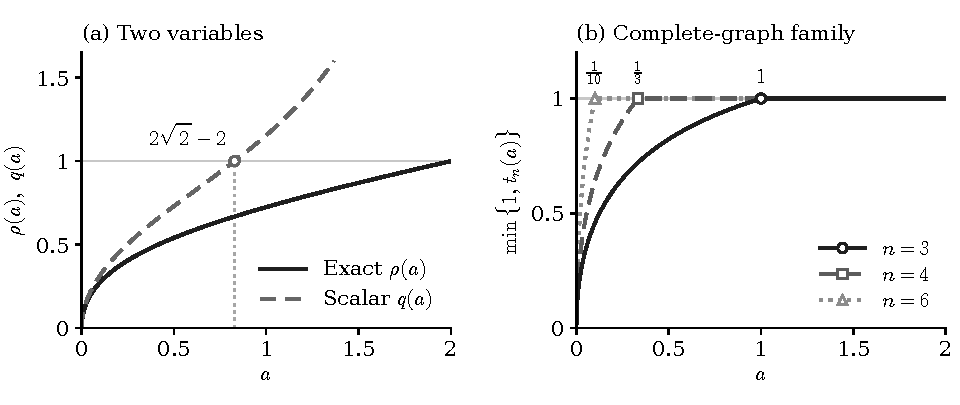
\includegraphics[width=\linewidth]{figures/rates}
\caption{Analytic Jacobi factors at $U=f^*=0$ for termwise McCormick
relaxations with exact square terms. (a) For $f=x^2+y^2+axy$, the exact
cube factor $\rho(a)$ is below one for $0<a<2$
(Proposition~\ref{prop:two-variable-rate}). The scalar quadratic-growth
bound with $\mu=1-a^2/4$ and $\tau=a/4$ gives
$q(a)=\sqrt{a/(1-a^2/4)}$; its sufficient condition $q<1$ holds only for
$a<2\sqrt2-2$ (Proposition~\ref{prop:quadratic-growth}). The scalar curve
is shown through $q=1.6$. (b) For
$f=\sum_i x_i^2+a\sum_{i<j}x_ix_j$, $n\ge3$, the exact cube factor
$\min\{1,t_n(a)\}$ reaches one at $a=2/[(n-1)(n-2)]$
(Example~\ref{ex:many-term}). Markers identify the thresholds $1$, $1/3$,
and $1/10$ for $n=3,4,6$. All objectives are strongly convex for $0<a<2$;
the plateaus denote fixed cubes at every scale. Endpoints show continuous
limits.}
\label{fig:analytic-rates}
\end{figure}

\begin{example}[The sign pattern matters]\label{ex:signed-stall}
Let $f=x_1^2+x_2^2+x_3^2+\tfrac34(x_1x_2+x_1x_3-x_2x_3)$ on $[-1,1]^3$. Its
Hessian $2I+\tfrac34A$ with $A=\left[\begin{smallmatrix}0&1&1\\1&0&-1\\1&-1&0\end{smallmatrix}\right]$
has eigenvalues $1/2,11/4,11/4$, because $(-1,1,1)$, $(0,1,-1)$, and
$(2,1,1)$ are eigenvectors of $A$ with eigenvalues $-2,1,1$. The row
condition fails in every row ($5/2>9/4$). By~\eqref{eq:cube-Q},
\[
  Q(1,\xi)=\norm{\xi}_2^2+\tfrac34\bigl(\abs{\xi_1+\xi_2}+\abs{\xi_1+\xi_3}
  +\abs{\xi_2-\xi_3}-3\bigr),
\]
and at $z=(1,-3/8,-3/8)$ the value is $41/32-18/32-24/32=-1/32$. The signed
permutations $(\xi_1,\xi_2,\xi_3)\mapsto(\xi_2,\xi_1,-\xi_3)$ and
$(\xi_1,\xi_2,\xi_3)\mapsto(\xi_3,-\xi_2,\xi_1)$ preserve the cube and
permute the three absolute values, so they preserve $Q(1,\cdot)$; they map
$z$ to points on the positive second and third faces, and $Q(1,-\xi)=Q(1,\xi)$
gives the negative faces. Theorem~\ref{thm:local-stall} applies with a strict
margin. For this objective, condition (b) of
Proposition~\ref{prop:quadratic-rows} gives the lower bound $-1/32$ on every
face value, which $z$ attains.
\end{example}

\begin{example}[The shape changes the outcome]\label{ex:shape-change}
Let $f=\sum_{i=1}^3x_i^2+\sum_{i<j}x_ix_j$, the case $a=1$, $n=3$ of
Example~\ref{ex:many-term}, for which the cube stalls with equality in the
row condition. On the thinner box $[-1/4,1/4]\times[-1,1]^2$, use the scaled
matrix $H'=\operatorname{diag}(1/4,1,1)\,H\,\operatorname{diag}(1/4,1,1)$. For
$k=1$, the witnesses $\pm e_1$ of part (a) of
Proposition~\ref{prop:quadratic-rows} give face values at most
$H'_{11}/2-S_1=1/16-1<0$. For $k=2,3$, the estimate in the proof of part (b),
which holds coordinate by coordinate, gives face values at least
$1-3/16-1/4-1/4=5/16>0$. Hence the first coordinate keeps its bounds and the
other two contract. A round changes the shape, and the face test must then
be applied to the new shape.
\end{example}

\begin{example}[Finite tangent relaxations of squares]\label{ex:finite-square}
Let $f=\sum_ix_i^2$ and relax each square $x_i^2$ by a lifted variable $y_i$
subject to the McCormick inequalities for the product $x_i\cdot x_i$, which
are the endpoint tangents $y_i\ge2\ell_ix_i-\ell_i^2$ and
$y_i\ge2u_ix_i-u_i^2$ and the secant $y_i\le(\ell_i+u_i)x_i-\ell_iu_i$; the
objective is $\sum_iy_i$. On a centered box with half-widths $h_i>0$,
$\phi_B(x)=\sum_i(2h_i\abs{x_i}-h_i^2)$, and a Jacobi round at $U=0$ gives
the exact map
\[
  h_i'=\min\Bigl\{h_i,\ \frac{1}{2h_i}\sum_jh_j^2\Bigr\}:
\]
the coordinates $j\ne i$ can be zero with $y_j=-h_j^2$, and the endpoint is
attained with these values. For $n=1$ the half-width halves each round. For
$n\ge2$ every cube is fixed, although the objective is strictly convex with
a unique minimizer; the tangent model is $Q(1,\xi)=\sum_i(2\abs{\xi_i}-1)$,
whose face values $2-n$ are nonpositive. Adding the valid rows $y_i\ge0$
changes the map to $h_i'=h_i/2$, and the exact convex squares give $\{0\}$
after one round. The rate is a property of the relaxation, not of the
problem. Section~\ref{sec:certificates} uses this finite family as its
exact reference family.
\end{example}

\subsection{Factorable functions and composite McCormick relaxations}\label{sec:local-rates-factorable}

For general smooth objectives the tangent model is computed by a recursion
over a factorable representation. A \emph{factorable representation} is a
sequence $v_1,\dots,v_m$ of functions of $x$ with $v_i=x_i$ for $i\le n$
and, for $k>n$, one of: a constant; $v_a+v_b$; $c\,v_a$ with $c\in\R$;
$v_av_b$ (with $a=b$ allowed); or $h_k(v_a)$ for a function $h_k$ of one
variable, where $a,b<k$. The objective is $f=v_m$. On a box $B$, natural
interval arithmetic gives intervals $[v_k^L(B),v_k^U(B)]$: endpoint
operations for sums and scalings, the minimum and maximum of the four
endpoint products for products, and the exact range of $h_k$ over the
interval of its argument for univariate factors. The composite McCormick
relaxation~\cite{mccormick1976-computability-of-global-solutions-to,mitsos2009-mccormick-based-relaxations-of-algorithms}
computes convex and concave relaxations $\mathrm{cv}_k\le v_k\le\mathrm{cc}_k$
on $B$ factor by factor: sums and scalings exactly (a negative scaling
exchanges the convex and concave sides); products by the rule
\begin{align*}
  \mathrm{cv}_k&=\max\bigl\{\alpha_1+\alpha_2-v_a^Lv_b^L,\ \beta_1+\beta_2-v_a^Uv_b^U\bigr\},\\
  \alpha_1&=\min\{v_b^L\mathrm{cv}_a,v_b^L\mathrm{cc}_a\},\quad
  \alpha_2=\min\{v_a^L\mathrm{cv}_b,v_a^L\mathrm{cc}_b\},\\
  \beta_1&=\min\{v_b^U\mathrm{cv}_a,v_b^U\mathrm{cc}_a\},\quad
  \beta_2=\min\{v_a^U\mathrm{cv}_b,v_a^U\mathrm{cc}_b\},
\end{align*}
and, with $\gamma_1=\max\{v_b^L\mathrm{cv}_a,v_b^L\mathrm{cc}_a\}$,
$\gamma_2=\max\{v_a^U\mathrm{cv}_b,v_a^U\mathrm{cc}_b\}$,
$\gamma_3=\max\{v_b^U\mathrm{cv}_a,v_b^U\mathrm{cc}_a\}$, and
$\gamma_4=\max\{v_a^L\mathrm{cv}_b,v_a^L\mathrm{cc}_b\}$,
\[
  \mathrm{cc}_k=\min\bigl\{\gamma_1+\gamma_2-v_a^Uv_b^L,\ \gamma_3+\gamma_4-v_a^Lv_b^U\bigr\};
\]
univariate factors are relaxed by
$\mathrm{cv}_k=h^{\mathrm{cv}}_Z(\midop\{\mathrm{cv}_a,\mathrm{cc}_a,z^{\min}\})$,
where $h^{\mathrm{cv}}_Z$ is the convex envelope of $h_k$ on
$Z=[v_a^L,v_a^U]$, $z^{\min}$ is a minimizer of $h^{\mathrm{cv}}_Z$ on $Z$, and
$\midop$ is the median of three numbers; the concave side uses the concave
envelope and a maximizer. The relaxed objective is
$\phi_B=\mathrm{cv}_m$. The \emph{clipped} variant replaces $\mathrm{cv}_k$ by
$\max\{\mathrm{cv}_k,v_k^L\}$ and $\mathrm{cc}_k$ by $\min\{\mathrm{cc}_k,v_k^U\}$
before they are used by later factors. Scott, Stuber, and Barton prove that
the clipped construction is monotone in the sense of~\eqref{eq:monotonicity}
when the natural interval of every univariate argument lies in the domain
of the corresponding scalar function and these functions are Lipschitz
there, and they note that the unclipped rule can violate
monotonicity~\cite{scott2011-generalized-mccormick-relaxations}. On small
boxes around a point at which the scalar functions are twice continuously
differentiable, these conditions hold. Validity and convexity of both
variants are standard.

The tangent model is built from first-order data. Write $v_k^*=v_k(x^*)$
and $\pi_k(\xi)=\nabla v_k(x^*)^T\xi$, and, for $t\in\R$,
$t^+=\max\{t,0\}$ and $t^-=\max\{-t,0\}$. For a shape $d$ define intervals
$[\underline\pi_k(d),\overline\pi_k(d)]$ and nonnegative functions
$E_k^{\mathrm{cv}}(d,\xi)$, $E_k^{\mathrm{cc}}(d,\xi)$, $\xi\in D(d)$, by the
following recursion.
\begin{itemize}
\item Variable $x_i$: interval $[-d_i^-,d_i^+]$, $E^{\mathrm{cv}}=E^{\mathrm{cc}}=0$.
  Constant: interval $[0,0]$, $E^{\mathrm{cv}}=E^{\mathrm{cc}}=0$.
\item Sum: intervals and both functions add.
\item Scaling $c\,v_a$: for $c\ge0$, interval $c[\underline\pi_a,\overline\pi_a]$,
  $E^{\mathrm{cv}}=cE_a^{\mathrm{cv}}$, $E^{\mathrm{cc}}=cE_a^{\mathrm{cc}}$; for
  $c<0$, interval $[c\overline\pi_a,c\underline\pi_a]$,
  $E^{\mathrm{cv}}=\abs cE_a^{\mathrm{cc}}$, $E^{\mathrm{cc}}=\abs cE_a^{\mathrm{cv}}$.
\item Product $v_av_b$: interval
  $v_b^*[\underline\pi_a,\overline\pi_a]+v_a^*[\underline\pi_b,\overline\pi_b]$
  in interval arithmetic, and
  \begin{align*}
    E^{\mathrm{cv}}&=(v_b^*)^+E_a^{\mathrm{cv}}+(v_b^*)^-E_a^{\mathrm{cc}}
      +(v_a^*)^+E_b^{\mathrm{cv}}+(v_a^*)^-E_b^{\mathrm{cc}}\\
      &\quad+\min\bigl\{(\pi_a-\underline\pi_a)(\pi_b-\underline\pi_b),\
      (\overline\pi_a-\pi_a)(\overline\pi_b-\pi_b)\bigr\},\\
    E^{\mathrm{cc}}&=(v_b^*)^+E_a^{\mathrm{cc}}+(v_b^*)^-E_a^{\mathrm{cv}}
      +(v_a^*)^+E_b^{\mathrm{cc}}+(v_a^*)^-E_b^{\mathrm{cv}}\\
      &\quad+\min\bigl\{(\overline\pi_a-\pi_a)(\pi_b-\underline\pi_b),\
      (\pi_a-\underline\pi_a)(\overline\pi_b-\pi_b)\bigr\}.
  \end{align*}
\item Univariate $h_k(v_a)$, with $h_1=h_k'(v_a^*)$, $h_2=h_k''(v_a^*)$, and
  $\sigma_a=(\pi_a-\underline\pi_a)(\overline\pi_a-\pi_a)$: interval
  $h_1[\underline\pi_a,\overline\pi_a]$, and
  \[
    E^{\mathrm{cv}}=\tfrac12h_2^-\sigma_a+h_1^+E_a^{\mathrm{cv}}+h_1^-E_a^{\mathrm{cc}},\qquad
    E^{\mathrm{cc}}=\tfrac12h_2^+\sigma_a+h_1^+E_a^{\mathrm{cc}}+h_1^-E_a^{\mathrm{cv}}.
  \]
\end{itemize}
Here $\pi_a$ stands for $\pi_a(\xi)$ and the interval endpoints for their
values at $d$. The interval $[\underline\pi_k(d),\overline\pi_k(d)]$ is
natural interval arithmetic applied to the linearized factor sequence over
$D(d)$, so it contains $\pi_k(\xi)$ for $\xi\in D(d)$; consequently every
factor of the form $\pi-\underline\pi$ or $\overline\pi-\pi$ is nonnegative
and $E_k^{\mathrm{cv}},E_k^{\mathrm{cc}}\ge0$. By induction, the interval
endpoints are continuous and positively homogeneous of degree one in $d$,
and the functions $E_k$ are continuous and positively homogeneous of degree
two in $(d,\xi)$.

\begin{theorem}[Second-order expansion of composite McCormick relaxations]\label{thm:composite-expansion}
Let $x^*\in\R^n$, and suppose that for every univariate factor
$v_k=h_k(v_a)$, the function $h_k$ is twice continuously differentiable on
an open interval containing $v_a(x^*)$. Let $\mathcal K$ be a compact set of
shapes. There is $t_{\mathcal K}>0$ such that for $0<t\le t_{\mathcal K}$ all
intervals and relaxations on $B_t=x^*+tD(d)$, $d\in\mathcal K$, are defined,
and, uniformly over $d\in\mathcal K$ and $\xi\in D(d)$, with $x_t=x^*+t\xi$,
for every factor $k$,
\begin{align}
  v_k^L(B_t)&=v_k^*+t\underline\pi_k(d)+O(t^2),\qquad
  v_k^U(B_t)=v_k^*+t\overline\pi_k(d)+O(t^2),\label{eq:expansion-interval}\\
  \mathrm{cv}_k(x_t)&=v_k(x_t)-t^2E_k^{\mathrm{cv}}(d,\xi)+o(t^2),\qquad
  \mathrm{cc}_k(x_t)=v_k(x_t)+t^2E_k^{\mathrm{cc}}(d,\xi)+o(t^2),\label{eq:expansion-relaxation}\\
  v_k^L(B_t)&-\mathrm{cv}_k(x_t)\le o(t^2),\qquad
  \mathrm{cc}_k(x_t)-v_k^U(B_t)\le o(t^2),\label{eq:expansion-dominance}
\end{align}
where the relaxations are those built on $B_t$. If each $h_k''$ is
Lipschitz near $v_a(x^*)$, every $o(t^2)$ can be replaced by $O(t^3)$. The
clipped relaxations have the same expansions. Consequently,
\[
  \phi_{B_t}(x_t)=f(x^*)+t\nabla f(x^*)^T\xi+t^2Q(d,\xi)+o(t^2),\qquad
  Q(d,\xi)=\tfrac12\xi^T\nabla^2f(x^*)\xi-E_m^{\mathrm{cv}}(d,\xi),
\]
uniformly on $\mathcal K$, and $Q$ is continuous. At a minimizer with
$\nabla f(x^*)=0$ at which the relaxations are monotone, for example in
the clipped construction, Assumption~\ref{ass:tangent} holds.
\end{theorem}

The proof is in Appendix~\ref{sec:local-proofs-composite}. Its main step
concerns univariate factors: the median rule can clip the argument of the
envelope at an endpoint of its interval, and~\eqref{eq:expansion-dominance}
shows that this clipping does not change the second-order term. The
expansion covers zero factor values, critical points $h_k'(v_a^*)=0$,
inflection points $h_k''(v_a^*)=0$, first-order intervals of zero width,
and shapes with zero components. The box $B_0$ plays no role, so the
theorem also applies at minimizers on the boundary of $B_0$, with shapes
restricted to the admissible ones; this is used in
Section~\ref{sec:local-rates-boundary}. The smoothness hypothesis concerns
each scalar factor at its own argument, and smoothness of $f$ does not
replace it. For example, $f(x)=\abs x-\abs x+x^2=x^2$, with the square kept
exact, has on $[-t,t]$ the composite relaxation $x^2+\abs x-t$, with or
without clipping: the concave envelope of $\abs x$ is the constant $t$, and
the subtraction uses it. The gap at $x^*=0$ is $t$, of first order. The
direct relaxation of $\abs x$ itself is exact, so nonsmoothness alone does
not force such an error; the theorem simply does not apply at a kink. At a
nonzero argument, $\abs{\cdot}$ is linear nearby and the theorem applies.

Two consequences are worth stating. First, for quadratic objectives with
the squares represented as univariate factors and the products of distinct
variables as products, $E_m^{\mathrm{cv}}$ is the McCormick gap and
Theorem~\ref{thm:composite-expansion} reproduces~\eqref{eq:quadratic-Q}.
Representing $x_i^2$ instead as the product $x_i\cdot x_i$ gives, at
$x_i^*=0$, the gap $\min\{(\xi_i+d_i^-)^2,(d_i^+-\xi_i)^2\}$ and the model
$2\abs{\xi_i}-1$ on the unit interval, which is the finite tangent
relaxation of Example~\ref{ex:finite-square}. The tangent model therefore
depends on the factorable representation as well as on the rules. Second,
since $E_m^{\mathrm{cv}}$ is bounded on compact sets, the theorem gives
$\phi_B\ge f-Cw(B)^2$ on small boxes containing $x^*$. This recovers, near
$x^*$, the second-order pointwise convergence of McCormick
relaxations~\cite{bompadre2012-convergence-rate-of-mccormick-relaxations}; the theorem
adds the limit of the scaled gap as a function of the box shape and of the
position in the box, which is what the tangent map needs.

Solvers usually relax lifted reformulations with an auxiliary variable per
factor. For quadratic problems whose auxiliary variables occur only in the
objective, minimizing over the auxiliaries decouples the terms. With exact
convex squares and McCormick envelopes for the products of distinct
variables, this yields the termwise relaxation, so~\eqref{eq:quadratic-Q}
applies exactly; with finite tangent relaxations of the squares it yields
the model of Example~\ref{ex:finite-square}. When
auxiliary variables also occur in constraints, or when cuts are added,
Theorem~\ref{thm:composite-expansion} does not apply, and
Assumption~\ref{ass:tangent} is a hypothesis to be verified for the
construction at hand.

\subsection{Minimizers on the boundary of the box}\label{sec:local-rates-boundary}

At a minimizer on the boundary of $B_0$ with nonzero derivatives across the
active faces, the first-order term dominates in the active coordinates.
Let $x^*$ be a global minimizer with $x_i^*=\ell_i^0$ for $i$ in an active
set $A$ and $\ell_i^0<x_i^*<u_i^0$ for $i$ in the free set $F$; active upper
bounds reduce to this case by reflecting the coordinate. We assume that $A$ and $F$ are both nonempty; the case $F=\emptyset$ is
discussed after Theorem~\ref{thm:boundary}. Let $g\in\R^n$ satisfy $g_i>0$
for $i\in A$ and $g_i=0$ for $i\in F$. For a differentiable objective with
$g=\nabla f(x^*)$ and no constraints other than the bounds, these are the
first-order optimality conditions with strict complementarity; with other
constraints, $g$ is the first-order coefficient of the projected
relaxation in Assumption~\ref{ass:boundary} below. Admissible shapes form the closed cone
$\mathcal S=\{d\ge0:d_i^-=0\text{ for }i\in A\}$; every box $B$ with
$x^*\in B\subseteq B_0$ equals $x^*+tD(d)$ with $d\in\mathcal S$. Write
$w_i(B)=u_i-\ell_i$ for the width of coordinate $i$.

\begin{assumption}[Boundary tangent model]\label{ass:boundary}
There is a continuous function $Q(d,\xi)$ on
$\{(d,\xi):d\in\mathcal S,\ \xi\in D(d)\}$ such that for every compact
$\mathcal K\subseteq\mathcal S$ the comparison boxes belong to $\mathfrak B$
for small $t$ and
\[
  \varrho_{\mathcal K}(t)=\sup_{d\in\mathcal K,\ \xi\in D(d)}
  \frac{\bigl|\phi_{x^*+tD(d)}(x^*+t\xi)-f^*-tg^T\xi-t^2Q(d,\xi)\bigr|}{t^2}
  \longrightarrow0.
\]
\end{assumption}

The essential point is that $\mathcal K$ may contain shapes whose active
components are zero or small. Theorem~\ref{thm:composite-expansion}
supplies Assumption~\ref{ass:boundary} for clipped composite McCormick
relaxations with $g=\nabla f(x^*)$. For a free shape $d_F$ let $\iota(d_F)$ be
the shape with free part $d_F$ and zero active components, define $\iota$
on points in the same way, and set
\[
  Q^F(d_F,\xi_F)=Q(\iota(d_F),\iota(\xi_F)),\qquad
  G^F(d_F)=-\min_{\xi_F\in D_F(d_F)}Q^F(d_F,\xi_F)\ge0.
\]
The reduced tangent map $\Phi^F_c$ and its factor $r^*(\Phi^F)$ are defined
from $Q^F$ as in Section~\ref{sec:local-rates-tangent}. For the boundary
theorem fix a free shape $u_F\gg0$ and a bound $M\ge0$ on the initial
active components, and let
\[
  G_0=G^F(u_F),\qquad
  G_M=-\min\{Q(d,\xi):d\in\mathcal S,\ d_F=u_F,\ d_A^+\le M,\ \xi\in D(d)\},
  \qquad g_{\min}=\min_{i\in A}g_i.
\]
Since $\iota(u_F)$ is admissible, $0\le G_0\le G_M$.

\begin{lemma}[One round near a boundary minimizer]\label{lem:boundary-step}
Let Assumption~\ref{ass:boundary} hold, let $\delta>0$, and let $\mathcal K_F$
be a compact set of free shapes. There are $\bar t,\bar\sigma>0$ such that
for every box $B=x^*+tD(d)$ with $d\in\mathcal S$, $d_F\in\mathcal K_F$,
$\max_{i\in A}d_i^+\le\bar\sigma$, and $t\le\bar t$, and every $\epsilon\ge0$:
\begin{enumerate}[label=(\roman*)]
\item if $\epsilon\le\delta t^2/2$, the free part of $T_U(B)$ lies in
  $x_F^*+tD_F(\Phi^F_\delta(d_F))$;
\item $x^*+t\iota(\xi_F)\in K_U(B)$ for every $\xi_F\in D_F(d_F)$ with
  $Q^F(d_F,\xi_F)\le-\delta$;
\item $w_i(T_U(B))\le\bigl(\epsilon+(G^F(d_F)+\delta/2)t^2\bigr)/g_i$ for
  $i\in A$;
\item $w_i(T_U(B))\ge\min\bigl\{td_i^+,\ \bigl(\epsilon+(G^F(d_F)-\delta/2)t^2\bigr)/g_i\bigr\}$
  for $i\in A$.
\end{enumerate}
\end{lemma}

Parts (i) and (ii) say that in scaled coordinates the free part of one
round lies between the hulls of the sublevel sets of $Q^F$ at levels
$-\delta$ and $\delta$. Parts (iii) and (iv) show that the bound on the active
widths is sharp to first order, since $\delta$ is arbitrary. The proof is
in Appendix~\ref{sec:local-proofs-boundary}.

\begin{theorem}[Boundary minimizers]\label{thm:boundary}
Let Assumption~\ref{ass:boundary} hold, and let $u_F\gg0$, $\delta>0$, and
$\lambda\in(0,1)$ satisfy $\Phi^F_\delta(u_F)\le\lambda u_F$. Let $M\ge0$.
There is $\bar t>0$ with the following property. Let the start box satisfy
$x^*\in B_0\subseteq x^*+t_0D(d^0)$ with an admissible shape
$d^0\in\mathcal S$, $d^0_F=u_F$, $\max_{i\in A}(d^0)_i^+\le M$, and
$0<t_0\le\bar t$, and consider Jacobi iterates, or complete sequential
rounds, from $B_0$ at cutoff $U=f^*+\epsilon$. Put $t_k=\lambda^{k-1}t_0$ for $k\ge1$, and let
$N=\min\{k\ge1:t_k^2<2\epsilon/\delta\}$, with $N=\infty$ if $\epsilon=0$.
\begin{enumerate}[label=(\alph*)]
\item For $1\le k\le N$, the free part of $B_k$ lies in
  $x_F^*+t_kD_F(u_F)$.
\item $w_i(B_1)\le\bigl(\epsilon+(G_M+\delta/4)t_0^2\bigr)/g_i$ for $i\in A$. If
  $N\ge2$, then for $1\le k\le N$ and $i\in A$,
  \[
    w_i(B_{k+1})\le\bigl(\epsilon+(G_0+\eta_k)t_k^2\bigr)/g_i,
  \]
  with $0\le\eta_k\le\delta/2$, and $\eta_k\to0$ as $t_k\to0$.
\item If $\epsilon=0$, then $B_\infty=\{x^*\}$, the free widths are
  $O(\lambda^k)$ by (a), and $w_i(B_{k+1})\le(G_0/g_i+o(1))\,t_k^2$. If $\epsilon>0$, the free part of
  $B_\infty$ lies in $x_F^*+\sqrt{2\epsilon/\delta}\,D_F(u_F)$ and
  $w_i(B_\infty)\le(2+2G_M/\delta)\,\epsilon/g_i$ for $i\in A$.
\end{enumerate}
Every $\lambda>r^*(\Phi^F)$ admits such $u_F$ and $\delta$.
\end{theorem}

The free coordinates thus obey the upper bounds of the interior theory,
with the reduced map $\Phi^F$ and a floor of order at most $\sqrt\epsilon$,
while the active widths are at most of order $\epsilon$ plus the square of
the free scale $t_k$. The statement bounds the free parts and the active
widths by the common geometric scale $t_k$; it does not assert that the
actual free gauge contracts in every round. It need not: for $f=x+y^2$ on
$x\ge0$ with the valid monotone family $\phi_B=f-h^2$, where $h$ is the
upper extent of $B$ in $x$, a Jacobi round at zero cutoff maps the active
extent $h$ to $\min\{h,h^2\}$ and the free radius $r$ to $\min\{r,h\}$, so from
$[0,t_0]\times[-t_0^3,t_0^3]$ with $0<t_0<1$ the free radius does not move in
the first two rounds. The proof is in Appendix~\ref{sec:local-proofs-boundary}. If
$g_i=0$ for some active $i$, that coordinate has no first-order term. It
can be treated as a free coordinate restricted to shapes with $d_i^-=0$:
the same proof applies to the enlarged free set, provided the contraction
hypothesis $\Phi^F_\delta(u_F)\le\lambda u_F$ is verified on this one-sided
cone of shapes. If all coordinates are active ($F=\emptyset$) with
$g_i>0$, Proposition~\ref{prop:sharp-growth} applies on small boxes: at zero
cutoff slack the convergence is quadratic, and at a positive slack the
widths satisfy the forced recurrence of that proposition and end at most
$4\epsilon/\kappa$.

The refined estimate in (b) requires $N\ge2$. If the initial scale already
lies below the cutoff floor, the active components of $B_1$ need not be
small relative to $t_1$, and the refined constant can fail. For
$f(x,y)=x-x^2+y^2$ on $[0,1/4]\times[-1/4,1/4]$, keep $y^2$ exact and use the
secant $-hx$ of $-x^2$ on $[0,h]$. On $B=[0,h]\times[-r,r]$ the relaxation is
$(1-h)x+y^2$; the expansion is exact with $g=(1,0)$ and
$Q(d,\xi)=-d_x^+\xi_x+\xi_y^2$, so $G_0=0$, and $u_F=1$, $\delta=1/4$,
$\lambda=3/4$, $M=1$ satisfy the hypotheses. Start from
$[0,w_0]\times[-w_0,w_0]$ with $\epsilon=w_0/2$ and $w_0$ small. Then $N=1$,
the free bounds do not move in the first two rounds, and the active widths
are $h_1=\epsilon/(1-w_0)$ and $h_2=\epsilon/(1-h_1)$. Hence
$(h_2-\epsilon)/w_0^2=1/(4-6w_0)>1/4$, whereas the refined estimate would give
at most $\delta/2=1/8$.

\begin{example}[An exact boundary example]\label{ex:boundary}
Let $f=x_1+x_2^2+x_3^2+ax_2x_3$ with $0<a<2$ on $[0,1]\times[-1,1]^2$, with
exact squares and the McCormick underestimator of $x_2x_3$. The minimizer
is $0$, with $A=\{1\}$, $g_1=1$, and $G_0=a$. On $B=[0,h]\times[-s,s]^2$ the
relaxation is $x_1+\psi_s(x_2,x_3)$ with
$\psi_s=x_2^2+x_3^2+as\abs{x_2+x_3}-as^2$, whose minimum is $-as^2$. A Jacobi
round at cutoff $\epsilon$ therefore maps $(h,s)$ to
\[
  \bigl(\min\{h,\ \epsilon+as^2\},\ g(s)\bigr),
\]
with $g$ as in Proposition~\ref{prop:two-variable-cutoff-floor}: the
largest free extent is attained with $x_1=0$, and the largest active extent
with $(x_2,x_3)=0$. For $\epsilon=0$ the free half-width is $\rho(a)^ks_0$ and
the active width is $a\rho(a)^{2k-2}s_0^2$ once it falls below $h_0$. For
$\epsilon>0$ and $s_0\ge h_\epsilon$, the free half-width decreases to
$h_\epsilon$ and the active width to
$\min\{h_0,\ \epsilon(1+a/(1-a^2/4))\}$: a free floor of order $\sqrt\epsilon$
and an active floor of order $\epsilon$. For $a=1$ the limit widths are
$2h_\epsilon=(4/\sqrt3)\sqrt\epsilon\approx2.309\sqrt\epsilon$ and, for large
$h_0$, $7\epsilon/3$.
\end{example}

\subsection{The relaxation gap after tightening, and stopping}\label{sec:local-rates-consequences}

The width of the limit box matters because it controls the relaxation gap
that remains after tightening.

\begin{corollary}[Gap after tightening]\label{cor:local-gap}
Under the hypotheses of Theorem~\ref{thm:tangent-contraction}(b), let
\[
  G=-\min_{\xi\in D(u)}Q(u,\xi)\ge0.
\]
If $\epsilon>0$ and $\sqrt{2\epsilon/\delta}\le\bar t$, then
\[
  f^*-L(B_\infty)\le\Bigl(\frac{2G}{\delta}+1\Bigr)\epsilon,
\]
and $f^*-L(B_\infty)\le(2G/\delta)\epsilon+o(\epsilon)$ as $\epsilon\downarrow0$;
for $\epsilon=0$, $L(B_\infty)=f^*$. Under the hypotheses of
Proposition~\ref{prop:sharp-growth}, once an iterate has width at most
$\kappa/(4\tau)$ (any iterate if $\tau=0$),
$f^*-L(B_\infty)\le16\tau\epsilon^2/\kappa^2$.
\end{corollary}

\begin{proof}
Let $t_\epsilon=\sqrt{2\epsilon/\delta}$ and $C=x^*+t_\epsilon D(u)$. By
Theorem~\ref{thm:tangent-contraction}, $B_\infty\subseteq C$, so $L(B_\infty)\ge L(C)$.
For $x=x^*+t_\epsilon\xi\in C$,
$\phi_C(x)\ge f^*+t_\epsilon^2Q(u,\xi)-\varrho_{\{u\}}(t_\epsilon)t_\epsilon^2
\ge f^*-Gt_\epsilon^2-\varrho_{\{u\}}(t_\epsilon)t_\epsilon^2$. Since
$\varrho_{\{u\}}(t_\epsilon)\le\delta/2$, this gives the first bound, and since
$\varrho_{\{u\}}(t_\epsilon)\to0$, the second. For $\epsilon=0$,
$B_\infty=\{x^*\}$ lies in every comparison box, so the same estimate with
$t\downarrow0$ gives $L(B_\infty)\ge f^*$, and validity at $x^*$ gives equality.
In the sharp case,~\eqref{eq:sharp-growth} gives $L(B)\ge f^*-\tau w(B)^2$
for boxes containing $x^*$, and $w(B_\infty)\le4\epsilon/\kappa$.
\end{proof}

Under the contraction hypotheses, the gap left after tightening to the
limit is at most proportional to the incumbent's suboptimality $\epsilon$;
for the model problem it equals $a\epsilon/(1-a^2/4)$
(Proposition~\ref{prop:two-variable-cutoff-floor}). Together with the
$O(\sqrt\epsilon)$ bound on the width, this has several consequences for
deciding when to tighten.

\paragraph{Rounds to the cutoff floor.} Under the hypotheses of
Theorem~\ref{thm:tangent-contraction}, the gauge falls at least by the
factor $\lambda$ per round until it is below $\sqrt{2\epsilon/\delta}$.
For $\epsilon>0$, zero rounds suffice when the starting gauge satisfies
$t_0\le\sqrt{2\epsilon/\delta}$. Otherwise at most
$\bigl\lceil\log\bigl(t_0\sqrt{\delta/(2\epsilon)}\bigr)/\log(1/\lambda)\bigr\rceil$
rounds bring the iterates inside $x^*+\sqrt{2\epsilon/\delta}\,D(u)$, which
contains the limit; further rounds change the box only inside this region
and change the gap by at most the $O(\epsilon)$ bound above. This bound on
the number of rounds grows only logarithmically as $\epsilon$ decreases.

\paragraph{When to repeat after an incumbent improves.} Lowering the
cutoff slack from $\epsilon$ to $\epsilon'$ lowers the bounds on the limit
width by the factor $\sqrt{\epsilon'/\epsilon}$ and the bounds on the remaining
gap by the factor $\epsilon'/\epsilon$; in the model problem the limit itself
shrinks by exactly these factors. This is the local reason to repeat
tightening after an incumbent improves, and the reason why a cutoff far
above $f^*$ limits the value of any number of rounds. In the stall regime
of Theorem~\ref{thm:local-stall}, by contrast, no improvement of the
incumbent removes the fixed boxes around $x^*$.

\paragraph{What observed ratios show.} The successive width ratios of an
iteration are a natural signal for stopping, and they estimate the
contraction rate in favorable cases. They are not a certificate. From boxes
that are not eigenvectors, early ratios can lie far below the asymptotic
rate (the example after Proposition~\ref{prop:rectangle-map});
near a positive floor the ratios tend to one while the distance to the
limit contracts quickly (Proposition~\ref{prop:two-variable-cutoff-floor}(d));
a ratio near one can thus indicate a rate near one, the approach to a floor,
or a stall. Example~\ref{ex:critical-scalar} has ratios tending to one and still
converges to a point, sublinearly. Proposition~\ref{prop:history} gives valid
monotone relaxation families whose iterations share arbitrarily long
histories and then either stall or contract to a point. Observed ratios
therefore support stopping heuristics, not guarantees.

\paragraph{Which regimes admit finite certificates.} In the stall regime,
the witnesses of Theorem~\ref{thm:local-stall} are finitely many points
whose coordinate hull is a fixed box at every small scale; they are a
certificate of the kind developed in Section~\ref{sec:certificates}. In the
contracting regime with $\epsilon>0$, the limit box is a fixed box of width
$O(\sqrt\epsilon)$ under~\eqref{eq:closed-family}, and $2n$ points
attaining its faces certify it, as in
Proposition~\ref{prop:two-variable-cutoff-floor}(b). In the contracting
regime with $\epsilon=0$, the only fixed box containing $x^*$ in a small
neighborhood is $\{x^*\}$; no box of positive width can certify that the
remaining movement is zero. An iterate that reaches $\{x^*\}$ can be
certified as fixed. If convergence is only asymptotic, as in the model
problem, a bound on the remaining movement, such as the residual certificate
of Section~\ref{sec:residual}, justifies a tolerance stop. When the optimal
incumbent lies in the current box, its protected singleton
(Corollary~\ref{cor:original-points}) already bounds the remaining movement,
and the bound is exact if the iterates converge to it.
These cases do not exhaust the possibilities:
Example~\ref{ex:critical-scalar} has no fixed box of positive width and no
geometric contraction.

\paragraph{Symmetry and spread minimizers.} By Lemma~\ref{lem:sublevel-hull},
several global minimizers keep their hull in every iterate, whatever the
local rates. Tightening at the root of a symmetric model cannot converge to a single
point until branching separates the minimizers. At a node that contains a
single minimizer, the conclusions of this section apply when their
hypotheses hold: a tangent model, monotonicity on the comparison boxes, a
contraction shape, and a start box in the local region. A single minimizer
does not supply them; Example~\ref{ex:many-term} has a unique minimizer and
stalls.

\section{Finite witness certificates}\label{sec:certificates}

Before paying for another OBBT round, a solver would like to know how much
that round, or all remaining rounds, can still change. This section bounds
the change from above with finite sets of points that are feasible for the
relaxation. The bounds concern a specified tightening procedure and a
specified relaxation family. They are not new variable bounds, and they do
not by themselves predict solving time. Three statements must be kept apart.
\begin{enumerate}
\item A point feasible for the current relaxation bounds the improvement
  of one frozen round (Section~\ref{sec:cert-current}).
\item Points feasible for the relaxation rebuilt on an inner box $P$ bound
  the improvement of every later round, directional update, and compatible
  cutoff, provided the box being tightened contains $P$
  (Sections~\ref{sec:cert-protected}--\ref{sec:cert-scope}).
\item A residual and a verified sensitivity bound limit the remaining
  movement of an exact iteration (Section~\ref{sec:residual}).
\end{enumerate}
Statement~1 is the feasibility filtering of Gleixner et
al.~\cite{gleixner2017-three-enhancements-for-optimization-based}.
Statement~2 rests on the persistence of fixed boxes
(Lemma~\ref{lem:fixed-persist}), the order argument behind monotone
domain-reduction iterations
\cite{tarski1955fixpoint,caprara2010-global-optimization-problems-and-domain}.
The OBBT-specific content of this section is a finite certificate for a
fixed box, checked exactly on the rebuilt relaxation; a description of the
operations it covers and of those it does not; its exactness at the limit
of the iteration; and the difference between finding such a certificate
and checking it.

\subsection{Witnesses and lifted reuse}\label{sec:cert-setting}

We use the setting of Section~\ref{sec:foundations}: the relaxation family
is valid~\eqref{eq:validity} and monotone~\eqref{eq:monotonicity}, each
$\phi_B$ is lower semicontinuous, and a lifted family has compact sets
$R(B)$ and a continuous objective $v$. The cutoff sets $K_U(B)$, the
operator $T_U$, the relaxation bound $L(B)$, fixed boxes, and the Jacobi,
directional, sequential, and selective update schemes are as defined
there.

A \emph{lifted witness} on a box $P$ at cutoff $U$ is a complete lifted
vector $z\in R(P)$, including every auxiliary coordinate, that satisfies
every row of the relaxation rebuilt on $P$ and has $v(z)\le U$. By
\eqref{eq:projected}, its projection $\pi(z)$ satisfies
$\phi_P(\pi(z))\le v(z)\le U$, so $\pi(z)\in K_U(P)$. This direction needs
no attainment premise; a checked lifted witness always certifies a
projected one.

Two order properties play different roles below. All coordinate and
objective-value ceilings in this section need only the monotonicity
\eqref{eq:monotonicity} of the projected objectives. Lifted monotonicity,
$R(B')\subseteq R(B)$ for $B'\subseteq B$ with a common objective, is
needed for a different use: to treat a stored lifted point $z\in R(P)$
itself, with its stored value $v(z)$, as a feasible point of the linear
program on a box $B\supseteq P$. Such reuse lets a solver screen a later
frozen round, mix witnesses for a new cutoff (Section~\ref{sec:cutoff}),
or warm-start a later solve without recomputing auxiliary coordinates.
Under monotonicity alone, $\phi_B(\pi(z))\le\phi_P(\pi(z))\le v(z)$ still
holds, but a feasible lift on $B$ must be recomputed.

\paragraph{The reference family.}
Several examples use the lifted linear family with McCormick product rows
listed in Section~\ref{sec:foundations}. Its rows are of three kinds. Fixed rows
$Gz\le g$ do not depend on the box; they include the original linear
constraints, quadratic constraints written linearly in lifted product
variables, and valid inequalities such as $y_k\ge0$ for a lifted square.
Bound rows are $\ell\le x\le u$. For each lifted variable $y_k$ standing
for a product $x_ix_j$, with $i=j$ allowed, the four McCormick
inequalities~\cite{mccormick1976-computability-of-global-solutions-to} on
$B=[\ell,u]$ can be written as
\begin{equation}\label{eq:mccormick-gap}
\begin{aligned}
 y_k-x_ix_j&\ge-\min\{(x_i-\ell_i)(x_j-\ell_j),\,(u_i-x_i)(u_j-x_j)\},\\
 y_k-x_ix_j&\le\min\{(u_i-x_i)(x_j-\ell_j),\,(x_i-\ell_i)(u_j-x_j)\}.
\end{aligned}
\end{equation}
After the product $x_ix_j$ cancels, each of the four inequalities is
affine in $(x,y_k)$. For example, the first reads
$y_k\ge\ell_jx_i+\ell_ix_j-\ell_i\ell_j$. When $i=j$ the two upper
inequalities coincide, and the rows are the tangents of $x_i^2$ at both
endpoints together with the secant. This is a finite linear relaxation of
the square, not its convex epigraph. The objective is a fixed affine
function $v(z)=c^Tz+c_0$.

\begin{lemma}[The reference family]\label{lem:reference-family}
The reference family is lifted monotone with a common objective, and hence
monotone. Each $R(B)$ is a polytope. If the fixed rows are valid for the
original problem and $v$ evaluated at the graph lift $y_k=x_ix_j$ equals
$f(x)$, the family is valid.
\end{lemma}
\begin{proof}
Let $B'=[\ell',u']\subseteq B=[\ell,u]$ and $x\in B'$. Then
$0\le x_i-\ell'_i\le x_i-\ell_i$ and $0\le u'_i-x_i\le u_i-x_i$ for every
$i$. Each product in~\eqref{eq:mccormick-gap} multiplies two such
nonnegative distances, so its value on $B'$ is at most its value on $B$.
Consequently each lower bound on $y_k-x_ix_j$ on $B'$ is at least the
corresponding lower bound on $B$, and each upper bound is at most the
corresponding upper bound. Fixed rows and the objective do not depend on
the box, and bound rows on $B'$ imply those on $B$. Thus
$R(B')\subseteq R(B)$. The set $R(B)$ is a polyhedron; it is bounded
because $x\in B$ and each $y_k$ lies between affine functions of $x$.
At the graph lift the middle terms in~\eqref{eq:mccormick-gap} vanish,
and all bounds have the correct sign because every distance is
nonnegative on $B$. Together with valid fixed rows, this puts the graph
lift of each $x\in X\cap B$ in $R(B)$, so $\phi_B(x)\le f(x)$.
\end{proof}

\begin{example}[Monotonicity without lifted monotonicity]\label{ex:lambda}
Relax $s=x^2$ on a box $[\ell,u]$ by the convex-combination formulation
common in piecewise-linear relaxations: auxiliary weights
$\lambda_0,\lambda_1\ge0$ with $\lambda_0+\lambda_1=1$ and
$x=\lambda_0\ell+\lambda_1u$, the secant row
$s\le\lambda_0\ell^2+\lambda_1u^2$, the two endpoint tangents, and the
objective $v=s$. In every case
$\lambda_0\ell^2+\lambda_1u^2=(\ell+u)x-\ell u$, and for $\ell<u$ the
weights are determined by $x$. The projection onto
$(x,s)$ is therefore the square relaxation of the reference family, and
since the objective depends only on $s$, the projected objectives are
those of that family, which are monotone by
Lemma~\ref{lem:reference-family}. Lifted monotonicity fails: on
$P=[0,1/2]$ the point $x=1/2$ has weights $(0,1)$, while on $B=[0,1]$ it
requires $(1/2,1/2)$. A stored lifted witness for $P$ is not a feasible
point of the relaxation on $B$, although its projection remains in every
projected set that the certificates below use.
\end{example}

\subsection{The current frozen round}\label{sec:cert-current}

\begin{proposition}[Current-round ceilings]\label{prop:current-round}
Let $B=[\ell,u]$, let $W$ be a nonempty finite subset of $K_U(B)$, and
write $T_U(B)=[\ell',u']$. For every coordinate $i$,
\begin{equation}\label{eq:current-ceilings}
 0\le\ell'_i-\ell_i\le\min_{x\in W}x_i-\ell_i,\qquad
 0\le u_i-u'_i\le u_i-\max_{x\in W}x_i.
\end{equation}
\end{proposition}
\begin{proof}
The coordinate minimum over $K_U(B)$ is at most the minimum over its
subset $W$, and the maximum is at least the maximum over $W$. Since
$K_U(B)\subseteq B$, the new endpoints lie in $[\ell_i,u_i]$.
\end{proof}

A witness attaining an endpoint proves that this direction cannot move in
the present round, and one point can screen several directions. The
ceilings bound possible benefit; a witness coordinate is not a valid new
bound. Points produced by earlier support solves of the same round, or
an optimal solution of the relaxation itself, are typical witnesses.
Checking $k$ lifted points against $N$ nonzero row coefficients costs
$O(kN)$ arithmetic operations. Finding good points can cost as much as the
round itself. A ceiling on coordinate movement also says nothing about
side products of a support solve, such as dual information used for
Lagrangian variable
bounds~\cite{gleixner2017-three-enhancements-for-optimization-based}.

The ceiling~\eqref{eq:current-ceilings} concerns the frozen relaxation
on $B$. After rebuilding on a smaller box, the same point may be
infeasible, and later rounds may move much further.

\begin{example}[A frozen witness does not bound later rounds]\label{ex:halving}
Minimize $f(x)=x^2$ over $B_0=[-r_0,r_0]$, $r_0>0$, with the square
relaxation of the reference family, objective $v=s$, and the cutoff $U=0$
given by the incumbent $x=0$; this is the case $n=1$ of
Example~\ref{ex:finite-square}. On $[-r,r]$ the rows are $s\ge2r|x|-r^2$
(the two tangents) and $s\le r^2$ (the secant). With $s\le0$ they give
$|x|\le r/2$, and every such $x$ has the lift $s=0$. Hence
$T_0([-r,r])=[-r/2,r/2]$, and the exact Jacobi iterates are
$B_k=[-2^{-k}r_0,2^{-k}r_0]$. In the first round the witness $(r_0/2,0)$
bounds the decrease of the upper endpoint by $r_0/2$, which is exact for
that round. After rebuilding on $[-r_0/2,r_0/2]$, the new upper tangent
requires $s\ge r_0x-r_0^2/4=r_0^2/4>0$ at $x=r_0/2$, so the witness is
excluded. The total decrease over all rounds is $r_0$.
\end{example}

\subsection{Protected boxes}\label{sec:cert-protected}

A witness remains useful in all later rounds if it is feasible for the
relaxation built on a box that every later box contains. The following
definitions make this precise and describe the operations that preserve
such a box.

\begin{definition}[Relaxation-sound step]
A box $C'$ is obtained from a box $C$ by a relaxation-sound step at
cutoff $U'$ if $T_{U'}(C)\subseteq C'\subseteq C$.
\end{definition}

A Jacobi round is a relaxation-sound step with $C'=T_{U'}(C)$. So is a
directional update, and so is the simultaneous update of any selected set
of endpoints on one frozen relaxation. Sequential and selective rounds
are sequences of such steps. Conservative versions, which move each
selected endpoint at most to its exact support, are also relaxation-sound.
This includes OBBT whose endpoint bounds are proved by safe dual bounds
evaluated with directed rounding (Proposition~\ref{prop:dual-residual}).
Rounding an approximate optimum outward alone does not prove such a bound.
The identity step is relaxation-sound.

\begin{definition}[Witness pool and protected box]
Let $P=[a,b]$ be a nonempty box. A \emph{witness pool} for $P$ is a
finite set $W\subseteq K_U(P)$ with $\hull W=P$; that is, for every
coordinate $i$ some $x\in W$ has $x_i=a_i$ and some $x'\in W$ has
$x'_i=b_i$. The \emph{threshold} of $W$ is
$U_W=\max_{x\in W}\phi_P(x)\le U$. A box with a witness pool is
\emph{protected} at every cutoff $U'\ge U_W$.
\end{definition}

The definition evaluates $\phi_P$, the relaxation \emph{rebuilt on $P$},
not the relaxation on a larger current box. In lifted form, a pool
consists of lifted witnesses on $P$; their stored values $v(z)$ bound the
threshold from above. At most $2n$ points are needed, one for each
endpoint, and fewer suffice when one point attains several endpoints. A
protected box is a fixed box; the word \emph{protected} refers to the
finite certificate and its threshold.

\begin{theorem}[Protection]\label{thm:protected}
Let $W$ be a witness pool for $P=[a,b]$ with threshold $U_W$. Let
$C_0\supseteq P$ be a box in $B_0$, and for $k\ge0$ let $C_{k+1}$ be
obtained from $C_k$ by a relaxation-sound step at a cutoff $U_k\ge U_W$.
Then:
\begin{enumerate}[label=(\alph*)]
\item $T_{U'}(P)=P$ for every $U'\ge U_W$;
\item $P\subseteq C_k$ and $W\subseteq K_{U_k}(C_k)$ for every $k$; in
  particular no step proves $C_k$ infeasible at its cutoff;
\item writing $C_k=[\ell^k,u^k]$, for every $i$ and $k$,
\begin{equation}\label{eq:protected-ceilings}
 0\le\ell^k_i-\ell^0_i\le a_i-\ell^0_i,\qquad
 0\le u^0_i-u^k_i\le u^0_i-b_i.
\end{equation}
\end{enumerate}
\end{theorem}
\begin{proof}
(a) For $U'\ge U_W$, $W\subseteq K_{U_W}(P)\subseteq K_{U'}(P)$, so
$P=\hull W\subseteq T_{U'}(P)\subseteq P$.
(b) By (a), $P$ is a fixed box of $T_{U_W}$. If $P\subseteq C_k$, then
Lemma~\ref{lem:fixed-persist} gives $P\subseteq T_{U_k}(C_k)\subseteq
C_{k+1}$, and induction gives $P\subseteq C_k$ for every $k$.
Lemma~\ref{lem:order} gives $W\subseteq K_{U_W}(P)\subseteq
K_{U_k}(C_k)$.
(c) The inequalities restate $P\subseteq C_k\subseteq C_0$.
\end{proof}

The theorem needs no continuity, convergence, or fairness in the choice of
directions; the steps may mix Jacobi rounds and directional updates and
may use different cutoffs above $U_W$. The witnesses need not be
feasible for the original problem, and none of them needs to be an
optimal solution of a support problem. The essential requirement is
feasibility in the relaxation rebuilt on $P$. In
Example~\ref{ex:halving} the first-round witnesses are feasible on $B_0$
but not on their own hull, and indeed that hull is not retained.

A protected box limits what the specified OBBT procedure can remove. It
is not a domain reduction and never replaces the search domain. For
instance, minimize $f(x)=x$ over $[0,1]$ with the exact relaxation
$\phi_B(x)=x$ and the cutoff $U=1$ of the incumbent $\hat x=1$. The
singleton $\{1\}$ is protected by the witness $\hat x$, and every OBBT
iterate contains it, but the minimizer $0$ lies outside it. Optimal
solutions may lie anywhere in the current box. A protected box need not
contain any original feasible point either: its pool may consist of
relaxation-only points.

The finite certificate loses nothing when a prescribed box is tested: a
box is fixed exactly when a short witness pool exists.

\begin{proposition}[Fixed boxes have short certificates]\label{prop:fixed-box}
A box with a witness pool is a fixed box. Conversely, every fixed box $P$
of $T_U$ has a witness pool $W\subseteq K_U(P)$ with $|W|\le2n$, and for
a lifted family the pool can be chosen to consist of at most $2n$ lifted
witnesses. If, moreover, $R(P)$ is a polytope given by rational data, $v$
has rational coefficients, and the endpoints of $P$ and $U$ are rational,
then these lifted witnesses can be chosen rational, so an exact rational
check accepts them.
\end{proposition}
\begin{proof}
The first claim is Theorem~\ref{thm:protected}(a). Let $P$ be fixed. The
set $K_U(P)$ is a sublevel set of the lower semicontinuous function
$\phi_P$ on the compact box $P$, hence compact, and $T_U(P)=P$ means that
each coordinate attains its minimum $a_i$ and maximum $b_i$ on it.
Choosing one minimizer and one maximizer per coordinate gives at most $2n$
points whose hull is $P$. For a lifted family, the infimum
in~\eqref{eq:projected} is attained, so each chosen point has a lift in
$R(P)$ with value at most $U$. In the rational case, the set of lifts
attaining a given endpoint, such as $\{z\in R(P):v(z)\le U,\ x_i=a_i\}$,
is a nonempty polytope defined by rational data, and any of its vertices
is the solution of a nonsingular rational linear system.
\end{proof}

The proposition makes the certificate complete as a \emph{test} for a
prescribed box. It is not a search procedure: it says nothing about how
to find a fixed box, and Section~\ref{sec:cert-cost} shows that natural
proposals can miss one.

Certificates from different sources can be combined.

\begin{proposition}[Combining certificates]\label{prop:join}
If $W_1$ and $W_2$ are witness pools for $P_1$ and $P_2$ with thresholds
$U_1$ and $U_2$, then $W_1\cup W_2$ is a witness pool for
$\hull(P_1\cup P_2)$ with threshold at most $\max\{U_1,U_2\}$.
\end{proposition}
\begin{proof}
Let $P=\hull(P_1\cup P_2)$ and $U'=\max\{U_1,U_2\}$. For $x\in W_j$,
$\phi_P(x)\le\phi_{P_j}(x)\le U_j\le U'$ by monotonicity. Every endpoint
of $P$ is an endpoint of $P_1$ or $P_2$ and is attained by the
corresponding pool.
\end{proof}

For example, the singleton of an incumbent that lies in the current box,
which is protected (Corollary~\ref{cor:original-points}), can be merged
with a stalled box that does not contain the incumbent. The ceilings of the merged box are
no larger than those of either part, and some are smaller.

\subsection{Exact ceilings at the limit}\label{sec:cert-limits}

Theorem~\ref{thm:protected} gives upper bounds on remaining movement. The
best of these bounds is exact whenever the limit of the iteration is a
fixed box.

\begin{corollary}[Exact ceilings at the limit]\label{cor:limit-ceilings}
Let $U\ge f^*$, let $B_k$ be the Jacobi iterates from $B_0$, and assume
the closedness condition~\eqref{eq:closed-family}. Then the limit
$B_\infty$ has a witness pool of at most $2n$ points. For every $k$, the
ceilings~\eqref{eq:protected-ceilings} of $P=B_\infty$ from $C_0=B_k$
equal the exact remaining movements of the Jacobi iteration. The same
holds for complete sequential rounds $S_{k+1}=S_U(S_k)$ with $S_0=B_0$:
$B_\infty\subseteq S_k$, the iterates $S_k$ converge to $B_\infty$, and
the ceilings of $B_\infty$ from $S_k$ equal their remaining movements.
\end{corollary}
\begin{proof}
By Proposition~\ref{prop:fixed-limit}, $B_\infty$ is a fixed box, and
Proposition~\ref{prop:fixed-box} gives the pool. The ceilings of
$B_\infty$ from $B_k$ are the distances between corresponding endpoints
of $B_k$ and $B_\infty$, which are the remaining movements because $B_k$
converges to $B_\infty$. A complete sequential round is a sequence of
directional updates, so Theorem~\ref{thm:protected} gives
$B_\infty\subseteq S_k$, and Lemma~\ref{lem:sequential} shows that the
$S_k$ have the same intersection $B_\infty$.
\end{proof}

The reference family satisfies~\eqref{eq:closed-family} by the argument
following Proposition~\ref{prop:fixed-limit}, with the compact set
$R(B_0)$ containing every $R(B)$ by Lemma~\ref{lem:reference-family}.
Under this condition, no information is lost by measuring remaining
benefit through protected boxes: the exact remaining movement is a
protected-box ceiling. The difficulty lies entirely in finding the right
box. Without~\eqref{eq:closed-family} the corollary can fail. In
Example~\ref{ex:not-fixed} the greatest fixed box is $\{0\}$, while the
iterates converge to $[0,1/2]$; from $B_k=[0,s_k]$ the ceiling of
$\{0\}$ is $s_k$, whereas the remaining movement is $s_k-1/2$.

\begin{example}[Exact ceilings without finite termination]\label{ex:sharp-halving}
Return to Example~\ref{ex:halving}. The limit is $B_\infty=\{0\}$. It is
protected by the lifted witness $(x,s)=(0,0)$; on the degenerate box the
square rows force $s=0$. The ceilings~\eqref{eq:protected-ceilings} from
$B_0$ are $r_0$ in both directions, and they equal the total movement,
although no finite number of rounds reaches $\{0\}$. The relaxation bound
behaves in the same way: $L(B_k)=-4^{-k}r_0^2$, attained at
$(0,-4^{-k}r_0^2)$, while Corollary~\ref{cor:objective-ceiling} below
gives the ceiling $0$, which is the limit. The witnesses produced by any
single round, $(\pm r/2,0)$ on $[-r,r]$, never pass the rebuilt check.
\end{example}

\subsection{Objective ceilings}\label{sec:cert-objective}

The relaxation bound $L(C)=\inf_{x\in C}\phi_C(x)$ of
Section~\ref{sec:foundations} is also controlled by a protected box.

\begin{corollary}[Objective ceiling]\label{cor:objective-ceiling}
Let $W$, $P$ and $(C_k)$ be as in Theorem~\ref{thm:protected}. For every
$k$ and every $x\in P$,
\begin{equation}\label{eq:objective-ceiling}
 L(C_0)\le L(C_k)\le L(P)\le\phi_P(x).
\end{equation}
In particular, a lifted point $z\in R(P)$ of any objective value gives
$L(C_k)\le v(z)$. If $\lambda\le L(C_0)$, the relaxation bound can
increase by at most $v(z)-\lambda$ along the sequence.
\end{corollary}
\begin{proof}
Since $C_k\subseteq C_0$, monotonicity of $L$ gives $L(C_k)\ge L(C_0)$.
Since $P\subseteq C_k$ and $\phi_{C_k}\le\phi_P$ on $P$,
$L(C_k)\le\inf_{x\in P}\phi_P(x)=L(P)$.
\end{proof}

The objective point need not be feasible for the original problem, and
it need not be optimal for the relaxation on $P$; any lifted point
feasible on $P$ gives a valid ceiling, and the minimum of $v$ over $R(P)$
gives the best one. Monotonicity suffices for this value statement.
Under lifted monotonicity the simpler argument applies: $z$ itself stays
feasible in every $R(C_k)$ with the same value. The lower bound $\lambda$
must bound the value of \emph{this} relaxation on $C_0$. A lower bound on
the original optimum cannot be substituted, because the relaxation value
can lie far below it; Example~\ref{ex:three-variable} has $L=-3$ and
original optimum $0$, and substituting $0$ would give a negative ceiling.

The practical reading concerns pruning. If $L(P)<U$, then
$U-L(C_k)\ge U-L(P)>0$ for every $k$: no amount of OBBT with this family
closes the gap at this node. Branching, cuts, or a stronger relaxation
are needed. The corollary bounds only the relaxation value along a
sequence of relaxation-sound steps. A child node created by branching need
not contain $P$, and a stronger relaxation has a different value.

\begin{example}[A strongly convex objective with a permanent gap]\label{ex:three-variable}
Minimize
\[
 f(x)=x_1^2+x_2^2+x_3^2+x_1x_2+x_1x_3+x_2x_3
     =\tfrac12\bigl(\norm{x}_2^2+(x_1+x_2+x_3)^2\bigr)
\]
over $[-1,1]^3$, the case $a=1$, $n=3$ of Example~\ref{ex:many-term}. The
unique minimizer is $0$, with $f^*=0$. Use the reference family with
square variables $s_i$, product variables $y_{ij}$ for $i<j$, fixed rows
$s_i\ge0$, objective $v=\sum_is_i+\sum_{i<j}y_{ij}$, and the cutoff $U=0$
of the optimal incumbent. On the cube $P=[-1,1]^3$ the square rows are
$s_i\ge2|x_i|-1$ and $s_i\le1$, and the product rows are
$|x_i+x_j|-1\le y_{ij}\le1-|x_i-x_j|$.

For the endpoint $x_1=1$, take $x=(1,0,0)$, $s=(1,0,0)$,
$y_{12}=y_{13}=0$ and $y_{23}=-1$. Every row holds: $s_1=1$ meets its
tangent and secant, the other squares satisfy $0\ge-1$, the incident
products satisfy $0\le y_{1j}\le0$, and the opposite product satisfies
$-1\le y_{23}\le1$. Its value is $1-1=0\le U$. The symmetric points for
the other five endpoints have the same value. Hence the cube is protected
with threshold $0=f^*$. Every relaxation-sound step at every cutoff
produced by a feasible incumbent leaves the whole cube unchanged.

The point $x=0$, $s=0$, $y_{ij}=-1$ has value $-3$, so $L(C_k)\le-3$ for
every such sequence. The value is exactly $-3$: $s_i\ge0$ and
$y_{ij}\ge|x_i+x_j|-1\ge-1$. The gap $U-L=3$ therefore persists. All
these points satisfy $s_i\ge x_i^2$; replacing the finite square rows by
the convex epigraphs would not remove the stall, in agreement with the
tangent-model analysis of Example~\ref{ex:many-term}. The cause is the
accumulated McCormick gap of the three products. This is the equality
case of condition~(a) of Proposition~\ref{prop:quadratic-rows}:
$H_{kk}/2=S_k=1$ for every $k$.
\end{example}

\subsection{Original feasible points}\label{sec:cert-original}

Validity gives protected boxes without any relaxation solve.
Lemma~\ref{lem:sublevel-hull} shows that every iterate contains the hull
$H_U$ of the whole original sublevel set. A finite part of that set gives
a certificate that a checker can verify.

\begin{corollary}[Hulls of original feasible points]\label{cor:original-points}
Let $S$ be a finite nonempty subset of $X\cap B_0$ with $f(x)\le U$ for
all $x\in S$, and let $P=\hull S$. Then $S$ is a witness pool for $P$
with threshold at most $\max_{x\in S}f(x)$. Moreover, $P$ is retained by
every box operation that keeps all points of
$\{x\in X\cap C:f(x)\le U'\}$ in the current box $C$, for cutoffs
$U'\ge\max_{x\in S}f(x)$.
\end{corollary}
\begin{proof}
Each $x\in S$ lies in $X\cap P$, so validity gives $\phi_P(x)\le f(x)\le
U$, and $\hull S=P$. An operation that keeps every original feasible
point with objective at most $U'$ keeps $S$, hence its hull.
\end{proof}

The second statement covers more operations than
Theorem~\ref{thm:protected}: every reduction that is valid for the
original problem, including cuts, propagation of original constraints,
stronger relaxations, and integer rounding when $S$ respects integrality.
In that case the integer-coordinate endpoints of $P$ are automatically
integral. The singleton of the incumbent is the simplest instance: OBBT
never removes the incumbent from a box that contains it. At a node whose
box excludes the incumbent, the incumbent still supplies the cutoff but
no protected singleton. With several known solutions, for example
images of the incumbent under a symmetry of the model, the hull can be
large. A lifted checker needs exact lifts of the points in $S$, which can
be hard to obtain for nonlinear equalities; a numerically accepted
incumbent is not exactly feasible in general.

\subsection{Rounding, cuts, and branching}\label{sec:cert-scope}

A solver interleaves OBBT with integer rounding, cut generation,
propagation, and branching. A certificate for a fixed relaxation family
covers these operations only under the conditions below.

\begin{proposition}[Integer rounding]\label{prop:integer-rounding}
Let $I$ be the set of integer-constrained coordinates, and let rounding
replace $\ell_i$ by $\lceil\ell_i\rceil$ and $u_i$ by $\lfloor u_i\rfloor$
for $i\in I$. If $P=[a,b]$ is protected and $a_i,b_i\in\mathbb Z$ for all
$i\in I$, then the conclusions of Theorem~\ref{thm:protected} remain true
when roundings are interleaved with the relaxation-sound steps.
\end{proposition}
\begin{proof}
Rounding a box $C\supseteq P$ keeps $P$: from $\ell_i\le a_i\in\mathbb Z$
follows $\lceil\ell_i\rceil\le a_i$, and from $u_i\ge b_i\in\mathbb Z$
follows $\lfloor u_i\rfloor\ge b_i$. The induction in
Theorem~\ref{thm:protected} therefore continues through rounding steps.
\end{proof}

Fractional faces can be removed. Minimize $x^2$ over $[-1,1]$ with the
square relaxation and the cutoff $U=1/4$. The box $[-1/2,1/2]$ is
protected by the lifted witnesses $(\pm1/2,1/4)$: on it the tangents read
$s\ge|x|-1/4$ and the secant reads $s\le1/4$. It is the limit of the exact
iteration from $[-1,1]$, whose first round gives $[-5/8,5/8]$. If $x$ is
integer, the first rounding gives $\{0\}$, removing the protected faces;
here this is correct, because $0$ is the only integer point with
$x^2\le1/4$. If the support problems themselves enforce integrality, the
operator changes: $K_U$ is replaced by its subset of points satisfying
integrality, which is again monotone, and a pool must consist of such
points. Its endpoints are then integral on $I$.

New rows change the family. If a lifted monotone family receives the same
row on every box, lifted monotonicity is preserved; if every lifted
witness of a pool satisfies the row, the pool remains a certificate for
the modified family. Otherwise a new check is required. A cut can remove
an objective witness while keeping the face witnesses. On $[-1/2,1/2]$ at
cutoff $1/4$ above, the lifted point $(0,-1/4)$ is feasible and gives
$L\le-1/4$, although $x^2\ge0$. The valid row $s\ge0$ excludes this point,
and the strengthened relaxation has bound $0$, while the face witnesses
$(\pm1/2,1/4)$ survive. Reductions valid for the original problem but
stronger than the relaxation can remove relaxation-only faces altogether.
A solver that recognizes convexity of $f$ in
Example~\ref{ex:three-variable} reduces the cube to $\{0\}$ at cutoff $0$.
Pools of original feasible points (Corollary~\ref{cor:original-points})
are guaranteed to survive every valid reduction that keeps their points.

A certificate applies at a node only if the node box contains $P$. The
intersection of $P$ with a child box need not be protected.
Example~\ref{ex:shape-change} shows the same objective tightening on a
thinner box for the tangent model; the next example shows it for a child
created by branching in the lifted family.

\begin{example}[A protected box does not pass to a child]\label{ex:child}
In Example~\ref{ex:three-variable}, branch on $x_1\ge0$, giving the child
$C=[0,1]\times[-1,1]^2=P\cap C$. On $C$ the product rows for $y_{12}$ are
$y_{12}\ge\max\{-x_1,\,x_1+x_2-1\}$ and the two upper rows, and similarly
for $y_{13}$. At the endpoint $x_2=1$, every relaxed point satisfies
$s_2\ge1$, $y_{12}\ge x_1$, $y_{13}\ge-x_1$, $y_{23}\ge x_2+x_3-1=x_3$,
$s_1\ge0$ and $s_3\ge\max\{0,-2x_3-1\}$. Hence
\[
 v\ge1+x_3+\max\{0,-2x_3-1\}\ge\tfrac12,
\]
where the last bound follows by considering $x_3\ge-1/2$ and
$x_3\le-1/2$. The value $1/2$ is attained at $x=(0,1,-1/2)$ with
$y_{23}=-1/2$ and all other lifted variables at their lower bounds. No
point of $K_0(C)$ attains $x_2=1$, so OBBT on the child tightens $u_2$.
The parent witness for this endpoint has $y_{13}=-1$, which violates the
child row $y_{13}\ge-x_1=0$.
\end{example}

\subsection{Finding a certificate versus checking it}\label{sec:cert-cost}

Checking a proposed certificate is inexpensive. Given a candidate box $P$
and a lifted pool of $k\le2n+1$ points, one builds the relaxation on $P$
and evaluates every row at every point: with $N$ nonzero row
coefficients, this is $O(kN)$ arithmetic operations, plus $O(kn)$
comparisons for endpoint attainment and $k$ objective evaluations. No
optimization problem is solved. The check must be exact, for example in
rational arithmetic. A feasibility test with a tolerance can accept a
point that violates a rebuilt row slightly, and then the conclusion that
no later round moves an endpoint is unfounded.

Finding a certificate is a different matter. By
Proposition~\ref{prop:fixed-box}, a candidate must be a fixed box of
$T_U$, and useful ceilings require a fixed box close to the limit of the
iteration. Computing such a box can require the support solves that OBBT
itself performs, and particular proposals can fail even at a fixed box.
Two concrete proposals are available. The first uses the points that an
exact round produces anyway.

\begin{proposition}[Checking a completed round]\label{prop:round-check}
Let $B'=T_U(B)$ be nonempty and put
$R_U(C)=\{z\in R(C):v(z)\le U\}$ for a box $C$. Let
$\widehat W\subseteq R_U(B)$ be a finite set of complete lifted points
whose projections $W=\pi_x(\widehat W)$ attain all $2n$ endpoints of $B'$,
where $\pi_x(x,y)=x$, such as lifted optimal solutions of the support problems.
\begin{enumerate}[label=(\alph*)]
\item If $\widehat W\subseteq R_U(B')$, then $W$ is a witness pool for $B'$, and
  Theorem~\ref{thm:protected} applies with $P=B'$.
\item If $T_U(B)=B$, the hypothesis of~(a) holds.
\item The hypothesis of~(a) can fail although $T_U(B')=B'$.
\end{enumerate}
Consequently, if exact Jacobi iterates reach a fixed box after finitely
many rounds, the test in~(a) succeeds no later than in the round that
starts at the fixed box. If they never reach one, the test never
succeeds.
\end{proposition}
\begin{proof}
(a) The lifted check gives $W\subseteq K_U(B')$, and by construction
$\hull W=B'$. (b) Then $B'=B$, so
$\widehat W\subseteq R_U(B)=R_U(B')$. (c) See Example~\ref{ex:round-check}. For the
consequence, if $B_j$ is the first fixed box, part~(b) applies to the
round that starts at $B_j$. If the test succeeded in some round, the
resulting box would be fixed by part~(a).
\end{proof}

\begin{example}[A fixed box missed by its own round]\label{ex:round-check}
Minimize $f(x)=x^2$ over $B=[0,1]$ subject to $x\le1/2$, kept as a fixed
row, with the square relaxation and the cutoff $U=1/4$ of the incumbent
$x=1/2$. On $B$ the rows are $s\ge0$, $s\ge2x-1$, $s\le x$, $x\le1/2$ and
$s\le1/4$. The lower support is $0$, attained at $(0,0)$. The upper
support is $1/2$, attained on the segment $\{1/2\}\times[0,1/4]$, with
vertices $(1/2,0)$ and $(1/2,1/4)$. Thus $B'=[0,1/2]$. On $B'$ the tangent
at $1/2$ and the secant force $s=1/4$ at $x=1/2$. The vertex $(1/2,0)$
fails the rebuilt check, while $(1/2,1/4)$ passes, so the outcome depends
on which optimal vertex the solver returns. The box $B'$ is fixed either
way; it is the hull of the original feasible points $0$ and $1/2$.
\end{example}

In exact arithmetic, a Jacobi round that returns its input box already
proves a fixed box. The rebuilt check adds three things. It can detect
the fixed box one round earlier and save that round's $2n$ support
solves. It produces a portable certificate, which also covers directional
updates, other cutoffs above its threshold, and every containing box.
Finally, it needs only primal points. A valid \emph{reduction} of a bound
needs a dual proof that no relaxed point lies beyond the new bound.
Proving the \emph{absence} of further reduction needs only primal
witnesses, which is exactly what a pool supplies.
Section~\ref{sec:algorithms} describes an exact driver that verifies each
round by rational primal--dual proofs and then applies the test of
Proposition~\ref{prop:round-check}; Theorem~\ref{thm:closure} states its
guarantees. When the iterates converge only asymptotically, as in
Example~\ref{ex:halving}, this proposal never succeeds, although
Corollary~\ref{cor:limit-ceilings} guarantees that the limit is
protected.

The second proposal uses original feasible points in the current box:
the incumbent, other solutions found by heuristics, and their images under
known symmetries (Corollary~\ref{cor:original-points}). It needs no relaxation solve, only
exact lifts, and it survives all valid reductions. Its ceilings are exact
when the hull equals the limit. In Example~\ref{ex:sharp-halving} the
incumbent singleton $\{0\}$ is the limit, and in
Example~\ref{ex:round-check} the hull of $0$ and $1/2$ is the fixed box.
In general the hull of known solutions can be far inside the limit.
Proposition~\ref{prop:join} merges certificates from both proposals.

A protected box therefore does not make the round that finds it cheaper.
Its value lies in later work that it makes unnecessary: rounds after a
certified stall, repeated tightening after cutoff changes above its
threshold, repeated tightening at nodes that contain it, and certified
bounds on the remaining relaxation gap. Whether these savings exceed the
cost of discovery depends on how often such events occur during search.

\section{Cutoff changes and cached witnesses}\label{sec:cutoff}

During search the incumbent improves and the cutoff $U$ decreases. Since
$T_{U'}(B)\subseteq T_U(B)$ for $U'\le U$, a lower cutoff can make
further tightening possible, and certificates computed for the old cutoff
may expire. This section answers three questions about stored primal
information. At which cutoff does a certificate expire? Which
current-round witnesses can be produced for a new cutoff without solving
a new support problem? How do stored points behave when the box changes?

Primal witnesses give upper bounds on the possible benefit of tightening.
Stored dual solutions give the opposite information, a guaranteed
reduction, for a relaxation whose constraint matrix does not change.
Section~\ref{sec:constraints} treats dual information and combines both
kinds in a bracket for one frozen relaxation. Throughout this section, a
\emph{lifted pool} $\widehat W$ is a finite set of complete lifted points
with stored objective values. When a lifted pool is used on one box $B$,
all of its points lie in $R(B)$; mixing and frontiers also require
$R(B)$ to be convex and the objective $v$ to be affine, as in the
reference family.

\subsection{Cutoff thresholds of a protected box}\label{sec:cutoff-thresholds}

Let $P=[a,b]$ be a protected box with a lifted pool
$\widehat W\subseteq R(P)$ whose projections attain every endpoint of
$P$, and write $q_z=v(z)$ for $z\in\widehat W$. The $2n$ \emph{faces} of
$P$ are $\{x\in P:x_i=a_i\}$ and $\{x\in P:x_i=b_i\}$; when $a_i=b_i$ the
two coincide, which does no harm below. The certificate of
Theorem~\ref{thm:protected} remains valid at every cutoff
$U'\ge U_{\widehat W}=\max_{z\in\widehat W}q_z$, the largest stored value.
This threshold can be larger than necessary, because an expensive point
may be redundant. The exact threshold for reusing part of the pool is
\begin{equation}\label{eq:face-threshold}
 \tau_{\widehat W}(P)=\max_F\ \min\{q_z:z\in\widehat W,\ \pi(z)\in F\},
\end{equation}
where $F$ ranges over the faces of $P$. Each inner minimum is over a
nonempty set because $\widehat W$ attains every face.

\begin{proposition}[Face threshold of a pool]\label{prop:face-threshold}
For a cutoff $U'$, the subpool $\{z\in\widehat W:q_z\le U'\}$ attains every
face of $P$ if and only if $U'\ge\tau_{\widehat W}(P)$. Convex
combinations do not lower this threshold: the projection of
$\conv(\widehat W)\cap\{v\le U'\}$ has box hull $P$ if and only if
$U'\ge\tau_{\widehat W}(P)$.
\end{proposition}
\begin{proof}
The subpool attains a face $F$ exactly when some pool point on $F$ has
value at most $U'$, that is, when the inner minimum
in~\eqref{eq:face-threshold} is at most $U'$. Requiring this for all
faces gives the first claim. For the second, the subpool is contained in
$\conv(\widehat W)\cap\{v\le U'\}$, which proves one direction.
Conversely, let $\bar z=\sum_z\lambda_zz$ be a convex combination with
$v(\bar z)\le U'$ whose projection lies on the face $x_i=b_i$. Every
$z\in\widehat W$ has $x_i(z)\le b_i$, and the weighted average equals
$b_i$, so every $z$ with $\lambda_z>0$ lies on that face. Hence
$v(\bar z)=\sum_z\lambda_zq_z$ is at least the inner minimum for that
face. The same argument applies to every face.
\end{proof}

For example, let $R(P)=P=[0,1]^2$ with no auxiliary variables,
$v(x)=x_1+x_2$, and $\widehat W$ the four corners. Then
$U_{\widehat W}=2$ but $\tau_{\widehat W}(P)=1$, because the three
corners $(0,0)$, $(1,0)$ and $(0,1)$ attain all four faces. Mixing can
produce witnesses for a \emph{smaller} box at a lower cutoff, but such a
box needs its own check on its rebuilt relaxation
(Section~\ref{sec:cutoff-mixing}).

The pool threshold depends on the stored points. The following threshold
depends only on the box and the relaxation.

\begin{proposition}[Exact expiry cutoff of a box]\label{prop:box-threshold}
Let $P$ be a nonempty box in a lifted family. For each face $F$ of $P$ let
$\mu_F(P)=\min\{v(z):z\in R(P),\ \pi(z)\in F\}$, with value $+\infty$
when no lift projects to $F$, and let $\tau(P)=\max_F\mu_F(P)$. Then
\[
 T_U(P)=P\quad\Longleftrightarrow\quad U\ge\tau(P).
\]
Moreover, $\tau(P)\le\tau_{\widehat W}(P)$ for every lifted pool
$\widehat W\subseteq R(P)$ that attains every face of $P$.
\end{proposition}
\begin{proof}
Because $R(P)$ is compact and $v$ continuous, $K_U(P)=\pi(R_U(P))$, and
the minimum defining $\mu_F(P)$ is attained when finite. A face $F$ is
therefore attained by a point of $K_U(P)$ exactly when
$\mu_F(P)\le U$. If $K_U(P)$ is nonempty, Proposition~\ref{prop:fixed-box}
turns this face-by-face statement into the claimed equivalence. If
$K_U(P)$ is empty, then $T_U(P)=\emptyset\ne P$, and every face has
$\mu_F(P)>U$. Pool points are feasible for the face problems, which gives
$\tau(P)\le\tau_{\widehat W}(P)$.
\end{proof}

The quantities $\mu_F(P)$ are the finite-box counterparts of the face
values of Corollary~\ref{cor:face-test}. The two thresholds have
different costs and uses. The face threshold $\tau_{\widehat W}(P)$ uses
only the stored coordinates and objective values, without an optimization
solve. When the incumbent value drops below it, the stored certificate
expires. This is an exact event at which reconsidering OBBT is justified;
it does not show that tightening will pay off. The box threshold
$\tau(P)$ requires up to $2n$ face-restricted minimizations of the
objective, comparable to one OBBT round. It gives a positive statement:
if the current box is $P$ and the cutoff $U$ falls below $\tau(P)$, the
next exact round either finds $K_U(P)$ empty or, since some face is no
longer attained and $K_U(P)$ is compact, moves at least one endpoint
strictly. The size of that movement is not bounded below by this
argument; Section~\ref{sec:constraints} gives guaranteed reductions from
dual information. For cutoffs between $\tau(P)$ and
$\tau_{\widehat W}(P)$ the pool is inconclusive. None of these thresholds
is necessary for the existence of a different protected box inside $P$.
Proposition~\ref{prop:threshold-con} is the single-direction counterpart
of $\tau(P)$ for one frozen support problem.

\subsection{Witnesses at a lower cutoff in one relaxation}\label{sec:cutoff-mixing}

A stored current-round witness whose value exceeds a new cutoff can be
moved below it by convex combination with any relaxed point of lower
value.

\begin{proposition}[Mixing to a new cutoff]\label{prop:mixing}
Let $R(B)$ be convex with an affine objective $v$, and let $a,z\in R(B)$
with $v(a)\le U'<v(z)$. Then
\begin{equation}\label{eq:mixing}
 \theta=\frac{U'-v(a)}{v(z)-v(a)}\in[0,1),\qquad
 z_{U'}=a+\theta(z-a)
\end{equation}
satisfies $z_{U'}\in R(B)$ and $v(z_{U'})=U'$.
\end{proposition}
\begin{proof}
The point $z_{U'}$ is a convex combination of two points of the convex
set $R(B)$. Since $v$ is affine,
$v(z_{U'})=v(a)+\theta(v(z)-v(a))=U'$.
\end{proof}

The anchor $a$ needs only relaxation feasibility. A minimizer of $v$ over
$R(B)$, with value $L(B)$, or a lift of the new incumbent are natural
choices. The original coordinates move to
$x(a)+\theta\bigl(x(z)-x(a)\bigr)$, and
Proposition~\ref{prop:current-round} then bounds the frozen round at the
new cutoff without a new support solve. The construction is confined to
one frozen relaxation, and the hull of mixed points is generally not
protected.

\begin{example}[Mixed witnesses at a new cutoff]\label{ex:mixing-hull}
Relax $s=x^2$ on $[-1,1]$ by the square rows $s\ge2|x|-1$ and $s\le1$,
with objective $v=s$.
Mixing the graph points $(\pm1,1)$ with the anchor $(0,0)$ to the cutoff
$U'=1/4$ gives $\theta=1/4$ and the points $(\pm1/4,1/4)$, which are
feasible on $[-1,1]$. On their hull $[-1/4,1/4]$ the secant reads
$s\le1/16$, so both stored lifts fail the rebuilt check. Their projections
nevertheless have feasible rebuilt lifts $(\pm1/4,1/16)$, so this hull is
protected at cutoff $1/4$. On $[-1,1]$ the mixed points bound
the decrease of each endpoint in the frozen round at cutoff $1/4$ by
$3/4$; the exact round gives $[-5/8,5/8]$, a decrease of $3/8$.

A hull of mixed points need not be protected. Mixing the same graph
points with the relaxation minimizer $(0,-1)$ to cutoff $0$ gives
$\theta=1/2$ and points $(\pm1/2,0)$. These attain the supports of the
current cutoff relaxation. On their hull $[-1/2,1/2]$, however,
$\phi(\pm1/2)=1/4>0$, so no feasible lift at cutoff $0$ reaches either
face. The hull is not fixed, and the next round gives $[-1/4,1/4]$.
\end{example}

\subsection{The cutoff frontier of a cached pool}\label{sec:cutoff-frontier}

A nonempty lifted pool $\widehat W=\{z_1,\ldots,z_k\}\subseteq R(B)$ with
values $q_j=v(z_j)$ supplies the current-round witnesses
\[
 \mathcal C_U=\conv(\widehat W)\cap\{v\le U\}\subseteq R_U(B)
\]
at every cutoff $U$. The best ceilings that the pool can give are the
coordinate extrema over $\mathcal C_U$. They require no new support
solve, because they are attained at explicit points. The proof below is
standard extreme-point reasoning; its use here is to generate the
candidates from a retained pool.

\begin{proposition}[Exact frontier of a pool]\label{prop:frontier}
If $\mathcal C_U$ is nonempty, which holds exactly when $\min_jq_j\le U$,
every minimum and maximum of an original or lifted coordinate over
$\mathcal C_U$ is attained at one of the following points:
\begin{enumerate}[label=(\alph*)]
\item a pool point $z_j$ with $q_j\le U$;
\item for a pair with $q_j<U<q_l$, the mixture of $z_j$ and $z_l$ with
  value exactly $U$.
\end{enumerate}
There are at most $k+k(k-1)/2$ such points.
\end{proposition}
\begin{proof}
Let $\Lambda_U=\{\lambda\in\R^k:\lambda\ge0,\ \sum_j\lambda_j=1,\
\sum_j\lambda_jq_j\le U\}$. Because $v$ is affine, the map
$\lambda\mapsto\sum_j\lambda_jz_j$ sends $\Lambda_U$ onto $\mathcal C_U$,
and $\Lambda_U$ is nonempty exactly when some $q_j\le U$. A coordinate is
a linear function of $\lambda$, so its extrema over the polytope
$\Lambda_U$ are attained at vertices. Let $\lambda$ be a vertex with
support $J=\{j:\lambda_j>0\}$. If $|J|\ge2$ and the cutoff inequality is
slack, a nonzero $h$ supported on $J$ with $\sum_jh_j=0$ gives
$\lambda\pm\epsilon h\in\Lambda_U$ for small $\epsilon>0$, which is
impossible at a vertex. If the cutoff is tight and $|J|\ge3$, a nonzero
$h$ supported on $J$ satisfies the two equations $\sum_jh_j=0$ and
$\sum_jh_jq_j=0$, with the same contradiction. If the cutoff is tight,
$J=\{j,l\}$ and $q_j=q_l$, the first equation implies the second, and
again a perturbation exists. Hence either $\lambda$ is a unit vector
$e_j$ with $q_j\le U$, or $J=\{j,l\}$, $q_j\ne q_l$, and the cutoff is
tight. In the latter case two positive weights average $q_j$ and $q_l$ to
$U$, so $U$ lies strictly between them and the image of $\lambda$ is the
stated mixture.
\end{proof}

The proof covers repeated points, equal values, and degenerate hulls. The
proposition optimizes over the convex hull of the pool, not over the
whole relaxation; an empty frontier says only that the pool cannot
supply a witness at that cutoff.

The frontier also describes exactly how the pooled ceilings respond to
the cutoff. Fix a coordinate $i$ and let
$g(U)=\max\{x_i(z):z\in\mathcal C_U\}$ for $U\ge q_{\min}=\min_jq_j$.
The pooled ceiling on the decrease of $u_i$ is $u_i-g(U)$.

\begin{proposition}[Cutoff response of a pool]\label{prop:cutoff-response}
For a nonempty pool, the function $g$ is nondecreasing, concave, and
continuous on $[q_{\min},\infty)$. It is affine between consecutive
distinct values among $q_1,\ldots,q_k$ and constant for
$U\ge\max_jq_j$. The coordinate minimum over $\mathcal C_U$ has the same
properties with \emph{nonincreasing} and \emph{convex} in place of
\emph{nondecreasing} and \emph{concave}.
\end{proposition}
\begin{proof}
The set $\Lambda_U$ grows with $U$, so $g$ is nondecreasing. If $\lambda$
and $\lambda'$ are optimal at $U$ and $U'$, then for $t\in[0,1]$ the
combination $t\lambda+(1-t)\lambda'$ is feasible at $tU+(1-t)U'$, which
gives concavity. A concave function is continuous on the interior of its
interval. At $q_{\min}$, let $\Delta>0$ be the gap to the next larger
pool value; if there is none, $g$ is constant. For
$q_{\min}<U<q_{\min}+\Delta$, every $\lambda\in\Lambda_U$ puts total
weight $\epsilon\le(U-q_{\min})/\Delta$ on points with $q_j>q_{\min}$.
Writing $c=\max_j|x_i(z_j)|$, this gives $g(U)\le g(q_{\min})+2c\epsilon$,
and continuity follows. On an open interval between consecutive distinct
pool values, the sets of eligible points and of straddling pairs in
Proposition~\ref{prop:frontier} do not change. There $g$ is the maximum of
finitely many affine functions of $U$: constants for eligible points, and
for a pair $(j,l)$ the coordinate
$x_i(z_j)+\frac{U-q_j}{q_l-q_j}\bigl(x_i(z_l)-x_i(z_j)\bigr)$. Hence $g$
is convex there; being also concave, it is affine, and by continuity it
is affine on the closed interval. For $U\ge\max_jq_j$, $\Lambda_U$ is the
whole simplex. The statements for the minimum follow by applying these
arguments to $-x_i$.
\end{proof}

Proposition~\ref{prop:cutoff-response} turns a pool into an exact
screening rule for future incumbents. For a tolerance $\delta\ge0$, the
upper direction of $x_i$ is screened at cutoff $U$ when
$g(U)\ge u_i-\delta$. Because $g$ is nondecreasing and continuous, the
set of such cutoffs is empty or an interval $[\sigma_i,\infty)$. The
threshold $\sigma_i$ is found by evaluating $g$ at the distinct pool
values and solving one affine equation. When the incumbent value falls
below $\sigma_i$, the pool can no longer screen this direction, and a
support solve or new witnesses are needed. The computation involves no
optimization problem; at each pool value it evaluates at most
$k+k(k-1)/2$ candidates.

\begin{example}[A frontier and its cutoff response]\label{ex:frontier}
Let $R(B)=B=[0,2]\times[0,3]$ with no auxiliary variables, $v(x)=x_2$,
and the pool $z_1=(0,0)$, $z_2=(2,3)$, $z_3=(1,1)$ with values $0,3,1$.
At $U=2$ the frontier consists of $z_1$, $z_3$, the mixture
$(4/3,2)$ of $z_1$ and $z_2$, and the mixture $(3/2,2)$ of $z_3$ and $z_2$.
The best pooled witness for the upper endpoint of $x_1$ uses the anchor
$z_3$, not the point of lowest value. For this endpoint,
\[
 g(U)=\begin{cases}U,&0\le U\le1,\\ (U+1)/2,&1\le U\le3,\\ 2,&U\ge3.\end{cases}
\]
At $U=2$ the pooled ceiling on the decrease of $u_1=2$ is $1/2$, whereas
the exact decrease is $0$ because $(2,0)\in R_2(B)$. The pool bounds the
round correctly but not tightly. With tolerance $\delta=1/4$, the pool
screens this direction exactly for the cutoffs $U\ge5/2$.
\end{example}

\paragraph{Changed boxes.}
Before a pool is used on a new box, every point must pass the rows of
the relaxation built on that box. For the filtered pool,
Propositions~\ref{prop:frontier} and~\ref{prop:cutoff-response} are again
exact. They are not exact for the old convex hull intersected with the
new rows: mixtures of excluded points can be feasible, and additional
inequalities create coefficient vertices with more than two positive
weights. Under lifted monotonicity, a point feasible on a box $P$ remains
feasible on every box containing $P$, so the witnesses of a protected
box can join the pool at every containing node without a check. Points
computed on a parent box need not be feasible on a child box; in
Example~\ref{ex:halving}, the witness $(r/2,0)$ from $[-r,r]$ fails on
$[-r/2,r/2]$.

\subsection{Continuing after a cutoff decrease}\label{sec:cutoff-continue}

When the cutoff decreases, a solver can either continue tightening from
its current box or restart from the starting box. Continuing yields boxes
contained in the restart iterates. If the current box was obtained by a
finite number of relaxation-sound steps at compatible cutoffs, both
sequences have the same intersection, by monotonicity alone.

\begin{proposition}[Continuing versus restarting]\label{prop:continue}
Let $U'\le U$, let $B_k'=T_{U'}^k(B_0)$, and let
$C_0\subseteq B_0$ be obtained from $B_0$ by $m\ge0$
relaxation-sound steps at cutoffs at least $U'$, for example by OBBT
at the old cutoff $U$. Then $C_k=T_{U'}^k(C_0)$ satisfies
\[
  B_{k+m}'\subseteq C_k\subseteq B_k'\qquad(k\ge0).
\]
In particular, $\bigcap_k C_k=\bigcap_k B_k'$.
\end{proposition}
\begin{proof}
A relaxation-sound step $C\to C'$ at cutoff $U''\ge U'$ gives
$C'\supseteq T_{U''}(C)\supseteq T_{U'}(C)$. Induction and
monotonicity give $C_0\supseteq T_{U'}^m(B_0)$, and hence
$C_k\supseteq T_{U'}^{k+m}(B_0)$. The upper inclusion follows from
$C_0\subseteq B_0$ and monotonicity. The two bounding subsequences have
the same intersection, proving the last statement.
\end{proof}

If the iterates are nonempty and~\eqref{eq:closed-family} holds at the new
cutoff, the common intersection is also the greatest fixed box, by
Proposition~\ref{prop:fixed-limit}. These extra assumptions are needed
for that identification, not for the equality of intersections.

After an incumbent improvement, therefore, no tightening is lost by
resuming from the current box. A box that is protected at the new cutoff,
for example one whose face threshold $\tau_{\widehat W}(P)$ does not
exceed it, still bounds all remaining movement.

\subsection{Conditions for reuse}\label{sec:cutoff-reuse}

Table~\ref{tab:reuse} collects the conditions under which stored primal
information remains valid. The entries restate
Propositions~\ref{prop:current-round}, \ref{prop:face-threshold}
and~\ref{prop:box-threshold}, Theorem~\ref{thm:protected},
Corollary~\ref{cor:original-points}, and the residual certificates of
Section~\ref{sec:residual}.

\begin{table}[htbp]
\centering
\small
\begin{tabular}{@{}>{\raggedright\arraybackslash}p{0.2\linewidth}>{\raggedright\arraybackslash}p{0.23\linewidth}>{\raggedright\arraybackslash}p{0.25\linewidth}>{\raggedright\arraybackslash}p{0.24\linewidth}@{}}
\toprule
Information & Bounds & Valid for & Recheck or expiry\\
\midrule
Pool in $K_U(B)$ & movement in the frozen round on $B$ &
the same box and rows; lower cutoffs through mixing and the frontier &
any change of box or rows\\
\addlinespace
Protected box $P$ with lifted pool $\widehat W$ & all movement of
relaxation-sound steps; relaxation bound through $L(P)$ &
boxes containing $P$; cutoffs at least $\tau_{\widehat W}(P)$ with the
stored pool, or at least $\tau(P)$ with a recomputed pool; the same
family &
box not containing $P$; cutoff below the threshold; new rows violated by
a witness; rounding of fractional faces\\
\addlinespace
Hull of original feasible points $S$ & movement under every reduction
valid for the original problem & boxes containing $S$; cutoffs at least
$\max_{x\in S}f(x)$ & cutoff below $\max_{x\in S}f(x)$; box not
containing $S$\\
\addlinespace
Residual and comparison matrix & total movement of exact Jacobi
iteration & one cutoff and one family, inside the invariant region on
which the matrix is verified & leaving that region; a change of cutoff
or family without a new residual bound and comparison matrix\\
\bottomrule
\end{tabular}
\caption{Conditions for reusing stored primal information. A failed or
expired condition makes the certificate inapplicable; it does not show
that further tightening is useful.}\label{tab:reuse}
\end{table}

\section{Residual certificates for remaining movement}\label{sec:residual}

A protected box bounds all remaining movement, but a good bound needs an
inner box close to the limit, and such a box is hard to find when the
iterates converge only asymptotically. This section bounds remaining
movement with quantities available at the current box instead: the
residual of one exact round, and a sensitivity bound valid on a region
that contains every later box. With a matrix sensitivity bound, the
result is an a posteriori estimate of the kind given by vector-valued
contraction principles~\cite{jachymski2016perov}. The OBBT-specific
points are the following. The order structure of OBBT removes the need
for a spectral-radius condition. The region on which the sensitivity
bound must hold can be obtained from a protected box. Only some kinds of
observed movement are valid residual information. Finally, the history of
an iteration cannot replace a verified sensitivity bound.

\subsection{Endpoint maps and invariant regions}\label{sec:residual-maps}

Represent a box $B$ by its endpoint vector $p(B)=(-\ell,u)\in\R^{2n}$, as
in Section~\ref{sec:foundations}, and write $B(p)$ for the box with
endpoint vector $p$. Then $p\le q$ componentwise exactly when
$B(p)\subseteq B(q)$, and shrinking a box decreases $p$. Fix a cutoff $U$
and let $F(p)=p(T_U(B(p)))$, defined when $K_U(B(p))\ne\emptyset$. Then
$F(p)\le p$, and monotonicity makes $F$ order preserving: $p\le q$
implies $F(p)\le F(q)$. Fixed points of $F$ are the endpoint vectors of
fixed boxes. Jacobi iteration is $p_{k+1}=F(p_k)$, a nonincreasing
sequence. The \emph{residual} at $p$ is $p-F(p)\ge0$, the movement of
the next exact round.

A set $\mathcal D$ of endpoint vectors is \emph{invariant} if $F$ is
defined on $\mathcal D$ and $F(\mathcal D)\subseteq\mathcal D$. A
sensitivity bound is useful only on an invariant region containing the
starting point, because every later iterate must stay where the bound has
been verified. Protected boxes supply such regions. For vectors
$p'\le p$, write $[p',p]=\{q:p'\le q\le p\}$.

\begin{lemma}[Invariant order intervals]\label{lem:invariant-interval}
Let $P$ be protected with threshold at most $U$, with endpoint vector
$p_P\le p_0$. Then $[p_P,p_0]$ is invariant.
\end{lemma}
\begin{proof}
For $q\in[p_P,p_0]$, the box $B(q)$ contains $P$, so
$K_U(B(q))\supseteq K_U(P)\ne\emptyset$ and $F(q)$ is defined. Order
preservation and $F(p_P)=p_P$, which is Theorem~\ref{thm:protected}(a),
give $p_P\le F(q)\le q\le p_0$.
\end{proof}

If an incumbent $\hat x$ with $f(\hat x)\le U$ lies in the current box
$B(p_0)$, the protected singleton $P=\{\hat x\}$
(Corollary~\ref{cor:original-points}) gives the region of boxes inside
$B(p_0)$ that contain $\hat x$. At a node of a search tree the incumbent
can lie outside the node box; it then supplies no such region, and
another invariant region must be found.

\subsection{A matrix majorant for the remaining movement}\label{sec:residual-tail}

\begin{theorem}[Remaining movement]\label{thm:residual}
Let $\mathcal D$ be invariant and $p_0\in\mathcal D$. Suppose a fixed
matrix $M\ge0$ satisfies
\begin{equation}\label{eq:matrix-lipschitz}
 F(p)-F(q)\le M(p-q)\qquad(p,q\in\mathcal D,\ q\le p).
\end{equation}
Let $d=p_0-F(p_0)$, let $\bar d\ge d$, and suppose a vector $e\ge0$
satisfies
\begin{equation}\label{eq:supersolution}
 \bar d+Me\le e.
\end{equation}
Then $p_k$ converges to a finite limit $p_\infty$, and for every
$m\ge0$,
\begin{equation}\label{eq:tail-bound}
 0\le p_m-p_\infty\le M^me.
\end{equation}
In particular, $p_0-p_\infty\le e$ and
$p_1-p_\infty\le Me\le e-\bar d$.
\end{theorem}
\begin{proof}
Let $\Delta_k=p_k-p_{k+1}\ge0$. Both $p_k$ and $p_{k+1}$ lie in
$\mathcal D$, and $p_{k+1}\le p_k$, so~\eqref{eq:matrix-lipschitz} gives
$\Delta_{k+1}=F(p_k)-F(p_{k+1})\le M\Delta_k$. Since $M\ge0$ preserves
componentwise inequalities, induction gives
$\Delta_k\le M^kd\le M^k\bar d$. Next we show by induction on $N\ge0$ that
\[
 \sum_{j=0}^{N-1}M^j\bar d+M^Ne\le e.
\]
For $N=0$ this reads $e\le e$. If it holds for $N$, multiplying by $M$
and adding $\bar d$ gives
$\sum_{j=0}^{N}M^j\bar d+M^{N+1}e\le\bar d+Me\le e$
by~\eqref{eq:supersolution}. Since $M^Ne\ge0$, every partial sum
$\sum_{j<N}M^j\bar d$ is at most $e$. For $N>m$,
\[
 0\le p_m-p_N=\sum_{k=m}^{N-1}\Delta_k
 \le M^m\sum_{j=0}^{N-m-1}M^j\bar d\le M^me.
\]
The sequence $(p_k)$ is nonincreasing and bounded below by $p_0-e$, so it
converges, and letting $N\to\infty$ proves~\eqref{eq:tail-bound}. For
$m=1$, inequality~\eqref{eq:supersolution} gives $Me\le e-\bar d$.
\end{proof}

Hypothesis~\eqref{eq:matrix-lipschitz} compares only ordered pairs; a
two-sided bound $|F(p)-F(q)|\le M|p-q|$ implies it. Convexity of
$\mathcal D$ is not needed, although it is useful when
\eqref{eq:matrix-lipschitz} is derived by integrating derivative bounds
along segments, as in Section~\ref{sec:constraints}. If the limit lies in
$\mathcal D$, for example when $\mathcal D$ is closed, it is a fixed
point: $0\le F(p_k)-F(p_\infty)\le M(p_k-p_\infty)\to0$, so
$F(p_\infty)=\lim_kp_{k+1}=p_\infty$.

The after-round bound $Me$ holds for an upper residual $\bar d$ as well
as for the exact one. It concerns the exact image $p_1=F(p_0)$, not an
arbitrary partially updated state. For $F(s)=s/2$, $p_0=1$, and
$\bar d=d=1/2$, the vector $e=1$ satisfies~\eqref{eq:supersolution} and
the exact tail after one round is $1/2=Me$. If no update has been
applied, however, the remaining movement is $1>e-\bar d$.

The theorem also gives a test that can refute a claimed matrix: the
exact residuals must satisfy $\Delta_k\le M^k\bar d$. An exact residual
violating this inequality shows that~\eqref{eq:matrix-lipschitz} is
false. Agreement with observed residuals does not prove it.

The next proposition identifies the best majorant obtainable from given
$M$ and $\bar d$, and gives a cheap explicit one.

\begin{proposition}[Least majorant]\label{prop:least-majorant}
Let $M\ge0$ and $r\ge0$. A finite $e\ge0$ with $r+Me\le e$ exists if
and only if the series $s=\sum_{k\ge0}M^kr$ converges. In that case $s$
satisfies $r+Ms=s$ and $s\le e$ for every such $e$. If $\rho(M)<1$, then
$s=(I-M)^{-1}r$. If a vector $w>0$ and a number $q\in[0,1)$ satisfy
$Mw\le qw$, then $\rho(M)\le q$, and
\[
 e=\frac{t}{1-q}\,w,\qquad t=\max_i\frac{r_i}{w_i},
\]
satisfies $r+Me\le e$.
\end{proposition}
\begin{proof}
If $e$ exists, the proof of Theorem~\ref{thm:residual} bounds every
partial sum of the nonnegative series by $e$, so the series converges and
$s\le e$. Conversely, passing to the limit in
$\sum_{k\le N+1}M^kr=r+M\sum_{k\le N}M^kr$ gives $s=r+Ms$. If
$\rho(M)<1$, the Neumann series gives $s=(I-M)^{-1}r$. If $Mw\le qw$ with
$w>0$, the norm $\norm{y}_w=\max_i|y_i|/w_i$ satisfies
$\norm{My}_w\le q\norm{y}_w$ for all $y$, so $\rho(M)\le q$. Finally,
$r\le tw$ gives $r+Me\le tw+\frac{tq}{1-q}w=\frac{t}{1-q}w=e$.
\end{proof}

Thus the strongest bound available from $M$ and $\bar d$ is
$s=\sum_kM^k\bar d$. When $M$ and $\bar d$ are rational and
$\rho(M)<1$, it is computed exactly by a rational linear solve. Checking
a proposed $e$ requires only the inequality~\eqref{eq:supersolution},
with no eigenvalue computation. When a protected box $P$ is also known,
the componentwise minimum of $e$ and $p_0-p_P$ bounds the remaining
movement.

\begin{example}[A noncontracting direction]\label{ex:inactive}
For the feasible set $\{0\}$ in $B_0=[-1,1]$ with $f\equiv0$ and $U=0$,
let $\phi_{[\ell,u]}(x)=0$ for $x\le u/2$ and $+\infty$ otherwise, on
every subbox $[\ell,u]$ of $B_0$. This family is valid, monotone because
$u/2$ is nondecreasing in $u$, and lower semicontinuous. For
$\ell\le0\le u$ it gives $K_0([\ell,u])=[\ell,u/2]$, so in endpoint
coordinates $F(p_1,p_2)=(p_1,p_2/2)$ on the invariant region $[0,1]^2$.
Hence~\eqref{eq:matrix-lipschitz} holds with
$M=\operatorname{diag}(1,1/2)$, whose spectral radius is $1$. From
$p_0=(1,1)$, the residual is $d=(0,1/2)$, and $e=(0,1)$
satisfies~\eqref{eq:supersolution}. The bound is exact: $p_\infty=(1,0)$.
The matrix inequality succeeds because the residual has no component in
the noncontracting direction and $M$ propagates none into it.
\end{example}

\subsection{Valid residual information}\label{sec:residual-valid}

Theorem~\ref{thm:residual} needs an upper bound $\bar d$ on the
\emph{exact} Jacobi residual. Three sources are valid: the residual of an
exact Jacobi round, for example one whose support values are proved by
primal--dual certificates (Section~\ref{sec:algorithms}); the movement of
an exact complete sequential round, which ends in a box contained in
$T_U(B)$ by Lemma~\ref{lem:sequential}(b); and the current-round ceilings
of a witness pool, which require no support solve at all. Three kinds of
observed movement are \emph{not} valid. A selective round reports no
movement in unprocessed directions; an interrupted round stops early; and
numerically safe OBBT rounds its bounds outward. Each can report less
than the exact residual.

\begin{corollary}[Residual bounds from witnesses]\label{cor:witness-residual}
Let $W\subseteq K_U(B(p_0))$ be nonempty and finite, and let $\bar d(W)$
collect its current-round ceilings: $\min_{x\in W}x_i-\ell_i$ in the
lower components and $u_i-\max_{x\in W}x_i$ in the upper components.
Then $d\le\bar d(W)$, and Theorem~\ref{thm:residual} applies with
$\bar d=\bar d(W)$.
\end{corollary}
\begin{proof}
This is Proposition~\ref{prop:current-round} written in endpoint
coordinates.
\end{proof}

A solver with a witness pool and a verified comparison matrix on an
invariant region can therefore bound all future movement of exact Jacobi
OBBT without solving a support problem. The pool may come from mixing or
from a cached frontier at a new cutoff
(Propositions~\ref{prop:mixing} and~\ref{prop:frontier}). The bounds also
apply to complete sequential rounds $S_k$ started at $B(p_0)$. By
Lemma~\ref{lem:sequential}, $S_k\subseteq B(p_k)$ and the $S_k$ have the
same limit $B(p_\infty)$, so after $m$ sequential rounds the remaining
movement is at most $p(S_m)-p_\infty\le p_m-p_\infty\le M^me$.

\subsection{A rebuilt relaxation with a verified comparison constant}\label{sec:residual-example}

The following example has McCormick coefficients that change in every
round. The theorem needs no fixed constraint matrix, only a comparison
constant valid over the invariant region.

\begin{example}[Heron's iteration from a square relaxation]\label{ex:heron}
Minimize $x^2$ over $[0,u_0]$ with the square relaxation of the
reference family and cutoff $U=r^2$, where $0<r\le u_0$. On $[0,u]$ with
$u\ge r$, the rows are $s\ge0$, $s\ge2ux-u^2$ and $s\le ux$, together
with $s\le r^2$. The upper tangent and the cutoff give
$x\le G(u)=(u^2+r^2)/(2u)$. The point $(G(u),r^2)$ attains this bound:
$r\le G(u)\le u$ because $u^2+r^2\ge2ur$ and $r\le u$; the tangent holds
with equality; and $r^2\le uG(u)=(u^2+r^2)/2$. The point $(0,0)$ keeps the
lower endpoint at $0$. The upper endpoint therefore follows Heron's
iteration $u_{k+1}=G(u_k)$, which is Newton's method for $u^2=r^2$. Since
\[
 G(u)-r=\frac{(u-r)^2}{2u}\qquad(u\ge r),
\]
the errors $u_k-r$ are nonnegative and nonincreasing, they tend to $0$,
and $(u_{k+1}-r)/(u_k-r)^2\to1/(2r)$ while $u_k>r$: the convergence is
quadratic.

The box $[0,r]$ is protected at cutoff $r^2$ by the lifted witnesses
$(0,0)$ and $(r,r^2)$; on $[0,r]$ the tangent at $r$ and the secant force
$s=r^2$ at $x=r$. Lemma~\ref{lem:invariant-interval} gives the invariant
region $\{(0,u):r\le u\le u_0\}$. There
$G'(u)=(1-r^2/u^2)/2\in[0,q]$ with $q=(1-r^2/u_0^2)/2<1/2$, so the mean
value theorem gives~\eqref{eq:matrix-lipschitz} with
$M=\operatorname{diag}(0,q)$. For $r=1$ and $u_0=2$, the residual is
$d=(0,3/4)$ and $q=3/8$, so $e=(I-M)^{-1}d=(0,6/5)$. The actual total
movement is $1$. After the first round, $Me=(0,9/20)$, while the actual
remaining movement is $1/4$. The exact iterates are $5/4$, $41/40$,
$3281/3280$; the linear bound is conservative because the convergence is
quadratic.
\end{example}

In this example the protected box $[0,r]$ equals the limit and gives the
exact remaining movement $u_0-r$ directly. The residual certificate is
useful in the opposite situation: when no inner box close to the limit is
known, but a comparison constant can be verified on a region between a
known inner box, such as an incumbent singleton, and the current box.

\subsection{Cutoff decreases}\label{sec:residual-cutoff}

When the incumbent improves, an old residual certificate does not
automatically transfer to the new cutoff, because both the map and its
residual change. A new certificate needs a new residual bound, which
witnesses supply without support solves.

\begin{corollary}[Remaining movement after a cutoff decrease]\label{cor:cutoff-tail}
Let $p$ be the endpoint vector of the current box, let the cutoff
decrease to $V$, and let $F_V$ be the endpoint map at cutoff $V$. Let
$\mathcal D\ni p$ be invariant for $F_V$, and let $M$
satisfy~\eqref{eq:matrix-lipschitz} for $F_V$ on $\mathcal D$. If $\bar d$
bounds $p-F_V(p)$ from above, for example as the ceilings at cutoff $V$
of a pool obtained by mixing or from a cached frontier, and $\bar d+Me\le
e$, then exact Jacobi OBBT at cutoff $V$ moves the endpoints of the
current box by at most $e$ in total.
\end{corollary}
\begin{proof}
Apply Theorem~\ref{thm:residual} to $F_V$.
\end{proof}

If the new incumbent lies in the current box, it supplies an invariant
region through Lemma~\ref{lem:invariant-interval}. The corollary follows
one specific iteration and needs no spectral condition. A comparison
between fixed points at two cutoffs is a different statement, and the
following proof of it uses a spectral condition.

\begin{proposition}[Shift of a fixed point]\label{prop:fixed-point-shift}
Let $V\le U$. Let $p_U$ be a fixed point of $F_U$ and $p_V\le p_U$ a
fixed point of $F_V$, both in a region $\mathcal D$ on which $F_V$
satisfies~\eqref{eq:matrix-lipschitz} with $\rho(M)<1$. If $h\ge0$
satisfies $F_U(p_U)-F_V(p_U)\le h(U-V)$, then
\[
 0\le p_U-p_V\le(I-M)^{-1}h\,(U-V).
\]
\end{proposition}
\begin{proof}
Let $x=p_U-p_V\ge0$ and $c=h(U-V)$. Then
$x=\bigl(F_U(p_U)-F_V(p_U)\bigr)+\bigl(F_V(p_U)-F_V(p_V)\bigr)\le c+Mx$.
Iterating gives $x\le\sum_{j<N}M^jc+M^Nx$ for every $N$, and $M^N\to0$.
\end{proof}

The sensitivity bound $h$ is needed only at the old fixed point, not
uniformly over a region. The condition $\rho(M)<1$ cannot simply be
dropped from this proposition. For $F_U=F_V=F$ with $F(s,t)=(s,t/2)$,
$M=\operatorname{diag}(1,1/2)$ and $h=0$, both $(1,0)$ and $(0,0)$ are
fixed points, ordered as required, yet they differ.

\subsection{What observed progress cannot certify}\label{sec:residual-history}

An exact observed residual is valid input for Theorem~\ref{thm:residual}.
The comparison matrix is different: neither it nor any nontrivial bound
on the remaining movement can be inferred from a finite strictly
decreasing trajectory alone.

\begin{example}[An observed ratio is not a comparison constant]\label{ex:ratio}
Let $F(s)=3s/4$ for $0\le s\le1/2$ and $F(s)=s/4+1/4$ for $1/2\le s\le1$.
The map is continuous and nondecreasing with $0\le F(s)\le s$, and it
is the upper-endpoint map of a valid monotone family constructed as in
Proposition~\ref{prop:history} below. From $s_0=1$ the iterates are
$s_1=1/2$ and $s_2=3/8$, with observed decrement ratio $1/4$. A geometric
extrapolation predicts remaining movement $(1/8)/(1-1/4)=1/6$ from $s_1$.
The iterates below $1/2$ follow the slope $3/4$ and converge to $0$, so
the actual remaining movement is $1/2$. With the valid constant $3/4$ on
the invariant interval $[0,1]$, Theorem~\ref{thm:residual} gives the
correct bounds $2$ from $s_0$ and $1/2$ from $s_1$; the latter is exact.
\end{example}

The example is one instance of a general fact.

\begin{proposition}[Histories do not determine the remaining movement]\label{prop:history}
Let $s_0>s_1>\cdots>s_N>0$ with $N\ge1$. For the feasible set $X=\{0\}$
in $B_0=[0,s_0]$, with $f\equiv0$ and $U=0$, there are two valid monotone
families with lower semicontinuous projected objectives that satisfy the
closedness condition~\eqref{eq:closed-family}, whose Jacobi iterations
from $B_0$ both produce the boxes $[0,s_k]$ for $k\le N$. In the first,
every later box equals $[0,s_N]$; in the second, the boxes converge to
$\{0\}$.
\end{proposition}
\begin{proof}
For a continuous nondecreasing function $G$ on $[0,s_0]$ with
$0\le G(s)\le s$, set $\phi_{[\ell,u]}(x)=0$ if $x\le G(u)$ and $+\infty$
otherwise, for boxes $[\ell,u]\subseteq B_0$, as in
Example~\ref{ex:not-fixed} but with continuous $G$. Validity holds
because a box containing $0$ has $\ell=0$ and $G(u)\ge0$. Monotonicity
holds because $G$ is nondecreasing, and each $\phi_B$ is the indicator of
a closed set. For~\eqref{eq:closed-family}, let boxes $C_k$ decrease to
$C$ with upper endpoints $u_k\downarrow u_\infty$, and let
$x_k\in K_0(C_k)$ converge to $x$. Then $x\in C$, and $x_k\le G(u_k)$
gives $x\le G(u_\infty)$ by continuity, so $x\in K_0(C)$. Since
$K_0([0,u])=[0,G(u)]$, the iteration is $u_{k+1}=G(u_k)$.

Let $G_1$ be the piecewise-linear interpolant of the points $(s_k,s_{k+1})$
for $0\le k<N$ together with $(0,0)$ and $(s_N,s_N)$, and let $G_2$ be the
interpolant of the same points with $(s_N,s_N)$ replaced by
$(s_N,s_N/2)$. At the increasing abscissae $0<s_N<s_{N-1}<\cdots<s_0$ the
prescribed values are nondecreasing and lie between $0$ and the abscissa,
so both functions are continuous and nondecreasing with $0\le G(s)\le s$.
Both map $s_k$ to $s_{k+1}$ for $k<N$. On $[0,s_N]$, $G_1(s)=s$ and
$G_2(s)=s/2$.
\end{proof}

After the common history, the remaining movement is $0$ in one family and
$s_N$, the largest value permitted by nesting, in the other. An upper
bound computed from $s_0,\ldots,s_N$ alone is therefore valid only if it
is at least $s_N$, the bound that nesting already gives, and no such rule
can certify a stall. This holds whether the observed ratios are close to
one or small; Section~\ref{sec:histories-con} gives explicit histories of
both kinds. The proposition concerns strictly decreasing histories. An
exact round that returns its input box, for an unchanged relaxation and
cutoff, does prove a fixed box, and nesting always bounds future movement
by the current box. The families are not McCormick relaxations. They show
that validity, monotonicity, closedness, and a finite history together do
not determine the remaining benefit; a protected box or a verified
comparison matrix must supply the missing information.

\subsection{Explicit misleading histories}\label{sec:histories-con}

Proposition~\ref{prop:history} shows that every history
$[0,s_0],\ldots,[0,s_N]$ with $s_0>\cdots>s_N>0$ is compatible both
with a stall and with convergence.
The two examples below make the two misleading patterns explicit. Both
use the construction in the proof of that proposition: for the feasible
set $\{0\}$ in $B_0=[0,1]$, with $f\equiv0$ and $U=0$, a continuous
nondecreasing map $G$ with $0\le G(s)\le s$ defines the valid monotone
family $\phi_{[\ell,s]}(x)=0$ for $x\le G(s)$ and $+\infty$ otherwise, whose
Jacobi iterates from $[0,1]$ are $[0,s_k]$ with $s_{k+1}=G(s_k)$.

\begin{example}[Ratios close to one before convergence]\label{ex:long-history-con}
Fix an integer $N\ge2$, and put $\delta=1/(2N)$ and $\sigma=1/2-\delta$.
Let
\[
 G_{\rm stall}(s)=\min\{s,\max\{\sigma,s-\delta\}\},\qquad
 G_{\rm shrink}(s)=\begin{cases}
  s/4,&0\le s\le\sigma,\\
  \sigma/4+3\sigma(s-\sigma)/(4\delta),&\sigma\le s\le1/2,\\
  s-\delta,&1/2\le s\le1.
 \end{cases}
\]
$G_{\rm stall}$ equals $s$ on $[0,\sigma]$, $\sigma$ on $[\sigma,1/2]$, and
$s-\delta$ on $[1/2,1]$; the pieces of $G_{\rm shrink}$ take the values
$\sigma/4$ at $\sigma$ and $\sigma$ at $1/2$, matching their neighbors.
Both maps are therefore continuous with nonnegative slopes, and
$0\le G(s)\le s$ holds at the endpoints of each affine piece and hence on
it. Both trajectories from $1$ subtract $\delta$ until $s_N=1/2$ and reach
$s_{N+1}=\sigma$. Every observed ratio $s_{k+1}/s_k=1-\delta/s_k$, $k\le N$,
is at least $1-1/N$. Afterwards $G_{\rm stall}$ keeps $\sigma$, while
$G_{\rm shrink}$ gives $s_{N+1+j}=4^{-j}\sigma\to0$. Arbitrarily many
ratios close to one therefore do not indicate a stall. Both maps have slope
$1$ on $[1/2,1]$, which every invariant interval containing the trajectory
includes. Any valid scalar comparison constant there is at least $1$, so
the supersolution inequality~\eqref{eq:supersolution} has no finite
solution for a positive residual, so Theorem~\ref{thm:residual} provides
no finite tail bound here.
\end{example}

\begin{example}[A small ratio before a large movement]\label{ex:small-ratio-con}
Define $G_{\rm stall}$ and $G_{\rm shrink}$ by linear interpolation of the
knots
\[
 \text{stall: }(0,0),\ (\tfrac{899}{1000},\tfrac{899}{1000}),\
  (\tfrac9{10},\tfrac{899}{1000}),\ (1,\tfrac9{10});\qquad
 \text{shrink: }(0,0),\ (\tfrac1{10},0),\ (\tfrac{899}{1000},\tfrac1{10}),\
  (\tfrac9{10},\tfrac{899}{1000}),\ (1,\tfrac9{10}).
\]
The knot values are nondecreasing and lie between $0$ and the abscissa, so
both maps are admissible. Both trajectories from $1$ begin
$1,9/10,899/1000$. The observed decrements $1/10$ and $1/1000$ have ratio
$1/100$, and geometric extrapolation predicts movement of at most
$(1/1000)/(1-1/100)=1/990$ after the first round. The stalling map stays
at $899/1000$; the shrinking map moves on to $1/10$ and then $0$, a
movement of $9/10$ after the first round.
\end{example}

Example~\ref{ex:switch-con} shows the second pattern, less extremely, in a
McCormick relaxation whose active rows change. These families do not
contradict exact certificates: nesting always bounds the remaining
movement by the current box, and an exact round that returns its input
box for an unchanged relaxation and cutoff proves a fixed box.

\subsection{Finding a comparison matrix versus checking a majorant}\label{sec:residual-cost}

Checking~\eqref{eq:supersolution} for rational $\bar d$, $M$ and $e$
takes $O(\operatorname{nnz}(M)+n)$ exact operations, and a rational
certificate $Mw\le qw$ for $\rho(M)<1$ costs the same. Neither check
establishes~\eqref{eq:matrix-lipschitz}. That hypothesis requires a bound
valid over an invariant region containing every later box, and hence over
every active regime that the support problems can enter. In
Example~\ref{ex:heron} it follows from a closed-form map. For relaxations
given by linear programs, Section~\ref{sec:constraints} derives it from
an exact cover of the region by basis regions. A derivative at one point,
a ratio of observed residuals, or a bound valid only on the current basis
region does not suffice. This paper gives no general inexpensive
construction of $M$ for rebuilt relaxations.

\section{Coupled constraints, parametric supports, and feasible repair}\label{sec:constraints}

The certificates of Sections~\ref{sec:certificates}--\ref{sec:residual}
treat the relaxation construction abstractly. In a solver, each
directional OBBT problem is a linear program whose rows couple original
and auxiliary variables, and these programs are solved again after the
incumbent improves or the box shrinks. This section answers three
questions. What does information stored from earlier solves still prove
after such a change? When can the comparison
inequality~\eqref{eq:matrix-lipschitz} required by
Theorem~\ref{thm:residual} be established although the optimal basis
changes from round to round? How do nonlinear constraints enter a rate
bound?

The tools are linear programming duality, right-hand-side parametric
linear programming~\cite{borrelli2003parametric}, and error bounds for
constraint systems. None of these is new. The results below make precise which conclusions survive a change
of the cutoff, a change of the box with frozen rows, and a change of the
box with rebuilt McCormick rows, and which conclusions need a new
verification. Three kinds of conclusion must be kept apart throughout. A
dual vector bounds a support from above and therefore guarantees a
reduction. A primal witness bounds a support from below and therefore
limits the possible reduction. Only a verified basis region gives the
exact value.

\subsection{Directional support problems}\label{sec:supports-con}

Sections~\ref{sec:supports-con}--\ref{sec:cover-con} consider lifted
relaxations given by linear programs. On a box $B=[\ell,u]$ the relaxation
is a polytope $R(B)\subseteq\R^n\times\R^m$ of lifted points $z=(x,y)$,
where $x$ are the original and $y$ the auxiliary variables, and the
relaxed objective $v$ is affine. Write $d=n+m$. The rows of $R(B)$ include
the box rows $-x_i\le-\ell_i$ and $x_i\le u_i$. For a cutoff $U$, put
$R_U(B)=\{z\in R(B):v(z)\le U\}$. As noted in
Section~\ref{sec:foundations}, compactness of $R(B)$ makes $K_U(B)$ the
projection of $R_U(B)$ onto $x$, so the endpoints of $T_U(B)$ are optimal
values of $2n$ linear programs. Sections~\ref{sec:equality-con}
and~\ref{sec:repair-con} return to the general relaxations of
Section~\ref{sec:foundations}.

Write $p=(-\ell,u)\in\R^{2n}$ and $B(p)$ for the corresponding box. For
$i=1,\ldots,n$ let $c_i=-e_i$, and for $i=n+1,\ldots,2n$ let
$c_i=e_{i-n}$, extended by zeros on the auxiliary coordinates. The exact
Jacobi endpoint map is
\begin{equation}\label{eq:endpoint-map-con}
 F_U(p)_i=\max\{c_i^Tz:z\in R_U(B(p))\},\qquad i=1,\ldots,2n,
\end{equation}
so that $F_U(p)=(-\ell',u')$ when $T_U(B(p))=[\ell',u']$. The box rows give
$F_U(p)\le p$. When the whole construction is valid and monotone, as
assumed in Section~\ref{sec:foundations}, Lemma~\ref{lem:order} gives
$F_U(p)\le F_U(q)$ whenever $p\le q$. All vector inequalities and absolute
values are componentwise. Statements about $F_U$ concern Jacobi rounds;
a sequential round rebuilds the relaxation between directions.

Rows of three kinds react differently when the cutoff or the box changes.
\begin{enumerate}
\item \emph{Fixed rows} have coefficients and right-hand sides that do not
 depend on $B$ or $U$, such as original linear constraints and globally
 valid cuts.
\item \emph{Box rows and the cutoff row} have fixed coefficients and
 right-hand sides that are affine in $(p,U)$.
\item \emph{Rebuilt rows} are recomputed from the current box. For an
 auxiliary variable $y_k$ standing for a product $x_ix_j$ ($i=j$ allowed),
 the McCormick
 rows~\cite{mccormick1976-computability-of-global-solutions-to} are
 \begin{equation}\label{eq:mccormick-rows-con}
 \begin{aligned}
  y_k&\ge\beta x_i+\alpha x_j-\alpha\beta
   &&\text{for }(\alpha,\beta)\in\{(\ell_i,\ell_j),(u_i,u_j)\},\\
  y_k&\le\beta x_i+\alpha x_j-\alpha\beta
   &&\text{for }(\alpha,\beta)\in\{(\ell_i,u_j),(u_i,\ell_j)\}.
 \end{aligned}
 \end{equation}
 Their coefficients on $x$ are box endpoints, their right-hand sides are
 products of endpoints, and the coefficient of $y_k$ is $\pm1$. For $i=j$
 the rows are the two endpoint tangents and the secant of $x_i^2$.
\end{enumerate}
When only the cutoff changes, the rebuilt rows do not change either, and
the support problems form a linear program with a fixed matrix and a
right-hand side that is affine in $U$. When the box changes, rebuilt rows
change their coefficients. Sections~\ref{sec:dual-regions-con}
and~\ref{sec:brackets-con} treat the fixed-matrix case, and
Section~\ref{sec:rebuilt-con} treats rebuilt rows.

Consider therefore the family
\begin{equation}\label{eq:param-lp-con}
 R(\theta)=\{z\in\R^d:Az\le b+E\theta\},\qquad
 h_c(\theta)=\max\{c^Tz:z\in R(\theta)\},\qquad \theta\in\R^k,
\end{equation}
with $A\in\R^{m_A\times d}$, $b\in\R^{m_A}$, $E\in\R^{m_A\times k}$, and
$h_c(\theta)=-\infty$ if $R(\theta)$ is empty. The parameter $\theta$ may
contain the cutoff, box endpoints that enter only through box rows, or
both. For certificates, all data are rational and every inequality is
checked in exact arithmetic. A basis or dual vector returned by a
floating-point solver is a proposal to be checked, not a proof. An exact
certificate concerns the supplied linear program. Validity of its rows
for the original problem and their node-local scope are separate premises.

\subsection{Dual envelopes and exact basis regions}\label{sec:dual-regions-con}

\begin{proposition}[Dual envelope]\label{prop:dual-envelope-con}
Let $\Pi_c=\{\pi\in\R^{m_A}:\pi\ge0,\ A^T\pi=c\}$.
\begin{enumerate}
\item[(a)] For every $\pi\in\Pi_c$ and every $\theta$,
 \begin{equation}\label{eq:dual-envelope-con}
  h_c(\theta)\le\pi^T(b+E\theta).
 \end{equation}
 Consequently, for every finite nonempty $Y\subseteq\Pi_c$,
 $h_c(\theta)\le\min_{\pi\in Y}\pi^T(b+E\theta)$.
\item[(b)] Suppose $\Pi_c\ne\varnothing$, and let
 $\Theta=\{\theta:R(\theta)\ne\varnothing\}$. Then $\Theta$ is a
 polyhedron, and for every $\theta\in\Theta$, $h_c(\theta)$ equals the
 minimum of $\pi^T(b+E\theta)$ over the finitely many vertices $\pi$ of
 $\Pi_c$. In particular, $h_c$ is finite, concave, piecewise affine, and
 continuous on $\Theta$.
\end{enumerate}
\end{proposition}

\begin{proof}
(a) If $R(\theta)$ is empty there is nothing to prove. For
$z\in R(\theta)$, $c^Tz=\pi^TAz\le\pi^T(b+E\theta)$ because $\pi\ge0$.
Maximize over $z$.

(b) $\Theta$ is the projection of the polyhedron
$\{(z,\theta):Az-E\theta\le b\}$ and is therefore a polyhedron. For
$\theta\in\Theta$ the primal problem is feasible and its dual
$\min\{\pi^T(b+E\theta):\pi\in\Pi_c\}$ is feasible, so linear programming
duality gives equal finite optimal values, both attained. The polyhedron
$\Pi_c$ lies in the nonnegative orthant, contains no line, and therefore
has a vertex. A linear function that is bounded below on such a
polyhedron attains its minimum at a vertex, and there are finitely many
vertices. A minimum of finitely many affine functions is concave,
piecewise affine, and continuous.
\end{proof}

Part~(a) uses neither optimality nor primal feasibility nor basis
information at the new parameter. A stored dual vector therefore remains a
valid upper bound however the optimal basis changes. In OBBT, an upper
bound on $h_{c_i}$ that lies below the current endpoint $p_i$ is itself a
valid tightened endpoint and requires no new solve. Storing dual
information from OBBT solves and propagating it after later bound and
cutoff changes is the principle of the Lagrangian variable bounds of
Gleixner et
al.~\cite{gleixner2017-three-enhancements-for-optimization-based}. The
fixed matrix is the premise that makes~\eqref{eq:dual-envelope-con} valid
at every parameter; Section~\ref{sec:rebuilt-con} shows that it fails for
rebuilt rows.

\begin{corollary}[Cutoff multiplier]\label{cor:cutoff-multiplier-con}
Suppose only the cutoff row depends on the parameter: $\theta=U$ and
$E$ is the unit vector of the cutoff row. Let $\pi\in\Pi_c$ be optimal at
$U_0$, and let $\eta\ge0$ be its cutoff multiplier. For every $U$ with
$R(U)\ne\varnothing$,
\begin{equation}\label{eq:cutoff-reduction-con}
 h_c(U)\le h_c(U_0)-\eta(U_0-U).
\end{equation}
If, in addition, $U\le U_0$ and $\pi'\in\Pi_c$ is optimal at $U$ with
cutoff multiplier $\eta'$, then
\[
 \eta(U_0-U)\le h_c(U_0)-h_c(U)\le\eta'(U_0-U).
\]
\end{corollary}

\begin{proof}
Optimality gives $\pi^T(b+EU_0)=h_c(U_0)$, so
$\pi^T(b+EU)=h_c(U_0)-\eta(U_0-U)$, and
Proposition~\ref{prop:dual-envelope-con}(a)
gives~\eqref{eq:cutoff-reduction-con}. Applying the same proposition at
$U_0$ with $\pi'$ gives $h_c(U_0)\le\pi'^T(b+EU_0)=h_c(U)+\eta'(U_0-U)$.
\end{proof}

For a lower cutoff, $\eta(U_0-U)$ is therefore a \emph{guaranteed}
reduction of the support, not an upper bound on the possible reduction.
A zero multiplier guarantees nothing; it does not show that a later
improvement of the incumbent is useless. The right-hand inequality uses a
multiplier at the new cutoff, which is unknown until that problem is
solved; it describes the reduction by the concavity of $h_c$ but does not
predict it. If optimality at $U_0$ has not been verified, the affine
bound remains valid, but subtracting it from a numerical value of
$h_c(U_0)$ does not give a certified reduction.

\begin{proposition}[Exact basis region]\label{prop:basis-region-con}
Let $I$ be a set of $d$ row indices with $A_I$ nonsingular. Put
\[
 z_I(\theta)=A_I^{-1}(b_I+E_I\theta),\qquad
 \pi_I=A_I^{-T}c,
\]
and extend $\pi_I$ by zeros to a vector $\pi\in\R^{m_A}$. If $\pi_I\ge0$,
then on the closed polyhedron
\[
 C_I=\{\theta:Az_I(\theta)\le b+E\theta\}
\]
the point $z_I(\theta)$ is optimal and
\begin{equation}\label{eq:basis-value-con}
 h_c(\theta)=c^Tz_I(\theta)=\pi^T(b+E\theta)\qquad(\theta\in C_I).
\end{equation}
Thus $h_c$ coincides on $C_I$ with an affine function whose gradient is
$E^T\pi$. Conversely, if every $R(\theta)$ with $\theta$ in a set
$\mathcal P$ is a nonempty polytope, then the regions $C_I$ of all bases
$I$ with $A_I^{-T}c\ge0$ cover $\mathcal P$.
\end{proposition}

\begin{proof}
For $\theta\in C_I$ the point $z_I(\theta)$ is feasible by definition.
The extended vector satisfies $\pi\ge0$ and $A^T\pi=A_I^T\pi_I=c$, and the
rows in $I$ are tight, so
$c^Tz_I(\theta)=\pi_I^TA_Iz_I(\theta)=\pi^T(b+E\theta)$.
Proposition~\ref{prop:dual-envelope-con}(a) gives
$h_c(\theta)\le\pi^T(b+E\theta)$, and feasibility gives the reverse
inequality.

For the converse, fix $\theta\in\mathcal P$. A linear objective attains its
maximum over a nonempty polytope at a vertex $z^*$, and the rows active at
$z^*$ span $\R^d$. Optimality gives $c=\sum_{j\in J}\pi_ja_j$ with
$\pi\ge0$ and $J$ a set of active rows, where $a_j^T$ is row $j$ of $A$;
choose such a representation with $|J|$ minimal. The rows in $J$ are
linearly independent: a linear relation among them would allow moving the
coefficients along it until one becomes zero while the others stay
nonnegative. Extend $J$ by active rows to a set $I$ of $d$ linearly
independent active rows and set the added coefficients to zero. Then $A_I$
is nonsingular, $A_I^{-T}c$ is the chosen nonnegative coefficient vector,
$z_I(\theta)=z^*$, and $\theta\in C_I$.
\end{proof}

The first part is the classical description of critical regions in
right-hand-side parametric linear programming, where optimizers and optimal
values are affine on each region~\cite{borrelli2003parametric}. Zero
multipliers, ties between bases, and lower-dimensional regions are
allowed. At a boundary shared by two regions the two affine formulas agree,
but $h_c$ need not be differentiable there; the gradient refers to one
affine piece. Rejecting a singular proposed basis rejects that proposal,
not the relaxation. The polytope premise in the converse is needed. If $s$
is an original variable and $t$ a free auxiliary variable, the set
$\{(s,t):s=0\}$ has attained supports $\max s=\max(-s)=0$, but its two
rows have rank one, so no basis of two rows exists. The polytope premise
holds whenever every original and auxiliary variable has finite bounds, as
in the McCormick relaxations considered here.

A proposed region is verified as follows. If a parameter polytope is the
convex hull of finitely many vertices, it is contained in $C_I$ if and only
if every vertex satisfies the residual inequalities defining $C_I$,
because $C_I$ is convex. For a scalar cutoff, write
$z_I(U)=z^0+Uz^1$ with $z^0=A_I^{-1}b_I$ and $z^1=A_I^{-1}E_I$. Row $j$
becomes
\begin{equation}\label{eq:ranging-con}
 (a_j^Tz^1-E_j)\,U\le b_j-a_j^Tz^0,
\end{equation}
one affine inequality in $U$. Intersecting them gives the exact basis
interval; this is classical right-hand-side ranging. On that interval the
support moves exactly by $\eta$ per unit of cutoff, where $\eta=c^Tz^1$ is
the cutoff multiplier of $\pi$. Outside it the dual expression remains an
upper bound, but the primal formula need not be feasible. All nonbasic
residuals must be checked in the same exact arithmetic as the basis solve.
Exact arithmetic on the basis alone does not certify a point in a model whose
other rows are evaluated in floating point.

\begin{example}[A zero multiplier before a useful tightening]\label{ex:cutoff-con}
Minimize $x_2$ over $0\le x_1\le3$, $0\le x_2\le4$, and
\[
 x_1-x_2\le1,\qquad 4x_1-x_2\le7,\qquad x_1\le 5/2,
\]
with the cutoff $x_2\le U$, $0\le U\le4$. There are no auxiliary
variables. Maximizing $x_1$ gives
\begin{equation}\label{eq:cutoff-example-con}
 h(U)=\min\{1+U,\ 7/4+U/4,\ 5/2\}
 =\begin{cases}
  1+U,&0\le U\le1,\\
  7/4+U/4,&1\le U\le3,\\
  5/2,&3\le U\le4.
 \end{cases}
\end{equation}
On $[0,1]$ the basis consists of $x_1-x_2\le1$ and $x_2\le U$, with primal
point $(1+U,U)$ and multipliers $(1,1)$; the row $4x_1-x_2\le7$ becomes
$4+3U\le7$, so~\eqref{eq:ranging-con} gives exactly $[0,1]$. On $[1,3]$ the
basis consists of $4x_1-x_2\le7$ and $x_2\le U$, with point $(7/4+U/4,U)$
and multipliers $(1/4,1/4)$; the row $x_1-x_2\le1$ requires $U\ge1$ and the
row $x_1\le5/2$ requires $U\le3$. On $[3,4]$ the basis consists of
$x_1\le5/2$ and $x_2\le U$, with point $(5/2,U)$ and multipliers $(1,0)$;
the row $4x_1-x_2\le7$ requires $U\ge3$, and $x_2\le4$ requires $U\le4$.
The three verified intervals cover $[0,4]$, which
proves~\eqref{eq:cutoff-example-con}, and the cutoff slopes are $1$,
$1/4$, and $0$. The three dual vectors give the affine functions $1+U$,
$7/4+U/4$, and $5/2$; their minimum equals $h$ on $[0,4]$, an instance of
Proposition~\ref{prop:dual-envelope-con}(b).

At $U_0=4$ the cutoff multiplier is zero, yet lowering the cutoff to $U=2$
reduces the support from $5/2$ to $9/4$. At $U_0=2$ the old dual remains
valid at $U=1/2$ and gives the bound $7/4+(1/2)/4=15/8$. The extrapolated
primal point $(15/8,1/2)$ is infeasible, since $x_1-x_2=11/8>1$, and the
actual support is $3/2$. The old multiplier guarantees a reduction of
$3/8$, while the actual reduction is $3/4$.
\end{example}

The example is chosen to make these distinctions visible without numerical
ambiguity; it is not a difficult instance.

\subsection{Reconsidering a support after the incumbent improves}\label{sec:brackets-con}

When the incumbent improves from $U_0$ to $U<U_0$ at a fixed box, every
row except the cutoff is unchanged and $R(U)\subseteq R(U_0)$. Stored
primal points and stored dual vectors then bracket each new support.

\begin{proposition}[Primal--dual bracket]\label{prop:bracket-con}
Fix the box and all rows except the cutoff, and write $R(U)$ for the
relaxation with cutoff $U$. Let $c=c_i$ be a signed coordinate objective
with current endpoint $p_i$. Let $W$ be a finite set of complete lifted
points that satisfy every row except possibly the cutoff, and let
$Y\subseteq\Pi_c$ be finite and nonempty. For a new cutoff $U$, put
$W(U)=\{z\in W:v(z)\le U\}$. If $W(U)\ne\varnothing$, then
\begin{equation}\label{eq:bracket-con}
 \max_{z\in W(U)}c^Tz\;\le\;h_c(U)\;\le\;
 \min\Bigl\{p_i,\ \min_{\pi\in Y}\pi^T(b+EU)\Bigr\},
\end{equation}
and consequently
\[
 \max\Bigl\{0,\ p_i-\min_{\pi\in Y}\pi^T(b+EU)\Bigr\}
 \;\le\;p_i-h_c(U)\;\le\;p_i-\max_{z\in W(U)}c^Tz .
\]
\end{proposition}

\begin{proof}
Every point of $W(U)$ is feasible for the new support problem, which
proves the left inequality. The box row gives $h_c(U)\le p_i$, and
Proposition~\ref{prop:dual-envelope-con}(a) gives the dual bound.
Subtracting from $p_i$ gives the second display.
\end{proof}

The left end of the second display is the reduction that can be applied
immediately, without a solve. The right end limits what a new solve of
this one support problem can achieve. If the two ends
of~\eqref{eq:bracket-con} meet, the new support is known exactly. The
bracket concerns one support problem on one frozen relaxation. It says
nothing about the further tightening that rebuilding the relaxation on the
new box may produce. Bounds on all later rounds require a protected box
(Section~\ref{sec:certificates}) or a comparison matrix
(Section~\ref{sec:cover-con}). Bounding the benefit of a whole round
requires information for every direction, not for one favorable direction.

A stored witness that attains the old support certifies that the support
does not change while the cutoff stays at or above its objective value.
The least such value is an exact threshold.

\begin{proposition}[Exact no-change threshold]\label{prop:threshold-con}
Fix the box and all rows except the cutoff, and let $R(U_0)$ be a nonempty
polytope. Let $\mathcal F_0=\{z\in R(U_0):c^Tz=h_c(U_0)\}$ be the optimal
face and
\[
 \underline U=\min\{v(z):z\in\mathcal F_0\}.
\]
For every $U\le U_0$ with $R(U)\ne\varnothing$, $h_c(U)=h_c(U_0)$ if and
only if $U\ge\underline U$.
\end{proposition}

\begin{proof}
If $U\ge\underline U$, a minimizer $z_0$ defining $\underline U$
satisfies the new cutoff, so $h_c(U)\ge c^Tz_0=h_c(U_0)\ge h_c(U)$, the
last inequality because $R(U)\subseteq R(U_0)$. If $U<\underline U$, let
$z$ attain $h_c(U)$, which exists because $R(U)$ is a nonempty polytope.
If $h_c(U)=h_c(U_0)$, then $z\in\mathcal F_0$ and
$v(z)\le U<\underline U$, contradicting the definition of $\underline U$.
Hence $h_c(U)<h_c(U_0)$.
\end{proof}

Computing $\underline U$ requires one additional linear program over the
optimal face, or a lexicographic step after the support solve. Its cost
must be charged like any other solve. A stored optimal witness with a
larger objective value certifies the no-change interval only down to its
own value; exclusion of such a witness does not show that the support
moves, because another optimal point may remain. Exclusion of the
least-objective witness does show this.
Proposition~\ref{prop:threshold-con} is the single-direction,
single-round counterpart of the face thresholds for protected boxes in
Section~\ref{sec:cutoff-thresholds}.

These results sort the directions after an incumbent improvement into
three classes. If $U\ge\underline U$ for direction $i$, the new support
equals the old one; when the current endpoint $p_i$ already equals that
value, for example because the last round applied it, the direction cannot
move in this round. If a stored dual vector gives a bound below $p_i$, that
bound can be applied at once. Otherwise the
bracket~\eqref{eq:bracket-con} is the only information available, and a
budgeted solve is the way to learn more. The classes concern certified
bounds on one support. Whether a solve is worth its cost is a separate
question.

\begin{example}[Example~\ref{ex:cutoff-con} continued]\label{ex:cutoff-bracket-con}
At $U_0=4$ the optimal face is $\{(5/2,x_2):3\le x_2\le4\}$, because a
point with $x_1=5/2$ needs $x_2\ge3$ by the row $4x_1-x_2\le7$. Thus
$\underline U=3$, and Proposition~\ref{prop:threshold-con} shows that the
support is unchanged exactly for $U\in[3,4]$. Lower the cutoff to $U=2$.
The witness $(5/2,3)$ is excluded, so the support decreases. With the
feasible anchor $(0,0)$, the convex combination
$(2/3)(5/2,3)+(1/3)(0,0)=(5/3,2)$ is feasible at the new cutoff, and the
dual vector stored at $U_0=4$ gives $5/2$. The bracket is $[5/3,5/2]$, and
the true value $9/4$ lies inside it. A dual vector that is optimal at a
cutoff in $(1,3)$ is unique and would tighten the upper end to
$7/4+U/4=9/4$.
\end{example}

\subsection{Rebuilt McCormick rows}\label{sec:rebuilt-con}

When the box shrinks and the McCormick rows~\eqref{eq:mccormick-rows-con}
are rebuilt, the constraint matrix itself depends on $p$. Write
\[
 R(p)=\{z:A(p)z\le b(p)\},
\]
where the entries of $A(p)$ are affine in $p$ and those of $b(p)$ are
quadratic in $p$. For products of original variables the coefficients of
the auxiliary variables are constant. This subsection states exactly what
remains valid. Lifted monotonicity, $R(B')\subseteq R(B)$ for
$B'\subseteq B$ with a common objective (Section~\ref{sec:foundations}),
holds for the reference family of McCormick rows and fixed linear rows
(Lemma~\ref{lem:reference-family}).

\begin{lemma}[Frozen rows]\label{lem:frozen-con}
Assume lifted monotonicity. Fix $p_0$, let $A_0z\le b_0$ be the rows of
$R(B(p_0))$, and for $p\le p_0$ define the frozen relaxation
\[
 \widetilde R(p)=\{z:A_0z\le b_0,\ x\in B(p)\}.
\]
\begin{enumerate}
\item[(a)] $R(B(p))\subseteq\widetilde R(p)$. The frozen family has a fixed
 matrix and a right-hand side affine in $p$, so every dual envelope of
 Proposition~\ref{prop:dual-envelope-con} for the frozen family is a valid
 upper bound for the rebuilt supports.
\item[(b)] Let $p_1=F_U(p_0)$, and let $\widetilde F_U$ be the Jacobi map of
 the frozen family at the same cutoff. Then $\widetilde F_U(p)=p_1$ for
 every $p$ with $p_1\le p\le p_0$.
\end{enumerate}
\end{lemma}

\begin{proof}
(a) Lifted monotonicity gives $R(B(p))\subseteq R(B(p_0))$, and the box
rows of $R(B(p))$ give $x\in B(p)$. (b) The frozen cutoff set is
$R_U(B(p_0))\cap\{x\in B(p)\}$. Every point of $R_U(B(p_0))$ has
$x\in T_U(B(p_0))=B(p_1)\subseteq B(p)$, so this set equals
$R_U(B(p_0))$, whose signed supports are $p_1$.
\end{proof}

Part~(a) is why dual information derived from globally valid rows can be
reused at descendant nodes. Part~(b) shows the price: frozen-row OBBT stops
after one round, and its comparison matrix on $[p_1,p_0]$ is zero. Any
progress of iterated OBBT comes from rebuilding. A zero comparison matrix
computed from frozen rows must not be used in~\eqref{eq:matrix-lipschitz}
for the rebuilt map; Theorem~\ref{thm:residual} would then assert that
no motion remains after the first round. Example~\ref{ex:switch-con} below
gives a case where this assertion is false.

Combining old multipliers with the \emph{rebuilt} rows is a different
shortcut, and it is invalid because in general $A(p)^T\pi\ne c$.

\begin{example}[Reusing a dual vector after the box shrinks]\label{ex:rebuilt-dual-con}
Take the square relaxation of Example~\ref{ex:heron} with $r=1$: on
$B=[0,u]$, $u\ge1$, the rows are $s\ge0$, $s\ge2ux-u^2$, and $s\le ux$,
with the cutoff $s\le1$, and the upper support is
$G(u)=(u^2+1)/(2u)$. At $u_0=2$ the optimal basis consists of the tangent
row $4x-s\le4$ and the cutoff, with exact multipliers $\pi=(1/4,1/4)$,
and $G(2)=5/4$. Rebuild on $[0,5/4]$.
\begin{itemize}
\item Old multipliers with rebuilt right-hand sides give
 $\pi^Tb(5/4)=(1/4)(25/16)+1/4=41/64$. This is not a valid bound. The
 point $(x,s)=(1,1)$ satisfies every rebuilt row and the cutoff, and $x=1$
 is an original feasible point with objective $1=U$. The vector $\pi$ is
 not dual feasible for the rebuilt matrix, because
 $2\cdot(5/4)\cdot(1/4)\ne1$.
\item The frozen rows of $[0,2]$ give the valid bound $5/4$ and no
 tightening, as Lemma~\ref{lem:frozen-con}(b) predicts.
\item The corrected bound of Proposition~\ref{prop:corrected-dual-con}
 below gives $71/64$.
\item The exact rebuilt support is $G(5/4)=41/40$.
\end{itemize}
\end{example}

\begin{proposition}[A stored dual vector after a rebuild]\label{prop:corrected-dual-con}
Let $\pi\ge0$, let $p$ be a parameter with $R(p)$ nonempty, and suppose
every $z\in R(p)$ satisfies known bounds $z^L\le z\le z^U$. Put
$q=c-A(p)^T\pi$. Then
\begin{equation}\label{eq:corrected-dual-con}
 h_c(p)\le\pi^Tb(p)+\sum_{j}\max\{q_jz^L_j,\ q_jz^U_j\},
\end{equation}
where terms with $q_j=0$ are zero even if the corresponding bound is
infinite. If $\pi$ is dual feasible for an earlier parameter $p_0$, that
is, $A(p_0)^T\pi=c$, and the change from $A(p_0)$ to $A(p)$ affects only
columns of original variables, then $q=(A(p_0)-A(p))^T\pi$ vanishes on the
auxiliary columns, and only the current box bounds of $x$ enter the sum.
\end{proposition}

\begin{proof}
For $z\in R(p)$, since $\pi\ge0$,
\[
 c^Tz=\pi^TA(p)z+q^Tz\le\pi^Tb(p)+q^Tz
 \le\pi^Tb(p)+\sum_j\max\{q_jz^L_j,\ q_jz^U_j\}.
\]
Maximize over $z$. The last statement follows from $c=A(p_0)^T\pi$.
\end{proof}

In Example~\ref{ex:rebuilt-dual-con}, $q=(1-2\cdot(5/4)/4,\,0)=(3/8,0)$
and $x\le5/4$, so~\eqref{eq:corrected-dual-con} gives
$41/64+(3/8)(5/4)=71/64$. The bound needs no solve and uses the rebuilt
rows. As a function of the upper endpoint $u\in[1,2]$, the corrected
bound with the multipliers from $u_0=2$ is $u-u^2/4+1/4$; for $u>2$ the
residual changes sign and the correction uses the lower bound $0$ of $x$
instead. Applying it repeatedly with
these same multipliers produces valid endpoints $u_{k+1}=u_k-u_k^2/4+1/4$,
which satisfy $u_{k+1}-1=(u_k-1)(3-u_k)/4$ and converge to the exact limit
$1$ at a linear rate of at most $1/2$. Exact OBBT converges to the same
limit quadratically. This is a property of the example; in general the
correction term grows with the change of the coefficients, and the bound is
useful only for moderate changes of the box.

Inequality~\eqref{eq:corrected-dual-con} is the bound of
Proposition~\ref{prop:dual-residual}, written for maximization and applied
to an exact dual vector of a different matrix. For products of original
variables, the auxiliary columns in~\eqref{eq:mccormick-rows-con} have
fixed coefficients $\pm1$, so the correction needs only the current box.
For composite factorable relaxations, products involving auxiliary
variables have box-dependent auxiliary coefficients, and valid bounds on
those auxiliary variables are also needed.

Exact supports with rebuilt rows are again given by basis certificates,
now with parameter-dependent matrices.

\begin{proposition}[Basis certificate with rebuilt rows]\label{prop:rebuilt-basis-con}
Let $A(\cdot)$ and $b(\cdot)$ be continuously differentiable on an open set
$O\subseteq\R^k$, let $I$ be a set of $d$ row indices, and let
$\Pi\subseteq O$ be closed with $A_I(\theta)$ nonsingular for every
$\theta\in\Pi$. Put
\[
 z_I(\theta)=A_I(\theta)^{-1}b_I(\theta),\qquad
 \pi_I(\theta)=A_I(\theta)^{-T}c,
\]
and extend $\pi_I(\theta)$ by zeros to $\pi(\theta)\in\R^{m_A}$. If
$\pi_I(\theta)\ge0$ and $A(\theta)z_I(\theta)\le b(\theta)$ for every
$\theta\in\Pi$, then:
\begin{enumerate}
\item[(a)] $h_c(\theta)=c^Tz_I(\theta)=\pi(\theta)^Tb(\theta)$ for every
 $\theta\in\Pi$;
\item[(b)] $h_I(\theta)=c^Tz_I(\theta)$ is continuously differentiable on
 an open set containing $\Pi$, and
 \begin{equation}\label{eq:lagrangian-derivative-con}
  \partial_jh_I(\theta)=\pi(\theta)^T\bigl(\partial_jb(\theta)
   -\partial_jA(\theta)\,z_I(\theta)\bigr).
 \end{equation}
\end{enumerate}
\end{proposition}

\begin{proof}
(a) At each fixed $\theta\in\Pi$ this is
Proposition~\ref{prop:basis-region-con} for the matrix $A(\theta)$ and the
right-hand side $b(\theta)$. (b) The set where $\det A_I\ne0$ is open and
contains $\Pi$. On it, $A_I^{-1}$ is continuously differentiable by
Cramer's rule, and so are $z_I$ and $h_I$. Differentiating
$A_Iz_I=b_I$ gives
$A_I\,\partial_jz_I=\partial_jb_I-(\partial_jA_I)z_I$, and therefore
$\partial_jh_I=c^TA_I^{-1}(\partial_jb_I-(\partial_jA_I)z_I)
=\pi_I^T(\partial_jb_I-(\partial_jA_I)z_I)$. Rows outside $I$ have zero
multipliers.
\end{proof}

Formula~\eqref{eq:lagrangian-derivative-con} is the derivative of the
Lagrangian $c^Tz+\pi^T(b(\theta)-A(\theta)z)$ with respect to $\theta$ at
the primal--dual pair. For a fixed matrix it reduces to $E^T\pi$, the
derivative of the certified affine value in~\eqref{eq:basis-value-con};
at a boundary shared by two regions the support itself need not be
differentiable. For the McCormick
rows~\eqref{eq:mccormick-rows-con} it is explicit. Let $\sigma=b-Az$
denote the slack of a row. For an underestimator row with corner
$(\alpha,\beta)$,
\[
 \partial\sigma/\partial\alpha=\beta-x_j,\qquad
 \partial\sigma/\partial\beta=\alpha-x_i,
\]
and for an overestimator row the signs are reversed. For a square, both
corner entries are the same endpoint and the two contributions add; the
tangent at an endpoint $e$ gives $\partial\sigma/\partial e=2(e-x)$, and
the secant gives $\partial\sigma/\partial\ell=x-u$ and
$\partial\sigma/\partial u=x-\ell$. Since $\ell_j\le x_j\le u_j$, each
corner entry contributes at most the row's multiplier times the width of
the partner variable, and a box row contributes its multiplier. Because
$p=(-\ell,u)$, derivatives with respect to a lower endpoint change sign.
On a verified region, the matrix of these partial derivatives of the $2n$
supports is their sensitivity matrix. A comparison matrix must bound the
sensitivity matrices of all regions that later rounds can enter.

The maximal region on which a basis is optimal is no longer a polyhedron.
It is described by rational inequalities in $\theta$. A certificate
therefore verifies the conditions of
Proposition~\ref{prop:rebuilt-basis-con} on a chosen closed polyhedron
$\Pi$, such as an interval or a box of parameters. In one parameter this
is exact univariate algebra. In several parameters it requires bounding
rational functions over $\Pi$, for example by exact interval arithmetic on
a subdivision, which is sufficient but can be conservative.

One special case reduces to a fixed matrix. If the coefficient vector of a
rebuilt row changes only by a positive factor, dividing by that factor gives
a row with fixed coefficients and a parameter-dependent right-hand side.
For example, the tangent inequality $2tx-t^2\le0$ obtained from $x^2\le0$
is equivalent to $x\le t/2$ for every tangent point $t>0$. McCormick rows of
products do not have this property in general, because the ratio between
their $x$- and $y$-coefficients changes with the box.

\subsection{A comparison matrix across active-set changes}\label{sec:cover-con}

Theorem~\ref{thm:residual} needs the comparison
inequality~\eqref{eq:matrix-lipschitz} on an invariant region. A
derivative computed at the current basis does not supply it, because later
rounds can enter regions with larger sensitivities. The next theorem
derives a two-sided form of~\eqref{eq:matrix-lipschitz} from a finite cover
by regions on each of which the support is smooth, as for verified basis
regions with a fixed or a rebuilt matrix.

\begin{theorem}[Comparison matrix from a complete region cover]\label{thm:cover-con}
Let $\mathcal D\subseteq\R^k$ be closed and convex, and let
$F:\mathcal D\to\R^{2n}$. For each $i\in\{1,\ldots,2n\}$ let
$C_{i,1},\ldots,C_{i,N_i}$ be closed sets whose union contains $\mathcal D$,
such that every line segment contained in $\mathcal D$ meets each
$C_{i,s}$ in a finite union of closed intervals, single points allowed.
Suppose that for each $(i,s)$ there is a function $h_{i,s}$, continuously
differentiable on an open set containing $C_{i,s}\cap\mathcal D$, with
$F_i=h_{i,s}$ on $C_{i,s}\cap\mathcal D$. If $M\ge0$ satisfies
\[
 |\partial_jh_{i,s}(\theta)|\le M_{ij}
 \qquad(\theta\in C_{i,s}\cap\mathcal D,\ \text{all }i,s,j),
\]
then $|F(p)-F(q)|\le M|p-q|$ for all $p,q\in\mathcal D$. In particular,
$F$ satisfies~\eqref{eq:matrix-lipschitz} on $\mathcal D$.
\end{theorem}

The proof is in Appendix~\ref{sec:parametric-proofs-cover}.

No continuity of $F$ is assumed separately: on each piece of the partition
$F_i$ coincides with one smooth function, and consecutive pieces share their
endpoint values because they evaluate the same function $F_i$. For the
Jacobi map~\eqref{eq:endpoint-map-con}, take $\theta=p$ and, for each
direction $i$, regions on which a basis is verified. With a fixed matrix
these are the polyhedra $C_I$ of Proposition~\ref{prop:basis-region-con},
each meets a segment in one interval, and $M$ must bound $|E^T\pi|$
entrywise for the dual vectors $\pi$ of all bases used. With rebuilt rows,
take closed polyhedra $\Pi$ verified by
Proposition~\ref{prop:rebuilt-basis-con}; then $M$ must
bound~\eqref{eq:lagrangian-derivative-con} over each $\Pi\cap\mathcal D$.
A region may also use any smooth function that agrees with $F_i$ on it;
this handles parameters such as degenerate boxes, at which a basis matrix
becomes singular but the support is known directly.

Coverage of $\mathcal D$ by finitely many polyhedra is a separate
obligation. In one parameter, sorted interval endpoints decide it. In
general it can be decided by finitely many exact linear programs.

\begin{proposition}[A finite coverage test]\label{prop:coverage-con}
Let $\mathcal D\subset\R^k$ be a nonempty polytope, and let
$C^r=\{\theta:H^r\theta\le g^r\}$, $r=1,\ldots,N_C$, be polyhedra, each
given by at least one inequality. For every tuple
$J=(j_1,\ldots,j_{N_C})$ that selects one inequality $j_r$ of each $C^r$,
let
\[
 \tau_J=\max\bigl\{t:\ \theta\in\mathcal D,\ t\le1,\
  t\le H^r_{j_r}\theta-g^r_{j_r}\ (r=1,\ldots,N_C)\bigr\}.
\]
Then $\mathcal D\subseteq\bigcup_rC^r$ if and only if $\tau_J\le0$ for
every tuple $J$.
\end{proposition}

The proof is in Appendix~\ref{sec:parametric-proofs-coverage}.

An exact dual feasible vector of value at most zero for each tuple
certifies coverage, and a feasible point with $t>0$ exhibits an uncovered
parameter. Shared boundaries give $\tau_J=0$ and are handled correctly.
The number of tuples is the product of the numbers of inequalities, so the
test is a finite verification, not an efficient discovery procedure.
Checking only the vertices of $\mathcal D$ is not sufficient: on
$[-1,1]^2$ the regions $\{\theta_1\le-1/2\}$ and $\{\theta_1\ge1/2\}$
contain all four vertices but miss the strip $|\theta_1|<1/2$, and their one
tuple gives $\tau_J=1/2$. The test applies to each support direction
separately; a complete cover for one direction says nothing about another.

\begin{corollary}[Input for the residual theorem]\label{cor:residual-input-con}
Let $P$ be protected with threshold at most $U$, with endpoint vector
$p_P\le p_0$. If, for each direction $i$, finitely many verified regions
cover $[p_P,p_0]$ and $M$ satisfies the derivative bounds of
Theorem~\ref{thm:cover-con}, then~\eqref{eq:matrix-lipschitz} holds on the
invariant interval $[p_P,p_0]$, and Theorem~\ref{thm:residual}
applies with every $e\ge0$ that satisfies~\eqref{eq:supersolution}.
\end{corollary}

\begin{proof}
Lemma~\ref{lem:invariant-interval} shows that $[p_P,p_0]$ is invariant.
It is closed and convex, so Theorem~\ref{thm:cover-con} applies.
\end{proof}

The supersolution inequality~\eqref{eq:supersolution} is then a finite
exact check. If verified regions cover a convex set of pairs $(p,U)$,
Theorem~\ref{thm:cover-con} applied with $\theta=(p,U)$ gives the stronger
estimate $|F_U(p)-F_V(q)|\le M|p-q|+h|U-V|$ on that set. Because the cutoff
row has fixed coefficients, $h_i$ is a bound on the cutoff multipliers of
the bases used for direction $i$. Such an $h$ also serves in
Proposition~\ref{prop:fixed-point-shift}, which needs it only at one fixed
point.

\begin{example}[A basis change along the trajectory]\label{ex:switch-con}
Minimize $x^2$ subject to $x+x^2\le1$ and $0\le x\le4$. The minimizer is
$x^*=0$ with $f^*=0$; take the cutoff $U=0$. On $B=[0,u]$, relax $s=x^2$
by the McCormick rows $s\ge0$, $s\ge2ux-u^2$, $s\le ux$, and keep the
coupling row $x+s\le1$ and the cutoff $s\le0$. The lower endpoint stays at
$0$, since $(0,0)$ is feasible on every box. The cutoff and $s\ge0$ force
$s=0$, so the tangent row gives $x\le u/2$ and the coupling row gives
$x\le1$. Hence the upper support is
\[
 F(u)=\min\{u/2,\ 1\},\qquad 0\le u\le4 .
\]
For $0<u\le2$ the basis of the tangent row $2ux-s\le u^2$ and the cutoff
has primal point $(u/2,0)$ and multipliers $(1/(2u),1/(2u))$; all other rows
hold because $u/2\le1$. Formula~\eqref{eq:lagrangian-derivative-con} gives
$\partial F/\partial u=(1/(2u))(2u-2\cdot u/2)=1/2$, which agrees with direct
differentiation of $u/2$. At $u=0$ the box is $\{0\}$ and $F(0)=0$, so the
smooth function $u/2$ represents $F$ on the closed region $[0,2]$. For
$2\le u\le4$ the basis of $x+s\le1$ and $-s\le0$ has primal point $(1,0)$
and multipliers $(1,1)$; the tangent row holds because $2u\le u^2$. Its
rows do not depend on $u$, so the slope is $0$.

The degenerate box $P=\{0\}$ is protected at cutoff $0$, with the lifted
witness $(0,0)$, and Corollary~\ref{cor:residual-input-con} applies on
$\{(0,u):0\le u\le4\}$, which the two regions cover. Every point of this
interval has $\ell=0$, and the lower support is identically $0$. Hence
$M=\operatorname{diag}(0,1/2)$ satisfies~\eqref{eq:matrix-lipschitz} on it.
From $u_0=4$, the exact iterates are $4,1,1/2,1/4,\ldots$. The first
residual is $d=(0,3)$, and $e=(0,6)$ satisfies~\eqref{eq:supersolution}.
Theorem~\ref{thm:residual} bounds the total motion by $6$ and the
motion after the first round by $Me=3$; the actual values are $4$ and $1$.

The observed displacements $3$ and $1/2$ have ratio $1/6$. A geometric
extrapolation with that ratio would bound the motion after the first round
by $(1/2)/(1-1/6)=3/5$, but the actual motion is $1$: the first round used
the coupling row, and later rounds use the tangent row with ratio $1/2$.
This is a McCormick instance of the failure shown abstractly in
Example~\ref{ex:ratio} and Proposition~\ref{prop:history}. The frozen rows
of $[0,4]$ give the support $1$ for every $u\in[1,4]$, so their comparison
matrix on that interval is zero. Used in Theorem~\ref{thm:residual},
it would assert that no motion remains after the first round, whereas the
rebuilt iterates continue to $0$.
\end{example}

Complete covers are practical when the parameter set is low-dimensional,
for example a scalar cutoff or a few endpoints that actually move. The
number of basis regions is bounded only by the number of bases, which grows
combinatorially with the number of rows, and the coverage test of
Proposition~\ref{prop:coverage-con} has a combinatorial number of tuples.
Theorem~\ref{thm:cover-con} is therefore a verifiable sufficient condition,
not an inexpensive general method.

\subsection{An affine equality changes the rate}\label{sec:equality-con}

Assumption~\ref{ass:tangent} requires finite relaxation values on the
comparison boxes. A projected relaxation that keeps an equality constraint
exactly is infinite off the feasible affine set, so the constrained case
needs a restricted tangent construction, as observed in
Proposition~\ref{prop:restricted-tangent-con}. The following example
computes the restricted map exactly.

Consider $f(x,y)=(x-y)^2=x^2+y^2-2xy$ on boxes $[-r,r]^2$. Keep the squares
exact and replace $xy$ by its McCormick overestimator
$\min\{r^2+r(x-y),\,r^2-r(x-y)\}=r^2-r|x-y|$. The relaxed objective is
\[
 \phi_r(x,y)=x^2+y^2-2r^2+2r|x-y|.
\]
Without further constraints, the points $(r,r)$ and $(-r,-r)$ have
$\phi_r=0$ and are true minimizers, so at cutoff $0$ every box face is
retained and OBBT stalls.

\begin{proposition}[Exact map with an affine equality]\label{prop:equality-con}
Impose the equality $y=-x$ exactly in the relaxation, and let $U\ge0$.
A Jacobi round maps $[-r,r]^2$ to $[-G_U(r),G_U(r)]^2$, where
\[
 G_U(r)=\min\bigl\{r,\ \sqrt{2r^2+U/2}-r\bigr\}.
\]
Put $a=\sqrt U/2$ and $r_{k+1}=G_U(r_k)$.
\begin{enumerate}
\item[(a)] If $U=0$, then $r_{k+1}=(\sqrt2-1)r_k$.
\item[(b)] If $U>0$ and $r_0>a$, then $r_k$ decreases strictly to $a$, and
 \[
  r_{k+1}-a=\frac{(r_k-a)^2}{\sqrt{2r_k^2+2a^2}+r_k+a}
  \le\min\Bigl\{\frac{r_k-a}{2},\ \frac{(r_k-a)^2}{4a}\Bigr\}.
 \]
\item[(c)] If $U>0$ and $r_0\le a$, then $r_k=r_0$ for all $k$.
\end{enumerate}
\end{proposition}

\begin{proof}
On the equality put $(x,y)=(t,-t)$. Then
$\phi_r(t,-t)=2t^2+4r|t|-2r^2$, and the cutoff
$2|t|^2+4r|t|-2r^2\le U$ holds exactly when
$|t|\le\sqrt{2r^2+U/2}-r$, the nonnegative root. The box adds $|t|\le r$.
Both coordinates range over $[-G_U(r),G_U(r)]$, which proves the formula
for the map. For $U=0$ the root is $(\sqrt2-1)r$.

For $U>0$ we have $U/2=2a^2$. Put $X=2r^2+2a^2$. Since
$X-(r+a)^2=(r-a)^2\ge0$, we get $\sqrt X\ge r+a$ and
\[
 \sqrt X-r-a=\frac{X-(r+a)^2}{\sqrt X+r+a}=\frac{(r-a)^2}{\sqrt X+r+a}.
\]
The root is smaller than $r$ exactly when $X<4r^2$, that is, when $r>a$.
Hence for $r>a$ the map equals the root, lies in $(a,r)$, and satisfies
the displayed identity. The denominator is at least $2(r+a)$, which is at
least both $2(r-a)$ and $4a$; this gives the two bounds, and with them
strict decrease to $a$. If $r\le a$, the root is at least $r$, so the box
is fixed.
\end{proof}

For $U>0$ and every starting radius $r_0$, the limiting radius is
$\min\{r_0,a\}$. This is the radius of the original cutoff set within the
initial box: on $y=-x$ the objective is $4x^2$, and $4x^2\le U$ exactly
when $|x|\le a$. OBBT therefore converges to the box hull of the original
cutoff set. When $r_0>a$ it does not reach it in finitely many rounds, since
$r_{k+1}-a>0$ whenever $r_k>a$, but the error decreases quadratically,
whereas in the unconstrained
two-variable example the error at a positive cutoff decreases only
linearly (Proposition~\ref{prop:two-variable-cutoff-floor}(d)). At zero cutoff the
contraction factor is $\sqrt2-1$. Eliminating the equality before relaxing
gives the convex objective $4x^2$, whose exact relaxation reaches radius
$\min\{r,a\}$ in one round. The rate is a property of the formulation and
the relaxation, not of the constrained problem alone.

Proposition~\ref{prop:restricted-tangent-con} in
Section~\ref{sec:local-rates-contraction} gives the general restricted tangent
contraction result. Nonlinear equalities require control of their curvature
and of the relaxation remainder, as in the feasible-repair analysis below.

\subsection{Nonlinear constraints through a feasible repair}\label{sec:repair-con}

For nonlinear constraints, a width bound can be obtained without guessing
which constraints will be active at the next support solutions. Each
relaxed point is moved to a nearby original feasible point, and feasible
quadratic growth then bounds its distance to the minimizer. This transfers
a growth condition on feasible points to infeasible relaxed points through
a constraint error bound, as in exact-penalty arguments. The OBBT content
is the explicit list of uniform constants and their consequence for the
iteration.

Let $S=X\cap B_0$ be the original feasible set, including any
integrality, and let $x^*\in S$ be a global minimizer with value $f^*$. Let
$\mathfrak B^*\subseteq\mathfrak B$ be a set of boxes such that
$x^*\in B$ and $\phi_B(x^*)\le f^*$ for every $B\in\mathfrak B^*$, and fix
$U=f^*+\epsilon$ with $\epsilon\ge0$. Let $\nu\ge0$ be a residual
function, defined on the boxes of $\mathfrak B^*$ and zero on $S$, such as
the maximum violation of the original constraints. Assume constants
$\tau,\beta,\kappa,L\ge0$, $\mu>0$, and $\alpha\in(0,1]$ such that every
$B\in\mathfrak B^*$ and every $x\in K_U(B)$ satisfy
\begin{align}
 \phi_B(x)&\ge f(x)-\tau w(B)^2,\qquad \nu(x)\le\beta w(B)^2,
 \label{eq:repair-error-con}
\end{align}
and $x$ has a \emph{feasible repair} $y\in S$ with
\begin{align}
 \norm{x-y}_\infty&\le\kappa\,\nu(x)^\alpha,\label{eq:repair-distance-con}\\
 f(y)&\le f(x)+L\norm{x-y}_\infty,\label{eq:repair-lipschitz-con}\\
 f(y)&\ge f^*+\mu\norm{y-x^*}_\infty^2.\label{eq:repair-growth-con}
\end{align}

Inequality~\eqref{eq:repair-distance-con} is a H\"older error bound for the
constraint system at $x$. For a polyhedral feasible set
$S=\{x:Gx\le g\}$ and $\nu(x)=\max_j(G_jx-g_j)_+$, Hoffman's
theorem~\cite{hoffman1952-on-approximate-solutions-of-systems} gives such
a bound with $\alpha=1$ and a constant $\kappa$ that depends only on $G$.
Inequality~\eqref{eq:repair-lipschitz-con} holds if $\norm{\nabla f}_1\le L$
on a convex set containing $x$ and $y$; only the one-sided estimate on the
repair pair is needed. Inequality~\eqref{eq:repair-growth-con} is feasible
quadratic growth. The repair need not lie in $B$. If every box of
$\mathfrak B^*$ has width at most $\bar w$, every repair lies within
$\rho=\bar w+\kappa(\beta\bar w^2)^\alpha$ of $x^*$, so it suffices that the
Lipschitz and growth estimates hold on that neighborhood. These are
assumptions about every relaxed point that satisfies the cutoff, including
points that violate the original constraints. A small KKT residual at a
support optimizer does not establish them. Without constraints one may take
$\nu\equiv0$ and $y=x$; then~\eqref{eq:repair-error-con}
and~\eqref{eq:repair-growth-con} combine to the hypothesis
$\phi_B(x)\ge f^*+\mu\norm{x-x^*}_\infty^2-\tau w(B)^2$ of
Proposition~\ref{prop:quadratic-growth}, and the next theorem reduces to it.

\begin{theorem}[Width bound from a feasible repair]\label{thm:repair-con}
For every $B\in\mathfrak B^*$, with $w=w(B)$ and $r=\kappa(\beta w^2)^\alpha$,
\begin{equation}\label{eq:repair-width-con}
 w(T_U(B))\le2r+2\sqrt{\frac{\epsilon+\tau w^2+Lr}{\mu}}.
\end{equation}
\end{theorem}

\begin{proof}
Validity at $x^*$ gives $x^*\in K_U(B)$, so the set is nonempty. Let
$x\in K_U(B)$ with repair $y$. By~\eqref{eq:repair-error-con},
$f(x)\le\phi_B(x)+\tau w^2\le f^*+\epsilon+\tau w^2$ and
$\nu(x)\le\beta w^2$, so~\eqref{eq:repair-distance-con} gives
$\norm{x-y}_\infty\le r$. Then~\eqref{eq:repair-lipschitz-con} gives
$f(y)\le f^*+\epsilon+\tau w^2+Lr$, and~\eqref{eq:repair-growth-con} gives
$\norm{y-x^*}_\infty\le\sqrt{(\epsilon+\tau w^2+Lr)/\mu}$. By the triangle
inequality every point of $K_U(B)$ lies within $r$ plus this radius of
$x^*$ in every coordinate, so each coordinate range of $T_U(B)$ is at most
twice that amount.
\end{proof}

\begin{corollary}[Linear repair]\label{cor:repair-rate-con}
Let $\alpha=1$, put $K=\kappa\beta$ and
$\lambda_0=2\sqrt{(\tau+LK)/\mu}$. For every $B\in\mathfrak B^*$,
\begin{equation}\label{eq:repair-step-con}
 w(T_U(B))\le\bigl(\lambda_0+2Kw(B)\bigr)w(B)+2\sqrt{\epsilon/\mu}.
\end{equation}
Suppose $\mathfrak B^*$ contains every subbox of $B_0$ that contains $x^*$
and has width at most $\bar w$, and $\lambda=\lambda_0+2K\bar w<1$. Then
Jacobi iterates $B_{k+1}=T_U(B_k)$ starting from such a box $B_0'$ satisfy
\begin{equation}\label{eq:repair-iterates-con}
 w(B_k)\le\lambda^kw(B_0')+2\sqrt{\epsilon/\mu}\,\frac{1-\lambda^k}{1-\lambda},
 \qquad
 \limsup_{k\to\infty}w(B_k)\le\frac{2\sqrt{\epsilon/\mu}}{1-\lambda}.
\end{equation}
The same bounds hold for any update that replaces $B_k$ by a box containing
$x^*$ and contained in $T_U(B_k)$, such as a complete sequential round
(Lemma~\ref{lem:sequential}(b)).
\end{corollary}

\begin{proof}
With $r=Kw^2$, inequality~\eqref{eq:repair-width-con} and
$\sqrt{s+t}\le\sqrt s+\sqrt t$ give~\eqref{eq:repair-step-con}. The
iterates are nested, contain $x^*$ by validity, and therefore remain in
$\mathfrak B^*$ with width at most $\bar w$; so
$w(B_{k+1})\le\lambda w(B_k)+2\sqrt{\epsilon/\mu}$. Induction proves the
first bound in~\eqref{eq:repair-iterates-con}, and letting $k\to\infty$
proves the second. The final statement uses only the containment in
$T_U(B_k)$.
\end{proof}

At zero cutoff slack the widths contract by at least the factor $\lambda$
in every round, for every box shape in $\mathfrak B^*$, whichever
constraints are active at the support solutions. At positive slack the
limit bound is an upper bound, not an exact floor. The corollary is a
statement of \emph{guaranteed progress}: whenever
$w(B_k)>2\sqrt{\epsilon/\mu}/(1-\lambda)$, the next round reduces the width
by at least $(1-\lambda)w(B_k)-2\sqrt{\epsilon/\mu}>0$. It is therefore
complementary to the protected boxes of Section~\ref{sec:certificates} and
to Theorem~\ref{thm:residual}, which bound the remaining benefit from
above. The two are consistent: a protected box $P\in\mathfrak B^*$
satisfies $w(P)=w(T_U(P))\le\lambda w(P)+2\sqrt{\epsilon/\mu}$, so its
width is at most $2\sqrt{\epsilon/\mu}/(1-\lambda)$, and at zero slack
$P=\{x^*\}$. The constants are analytic premises. They involve $x^*$ and
$f^*$ and are not computed by any procedure in
Section~\ref{sec:algorithms}.

For $\alpha<1$ write $r=\kappa\beta^\alpha w^{2\alpha}$. At zero slack and
$L\kappa\beta>0$, the bound~\eqref{eq:repair-width-con} contains the term
$2\sqrt{L\kappa\beta^\alpha/\mu}\,w^\alpha$, whose ratio to $w$ is unbounded
as $w\downarrow0$, so this argument does not certify linear contraction. It
does not prove a stall either. A local repair constant $L_B=O(w^{2-2\alpha})$
would make the square-root term $O(w)$, but the term $2r$ is $O(w)$ only if
$\alpha\ge1/2$; for $\alpha<1/2$ the argument needs a stronger repair estimate.

\begin{example}[A nonlinear equality with explicit constants]\label{ex:graph-con}
Let
\[
 S=\{(x,y):y=x^2\}\cap\bigl([-1/4,1/4]\times[0,1/16]\bigr),\qquad
 f(x,y)=x^2+y^2-xy/16 .
\]
Both $x$ and $y$ are original variables. For boxes
$B=[\ell,u]\times[0,\bar y]$ with $-1/4\le\ell\le0\le u\le1/4$ and
$0\le\bar y\le1/16$, use the box rows, the graph relaxation
\[
 x^2\le y\le(\ell+u)x-\ell u,
\]
and the relaxed objective
\[
 \phi_B(x,y)=x^2+y^2-\tfrac1{16}m_B(x,y),\qquad
 m_B(x,y)=\min\{uy,\ \ell y+\bar y(x-\ell)\},
\]
where $m_B$ is the McCormick overestimator of $xy$ on $B$. Then $\phi_B$ is
convex, as the maximum of two convex quadratics, and the relaxed feasible
set is convex.

\emph{Minimizer.} On $S$, $f(x,x^2)=x^2(1-x/16+x^2)\ge(63/64)x^2$, because
$x\le1/4$. Since $|x|\le1/4$ implies $x^2\le|x|$, this equals
$(63/64)\norm{(x,x^2)}_\infty^2$. Hence $(0,0)$ is the unique minimizer,
$f^*=0$, and~\eqref{eq:repair-growth-con} holds on $S$ with $\mu=63/64$.

\emph{Validity and monotonicity.} For $x\in[\ell,u]$,
$(\ell+u)x-\ell u-x^2=(x-\ell)(u-x)\ge0$, so the secant is valid, and
$m_B-xy=\min\{(u-x)y,\ (x-\ell)(\bar y-y)\}\ge0$ on $B$, so $\phi_B\le f$
on $S\cap B$. For a nested box $B'=[\ell',u']\times[0,\bar y']\subseteq B$,
the factors $x-\ell'\le x-\ell$ and $u'-x\le u-x$ show that the new secant
is no higher on $B'$. Also $u'y\le uy$, and
\[
 \ell'y+\bar y'(x-\ell')\le\ell'y+\bar y(x-\ell')\le\ell y+\bar y(x-\ell),
\]
using $x\ge\ell'$ and $\bar y'\le\bar y$ for the first inequality and
$(\ell'-\ell)(y-\bar y)\le0$ for the second. Thus $m_{B'}\le m_B$ and
$\phi_{B'}\ge\phi_B$ on $B'$, and the relaxed feasible set shrinks: the
whole construction is monotone. The origin is relaxed feasible and every
relaxed point has $y\ge0$, so OBBT keeps the lower $y$-bound at $0$, and all
iterates stay in this family of boxes and contain the origin.

\emph{Residual, repair, and objective error.} Let $\nu(x,y)=|y-x^2|$. Every
relaxed point has the repair $(x,x^2)\in S$, at distance
$\delta=y-x^2$ in the infinity norm, and
\[
 0\le\delta\le(x-\ell)(u-x)=\tfrac{(u-\ell)^2}4-\bigl(x-\tfrac{\ell+u}2\bigr)^2
 \le\tfrac14w(B)^2 .
\]
So $\beta=1/4$, $\kappa=1$, and $\alpha=1$. With $s_1=u-x$, $s_2=x-\ell$,
$t_1=y$, and $t_2=\bar y-y$, all nonnegative on $B$, the
arithmetic--geometric mean inequality gives
$m_B-xy=\min\{s_1t_1,s_2t_2\}\le\sqrt{s_1s_2t_1t_2}\le(u-\ell)\bar y/4
\le w(B)^2/4$, so $f-\phi_B\le w(B)^2/64$ and $\tau=1/64$. Finally,
\[
 f(x,x^2)-f(x,y)=\delta\Bigl(\frac x{16}-2x^2-\delta\Bigr)
 =\delta\Bigl(\frac1{2048}-2\bigl(x-\tfrac1{64}\bigr)^2-\delta\Bigr)
 \le\frac{\delta}{2048},
\]
so~\eqref{eq:repair-lipschitz-con} holds with $L=1/2048$.

\emph{Rate.} With $K=1/4$, $\lambda_0^2=4(\tau+LK)/\mu=43/672<(13/48)^2$.
Every admitted box has $w(B)\le1/2$, so~\eqref{eq:repair-step-con} gives,
for all admitted boxes,
\[
 w(T_U(B))\le\Bigl(\lambda_0+\frac{w(B)}2\Bigr)w(B)
  +2\sqrt{\frac{64\epsilon}{63}},
\]
with factor at most $13/48+1/4=25/48$ for every admitted box and at most
$13/48+1/16=1/3$ once $w(B)\le1/8$. At zero cutoff,
Corollary~\ref{cor:repair-rate-con} certifies the contraction factor
$25/48$ per round from any admitted starting box, and the factor $1/3$ once
the width is at most $1/8$.
\end{example}

The example certifies a uniform rate across all box shapes without
choosing an active constraint: at a support solution either the graph
epigraph or the secant may be active, and the repair treats every relaxed
point alike. The constants are sufficient, not exact rates. The constraint
need not be relaxed exactly. If $x^2\le y$ is replaced by its endpoint
tangents $y\ge2\ell x-\ell^2$ and $y\ge2ux-u^2$, the construction remains
monotone, because on a smaller interval $[\ell',u']$ the new tangents
dominate the old ones: $(2\ell'x-\ell'^2)-(2\ell x-\ell^2)
=(\ell'-\ell)(2x-\ell'-\ell)\ge(\ell'-\ell)^2$ for $x\ge\ell'$, and
symmetrically at the upper endpoint. Relaxed points may now lie below the
graph, but still $|y-x^2|\le w(B)^2/4$. For $\delta<0$ the same
identity gives $f(x,x^2)-f(x,y)=|\delta|(2x^2-|\delta|-x/16)\le(9/64)|\delta|$,
so $L=9/64$, $\lambda_0^2=13/63<1/4$, and the contraction factor is at most
$3/4$ for every admitted box. The objective squares, however, are kept
exact. If they are also replaced by endpoint tangents, the generic bound on
the error of each square is $w(B)^2/4$; with $\tau\ge1/4$ the constant
$\lambda_0$ exceeds $1$, so this sufficient estimate certifies no
contraction. That does not show that the resulting OBBT operator fails to
contract. The tangent-map analysis of Section~\ref{sec:local-rates} is the
appropriate tool for such finite linear relaxations.

\begin{table}[tbp]
\centering
\small
\caption{Stored information for constrained support problems and the scope
of its conclusions.}\label{tab:scope-con}
\begin{tabular}{@{}>{\raggedright\arraybackslash}p{0.23\textwidth}%
>{\raggedright\arraybackslash}p{0.22\textwidth}%
>{\raggedright\arraybackslash}p{0.24\textwidth}%
>{\raggedright\arraybackslash}p{0.23\textwidth}@{}}
\toprule
Information & Remains valid after & Conclusion & Additional verification\\
\midrule
Dual vector, fixed matrix (Prop.~\ref{prop:dual-envelope-con}) &
 any change of the right-hand-side parameter &
 upper bound on the support; guaranteed reduction &
 exact dual feasibility\\
Optimal dual with cutoff multiplier $\eta$ (Cor.~\ref{cor:cutoff-multiplier-con}) &
 a lower cutoff, same box &
 reduction at least $\eta(U_0-U)$ &
 exact optimality at $U_0$\\
Basis region (Prop.~\ref{prop:basis-region-con}) &
 parameters in the region &
 exact affine support &
 all primal residuals on the region\\
Retained witness (Prop.~\ref{prop:bracket-con}) &
 a cutoff at least its objective, same box and rows &
 lower bound; limits the possible reduction &
 recheck all rows after any other change\\
Least-objective optimal witness (Prop.~\ref{prop:threshold-con}) &
 a lower cutoff, same box &
 exact no-change threshold $\underline U$ &
 one additional solve\\
Frozen-row dual (Lem.~\ref{lem:frozen-con}) &
 a smaller box with rebuilt rows &
 valid bound, but no progress after one round &
 lifted monotonicity\\
Corrected stored dual (Prop.~\ref{prop:corrected-dual-con}) &
 a smaller box with rebuilt rows &
 valid upper bound &
 bounds on columns with changed coefficients\\
Complete region cover (Thm.~\ref{thm:cover-con}) &
 all parameters in $\mathcal D$ &
 comparison matrix for Theorem~\ref{thm:residual} &
 coverage test, derivative bounds, invariance\\
Repair constants (Thm.~\ref{thm:repair-con}) &
 all boxes of $\mathfrak B^*$ &
 width recurrence; guaranteed progress &
 uniform error, repair, and growth bounds\\
\bottomrule
\end{tabular}
\end{table}

\subsection{Summary}\label{sec:summary-con}

Table~\ref{tab:scope-con} lists the information discussed in this section,
the changes after which it remains valid, and what it proves. Observed
progress is not on the list, for the reasons given in
Section~\ref{sec:histories-con}.

\section{Algorithms}\label{sec:algorithms}

The certificates of the preceding sections concern an exact operator. Using
them requires an algorithm that computes coordinate supports, decides when to
stop, and turns floating-point output into valid bounds.
This section describes two implementations with different contracts.

The first is an exact reference procedure for a declared rational relaxation
family. It commits an OBBT round only after every endpoint has been proved
optimal, and it stops with a fixed box only when the finite protected-box
certificate of Section~\ref{sec:certificates} holds. The second is a numerical
policy that runs inside a branch-and-bound solver. Each bound it applies is
justified by a dual bound evaluated with directed rounding, but its cutoff
comes from a numerically accepted incumbent, and its decisions about where to
spend auxiliary LPs are heuristic. Table~\ref{tab:contracts} summarizes the
difference; the
experiments of Section~\ref{sec:experiments} evaluate only the second
implementation.

\begin{table}[htbp]
\centering
\small
\begin{tabular}{@{}p{0.16\linewidth}p{0.38\linewidth}p{0.38\linewidth}@{}}
\toprule
& \raggedright Exact reference procedure
& \raggedright Numerical solver policy\tabularnewline
\midrule
\raggedright Relaxation
& \raggedright Fixed rational rows and McCormick product rows, rebuilt on each box
& \raggedright Outward-rounded local LP with a retained tangent pool, built at each callback\tabularnewline
\raggedright Endpoint proof
& \raggedright Exactly verified primal--dual pair
& \raggedright Dual bound with a residual term, evaluated with directed rounding\tabularnewline
\raggedright Cutoff
& \raggedright A given rational number $U$
& \raggedright A numerically accepted incumbent value, rounded upward\tabularnewline
\raggedright Stopping
& \raggedright Protected fixed box, round budget, or failed proof
& \raggedright Work budgets, triggers, screening, and a two-LP pilot\tabularnewline
\raggedright On failure
& \raggedright Inconclusive; earlier rounds are kept
& \raggedright No bound is proposed; native search continues\tabularnewline
\raggedright Guarantee
& \raggedright Every committed box and the stopping certificate
& \raggedright Each applied bound, conditional on the cutoff\tabularnewline
\bottomrule
\end{tabular}
\caption{The two implementations. Only the numerical policy was evaluated
in the computational comparison.}
\label{tab:contracts}
\end{table}

\subsection{The reference relaxation family}\label{sec:algorithms-family}

The exact procedure works with the reference family of
Section~\ref{sec:certificates} and rational data. A lifted point is
$z=(x,y)$, where $y_k$ stands for a product $x_{i_k}x_{j_k}$ and $i_k=j_k$ is
allowed. On a rational box $B=[\ell,u]$ the relaxation $R(B)$ consists of
fixed rational rows $Gz\le g$, the bound rows $\ell\le x\le u$, and the four
McCormick rows of every product; for a square these are the two endpoint
tangents and the secant. The objective is a rational affine function
$v(z)=c^\top z+c_0$, and $R_U(B)=\{z\in R(B):v(z)\le U\}$. By
Lemma~\ref{lem:reference-family}, the family is lifted monotone with a common
objective, and each $R(B)$ is a polytope. The infimum in the projected
objective~\eqref{eq:projected} is therefore attained whenever the fiber over
$x$ is nonempty, so that
\begin{equation}\label{eq:ref-projection}
 K_U(B)=\pi\bigl(R_U(B)\bigr),\qquad
 T_U(B)=\hull\pi\bigl(R_U(B)\bigr),
\end{equation}
where $\pi(z)=x$. The endpoints of $T_U(B)$ are thus the optimal values of the
$2n$ LPs that minimize and maximize each $x_i$ over $R_U(B)$.

Validity for an original problem is a premise that the caller must
establish. The McCormick rows supply valid lifts of the products, but the
fixed rows and the objective must be valid on the original sublevel set and
on the domain concerned. Equality of stored row data does not prove where a
row is valid.

\subsection{Exact endpoint certificates}\label{sec:algorithms-lp}

Each directional LP of the reference family has the form
$\min\{d^\top z:Az\le b\}$, where the rows $Az\le b$ list the fixed rows, the
bound rows, the McCormick rows, and the cutoff row, and $d=\pm e_i$ is a signed
unit vector. The following certificate is LP weak duality.

\begin{lemma}[Exact LP optimality certificate]\label{lem:lp-certificate}
Let $A\in\Q^{p\times N}$, $b\in\Q^p$, and $d\in\Q^N$. Suppose
$\bar z\in\Q^N$ and $\lambda\in\Q^p$ satisfy
\begin{equation}\label{eq:lp-certificate}
 A\bar z\le b,\qquad \lambda\le0,\qquad A^\top\lambda=d,\qquad
 d^\top\bar z=b^\top\lambda .
\end{equation}
Then $\bar z$ minimizes $d^\top z$ subject to $Az\le b$, and the optimal
value is $d^\top\bar z$.
\end{lemma}

\begin{proof}
Let $z$ satisfy $Az\le b$. Multiplying the $r$th inequality by
$\lambda_r\le0$ reverses it, so $\lambda^\top Az\ge\lambda^\top b$. Hence
$d^\top z=\lambda^\top Az\ge b^\top\lambda=d^\top\bar z$. Since $\bar z$ is
itself feasible, it is optimal.
\end{proof}

Every condition in~\eqref{eq:lp-certificate} is a finite set of rational
inequalities and identities. Checking them uses no tolerance and no solver
status. Because the bound rows are explicit rows of $A$, the multiplier
$\lambda$ also carries their dual information; the certificate therefore does
not depend on how a numerical solver treats variable bounds. A floating-point
LP solver supplies only a proposal $(\tilde z,\tilde\lambda)$. The reference
implementation replaces each proposed floating-point number by the rational
number with denominator at most $D=10^9$ that is closest to the number's
shortest decimal representation, and then checks~\eqref{eq:lp-certificate}
exactly. Checking floating-point proposals exactly after rational
reconstruction is an established technique of exact linear programming~\cite{applegate2007-exact-solutions-to-linear-programming}. A
failed check rejects the proposal. It says nothing about the LP itself.

The lemma needs an optimal solution. If $R_U(B)$ is empty, no certificate of
this form exists. The procedure below then stops without a conclusion. It
does not construct a Farkas certificate, so it never declares a box infeasible.

\subsection{Certified closure}\label{sec:algorithms-closure}

The certified closure procedure takes the family data, a rational box $B_0$,
a rational cutoff $U$, a round budget $K\ge0$, and a flag for an optional
objective proposal. It keeps a list of committed rounds and a counter of
proposal requests.

\begin{enumerate}
\item Set $B\leftarrow B_0$ and $k\leftarrow0$.
\item While $k<K$:
  \begin{enumerate}
  \item Build the rows of $R_U(B)$.
  \item For each $i=1,\ldots,n$, request proposals for
  $\min\{x_i:z\in R_U(B)\}$ and for $\min\{-x_i:z\in R_U(B)\}$, reconstruct
  rational values, and check~\eqref{eq:lp-certificate}. Call the verified
  optima $z^{(i,-)}$ and $z^{(i,+)}$. If any request returns no proposal, or
  any check fails, return \emph{inconclusive} with the current box $B$; the
  partial round is discarded.
  \item Commit the round: $B'=[\ell',u']$ with
  $\ell'_i=z^{(i,-)}_i$ and $u'_i=z^{(i,+)}_i$. Set $B\leftarrow B'$ and
  $k\leftarrow k+1$.
  \item Check exactly whether all $2n$ lifted points $z^{(i,\pm)}$, with every
  auxiliary coordinate, satisfy every row of $R_U(B')$, the relaxation
  rebuilt on the new box. If they do, optionally request a proposal for
  $\min\{v(z):z\in R_U(B')\}$; if its reconstruction satisfies every row of
  $R_U(B')$ exactly, add it to the points. Return \emph{fixed} with box $B'$
  and the lifted pool $\widehat W$ of checked points. Otherwise continue with
  the next round.
  \end{enumerate}
\item Return \emph{unfinished} with the current box $B$.
\end{enumerate}

Step~2(d) is the test of Proposition~\ref{prop:round-check}(a), applied to
the complete lifted optima of the round, which lie in $R_U(B)$ and whose
projections attain all endpoints of $B'$. The reported cost includes every
proposal request, including failed ones, and the elapsed time of all exact
checks. The optional objective proposal is never needed for a stopping
decision.

\begin{theorem}[Outcomes of certified closure]\label{thm:closure}
Run the procedure on the reference family with rational data. Write
$B_k$ for the box after $k$ committed rounds.
\begin{enumerate}
\item[(a)] \emph{Exact rounds.} Every committed round is the exact Jacobi
round: $B_{k+1}=T_U(B_k)\subseteq B_k$. Hence every returned box equals
$T_U^{\,k}(B_0)$, where $k$ is the number of committed rounds.
\item[(b)] \emph{Fixed status.} If the procedure returns \emph{fixed} with box
$P$ and lifted pool $\widehat W$, then $\pi(\widehat W)$ is a witness pool for
$P$ with threshold at most $U_{\widehat W}=\max_{z\in\widehat W}v(z)\le U$, and
$P$ is the greatest fixed box of $T_U$ in $B_0$ and the limit of the exact
Jacobi iterates. Every sequence of relaxation-sound steps that starts from a
box $C\supseteq P$ and uses cutoffs at least $U_{\widehat W}$ retains $P$, and
the relaxation bound of every box $C\supseteq P$ is at most
$\min_{z\in\widehat W}v(z)$.
\item[(c)] \emph{Prompt detection.} A committed round whose input box is a
fixed box of $T_U$ returns \emph{fixed}. Consequently every committed round
that does not return \emph{fixed} strictly shrinks the box, and if
$T_U(B_m)=B_m$, the budget allows $m+1$ rounds, and all proposals in these
rounds pass their checks, then the procedure returns \emph{fixed} after at
most $m+1$ rounds.
\item[(d)] \emph{Other statuses.} If the procedure returns \emph{unfinished}
or \emph{inconclusive}, the returned box is the last committed iterate. No
claim is made about the uncommitted round. In particular, a missing proposal
does not certify infeasibility.
\item[(e)] \emph{Validity.} If the family is valid for an original problem on
$B_0$, every returned box contains every original feasible point in $B_0$
with objective at most $U$.
\end{enumerate}
\end{theorem}

\begin{proof}
(a) By Lemma~\ref{lem:lp-certificate}, $z^{(i,-)}$ minimizes and $z^{(i,+)}$
maximizes $x_i$ over $R_U(B_k)$. By~\eqref{eq:ref-projection}, these optimal
values are the endpoints of $T_U(B_k)$, so the committed box is $T_U(B_k)$.
The bound rows of $R(B_k)$ give $B_{k+1}\subseteq B_k$. Induction over
committed rounds gives the second statement; failed rounds change nothing.

(b) Let $P=B_{k+1}=T_U(B_k)$ be the box just committed. The verified optima
$z^{(i,\pm)}$ lie in $R_U(B_k)$, and by part~(a) their projections attain all
endpoints of $P$. The check in step~2(d) is the hypothesis of
Proposition~\ref{prop:round-check}(a), which therefore makes these
projections a witness pool for $P$. An accepted objective point satisfies
every row of $R_U(P)$, including the bound rows, so its projection lies in
$K_U(P)$, and adding it leaves the hull equal to $P$. Every point $z$ of
$\widehat W$ lies in $R(P)$, so $\phi_P(\pi(z))\le v(z)$, which bounds the
threshold by $U_{\widehat W}$. Theorem~\ref{thm:protected} gives $T_U(P)=P$
and the persistence statement; since the reference family is defined on
every box, the theorem applies with any box containing $C$ in the role of
$B_0$. By Lemma~\ref{lem:greatest-fixed}, every Jacobi iterate contains the
greatest fixed box $P_U$ in $B_0$, so $P_U\subseteq P$, and $P\subseteq P_U$
because $P$ is a fixed box in $B_0$. All later Jacobi iterates equal $P$.
The bound on the relaxation value is Corollary~\ref{cor:objective-ceiling},
applied to the points of $\widehat W\subseteq R(P)$.

(c) If $T_U(B_k)=B_k$, the round commits $B_{k+1}=B_k$. The rows of
$R_U(B_{k+1})$ are then exactly those of $R_U(B_k)$, because the construction
depends only on the box and the fixed data, and the verified optima belong to
$R_U(B_k)$. The check therefore passes; this is
Proposition~\ref{prop:round-check}(b). If a committed round does not return
\emph{fixed}, its input box is therefore not fixed, and
$B_{k+1}=T_U(B_k)\ne B_k$. For the last statement, either the check succeeds
earlier, or round $m+1$ starts at the fixed box $B_m$.

(d) This follows from (a): a round changes the box only when it is committed.

(e) By Lemma~\ref{lem:order}(a), each original feasible point $x\in B_k$ with
objective at most $U$ lies in $T_U(B_k)=B_{k+1}$. Induction from $B_0$ proves
the claim.
\end{proof}

Part~(b) states what the stopping certificate guarantees: the returned box
is the greatest fixed box and the limit of exact Jacobi iteration at cutoff
$U$, and no order of exact or conservative coordinate updates in this family,
at cutoffs at least $U_{\widehat W}$, can remove any part of it. Because
$U_{\widehat W}$ can lie below $U$, the guarantee survives incumbent
improvements down to that value. The relaxation-value ceiling bounds the
possible improvement of this
relaxation's lower bound; it does not bound the gain from cuts, integrality
reasoning, or a different relaxation. Part~(c) shows that the check after a
round is at most one round late. It can be late: the verified optima of a
round can violate a row rebuilt on the new box although that box is fixed, as
in Example~\ref{ex:round-check}, and only the next round, which starts at the
fixed box, produces points that pass.

Every run stops, because the budget $K$ is finite, but no finite budget
guarantees the status \emph{fixed}. That status requires exact iterates that
reach a fixed box, and the square examples below never do. Rational
reconstruction from double-precision proposals can also fail on
well-behaved LPs once the exact iterates need many digits. The procedure
then reports \emph{inconclusive} and keeps the last committed box. An exact
rational LP solver could replace
the floating-point proposals without changing the checks. It would remove
reconstruction failures, but not the growth of the iterates: in Heron's
iteration below, the number of digits roughly doubles in every round.

Table~\ref{tab:closure-runs} records the archived outcomes of the reference
implementation on small fixtures. They illustrate the three statuses; they are
correctness checks, not performance evidence. The first fixture is
Example~\ref{ex:three-variable}: the cube is fixed at cutoff $0$, so the first
round starts at a fixed box, and the objective proposal certifies the ceiling
$-3$, the relaxation bound, while the original optimum is $0$. The linear
fixture has the rows $x_1+x_2\ge1$ and $x_1=x_2$ on $[0,2]^2$. In the square
fixtures, the cutoff $0$ halves the upper endpoint in every round, as in
Example~\ref{ex:halving}, and never reaches the fixed box $\{0\}$. With cutoff
$1$ the upper endpoint follows Heron's iteration of Example~\ref{ex:heron},
$2$, $5/4$, $41/40$, $3281/3280$; the next iterate is $21523361/21523360$, and
the denominators roughly square in every round. In the fourth round, the
reconstructed proposal for the upper direction violated a row exactly, and the
procedure returned \emph{inconclusive} with the third box.

\begin{table}[htbp]
\centering
\small
\begin{tabular}{@{}lrrll@{}}
\toprule
Fixture & Committed rounds & Proposals & Status & Returned box\\
\midrule
Three-variable stall, cutoff $0$ & 1 & 7 & fixed & $[-1,1]^3$, ceiling $-3$\\
Linear coupling & 1 & 4 & fixed & $[1/2,2]^2$\\
Interval with negative bounds & 1 & 2 & fixed & $[-3,-1]$\\
Square, cutoff $0$, budget 5 & 5 & 10 & unfinished & $[0,1/32]$\\
Square, cutoff $1$, budget 3 & 3 & 6 & unfinished & $[0,3281/3280]$\\
Square, cutoff $1$, budget 12 & 3 & 8 & inconclusive & $[0,3281/3280]$\\
\bottomrule
\end{tabular}
\caption{Archived runs of the certified closure procedure. The square fixtures
start at $[0,1]$ (cutoff $0$) and $[0,2]$ (cutoff $1$). The stall count includes
one objective proposal. Further archived cases inject an invalid dual vector,
a missing proposal after one committed round, and an invalid objective
proposal; they return \emph{inconclusive} with no committed round,
\emph{inconclusive} with the first committed box, and \emph{fixed} with the
certificate unchanged, respectively. A zero round budget returns
\emph{unfinished} without a proposal.}
\label{tab:closure-runs}
\end{table}

\subsection{A numerical policy inside branch and bound}\label{sec:algorithms-policy}

The second implementation adds a propagator to SCIP for quadratically
constrained problems with quadratic objectives. It leaves SCIP's own
propagation, including its LP-based
OBBT~\cite{gleixner2017-three-enhancements-for-optimization-based},
unchanged. At selected nodes it
builds a separate LP relaxation of the current node box, solves some
directional LPs with a floating-point solver, and proposes valid local bounds.
The time that the propagator records for this work is its \emph{propagator
time}. The propagator never uses an LP status to prune a node.

\subsubsection{Local relaxation}

Let $B=[\ell,u]$ be the current local box of the original variables, read
from SCIP and intersected with the original bounds; every bound must be
finite, otherwise the callback records an unsupported box and returns. The
product terms are the distinct pairs $(i,j)$, $i\le j$, that occur in the
objective or a row. The lifted LP has one variable $y_{ij}$ per term and these
rows:
\begin{itemize}
\item the four McCormick rows~\eqref{eq:mccormick-gap} for each $i\ne j$;
\item for each square, tangent rows $y_{ii}\ge2px_i-p^2$ at five equally spaced
points $p$ of $[\ell_i,u_i]$ and at retained points from earlier callbacks, and
the secant $y_{ii}\le(\ell_i+u_i)x_i-\ell_iu_i$;
\item every original row, with each product replaced by its lifted variable;
\item if a cutoff $U_c$ is available, the objective in minimization form, with
products replaced, bounded by $U_c$.
\end{itemize}
The variable bounds are $x\in B$ and, for each term, an interval containing
every product value on $B$: the four endpoint products for $i\ne j$, and
$[\min_{s\in[\ell_i,u_i]}s^2,\max\{\ell_i^2,u_i^2\}]$ for a square. These
intervals are computed in floating point and widened by one unit in the last
place in each direction. A tangent is valid for the square everywhere, so a
retained point outside the current interval still yields a valid row. At
every callback the five points of the current interval are offered to a
pool shared by all nodes, which keeps the first $25$ distinct points of
each square and accepts no more.

The relaxation is frozen during a callback. Bounds applied in that callback
change SCIP's domains but not the auxiliary LP, so a callback performs part
of a frozen round; the next callback rebuilds. The relaxations of different
callbacks need not form a monotone family, for two reasons. First, the five
tangent points move with the box, and such box-relative points violate
monotonicity on their own: for $f(x)=x^2$ these rows alone give
$T_{1/4}([-1,1])=[-1/2,1/2]$ but $T_{1/4}([-1/2,1])=[-1/2,41/80]$
(Section~\ref{sec:foundations}). The pool restores the tangents of earlier
boxes only while it has room. Second, tangents that the pool gains later are
rows that were absent when lifted points were checked on an earlier box, and
they can cut those points. The future-round results therefore do not apply
to this sequence of relaxations.

\subsubsection{Valid bounds from floating-point data}

The model data are stored in binary floating point. The implementation treats
each stored number as the exact dyadic rational it represents, constructs every
new row exactly, and then rounds its coefficients to floating point with a
correction of the right-hand side.

Each candidate uses the dual bound of Proposition~\ref{prop:dual-residual},
evaluated with directed rounding as justified by Lemma~\ref{lem:enclosure},
for an LP whose rows are rounded outward using
Proposition~\ref{prop:row-correction}. Appendix~\ref{sec:numerical-validation}
gives the formulas and proofs. The argument assumes IEEE binary64 arithmetic
with gradual underflow and with flush-to-zero and denormals-are-zero modes
disabled. It proves validity for the stored binary model on the local box,
without asserting equivalence to a decimal or symbolic model before import.

For a lower direction the solver minimizes $x_i$ and the candidate bound is
$\tilde\mu$; for an upper direction it minimizes $-x_i$ and the candidate is
$-\tilde\mu$. Each candidate is moved outward by a further margin
$10^{-7}\max\{1,|\tilde\mu|\}$ and rounded outward. A candidate is proposed to
SCIP only if it lies in the current local domain, improves the current bound by
more than $\max\{10^{-9},10^{-4}(u_i-\ell_i)\}$, and, for an integer variable,
remains inside the domain after rounding to the next integer. A candidate that
would empty the domain is discarded rather than used to prune the node.
Accepted bounds are local to the node; SCIP restores them on backtracking.
LP errors, time limits, infeasibility reports, and unbounded statuses produce
no candidate.

\begin{proposition}[Conditional validity of applied bounds]\label{prop:sidecar-validity}
Let $x^\star\in B$ satisfy the stored original rows, bounds, and integrality
restrictions. If the callback uses a cutoff $U_c$, assume also that the stored
objective, in minimization form, satisfies $f(x^\star)\le U_c$. Then $x^\star$
satisfies every bound that the callback applies.
\end{proposition}

\begin{proof}
The exact lift of $x^\star$ satisfies the McCormick, tangent, and secant rows,
which are valid inequalities for the products on $B$, the product intervals,
the lifted original rows, and the cutoff row. By
Proposition~\ref{prop:row-correction} it satisfies every rounded row, so it is
feasible for the stored LP. Hence $x^\star_i\ge\mu\ge\tilde\mu$ for a lower
direction and $x^\star_i\le-\tilde\mu$ for an upper direction. The outward
margin weakens each candidate further. SCIP rounds an integer bound to the
next integer, which an integer $x^\star_i$ still satisfies.
\end{proof}

The cutoff is the weak point of this guarantee. It is computed from SCIP's best
solution $\hat x$ only if $\hat x$ passes a numerical check of all original
rows, bounds, and integrality with absolute tolerance $10^{-6}$. Its objective
is then evaluated exactly in rational arithmetic, rounded upward, and increased
by $10^{-6}\max\{1,|f(\hat x)|\}$. Exact evaluation prevents cancellation; for
example, $10^{16}x^2+xy-10^{16}y^2$ at $x=y=1$ has value $1$, while sequential
floating-point summation can return $0$. Thus $U_c\ge f(\hat x)$. If $\hat x$
is exactly feasible, then every global minimizer of the stored model satisfies
$f\le U_c$, and Proposition~\ref{prop:sidecar-validity} shows that no applied
bound removes one. If $\hat x$ is only approximately feasible, its value may lie
below the optimal value, and the conclusion can fail. Without an incumbent no
cutoff row is used, and no feasible point of the node is removed. This is the
ordinary numerical contract of the solver, made explicit; neither the
propagator nor the solve as a whole is an exact certificate.

\subsubsection{Scheduling policy}

The fixed and adaptive variants share the relaxation, the bound validation,
the budgets, and the triggers. They differ in direction order, witness
screening, and a pilot rule. Table~\ref{tab:policy-parameters} lists the
parameters, which were frozen before the comparison of
Section~\ref{sec:experiments}. SCIP calls the propagator at every node before
the node LP, and it may call it several times at a node.

\begin{table}[htbp]
\centering
\small
\begin{tabular}{@{}lr@{}}
\toprule
Parameter & Value\\
\midrule
Directional LPs per run & 64\\
Directional LPs per callback at the root / elsewhere & 12 / 4\\
Acting callbacks per run; per node & 24; 3\\
Maximum depth & 64\\
Propagator time allowance & 10\% of the time limit\\
Time limit of one directional LP & 0.25 s\\
Incumbent retrigger: decrease of the cutoff by at least & $10^{-2}\max\{1,|U_{\mathrm{old}}|\}$\\
Domain retrigger: relative width decrease of some variable & $0.10$\\
Minimum improvement of a proposed bound & $\max\{10^{-9},10^{-4}(u_i-\ell_i)\}$\\
Outward margin of a proposed bound & $10^{-7}\max\{1,|\tilde\mu|\}$\\
Screening tolerance (adaptive) & $10^{-7}\max\{1,u_i-\ell_i\}$\\
Pilot (adaptive): LPs; minimum total normalized gain & 2; $10^{-3}$\\
Cached LP points (adaptive); retained tangent points per square & 24; 25\\
\bottomrule
\end{tabular}
\caption{Frozen parameters of the numerical policy.}
\label{tab:policy-parameters}
\end{table}

\emph{Admission.} A call does nothing if the run has used all its directional
LPs or reached its limit of acting callbacks, defined below, if the
propagator time allowance or the solve deadline is exhausted, or if the
node depth exceeds the limit. These checks are cheap and are not timed;
Section~\ref{sec:effort} accounts for them separately.

\emph{Triggers.} After admission the propagator's timer starts. The
callback reads the local box and computes the cutoff, and it continues only
if a trigger
fires. A propagation call that passes admission and a trigger is an
\emph{acting callback}. Only acting callbacks build a relaxation, and the
callback limits
of Table~\ref{tab:policy-parameters} count them. For each node number the
policy records the box and the cutoff of the last acting visit and the
number of acting callbacks at the node. A first visit triggers. A later
visit triggers only if fewer than three acting callbacks have occurred at
the node and either the cutoff decreased by
at least $10^{-2}\max\{1,|U_{\mathrm{old}}|\}$ (or became finite), or some
variable's width decreased by at least $10\%$ relative to the recorded box.
A visit that triggers nothing returns, but its time is charged.
For a monotone relaxation family, a smaller box or a smaller cutoff shrinks
the cutoff sets (Lemma~\ref{lem:order}) and can move supports that were
optimal before, and the cutoff-dependent floors of
Section~\ref{sec:local-rates} motivate the incumbent trigger. The policy's
own relaxation is not monotone, as explained above, so this reasoning
motivates the two triggers without justifying them. The policy does not
revisit directions left unprocessed at an unchanged node, and the
thresholds are heuristic.

\emph{Directions and limits.} Candidate variables are those occurring in a
product term whose width exceeds $10^{-9}$; each contributes its lower
direction followed by its upper direction. The fixed variant uses variable
index order. The adaptive variant orders variables by the score
\[
 \mathrm{score}_i=\sum_{(i,j)}\omega_{ij}(u_i-\ell_i)(u_j-\ell_j),
\]
summed over the product terms containing $i$, where $\omega_{ij}$ is the sum
of the absolute coefficients of the term in the objective and all rows. A
product of factor widths measures the scale of the term's McCormick error on
the box, so the score favors variables whose relaxation error is large. Each
callback may solve up to 12 directional LPs at the root and 4 elsewhere,
limited by the LPs remaining in the run. Each LP receives the time limit
$\min\{0.25\,\mathrm{s},\ \text{remaining allowance and solve time}\}$, raised
to at least one millisecond.

\emph{Screening (adaptive).} The adaptive variant keeps the 24 most recent
LP solutions from any node. At a callback it first checks each cached point
for exact feasibility in the current frozen LP, in rational arithmetic after a
fast interval test. A point that passes and lies within
$10^{-7}\max\{1,u_i-\ell_i\}$ of an endpoint screens that direction. This is the
current-round ceiling of Proposition~\ref{prop:current-round}, with a
tolerance: the screened direction can gain at most that tolerance in this
frozen LP. After every solved LP the new solution is checked and used in the
same way. The check is repeated at every callback, because a point from another
node, a larger box, or a weaker cutoff need not satisfy the current rows.

\emph{Pilot (adaptive).} After the second LP of a callback, the adaptive
variant stops if the gains of the bounds that SCIP accepted in this callback
sum to less than $10^{-3}$. The gain of a bound is the improvement of the
proposed value over the current bound, measured before SCIP rounds integer
bounds, divided by the variable's width at the start of the callback. The
accumulated sum never decreases, so this is a single test. Without screening,
the first two LPs are the two directions of the highest-ranked variable, and
the pilot asks whether that variable can be tightened noticeably. It is a
heuristic: it does not bound the gain in unsampled directions or in later
rounds.

\emph{Timing.} A callback stops when its LP limit or its share of the
remaining propagator allowance is used up. Construction checks the deadline every
64 rows, and screening checks it between points. Individual construction steps,
LP calls, and validations are not interrupted, and the one-millisecond floor
of the LP limit can exceed the remaining allowance, so a callback can overrun
its deadline; the overrun is charged.

\subsubsection{What the policy uses from the theory}

The policy uses three proved statements: the outward correction and the
residual dual bound, which make each applied bound valid under the cutoff
premise; and the current-round ceiling of
Proposition~\ref{prop:current-round}, which makes screening sound for the
frozen LP. It does not use protected boxes, cutoff thresholds of witness
pools, or residual tail bounds to stop tightening permanently, and it neither
searches for nor checks such certificates. Using them would require changes
that the policy does not implement. Its relaxations are not monotone, so a
box protected for the relaxation of one callback need not remain protected
for the next. A protected box also covers only steps at cutoffs at least its
threshold, whereas incumbent improvements lower the cutoff during the
search. SCIP's own propagation, branching,
and integer rounding shrink the node box by operations other than the
supports of the auxiliary LP, so a box protected against the propagator's
operator can still be cut,
and its containment would have to be rechecked at every node. Finally,
proposing a protected box from support LPs takes a complete round. Every
model of the prospective comparison has at least ten variables in product
terms, so a complete round over them takes at least 20 LPs, more than the 12
allowed per root callback, unless earlier bounds have fixed some of these
variables. The measured comparison is
therefore a test of this policy and its costs, not of the all-future
certificates.

\section{Accounting for optional work}\label{sec:effort}

OBBT inside a branch-and-bound solver is optional work: the solver remains
correct without it. A budget can limit this work on the execution where the
policy runs. The question a user cares about is different: does the solver
with the policy finish sooner than the same solver without it? This section
separates the two questions. Proposition~\ref{prop:ledger} bounds the optional
work of one execution. Proposition~\ref{prop:no-comparison} shows that such a
bound implies nothing about a comparison with an independent execution of the
unchanged solver. Appendix~\ref{sec:scheduling} gives comparison guarantees
for constructions that leave the baseline execution unchanged. These are elementary accounting
and scheduling facts, and we claim no novelty for them. Their role here is to
fix which conclusions the measurements of Section~\ref{sec:experiments} can
support.

\subsection{What must be charged}\label{sec:effort-charges}

The work of a callback-based tightening policy is not the number of auxiliary
LPs it solves. For the policy of Section~\ref{sec:algorithms-policy}, a
propagation call can involve seven kinds of work:
\begin{enumerate}
\item an admission test, evaluated at every propagation call;
\item a trigger evaluation, which reads the local box and validates the
incumbent to compute a cutoff;
\item construction of the auxiliary relaxation, with exact row arithmetic and
outward rounding;
\item exact feasibility checks of cached points for screening;
\item the directional LP solves;
\item validation of each candidate bound by directed rounding, and its
application;
\item bookkeeping.
\end{enumerate}
An LP count measures only item~5. A policy that solves fewer LPs but enters
more callbacks can spend more in total, since items~2--4 and~7 are paid per
callback. If a callback costs $c_0$ outside its LP solves and an LP with its
validation costs $c_1$, a change that saves $\Delta L$ LPs but adds $\Delta C$
callbacks saves time only if $c_1\Delta L>c_0\Delta C$.
Section~\ref{sec:experiments-work} measures this trade-off: there the non-LP
time per recorded callback was about three times the time of one LP with
validation.
The implementation charges items~2--7 to a timer for the added propagator that starts after
the admission test. Item~1 is not timed. Its cost appears only in the total
elapsed time of the run. The following accounting keeps such untimed work as
a separate term.

\subsection{A ledger for the enhanced execution}\label{sec:effort-ledger}

Consider one execution of the solver with the policy. Let $N(t)$ and $E(t)$
be the native and optional work charged up to time $t$; both are
nondecreasing, and $E(0)=0$. Optional work is spent in operations. An
operation is admitted at its start time $s$ only if
\begin{equation}\label{eq:admission}
 E(s)<b+\eta N(s),\qquad b\ge0,\ \eta\ge0 .
\end{equation}
Operations are serial: an admitted operation finishes before the next one
starts. Native work may be charged at any time.

\begin{proposition}[Ledger]\label{prop:ledger}
Suppose every increment of $E$ belongs to an admitted operation and every
admitted operation adds at most $\delta\ge0$ to $E$. Then, at every time $t$,
\begin{equation}\label{eq:ledger}
 E(t)\le b+\eta N(t)+\delta,\qquad
 N(t)+E(t)\le(1+\eta)N(t)+b+\delta .
\end{equation}
If each operation instead has an enforced upper bound $r$ on its charge, and
admission requires $E(s)+r\le b+\eta N(s)$, then $E(t)\le b+\eta N(t)$ for all
$t$. If the admission tests cost $J$ in total and this cost is not charged to
$E$, the total work is at most $(1+\eta)N(t)+b+\delta+J$.
\end{proposition}

\begin{proof}
If no operation has started by time $t$, then $E(t)=0\le b$. Otherwise let $s$
be the start of the last operation admitted at or before $t$. Because
operations are serial and every increment of $E$ belongs to an admitted
operation, only this operation charges $E$ during $(s,t]$, so
$E(t)\le E(s)+\delta$. Admission and monotonicity of $N$ give
$E(s)<b+\eta N(s)\le b+\eta N(t)$, which proves the first inequality; adding
$N(t)$ proves the second. With reservation, $E(t)\le E(s)+r\le b+\eta N(s)\le
b+\eta N(t)$. The last statement adds the uncharged cost $J$.
\end{proof}

The serial premise is necessary for the stated rule. With $b=1$, $\eta=0$, and
$\delta=1$, three concurrent operations can all be admitted while $E=0$; if
each then costs one unit, $E=3>b+\delta$. A concurrent implementation must
include outstanding reservations in its admission test. Callbacks of a
sequential solver are serial.

The constant $\delta$ must cover the whole operation, not one of its parts. A
time limit on each auxiliary LP does not bound relaxation construction,
screening, or validation, and an LP solver may itself return slightly after its
limit. The policy of Section~\ref{sec:algorithms-policy} uses $b$ equal to
$10\%$ of the time limit and $\eta=0$. Each callback receives a deadline equal
to the remaining allowance and checks it between construction blocks, cached
points, and LPs. Steps between these checks are not interrupted, so the
implementation enforces no fixed $\delta$; it records the actual overrun
instead. Section~\ref{sec:experiments-work} reports the largest recorded
propagator times. The admission test is evaluated outside the timer and
contributes to $J$; the proposition gives no bound on $J$ without a further
premise on the number of propagation calls.

\subsection{A ledger does not compare executions}\label{sec:effort-comparison}

In Proposition~\ref{prop:ledger}, $N$ is the native work on the
\emph{enhanced} execution. Let $N_0$ be the work of an independent execution
of the unchanged solver on the same input. Tightened bounds change LP
solutions, branching scores, heuristics, and node order, so the native part of
the enhanced execution follows a different trajectory. The ledger contains no
premise relating $N$ to $N_0$, and none can be derived from it.

\begin{proposition}[No comparison from a ledger]\label{prop:no-comparison}
Let $b>0$ and let $g$ be any real function of two variables. There is a
deterministic search procedure and an optional operation that satisfies the
reservation form of Proposition~\ref{prop:ledger} with $\eta=0$ and $E=b$, such
that $N+E>g(N_0,b)$.
\end{proposition}

\begin{proof}
Consider an abstract search procedure whose first decision has two legal
options, explored in the order of a score. Exploring the first option first
completes a proof after one unit of work. Exploring the second option first
spends $M$ units before the proof is complete, for instance because its subtree
must be exhausted first. The unchanged procedure scores the first option
higher, so $N_0=1$. The optional operation adds a valid redundant row at cost
$b$. Its cost is reserved at the start: the test $E+b\le b$ holds at $E=N=0$.
The row changes the scores, the second option is explored first, and $N=M$.
Then $N+E=M+b$, which exceeds $g(1,b)$ for large $M$.
\end{proof}

The example is a model of search, not a constructed solver instance, and it
predicts no particular solver's runtime. It shows which premise is missing from
a speedup argument based on a budget: a statement connecting the two
trajectories. The same caution applies to the certificates of
Sections~\ref{sec:certificates} and~\ref{sec:residual}. A certified ceiling on
remaining endpoint movement bounds the benefit of a specified operator in a
specified measure. It does not bound remaining search time. A small width
reduction can enable a decisive inference, and a large one can leave the
relevant relaxation error unchanged.

Guarantees against an unchanged baseline require a construction that
preserves its execution trace. Appendix~\ref{sec:scheduling} gives two such
constructions: interleaving bounds the work until one solver finishes, and a
capped enhanced run followed by a fresh baseline run gives an additive
bound on the extra work. Both use an ideal preemptible work model with
separate solver states, fixed random tapes, and traces that depend only on
charged work. The appendix also states the limit on a first action chosen
from indistinguishable histories.

\subsection{Consequences for evaluation}\label{sec:effort-evaluation}

The results of this section lead to three requirements, which the comparison
of Section~\ref{sec:experiments} follows. First, the cost of a policy must
include every item of Section~\ref{sec:effort-charges}, and auxiliary LP counts
must be reported separately from time. Second, a claim about speed must come
from independent complete runs of the solver with and without the policy,
charging startup, construction, and validation, and keeping unsolved runs and
failures in every summary; restricting a comparison to instances solved by
every variant hides lost solves and all differences among unsolved runs.
Third, a budget statement and a remaining-benefit certificate are
statements about one execution and about an operator, respectively. Neither
predicts the effect on search time, so neither can replace the measurement.

\section{Computational evidence}\label{sec:experiments}

This section reports two archived computational studies. Neither was rerun
for this paper, and their results are not pooled: they used different
solvers, budgets, cohorts, and questions. The first, a precursor study,
tested iterated OBBT as an external presolve. Its findings shaped the second,
a prospective comparison of the numerical policy of
Section~\ref{sec:algorithms-policy} with native SCIP. All numbers come from
the archived records, which the supplementary archive contains. Quantities
computed afterwards from the per-run records, rather than by the archived
analysis, are identified as such; they are descriptive and were not part of the
frozen protocol.

\subsection{A precursor study of external iterated OBBT}\label{sec:experiments-precursor}

The precursor study asked whether iterating OBBT before a solve pays off.
Its candidates were the 377 MINLPLib instances~\cite{bussieck2003-minlpliba-collection-of-test-models,vigerske2026-minlplib-a-library-of-mixed} with quadratic nonlinearities
that are not flagged convex, have 5--2000 variables and no semicontinuous or SOS
variables, and have a known optimal value. It excluded 38 of them because
feasibility-based bound tightening left some variable of a nonlinear term
without a finite bound of magnitude at most $10^7$, leaving 339 instances from
85 families. The
solvers were Gurobi~13~\cite{gurobi2026-reference-manual} and
SCIP~10~\cite{hojny2025-the-scip-optimization-suite-10}, with one thread each,
two random seeds, and a
600-second limit on total time. A pipeline first ran the solver at the root node
for at most 30 seconds to obtain an incumbent $\hat f$, set the cutoff
$U=\hat f+10^{-6}\max\{1,|\hat f|\}$, ran OBBT on a separate McCormick LP with
five-point square tangents and secants, and restarted the solver on the
tightened box with the incumbent and cutoff. OBBT used sequential coordinate
updates with feasibility filtering. Five stopping rules were compared: one
round, five rounds, a rule that stopped after a round without change or at a
limit of 50 rounds or 400 seconds, and two adaptive rules. The adaptive rules
computed, over the variables that moved in a round, the ratio $\rho$ of their
total normalized width after the round to that before it, and stopped once
$\rho$ exceeded $0.5$ or $0.8$, after a round without change, or after 120
seconds of OBBT; later rounds were restricted to moved variables and their
bilinear partners. A control arm repeated the root run and the restart without OBBT,
which separates the effect of the box from the effect of restarting with an
incumbent. Appendix~\ref{sec:precursor-details} gives the tables.

No stopping rule solved more instance--seed pairs than the default solver:
OBBT pipelines solved 637--638 of 678 pairs with Gurobi against 640 by default,
and 561--571 with SCIP against 575. Every pipeline had a larger shifted
geometric mean of total time than the default, by factors of 1.31--1.73 for
Gurobi and 1.21--1.32 for SCIP. These ratios, like the node and final-solve
ratios below, are the archived summaries; Appendix~\ref{sec:precursor-details}
explains why two solved counts are corrected here but not in these summaries.
On the instances where OBBT ran,
the tightened boxes reduced node counts against the control---to $0.65$
(Gurobi) and $0.62$ (SCIP) of the control with the no-change-or-limit rule---but
the time of the final solve was $0.96$--$1.02$ of the control's, so the savings
in the final solve did not offset the OBBT time. In the group of pairs where
that rule's box closed at least half of the gap of the McCormick LP, the node
count fell to about one fifth of the control, but the mean control time of this
group was only 1.2 seconds (SCIP) and 4.9 seconds (Gurobi). More rounds
strengthened the relaxation
with diminishing returns. With the known optimal value as cutoff, OBBT closed
on average $0.236$ of the McCormick LP gap after one round, $0.322$ after five,
and $0.346$ with the no-change-or-limit rule; with the root incumbents that
rule closed $0.250$ (Gurobi) and $0.287$ (SCIP). The median closure was zero for
every rule. Each of the 4,573 tightened boxes that belonged to an instance with
a reference solution contained that solution, up to a numerical tolerance of
$10^{-6}(1+|x_j|)$ per coordinate.

Two observations from this study shaped the integrated policy. First, an
external presolve pays for a second root and a restart, which by themselves
made the control slower than the default (shifted geometric mean ratios $1.08$
for Gurobi and $1.16$ for SCIP). An integrated propagator avoids both. Second,
much OBBT work was spent where it could not help: on 109 instances whose
nonlinear variables are all integer, the first round changed a bound on only 25,
yet these instances consumed more than nine tenths of all first-round OBBT time.
This suggested a short pilot before a full round, reconsideration after an
incumbent improves, and a test cohort that the default solver does not solve
quickly. The prospective comparison implemented these suggestions.

\subsection{Design of the prospective comparison}\label{sec:experiments-design}

The comparison asks whether adding the propagator of
Section~\ref{sec:algorithms-policy} to SCIP improves solving within a short
budget, and whether its adaptive variant reduces the propagator's cost
relative to its fixed-order variant. The protocol, the cohort, the policy
parameters, and the analysis were frozen before any comparative outcome was
observed.

\emph{Arms.} The \emph{native} arm runs SCIP with default settings. The
\emph{fixed} and \emph{adaptive} arms add the propagator with the parameters of
Table~\ref{tab:policy-parameters}; they share the relaxation, the bound
validation, the budgets, and the triggers, and differ in ranking, screening,
and the pilot. All arms use identical SCIP settings and the same model
construction: quadratic rows become SCIP nonlinear constraints, a quadratic
objective is moved into a constraint on an auxiliary variable, and maximization
is converted to minimization. In SCIP~10.0.2 the LP-based OBBT propagator runs at
the root node by default, and the separate nonlinear OBBT propagator is
disabled. Generalized variable bound propagation is enabled by
default~\cite{scip1002-obbt,scip1002-nlobbt,scip1002-genvbounds}; these defaults
were left unchanged in every arm. The comparison
therefore measures additional work on top of native OBBT, not the effect of
OBBT itself.

\emph{Cohort.} Table~\ref{tab:cohort} lists the twenty models. The twelve
public models were selected by a rule fixed in advance from the precursor
study's in-scope instances: 5--300 variables, 1--200 nonlinear variables, at
most 500 distinct quadratic terms, and at least five seconds in every
historical native SCIP run. Of the 41 eligible names, ordered by the SHA-256
digest of a fixed prefix followed by the name, the first twelve were taken, at
most one per historical family. No known optimal value or outcome of the
current arms entered the rule. The cohort is a selected set of harder
instances, not a random sample. Its family labels still separate closely
related applications: four of the twelve are circle- or point-packing models.
Three public models contain binary variables, and four have variables without
finite bounds in their original formulation. The eight synthetic models, two
sizes each of four structures generated with seed 20261003, are stress tests:
point packing, which maximizes the smallest squared distance among $k$ points
in the unit square; coupled square budgets over $[-1,1]^n$, with concave
diagonal and cyclic bilinear objective terms, two quadratic budget rows, and a
two-sided sum row; bilinear cycles, with products $x_ix_{i+1}$ of $[0,1]$
variables around a cycle and a two-sided sum row; and sparse indefinite
quadratic programs over $[0,1]^n$ with random two-sided linear rows. Four tiny
synthetic models of other sizes and another seed were used before freezing to
check the interface and callback coverage; they are excluded from every result.
The normalized public inputs were compared with the original OSiL files at five
test points per model, and every returned public incumbent was also evaluated
directly from the original files.

\begin{table}[htbp]
\centering
\footnotesize
\setlength{\tabcolsep}{4pt}
\begin{tabular}{@{}lrrrr@{\quad}lrrr@{}}
\toprule
Public model & $n$ & $m$ & nonlin. & hist.\ (s) & Synthetic model & $n$ & $m$ & nonlin.\\
\midrule
\texttt{bayes2\_50} & 86 & 77 & 65 & 600 & packing, $k=5$ & 11 & 10 & 10\\
\texttt{ex5\_2\_5} & 32 & 19 & 27 & 600 & packing, $k=7$ & 15 & 21 & 14\\
\texttt{gabriel01} & 215 & 467 & 100 & 371 & coupled squares, 12 & 12 & 3 & 12\\
\texttt{genpooling\_meyer04} & 118 & 141 & 28 & 600 & coupled squares, 24 & 24 & 3 & 24\\
\texttt{graphpart\_3pm-0344-0344} & 144 & 48 & 144 & 12 & bilinear cycle, 12 & 24 & 13 & 12\\
\texttt{kall\_circles\_c6b} & 18 & 54 & 16 & 73 & bilinear cycle, 20 & 40 & 21 & 20\\
\texttt{kall\_circlespolygons\_c1p13} & 43 & 48 & 17 & 7 & indefinite QP, 20 & 20 & 5 & 20\\
\texttt{kall\_circlesrectangles\_c1r12} & 49 & 52 & 19 & 15 & indefinite QP, 36 & 36 & 9 & 36\\
\texttt{pointpack08} & 17 & 36 & 16 & 25 & & & & \\
\texttt{powerflow0009r} & 60 & 103 & 57 & 20 & & & & \\
\texttt{qp3} & 100 & 52 & 100 & 600 & & & & \\
\texttt{wastewater15m2} & 133 & 151 & 24 & 63 & & & & \\
\bottomrule
\end{tabular}
\caption{The twenty models of the prospective comparison: variables $n$,
rows $m$, and variables occurring in quadratic terms. ``Hist.'' is the
shorter of the two native SCIP times in the precursor study, rounded; 600
means that both runs reached the 600-second limit.}
\label{tab:cohort}
\end{table}

\emph{Runs and resources.} Every model was run with SCIP random seed shifts $0$
and $1$ in all three arms: 120 runs, 40 per arm. The two seeds are repeated runs
of one model, not independent problem families. Each run had a ten-second limit
on the solver call, which includes model construction and all propagator work;
construction time is subtracted from SCIP's own limit. A driver started each run
in a fresh process, recorded the elapsed time of the whole process---interpreter
start, model reading, solving, validation, and output---and enforced a
30-second hard limit. SCIP, its LP solver, and the numerical libraries used one
thread. At most two runs executed at a time, in an order shuffled with seed
20261003, on a 36-logical-CPU machine that was also running unrelated jobs; the
load averages at the start were 17.76, 15.65, and 14.11. The software was SCIP
10.0.2 through PySCIPOpt 6.2.1~\cite{maher2016-pyscipopt-mathematical-programming-in-python},
with Python 3.13.11, NumPy 2.5.3, and SciPy 1.18.1, whose HiGHS dual simplex
solved the auxiliary LPs~\cite{huangfu2018-parallelizing-the-dual-revised-simplex}.

\emph{Outcomes.} Each returned incumbent was checked against the original
bounds, integrality, quadratic rows, and objective of the stored model. A row
residual is scaled by the larger of one plus the sum of absolute term values at
the point and the absolute right-hand side, and a bound residual by one plus the
absolute coordinate; the incumbent passes if the largest scaled residual and the
integrality residual are at most $10^{-6}$. The objective is evaluated exactly
in rational arithmetic before conversion. This is a numerical check, not an
exact certificate. A run counts as solved if SCIP reports optimality, the
incumbent passes the check, the process did not fail, the dual bound does not
exceed the incumbent value by more than $10^{-6}$ relative, and the reported and
independently evaluated objectives agree to $10^{-6}$ relative. The primary
time summary is the mean PAR-2 score over all 40 runs of an arm: the process time
of a solved run and $20$ seconds, twice the limit, otherwise. The shifted
geometric mean uses the uncapped process times of all runs with a shift of one
second. With $p$ the validated incumbent value and $d$ the final dual bound,
both in minimization form, the normalized gap is
$\max\{0,p-d\}/\max\{1,|p|,|d|\}$; the gap score is this value capped at one, or
one if there is no valid incumbent or no finite consistent dual bound. Paired
comparisons with native use the same model and seed. A PAR-2 win or loss
requires a value below $95\%$ or above $105\%$ of native's, and a gap win or loss
requires a difference in normalized gap larger than $10^{-4}$, among pairs in
which both gaps are defined.

\subsection{Outcomes}\label{sec:experiments-outcomes}

All 120 runs completed. There were no process failures, invalid incumbents,
objective mismatches, or inconsistent primal and dual bounds. All 117 returned
incumbents passed the check, with largest absolute residual
$9.97\times10^{-7}$ and largest scaled residual $7.21\times10^{-7}$. Each arm had
one run without an incumbent, \texttt{genpooling\_meyer04} with seed $0$.
Table~\ref{tab:campaign} gives the main summaries.

\begin{table}[htbp]
\centering
\small
\begin{tabular}{@{}llrrrr@{}}
\toprule
Cohort & Arm & Solved & Mean PAR-2 (s) & Shifted mean (s) & Mean gap score\\
\midrule
All & Native & 14/40 & 13.855 & 5.957 & 0.20351\\
All & Fixed & 14/40 & 13.988 & 6.285 & 0.18438\\
All & Adaptive & 14/40 & 13.997 & 6.265 & 0.18806\\
\addlinespace
Public & Native & 2/24 & 18.964 & 10.248 & 0.33408\\
Public & Fixed & 2/24 & 18.999 & 10.297 & 0.30209\\
Public & Adaptive & 2/24 & 19.026 & 10.324 & 0.30798\\
\addlinespace
Synthetic & Native & 12/16 & 6.192 & 2.384 & 0.00767\\
Synthetic & Fixed & 12/16 & 6.471 & 2.772 & 0.00782\\
Synthetic & Adaptive & 12/16 & 6.453 & 2.733 & 0.00818\\
\bottomrule
\end{tabular}
\caption{Outcomes of the prospective comparison. Times are process times in
seconds. The shifted mean is the geometric mean of uncapped process times with
a shift of one second. Lower gap scores are better.}
\label{tab:campaign}
\end{table}

\emph{Solved runs.} Every arm solved the same 14 runs: both seeds of
\texttt{kall\_circlespolygons\_c1p13} and 12 of the 16 synthetic runs. Neither
added policy gained or lost a solve. Because the solved sets coincide and every
unsolved run scores 20 seconds, the differences in mean PAR-2 come entirely from
the process times of these 14 runs. In total they took 34.21 seconds for native,
39.52 for fixed, and 39.88 for adaptive, increases of 5.32 and 5.67 seconds.
The propagator's recorded time in the same runs was 5.23 seconds (fixed) and
5.72 seconds (adaptive), comparable to these increases. In paired terms, mean
PAR-2 rose by 0.133 seconds (fixed) and 0.142 seconds (adaptive);
adaptive had two PAR-2 wins and eleven losses, fixed one win and ten losses, all
among the solved runs. Both adaptive wins are the two seeds of the bilinear
cycle with twelve factors. There both added arms finished at the root node,
whereas native SCIP needed seven nodes; the adaptive process times were 0.1
seconds below native's, while the fixed arm matched native's time in one seed.
The callback records of these runs show the incumbent trigger at work: in both
arms and both seeds, the first root callback, made before any incumbent existed,
accepted no reduction; the callback triggered by the first incumbent accepted
six, and the following callback, triggered by the resulting domain change, six
more. The driver waited for each worker with Python's standard polling loop,
whose interval grows to 50 milliseconds, and the recorded times of short runs
cluster in steps of about 0.05 seconds. The time outside the solver
call---interpreter start, reading, validation, output, and the wait---was
0.41--0.59 seconds per run.

\emph{Final gaps.} Both added policies lowered the mean public gap score, from
0.334 to 0.302 (fixed) and 0.308 (adaptive). The two seeds of
\texttt{bayes2\_50} account for this. There both added arms ended with an
incumbent of value 0.520 instead of 6.825 while the dual bound stayed near zero,
which changed the gap score from 1 to 0.520. The propagator constructs no
incumbents, so this is an indirect effect of a changed search. Without
\texttt{bayes2\_50}, the mean public gap score was 0.274 for native, 0.282 for
fixed, and 0.289 for adaptive; these values were computed afterwards from the
per-run records. Among the 39 pairs in which both gaps are defined, adaptive had four
gap wins and twelve losses, and fixed had five wins and twelve losses; 23 of
these pairs are public, with four (adaptive) and five (fixed) wins and ten losses
each. In eleven of the twelve losses of each arm, the final dual bound was weaker
than native's. Gaps at a wall-clock limit are sensitive to how much search fits
into the limit: on \texttt{qp3}, where the propagator could never run, the fixed
arm still ended one seed with a different dual bound from native.

\subsection{Where the added work went}\label{sec:experiments-work}

Table~\ref{tab:work} decomposes the propagator's work, using the per-callback
records of the archived runs, which store each callback's node number and
depth. A callback is attributed to the root node, to a nonroot node with a
positive number, or to a nonroot node with number zero. The release-tagged
SCIP~10.0.2 source initializes new nodes with number zero, assigns positive
numbers to search-tree children, and leaves temporary probing nodes at
zero~\cite{scip1002tree}. Consistently, in runs that finished at the root,
every nonroot callback had number zero. This supports interpreting them as
temporary probing nodes, although the logs did not record node types. We report
them as nonroot, number-zero callbacks.
Because the trigger state is keyed by node number,
the policy treated all nonroot nodes with number zero in a run as one node and allowed at most
three acting callbacks for them. The time in the row of triggers without a call is the
remainder of the propagator time: trigger evaluations that started no acting callback,
which are timed but produce no record.

\begin{table}[htbp]
\centering
\footnotesize
\setlength{\tabcolsep}{4pt}
\begin{tabular}{@{}lrrrrrrrr@{}}
\toprule
& \multicolumn{4}{c}{Fixed} & \multicolumn{4}{c}{Adaptive}\\
\cmidrule(lr){2-5}\cmidrule(l){6-9}
& Calls & LPs & Accepted & Time (s) & Calls & LPs & Accepted & Time (s)\\
\midrule
Root node & 100 & 1150 & 62 & 8.224 & 98 & 336 & 62 & 3.554\\
Tree nodes & 166 & 662 & 50 & 5.485 & 505 & 1203 & 244 & 13.287\\
Nonroot, number 0 & 90 & 360 & 0 & 3.684 & 90 & 180 & 2 & 2.593\\
Unsupported box (\texttt{qp3}) & 48 & 0 & 0 & 0.068 & 48 & 0 & 0 & 0.066\\
Triggers without a call & & & & 2.069 & & & & 3.623\\
\midrule
Total & 404 & 2172 & 112 & 19.530 & 741 & 1719 & 308 & 23.123\\
\addlinespace
\quad of which LP solves & & & & 12.818 & & & & 10.393\\
\bottomrule
\end{tabular}
\caption{Work of the added propagator over all 40 runs of each arm.
``Accepted'' counts bound changes that SCIP applied. The time of LP solves
includes the dual-bound validation of each solve. The totals are those of the
archived analysis; the split was computed afterwards from the per-callback
records.}
\label{tab:work}
\end{table}

The adaptive variant solved $1{,}719$ directional LPs against $2{,}172$, a
reduction of $20.9\%$, but its propagator time rose from 19.530 to 23.123 seconds,
an increase of $18.4\%$. The decomposition explains the difference. The time
spent in LP solves and dual-bound validation fell by 2.43 seconds, while the
remaining propagator time rose from 6.71 to 12.73 seconds. This remaining time,
including trigger visits that started no acting callback, amounted to about 17
milliseconds per recorded callback in both variants, and an LP with its
validation took about 6 milliseconds. The adaptive variant made
337 more callbacks; 574 of its 693 supported callbacks stopped after the
two-LP pilot. Its 64-LP budget was therefore rarely binding: 20 of its 38 runs
on models other than \texttt{qp3} ended at the cap of 24 callbacks, and only 5 of
its 40 runs used all 64 LPs. The fixed variant used all 64 LPs in 27 runs and
never reached the callback cap outside \texttt{qp3}; 349 of its 356 supported
callbacks ended at an LP limit. Much of the reduction in LPs is thus a consequence
of the callback cap binding before the LP budget, not of evidence that the
adaptive variant chose its directions better. The same budgets also kept the
recorded work small: the largest propagator total of a run was 1.00501 seconds
against an allowance of one second, 7 fixed and 11 adaptive runs exceeded the
allowance at all, and the summed propagator time was $6.2\%$ (fixed) and $7.4\%$
(adaptive) of the summed process time of all 40 runs. The share was much larger
in some short solved runs, up to about two fifths, and the untimed admission
tests are not included.

The adaptive variant obtained more accepted bound changes with fewer LPs: 308
against 112. At the root, both variants obtained 62 accepted changes, the
adaptive one with 336 LPs instead of 1150; most of its other changes came from
callbacks at tree nodes. Of the 470 bounds the adaptive variant proposed, SCIP applied 308;
of the fixed variant's 200 proposals, it applied 112. SCIP's tightening
interface declines a change that it does not regard as a sufficient
improvement; the archive does not record individual reasons. Witness screening
removed only two directions, one in each seed of
\texttt{kall\_circlespolygons\_c1p13}. The archive does not record the outcome of
individual feasibility checks; a check of a floating-point LP solution in exact
arithmetic fails whenever the solution violates an active row by any positive
amount, which limits how often such points can screen. Nonroot, number-zero callbacks consumed
360 of the fixed variant's LPs without producing an accepted change. Directional
LPs that produced no usable bound numbered 4 (fixed) and 26 (adaptive); their
individual statuses were not retained. All 48 unsupported callbacks of each arm
were on \texttt{qp3}, whose local box remained unbounded; the initially unbounded
\texttt{powerflow0009r} became eligible after SCIP tightened its bounds. The
numerical incumbent check never rejected SCIP's incumbent, and 124 (fixed) and
120 (adaptive) callbacks ran without a cutoff. The time limit was a stopping
criterion rather than an exact deadline: all 78 time-limited runs exceeded ten
seconds slightly, the longest solver call took 10.093 seconds, and the longest
process 10.606 seconds.

\subsection{What the comparison shows}\label{sec:experiments-interpretation}

The comparison supports four conclusions, each confined to this cohort,
budget, and implementation. Neither added policy changed which runs were solved
within ten seconds. The adaptive variant solved fewer auxiliary LPs than the
fixed variant but spent more time in the propagator. Neither added policy showed
a net speedup: on the runs that every arm solved, both took longer, by amounts
comparable to their own recorded propagator time. The improvement in mean public
gap comes from one model through a better incumbent; on the other public models
both policies had worse mean gap scores than native.

Several factors prevent stronger conclusions in either direction. The cohort
has twenty models, twelve of them selected using historical results and eight
synthetic, and the two seeds are repetitions rather than independent families.
The ten-second budget left 22 of 24 public runs unsolved in every arm, so PAR-2
differences reflect only the 14 solved runs. Most of these are short synthetic
runs, in which a fixed overhead of about half a second is a large share of the
process time and the recorded times move in steps of about 0.05 seconds. The
machine was shared with unrelated jobs. Under
these conditions the small timing differences do not establish a slowdown,
and the absence of new solves does not show that longer runs would also see
none. The propagator was written in Python and builds its relaxation in exact
rational arithmetic at every callback; its per-callback cost is a property of
this implementation, and an integrated implementation could have a very
different cost structure. The policy was compared as a whole, not by a factorial
design over ranking, screening, and the pilot. Finally, the protected-box,
cutoff-threshold, and residual certificates of
Sections~\ref{sec:certificates}--\ref{sec:residual} were not used by the measured
policy, so the comparison says nothing about their computational value.

The negative result matters for three reasons. First, it shows concretely that
the number of auxiliary LPs is not a cost measure. Work outside the LP solves
took about a third of the propagator time of the fixed variant and more than half
of that of the adaptive variant, and a policy that saved LPs by stopping early
spent the savings, and more, on additional callbacks. Second, the recorded
propagator time was at most $1.00501$ seconds per run and amounted to
$6.2\%$ and $7.4\%$ of the cohort's total
process time. A better selection rule can directly save at most the time the
propagator itself spends. A worthwhile gain must come from the search---fewer
nodes, earlier incumbents, or new solves. The search did change in places, as
\texttt{bayes2\_50} and the small bilinear cycles show, but 308 accepted
reductions produced no additional solve and no demonstrated overall speedup
within ten seconds. The archive records associations between policies and
search outcomes; without an ablation it does not isolate the effect of
particular reductions. This agrees with the precursor study, in which tightened
boxes reduced nodes but the final-solve savings did not offset the cost of
obtaining them. Third, it marks the boundary between the two kinds of results
in this paper. The certificates bound how much a specified operator can still
change a box or a relaxation bound, which can justify skipping work. They do not
predict that the work, if done, would save time, and Section~\ref{sec:effort}
shows that no budget statement can supply that prediction. On this evidence,
native SCIP remains the appropriate default, and the added policy is an
experimental implementation.

\section{Discussion}\label{sec:discussion}

The three limits of Section~\ref{sec:three-limits} translate into specific
information for the decisions that a solver makes about OBBT. We summarize
what the results of this paper support, and what they do not.

\paragraph{Starting.} A round cannot move the endpoints of a box that is
already fixed for the given relaxation and cutoff, although its dual
solutions can still be useful, for example for Lagrangian variable
bounds~\cite{gleixner2017-three-enhancements-for-optimization-based}. A
finite certificate proves fixedness (Section~\ref{sec:certificates}) and
remains valid at every larger cutoff. In a box that strictly contains the
certified box, it no longer proves a stall, but it still bounds the total
movement of all later rounds. Two structural situations explain when fixed
boxes are present. If a model has several global minimizers, for example by
symmetry, the iterates contain their hull and cannot converge to a point
(Lemma~\ref{lem:sublevel-hull}), although they can still remove parts of
the box outside the hull. If on every face of a box shape some point has
negative tangent-model value, its second-order relaxation gap exceeds the
objective's second-order growth there. Boxes of that shape around a minimizer
are then fixed at every sufficiently small scale and every cutoff $U\ge f^*$
(Theorem~\ref{thm:local-stall}); for quadratic objectives with McCormick
relaxations, condition~(a) of Proposition~\ref{prop:quadratic-rows} gives
this at every scale. That condition concerns the relaxation, not the
problem: the strongly convex objectives of Example~\ref{ex:many-term} stall
under termwise McCormick relaxations but not under a relaxation that keeps
the convex quadratic whole. Other results guarantee that a round moves the
box: the box threshold of Proposition~\ref{prop:box-threshold}, a stored
dual bound below the current endpoint
(Proposition~\ref{prop:dual-envelope-con} and
Corollary~\ref{cor:cutoff-multiplier-con}), and the contraction conditions
of Section~\ref{sec:local-rates}. None of them guarantees that the movement
shortens the search, and Example~\ref{ex:history} shows that the history of
earlier calls cannot identify a first action that is guaranteed to be best.
The precursor study of Section~\ref{sec:experiments} illustrates the cost
of starting blindly: more than nine tenths of its first-round time went to
the 109 instances whose nonlinear variables are all integer, and on only 25
of them did the first round change a bound.

\paragraph{Stopping.} A protected box inside the current box bounds the total
remaining movement of every endpoint under all later rounds of the
specified operator at cutoffs not below its threshold. When it equals the
current box, the remaining movement is zero and stopping that operator
loses nothing it could have achieved. The local theory shows when such
certificates can exist. In the stall regime they exist at every
sufficiently small scale. In the strictly contracting regime with a
positive cutoff slack and the closedness property~\eqref{eq:closed-family},
the limit is a fixed box of width $O(\sqrt\epsilon)$, so a certificate
exists at the limit, and the iterates reach its neighborhood after a number
of rounds that grows only logarithmically in $1/\epsilon$
(Section~\ref{sec:local-rates-consequences}). With zero slack, no box of
positive width is fixed near the minimizer. An iterate that reaches the
minimizer can be certified as a fixed singleton. When the optimal incumbent
lies in the current box, its protected singleton
(Corollary~\ref{cor:original-points}) bounds the remaining movement, and the
bound is exact if the iterates converge to that point
(Example~\ref{ex:sharp-halving}). Without such an inner box, a residual
certificate (Section~\ref{sec:residual}) can justify a tolerance stop.
These regimes need not cover every relaxation family
(Example~\ref{ex:critical-scalar}). Small observed changes certify nothing
beyond the bound that nesting already gives: the ratio of successive widths
can tend to one during slow contraction, near a positive floor, or at a
stall, and valid monotone families with identical histories can have
different futures (Section~\ref{sec:local-rates-consequences} and
Proposition~\ref{prop:history}). The exception is an exact complete round
that changes nothing, which proves that the box is fixed. Stopping rules based
on observed progress are therefore heuristics, which is how the measured
policy uses them.

\paragraph{Repeating after a change.} Under the contraction hypotheses, the
width of the limit box is at most of order $\sqrt\epsilon$ and the
remaining relaxation gap at most of order $\epsilon$
(Corollaries~\ref{cor:tangent-rate} and~\ref{cor:local-gap}); both orders
are attained in the two-variable quadratic model
(Proposition~\ref{prop:two-variable-cutoff-floor}). An improved incumbent is
therefore the main reason to reconsider OBBT at a box where it has already
converged: it can shrink the first limit, the hull of the original sublevel
set, and it can remove fixed boxes of the second. A certified stop remains
valid while the cutoff stays at or above the face threshold of its pool.
Below that threshold the stored proof expires, which is a precise event at
which reconsidering becomes justified, though not a proof that it will pay.
The certified box itself can remain fixed below the face threshold, down to
the box threshold of Proposition~\ref{prop:box-threshold}, whose computation
requires at most $2n$ face optimizations. For a single frozen round, retained relaxation
points and stored dual vectors bracket the possible and the guaranteed
change of each support after a cutoff decrease
(Section~\ref{sec:constraints}). A branching step keeps a certificate valid
in every child that contains the certified box and requires a new check in a
child that does not. Prior work already reevaluates stored dual
inequalities when the incumbent improves; the certificates add a statement
about the operator's remaining movement, not a new trigger mechanism.

\paragraph{Width, certificates, and search cost.} The guarantees of this
paper bound the movement of a specified tightening operator, or the change
of its relaxation bound. They do not bound search time, and the evidence
shows that the difference matters. In the prospective comparison, a policy
that solved $20.9\%$ fewer auxiliary LPs spent more time in its propagator.
The adaptive arm recorded more calls, each with its own construction and
checking cost; neither added policy produced an additional solve or a
demonstrated speedup (Section~\ref{sec:experiments}). In the precursor study,
tightened boxes reduced node counts, with the largest mean reductions in
groups whose mean control time was a few seconds, while the savings in the
final solve did not offset the OBBT cost. Both findings
agree with Section~\ref{sec:effort}: a budget on optional work bounds that
work, but no budget statement connects the enhanced search with an unchanged
baseline. The value of a stopping certificate is therefore to avoid work that
cannot change the box. Whether that saves time depends on how much the
certificate costs. Some certificates cost little beyond an exact check, such
as the singleton of an exactly feasible incumbent in the current box or the
optima of a completed exact round when they pass the rebuilt-row check. If finding a certificate costs about as
much as a round, reuse across rounds, cutoffs, or nodes may be needed to
recover that cost. The measured policy used no certificates of either
kind, and the experiments do not assess them. On the
present evidence, native SCIP remains the appropriate default and the added
policy is an experimental implementation.

\paragraph{Scope.} Every rate and stall statement belongs to a relaxation and
a formulation. At zero cutoff slack, the convex quadratic $\sum_ix_i^2$ with
$n\ge2$ stalls when each square is relaxed by the McCormick inequalities of
the product $x_i\cdot x_i$, contracts by the factor $1/2$ per round when the
valid rows $y_i\ge0$ are added, and collapses in one round under its exact
convex relaxation (Example~\ref{ex:finite-square}); eliminating a linear
equation before relaxing changes the rate in the example of
Section~\ref{sec:constraints}. The results on iterated tightening, rates,
and future-round certificates assume monotonicity of the whole relaxation
construction. A pool of cuts separated at earlier solutions does not
guarantee it, and neither do tangent points that move with the box, as in
the measured policy (Section~\ref{sec:foundations}). The current-round
ceilings, the validated dual bounds, and the results for one fixed LP do
not need it. The local theory involves the minimizer and tangent data
and is not by itself an activation rule. The exact reference procedure
certifies its own rational relaxation family; the numerical policy validates
each applied bound with directed rounding, but its cutoff comes from a
numerically accepted incumbent, and a complete SCIP solve is not an exact
certificate. The prospective comparison uses a small, selected cohort with
short time limits on a shared machine and supports only the conclusions
stated in Section~\ref{sec:experiments}.

Three extensions would change the practical picture. Certificates found
cheaply from points that a native solver produces anyway could make the
all-future guarantees usable at low cost. Tangent models for lifted
relaxations with auxiliary variables in the constraints would extend the
local theory to the relaxations that solvers build. A validated model of how
reductions of width or of the relaxation gap change the later search would be
needed before any certificate of remaining benefit can guide a choice among
tightening, cutting, and branching.


\section*{Supplementary material}

A supplementary archive contains, byte for byte, the source code, raw
outcomes, and analysis scripts of both computational studies described in
Section~\ref{sec:experiments}; the frozen inputs, protocol, and logs of the
prospective comparison; the model and solution files retained from the
precursor study, for which no hash record from before that study exists;
and the exact rational reference checker and closure driver of
Section~\ref{sec:algorithms} with their saved check outputs. A manifest
records the SHA-256 digest and size of every archived file. Solver binaries,
licensed software, and the original Python environments are not included.

\appendix
\section{Proofs for Section~\ref{sec:local-rates}}\label{sec:local-proofs}

\subsection{Proof of Theorem~\ref{thm:composite-expansion}}\label{sec:local-proofs-composite}

Fix the compact set $\mathcal K$ of shapes and let
$\mathcal S_{\mathcal K}=\{(d,\xi):d\in\mathcal K,\ \xi\in D(d)\}$, a compact
set. Let $R_{\mathcal K}=\max_{d\in\mathcal K}\norm d_\infty$, so that
$\norm\xi_\infty\le R_{\mathcal K}$ on $\mathcal S_{\mathcal K}$ and
$B_t\subseteq x^*+tR_{\mathcal K}[-1,1]^n$. A quantity depending on
$(t,d,\xi)$ is $O(t^j)$ if it is bounded by $Ct^j$ on
$\mathcal S_{\mathcal K}$ for $0<t\le t_1$, with $C$ and $t_1$ depending
only on $\mathcal K$ and the factorable representation, and it is $o(t^2)$
if its supremum over $\mathcal S_{\mathcal K}$ divided by $t^2$ tends to
zero. For a factor index $a$ we abbreviate $a=v_a(x_t)$, $a^*=v_a^*$,
$a^L=v_a^L(B_t)$, $a^U=v_a^U(B_t)$, and write $\mathrm{cv}_a,\mathrm{cc}_a$
for the relaxations at $x_t$ on $B_t$; the letter $b$ is used in the same
way for a second factor. We first collect five lemmas.

\begin{lemma}[Median rule]\label{lem:mid}
Let $\mathrm{cv}\le v\le\mathrm{cc}$, $v\in Z=[L,U]$, and $z\in Z$. Then
$m=\midop\{\mathrm{cv},\mathrm{cc},z\}$ lies in $[\mathrm{cv},\mathrm{cc}]\cap Z$.
If $z=L$, then $m=\max\{\mathrm{cv},L\}$; if $z=U$, then
$m=\min\{\mathrm{cc},U\}$.
\end{lemma}

\begin{proof}
Since $\mathrm{cv}\le\mathrm{cc}$, $m$ is the projection of $z$ onto
$[\mathrm{cv},\mathrm{cc}]$. If $z<\mathrm{cv}$, then $m=\mathrm{cv}$ and
$L\le z<\mathrm{cv}\le v\le U$. If $z>\mathrm{cc}$, then $m=\mathrm{cc}$ and
$L\le v\le\mathrm{cc}<z\le U$. Otherwise $m=z\in Z$. If $z=L$, then
$L\le v\le\mathrm{cc}$, and the projection of $L$ onto $[\mathrm{cv},\mathrm{cc}]$
is $\max\{\mathrm{cv},L\}$. The case $z=U$ is symmetric.
\end{proof}

\begin{lemma}[Lipschitz envelopes]\label{lem:lipschitz-envelope}
If $\psi$ is $\Lambda$-Lipschitz on $[\alpha,\beta]$, its convex and concave
envelopes on $[\alpha,\beta]$ are $\Lambda$-Lipschitz.
\end{lemma}

\begin{proof}
Let $c$ be the convex envelope. The affine functions
$A_\beta(y)=\psi(\beta)-\Lambda(\beta-y)$ and
$A_\alpha(y)=\psi(\alpha)-\Lambda(y-\alpha)$ are minorants of $\psi$, so
$c\ge A_\beta$ and $c\ge A_\alpha$. Since $c\le\psi$ and
$A_\beta(\beta)=\psi(\beta)$, we get $c(\beta)=\psi(\beta)$, and likewise
$c(\alpha)=\psi(\alpha)$. For $\alpha\le y<y'<\beta$, convexity gives
\[
  \frac{c(y')-c(y)}{y'-y}\le\frac{c(\beta)-c(y)}{\beta-y}
  \le\frac{\psi(\beta)-A_\beta(y)}{\beta-y}=\Lambda,
\]
and for $\alpha<y<y'\le\beta$,
\[
  \frac{c(y')-c(y)}{y'-y}\ge\frac{c(y)-c(\alpha)}{y-\alpha}
  \ge\frac{A_\alpha(y)-\psi(\alpha)}{y-\alpha}=-\Lambda.
\]
The remaining cases follow by continuity of $c$ at the endpoints, which
holds because $A_\alpha\le c\le\psi$ near $\alpha$ and $A_\beta\le c\le\psi$
near $\beta$. For the concave envelope apply this to $-\psi$.
\end{proof}

\begin{lemma}[Envelopes of a $C^2$ function on a short interval]\label{lem:envelope-gap}
Let $h$ be twice continuously differentiable on $[a^*-r,a^*+r]$, let
$c=h''(a^*)$, and let $\omega(s)=\sup\{\abs{h''(y)-c}:\abs{y-a^*}\le s\}$,
so that $\omega(s)\to0$ as $s\downarrow0$, and $\omega(s)\le M_2s$ if $h''$ is
$M_2$-Lipschitz. For every interval $Z=[L,U]\subseteq[a^*-s,a^*+s]$ with
$s\le r$, and every $y\in Z$,
\begin{align*}
  \bigl|h(y)-h^{\mathrm{cv}}_Z(y)-\tfrac12c^-(y-L)(U-y)\bigr|&\le\omega(s)s^2,\\
  \bigl|h^{\mathrm{cc}}_Z(y)-h(y)-\tfrac12c^+(y-L)(U-y)\bigr|&\le\omega(s)s^2.
\end{align*}
Moreover $h^{\mathrm{cv}}_Z-h'(a^*)\,\mathrm{id}$ and
$h^{\mathrm{cc}}_Z-h'(a^*)\,\mathrm{id}$ are Lipschitz on $Z$ with constant
$s\sup_{\abs{y-a^*}\le s}\abs{h''(y)}$.
\end{lemma}

\begin{proof}
Let $q(y)=h(a^*)+h'(a^*)(y-a^*)+\tfrac c2(y-a^*)^2$ and $e=h-q$. Then
$e(a^*)=e'(a^*)=0$ and $\abs{e''}\le\omega(s)$ on $[a^*-s,a^*+s]$, so
$\abs e\le\eta=\omega(s)s^2/2$ on $Z$. Envelopes are monotone and commute
with adding constants, so $q^{\mathrm{cv}}_Z-\eta\le h^{\mathrm{cv}}_Z\le
q^{\mathrm{cv}}_Z+\eta$, and therefore
$\abs{(h-h^{\mathrm{cv}}_Z)-(q-q^{\mathrm{cv}}_Z)}\le2\eta$. If $c\ge0$, $q$ is
convex and $q-q^{\mathrm{cv}}_Z=0$. If $c<0$, $q$ is concave; its convex
envelope on $Z$ is the chord through its endpoint values, because the chord
is convex and below $q$, and every convex minorant of $q$ lies below the
chord. The difference $q-\text{chord}$ is a quadratic with leading
coefficient $c/2$ that vanishes at $L$ and $U$, so it equals
$\tfrac12\abs c(y-L)(U-y)$. The concave envelope is analogous. For the
Lipschitz claim, envelopes commute with adding affine functions, so
$h^{\mathrm{cv}}_Z-h'(a^*)\,\mathrm{id}$ is the convex envelope of
$\psi=h-h'(a^*)\,\mathrm{id}$, and $\abs{\psi'}\le s\sup\abs{h''}$ on $Z$;
Lemma~\ref{lem:lipschitz-envelope} applies.
\end{proof}

\begin{lemma}[Monotone functions]\label{lem:monotone-argmin}
If $h'>0$ on $Z=[L,U]$, then $L$ is the unique minimizer of $h^{\mathrm{cv}}_Z$
and $U$ is the unique maximizer of $h^{\mathrm{cc}}_Z$ on $Z$. If $h'<0$ on
$Z$, the roles of $L$ and $U$ are exchanged.
\end{lemma}

\begin{proof}
Let $\mu=\min_Zh'>0$. The affine function $h(L)+\mu(y-L)$ is a convex
minorant of $h$ on $Z$, so for $y>L$,
$h^{\mathrm{cv}}_Z(y)\ge h(L)+\mu(y-L)>h(L)\ge h^{\mathrm{cv}}_Z(L)$. Similarly
$h(U)+\mu(y-U)$ is a concave majorant, which gives the claim about
$h^{\mathrm{cc}}_Z$. The case $h'<0$ is symmetric.
\end{proof}

\begin{lemma}[Sign selections]\label{lem:sign-selection}
Let $\abs{s_t-s^*}\le Ct$ and $\mathrm{cv}\le v\le\mathrm{cc}$ with
$\mathrm{cc}-\mathrm{cv}\le C't^2$. Let $\tilde v=\mathrm{cv}$ if $s^*>0$,
$\tilde v=\mathrm{cc}$ if $s^*<0$, and $\tilde v=v$ if $s^*=0$. Then
$\abs{\min\{s_t\mathrm{cv},s_t\mathrm{cc}\}-s_t\tilde v}\le CC't^3$, and the
difference is zero if $s^*\ne0$ and $t<\abs{s^*}/C$. The same holds for the
maximum, with $\mathrm{cv}$ and $\mathrm{cc}$ exchanged in the definition of
$\tilde v$.
\end{lemma}

\begin{proof}
The minimum equals $s_t\mathrm{cv}$ if $s_t\ge0$ and $s_t\mathrm{cc}$ if
$s_t\le0$. If $s_t=0$, or if $s^*\ne0$ and $s_t$ has the sign of $s^*$, the
difference is zero; this holds in particular when $s^*\ne0$ and
$t<\abs{s^*}/C$. In the remaining cases, $s^*=0$ or $s_t$ and $s^*$ have
opposite signs, so $\abs{s_t}\le\abs{s_t-s^*}\le Ct$; both the minimum and
$s_t\tilde v$ lie between $s_t\mathrm{cv}$ and $s_t\mathrm{cc}$, an interval of
length $\abs{s_t}(\mathrm{cc}-\mathrm{cv})\le CC't^3$.
\end{proof}

\paragraph{Proof of the theorem.}
By induction over $k$, each $v_k$ is twice continuously differentiable on a
neighborhood $N$ of $x^*$: sums, scalings, and products preserve this, and
$h_k(v_a)$ is twice continuously differentiable near $x^*$ because $v_a$ is
continuous and $h_k$ is twice continuously differentiable near $v_a(x^*)$.
For $t$ small, $x_t\in N$, and Taylor's theorem gives, uniformly on
$\mathcal S_{\mathcal K}$,
\begin{equation}\label{eq:taylor-factor}
  v_k(x_t)=v_k^*+t\pi_k(\xi)+O(t^2).
\end{equation}
We prove~\eqref{eq:expansion-interval}--\eqref{eq:expansion-dominance} by
induction over $k$; we refer to them as $(\mathrm I_k)$, $(\mathrm R_k)$, and
$(\mathrm P_k)$. By $(\mathrm I_a)$, the interval of a univariate argument
lies in $[a^*-Ct,a^*+Ct]$, so for small $t$ it lies in the interval where
$h_k$ is twice continuously differentiable, and all objects are defined.
By $(\mathrm R_a)$ and boundedness of $E_a$ on the compact set
$\mathcal S_{\mathcal K}$, $\mathrm{cc}_a-\mathrm{cv}_a=O(t^2)$.

\emph{Variables and constants.} The intervals are exact, and
$\mathrm{cv}=\mathrm{cc}=v$, so all three properties hold with $E=0$.

\emph{Sums and scalings.} The expansions add. For a sum,
$v^L-\mathrm{cv}=(a^L-\mathrm{cv}_a)+(b^L-\mathrm{cv}_b)\le o(t^2)$. For $c<0$,
$\mathrm{cv}=c\,\mathrm{cc}_a=ca-t^2\abs cE_a^{\mathrm{cc}}+o(t^2)$ and
$v^L-\mathrm{cv}=ca^U-c\,\mathrm{cc}_a=\abs c(\mathrm{cc}_a-a^U)\le o(t^2)$.

\emph{Products $v_k=v_av_b$: intervals.} Each endpoint product is
$a^ib^j=a^*b^*+t(b^*\pi_a^i+a^*\pi_b^j)+O(t^2)$, where $\pi_a^i$ ranges over
$\underline\pi_a,\overline\pi_a$ and $\pi_b^j$ over
$\underline\pi_b,\overline\pi_b$. The minimum and maximum are
$1$-Lipschitz in the sup norm, and
$\min_{i,j}(b^*\pi_a^i+a^*\pi_b^j)=\min_ib^*\pi_a^i+\min_ja^*\pi_b^j$, which
is the lower endpoint of the interval in the recursion; the maximum is
analogous. This proves $(\mathrm I_k)$.

\emph{Products: relaxations.} By $(\mathrm I_a)$ and $(\mathrm I_b)$, the
coefficients $b^L,b^U$ are within $O(t)$ of $b^*$ and $a^L,a^U$ are within
$O(t)$ of $a^*$. Lemma~\ref{lem:sign-selection} gives
\[
  \alpha_1=b^L\tilde a+O(t^3),\quad\beta_1=b^U\tilde a+O(t^3),\quad
  \alpha_2=a^L\tilde b+O(t^3),\quad\beta_2=a^U\tilde b+O(t^3),
\]
with the same $\tilde a\in\{\mathrm{cv}_a,\mathrm{cc}_a,a\}$, selected by the
sign of $b^*$, in $\alpha_1$ and $\beta_1$, and the same $\tilde b$, selected
by the sign of $a^*$, in $\alpha_2$ and $\beta_2$. This is the key point: for
small $t$, $b^L$ and $b^U$ have the sign of $b^*$ when $b^*\ne0$, and the
selection costs only $O(t^3)$ when $b^*=0$. The identities
\[
  b^L\alpha+a^L\beta-a^Lb^L=\alpha\beta-(\alpha-a^L)(\beta-b^L),\qquad
  b^U\alpha+a^U\beta-a^Ub^U=\alpha\beta-(a^U-\alpha)(b^U-\beta)
\]
and the fact that the maximum is $1$-Lipschitz give
\begin{equation}\label{eq:product-mccormick}
  \mathrm{cv}_k=\tilde a\tilde b
  -\min\bigl\{(\tilde a-a^L)(\tilde b-b^L),\ (a^U-\tilde a)(b^U-\tilde b)\bigr\}
  +O(t^3).
\end{equation}
Since $\tilde a-a=O(t^2)$, $\tilde b-b=O(t^2)$, $b-b^*=O(t)$, and $a-a^*=O(t)$,
\[
  \tilde a\tilde b=ab+b^*(\tilde a-a)+a^*(\tilde b-b)+O(t^3).
\]
By $(\mathrm R_a)$, $b^*(\tilde a-a)=-t^2\bigl((b^*)^+E_a^{\mathrm{cv}}+(b^*)^-E_a^{\mathrm{cc}}\bigr)+o(t^2)$:
the two cases are $\tilde a=\mathrm{cv}_a$ with $b^*>0$ and
$\tilde a=\mathrm{cc}_a$ with $b^*<0$. The term $a^*(\tilde b-b)$ is
analogous. Next, by~\eqref{eq:taylor-factor} and $(\mathrm I_a)$,
$\tilde a-a^L=(a-a^L)+(\tilde a-a)=t(\pi_a-\underline\pi_a)+O(t^2)$, and
likewise for the other three differences, so each product in the minimum
of~\eqref{eq:product-mccormick} is $t^2$ times the corresponding product in
$E_k^{\mathrm{cv}}$, plus $O(t^3)$. This proves the convex half of
$(\mathrm R_k)$. The concave half is the same argument with the maximum
selections, which select $\mathrm{cc}_a$ for $b^*>0$ and $\mathrm{cv}_a$ for
$b^*<0$, and the identities
$b^L\alpha+a^U\beta-a^Ub^L=\alpha\beta+(a^U-\alpha)(\beta-b^L)$ and
$b^U\alpha+a^L\beta-a^Lb^U=\alpha\beta+(\alpha-a^L)(b^U-\beta)$.

\emph{Products: dominance.} The function
$M(\alpha,\beta)=\max\{b^L\alpha+a^L\beta-a^Lb^L,\ b^U\alpha+a^U\beta-a^Ub^U\}$
is, on $\Pi=[a^L,a^U]\times[b^L,b^U]$, the convex envelope of $\alpha\beta$,
so it is at least $\min_\Pi\alpha\beta=v_k^L$ there. On $\R^2$ it is Lipschitz in
the sup norm with constant $\max\{\abs{a^L}+\abs{b^L},\abs{a^U}+\abs{b^U}\}=O(1)$.
Since $\tilde a\in[\mathrm{cv}_a,\mathrm{cc}_a]$, $(\mathrm P_a)$ gives
$a^L-o(t^2)\le\tilde a\le a^U+o(t^2)$, and similarly for $\tilde b$, so
$(\tilde a,\tilde b)$ lies within sup-distance $o(t^2)$ of $\Pi$. Together
with~\eqref{eq:product-mccormick}, which states $\mathrm{cv}_k=M(\tilde a,\tilde b)+O(t^3)$,
this gives $v_k^L-\mathrm{cv}_k\le o(t^2)$. The concave side is symmetric.

\emph{Univariate factors $v_k=h(v_a)$.} Let $Z=[a^L,a^U]$, which lies in
$[a^*-s_t,a^*+s_t]$ with $s_t=Ct$, and let $h_1=h'(a^*)$, $h_2=h''(a^*)$.

For $(\mathrm I_k)$: on $Z$, $h(y)=h(a^*)+h_1(y-a^*)+O(t^2)$, and the minimum
over $Z$ of $h_1(y-a^*)$ is $t\min\{h_1\underline\pi_a,h_1\overline\pi_a\}+O(t^2)$.

For $(\mathrm P_k)$, which here holds exactly: let
$m=\midop\{\mathrm{cv}_a,\mathrm{cc}_a,z^{\min}\}$. By Lemma~\ref{lem:mid},
$m\in Z$, so $\mathrm{cv}_k=h^{\mathrm{cv}}_Z(m)\ge\min_Zh^{\mathrm{cv}}_Z=\min_Zh=v_k^L$;
the convex envelope has the same minimum as $h$, because the constant
$\min_Zh$ is a convex minorant. The concave side is analogous.

For $(\mathrm R_k)$ write
\[
  \mathrm{cv}_k=h(a)-\bigl[h(a)-h^{\mathrm{cv}}_Z(a)\bigr]
  +\bigl[h^{\mathrm{cv}}_Z(m)-h^{\mathrm{cv}}_Z(a)\bigr].
\]
By Lemma~\ref{lem:envelope-gap}, the first bracket equals
$\tfrac12h_2^-(a-a^L)(a^U-a)+O(\omega(s_t)s_t^2)=\tfrac12t^2h_2^-\sigma_a+o(t^2)$.
This holds in every case, including $h_2=0$ and sign changes of $h''$ inside
$Z$, because the comparison is with the quadratic model of $h$ and not with
the convexity of $h$ on $Z$. By Lemma~\ref{lem:mid}, $m,a\in Z$ and
$\abs{m-a}\le\mathrm{cc}_a-\mathrm{cv}_a=O(t^2)$, so the Lipschitz part of
Lemma~\ref{lem:envelope-gap} gives
$h^{\mathrm{cv}}_Z(m)-h^{\mathrm{cv}}_Z(a)=h_1(m-a)+O(t)\,O(t^2)$. It remains to
evaluate $h_1(m-a)$.
\begin{itemize}
\item If $h_1=0$, the term is zero. The minimizer $z^{\min}$ may then lie
  anywhere in $Z$ and may jump as $t$ varies; this does not matter.
\item If $h_1>0$, then $h'>0$ on $Z$ for small $t$, Lemma~\ref{lem:monotone-argmin}
  gives $z^{\min}=a^L$, and Lemma~\ref{lem:mid} gives
  $m=\max\{\mathrm{cv}_a,a^L\}$. Hence
  $m-a=(\mathrm{cv}_a-a)+(a^L-\mathrm{cv}_a)^+$, and $(\mathrm P_a)$ gives
  $(a^L-\mathrm{cv}_a)^+=o(t^2)$, so $m-a=-t^2E_a^{\mathrm{cv}}+o(t^2)$. Without
  $(\mathrm P_a)$, the clipping of the argument at $a^L$ could change the
  second-order term; this is the reason for proving $(\mathrm P_k)$ along
  with $(\mathrm R_k)$.
\item If $h_1<0$, then $z^{\min}=a^U$, $m=\min\{\mathrm{cc}_a,a^U\}$, and
  $m-a=t^2E_a^{\mathrm{cc}}+o(t^2)$, so
  $h_1(m-a)=-t^2\abs{h_1}E_a^{\mathrm{cc}}+o(t^2)$.
\end{itemize}
Adding the three parts gives $\mathrm{cv}_k=v_k(x_t)-t^2E_k^{\mathrm{cv}}+o(t^2)$.
The concave side uses $z^{\max}$, which is $a^U$ if $h_1>0$ and $a^L$ if
$h_1<0$, and gives $E_k^{\mathrm{cc}}$. This completes the induction.

\emph{Remainder order.} If each $h_k''$ is Lipschitz near the relevant
point, then $\omega(s)=O(s)$ in Lemma~\ref{lem:envelope-gap}, every remainder
in the induction, including those in $(\mathrm P_k)$, is $O(t^3)$, and $f$ has
a Lipschitz second derivative near $x^*$, so its Taylor remainder is also
$O(t^3)$.

\emph{The objective.} Since $f=v_m$ is twice continuously differentiable near
$x^*$, $f(x_t)=f(x^*)+t\nabla f(x^*)^T\xi+\tfrac12t^2\xi^T\nabla^2f(x^*)\xi+o(t^2)$
uniformly; combine with $(\mathrm R_m)$. Continuity of $Q$ follows from
continuity of $E_m^{\mathrm{cv}}$.

\emph{Clipping.} Clipping does not change the intervals, which do not use
the relaxations. Clipped relaxations still bracket the factor values,
because $v_k^L\le v_k\le v_k^U$; hence Lemma~\ref{lem:mid} still applies.
Every rule is Lipschitz in its relaxation inputs with constants $O(1)$: the
product rule has interval endpoints as coefficients, and the univariate rule
composes the $1$-Lipschitz median with $h^{\mathrm{cv}}_Z$, which is
Lipschitz with constant $\max_Z\abs{h'}=O(1)$ by
Lemma~\ref{lem:lipschitz-envelope}. By induction, the rule applied to
clipped inputs differs from its unclipped value by $o(t^2)$, and the
clipping of its output moves it by at most
$(v_k^L-\mathrm{cv}_k)^++o(t^2)=o(t^2)$ by $(\mathrm P_k)$. Hence the clipped
relaxations have the same expansions.\qed

\subsection{Proofs for minimizers on the boundary}\label{sec:local-proofs-boundary}

\paragraph{Proof of Lemma~\ref{lem:boundary-step}.}
Let $\mathcal K=\{d\in\mathcal S:d_F\in\mathcal K_F,\ 0\le d_i^+\le1\text{ for }i\in A\}$,
a compact set. Let $\omega$ be a modulus of uniform continuity of $Q$ on the
compact set $\{(d,\xi):d\in\mathcal K,\ \xi\in D(d)\}$ with respect to the sup
norm, and let $\varrho=\varrho_{\mathcal K}$. Choose $\bar\sigma\in(0,1]$ with
$\omega(\bar\sigma)\le\delta/4$, and $\bar t$ such that $\varrho(t)\le\delta/4$
and the comparison boxes belong to $\mathfrak B$ for $t\le\bar t$. Let
$\sigma=\max_{i\in A}d_i^+\le\bar\sigma$. For $\xi\in D(d)$, the pair
$(\iota(d_F),\iota(\xi_F))$ is within sup-distance $\sigma$ of $(d,\xi)$,
because $d_A^-=0$ and $0\le\xi_A\le d_A^+$. Hence
\begin{equation}\label{eq:boundary-continuity}
  \abs{Q(d,\xi)-Q^F(d_F,\xi_F)}\le\omega(\sigma)\le\delta/4.
\end{equation}
A point $x=x^*+t\xi\in K_U(B)$ satisfies, by Assumption~\ref{ass:boundary},
\begin{equation}\label{eq:boundary-retained}
  tg^T\xi+t^2Q(d,\xi)\le\epsilon+\varrho(t)t^2,\qquad
  g^T\xi=\sum_{i\in A}g_i\xi_i\ge0.
\end{equation}

(i) Dropping $g^T\xi\ge0$ and using~\eqref{eq:boundary-continuity},
$Q^F(d_F,\xi_F)\le\epsilon/t^2+\varrho(t)+\omega(\sigma)\le\delta$, so $\xi_F$
lies in the sublevel set defining $\Phi^F_\delta(d_F)$.

(ii) For $\xi=\iota(\xi_F)$, $g^T\xi=0$ and $Q(d,\xi)\le-\delta+\delta/4$, so
$\phi_B(x^*+t\xi)\le f^*+t^2(-3\delta/4+\delta/4)<f^*\le U$.

(iii) By~\eqref{eq:boundary-retained} and~\eqref{eq:boundary-continuity},
for $i\in A$,
\[
  g_i\xi_i\le g^T\xi\le\frac{\epsilon}{t}+t\bigl(-Q(d,\xi)+\varrho(t)\bigr)
  \le\frac{\epsilon}{t}+t\bigl(G^F(d_F)+\omega(\sigma)+\varrho(t)\bigr).
\]
The lower bound of coordinate $i$ stays at $x_i^*$, because $x^*\in K_U(B)$
by validity. Hence
\begin{equation}\label{eq:boundary-active-exact}
  w_i(T_U(B))\le\bigl(\epsilon+(G^F(d_F)+\omega(\sigma)+\varrho(t))t^2\bigr)/g_i,
\end{equation}
which gives (iii).

(iv) If $\epsilon+(G^F(d_F)-\delta/2)t^2<0$, the asserted bound is negative and
holds trivially. Otherwise let $\xi_F$ minimize $Q^F(d_F,\cdot)$ over
$D_F(d_F)$, fix $i\in A$ and $0\le s\le d_i^+$, and let $\xi$ have free part
$\xi_F$, component $s$ in coordinate $i$, and zero in the other active
coordinates. Then
$\xi\in D(d)$ and, by~\eqref{eq:boundary-continuity},
\[
  \phi_B(x^*+t\xi)\le f^*+tg_is+t^2\bigl(-G^F(d_F)+\delta/4+\delta/4\bigr),
\]
which is at most $U$ whenever $g_is\le\epsilon/t+t(G^F(d_F)-\delta/2)$. The
right side is nonnegative, so $s=0$ qualifies; taking the largest such
$s\le d_i^+$ gives (iv).\qed

\paragraph{Proof of Theorem~\ref{thm:boundary}.}
Let $M'=\max\{M,1\}$ and
$\mathcal K'=\{d\in\mathcal S:d_F=u_F,\ 0\le d_i^+\le M'\text{ for }i\in A\}$.
Let $\omega$ be a modulus of uniform continuity of $Q$ on
$\{(d,\xi):d\in\mathcal K',\ \xi\in D(d)\}$, and $\varrho=\varrho_{\mathcal K'}$.
Choose $\bar\sigma\in(0,1]$ with $\omega(\bar\sigma)\le\delta/4$. Let
$C=(G_M+\delta)/(\lambda g_{\min})$, and choose $\bar t$ such that, for
$t\le\bar t$, $\varrho(t)\le\delta/4$, the comparison boxes belong to
$\mathfrak B$, and $C\bar t\le\bar\sigma$. The proof of
Lemma~\ref{lem:boundary-step} applies on $\mathcal K'$ with these constants,
including the exact form~\eqref{eq:boundary-active-exact}. By
Lemma~\ref{lem:sequential}, every bound below for Jacobi rounds also holds
for complete sequential rounds, since the result of such a round is
contained in the Jacobi image of the same box.

\emph{First round.} Let $C_0=x^*+t_0D(d^0)$. Then
$B_1=T_U(B_0)\subseteq T_U(C_0)$ by Lemma~\ref{lem:order}, and
$B_1\subseteq B_0$, so the free part of $B_1$ lies in
$x_F^*+t_1D_F(u_F)$; this is (a) for $k=1$. For $x=x^*+t_0\xi\in K_U(C_0)$,
\eqref{eq:boundary-retained} holds with $d=d^0$, and $-Q(d^0,\xi)\le G_M$ by
the definition of $G_M$. As in the proof of
Lemma~\ref{lem:boundary-step}(iii),
$w_i(B_1)\le(\epsilon+(G_M+\delta/4)t_0^2)/g_i$, the first claim of (b).

\emph{Induction.} Suppose $N\ge2$, so that $\epsilon\le\delta t_1^2/2$. Let
$\sigma_k=\max_{i\in A}w_i(B_k)/t_k$. Since $t_1=t_0$,
\[
  \sigma_1\le\frac{\delta/2+G_M+\delta/4}{g_{\min}}\,t_0\le C\bar t\le\bar\sigma.
\]
Suppose, for some $1\le k\le N-1$, that the free part of $B_k$ lies in
$x_F^*+t_kD_F(u_F)$ and $\sigma_k\le\bar\sigma$. Then
$B_k\subseteq C_k=x^*+t_kD(d^k)$, where $d^k_F=u_F$ and the active components
of $d^k$ are at most $\sigma_k$, so $d^k\in\mathcal K'$. Since $k<N$,
$t_k^2\ge2\epsilon/\delta$. Lemma~\ref{lem:boundary-step}(i) and
Lemma~\ref{lem:order} place the free part of $B_{k+1}$ in
$x_F^*+t_kD_F(\Phi^F_\delta(u_F))\subseteq x_F^*+t_{k+1}D_F(u_F)$,
and~\eqref{eq:boundary-active-exact} gives
\[
  w_i(B_{k+1})\le\bigl(\epsilon+(G_0+\eta_k)t_k^2\bigr)/g_i,\qquad
  \eta_k=\omega(\sigma_k)+\varrho(t_k)\le\delta/2.
\]
Using $\epsilon\le\delta t_k^2/2$ and $G_0\le G_M$,
\[
  \sigma_{k+1}\le\frac{G_0+\delta}{\lambda g_{\min}}\,t_k\le C\bar t\le\bar\sigma.
\]
This completes the induction and proves (a) for $k\le N$ and (b) for
$k\le N-1$. For $k=N$, the induction hypothesis holds at $B_N$, and
\eqref{eq:boundary-active-exact} does not require $\epsilon\le\delta t^2/2$, so
the estimate of (b) also holds for $k=N$. Finally $\sigma_1\le Ct_0$ and
$\sigma_k\le Ct_{k-1}$ for $2\le k\le N$, so $\eta_k=\omega(\sigma_k)+\varrho(t_k)$
tends to zero as $t_k\to0$, by the continuity and remainder moduli.

\emph{Limits.} If $\epsilon=0$, then $N=\infty$; the free parts shrink to
$x_F^*$ and the active widths are at most $(G_0+\eta_k)t_k^2/g_i\to0$, so
$B_\infty=\{x^*\}$, and $\eta_k\to0$ gives the stated asymptotic form. If
$\epsilon>0$, then $N<\infty$ and $B_\infty\subseteq B_N$, whose free part lies
in $x_F^*+t_ND_F(u_F)$ with $t_N<\sqrt{2\epsilon/\delta}$. For the active
widths, if $N\ge2$, then
\[
  w_i(B_\infty)\le w_i(B_{N+1})\le\Bigl(\epsilon+\bigl(G_0+\tfrac\delta2\bigr)\tfrac{2\epsilon}{\delta}\Bigr)\Big/g_i
  =\Bigl(2+\frac{2G_0}{\delta}\Bigr)\frac{\epsilon}{g_i},
\]
and if $N=1$, then $t_0^2=t_1^2<2\epsilon/\delta$ and
\[
  w_i(B_\infty)\le w_i(B_1)\le\Bigl(\epsilon+\bigl(G_M+\tfrac\delta4\bigr)\tfrac{2\epsilon}{\delta}\Bigr)\Big/g_i
  \le\Bigl(\frac32+\frac{2G_M}{\delta}\Bigr)\frac{\epsilon}{g_i}.
\]
Both are at most $(2+2G_M/\delta)\epsilon/g_i$. The last sentence of the
theorem follows from the definition of $r^*(\Phi^F)$.\qed

\section{Validation of floating-point bounds}\label{sec:numerical-validation}

This appendix gives the row correction and dual-bound evaluation used by the
numerical propagator of Section~\ref{sec:algorithms-policy}. Each stored
floating-point number is treated as the exact dyadic rational it represents.
The LP variables have a finite box of bounds.

\begin{proposition}[Outward row correction]\label{prop:row-correction}
Let $a^\top z\le\beta$ be valid for a set $S$ contained in the box
$Z=[\underline z,\overline z]$. For any vector $\tilde a$, every $z\in S$
satisfies $\tilde a^\top z\le\tilde\beta$ whenever
\begin{equation}\label{eq:row-correction}
 \tilde\beta\ \ge\ \beta+\sum_j
 \max\bigl\{(\tilde a_j-a_j)\underline z_j,\,
            (\tilde a_j-a_j)\overline z_j\bigr\}.
\end{equation}
\end{proposition}

\begin{proof}
For $z\in S$,
$\tilde a^\top z=a^\top z+\sum_j(\tilde a_j-a_j)z_j\le\beta+
\sum_j\max_{\underline z_j\le s\le\overline z_j}(\tilde a_j-a_j)s$, and a linear
function of $s$ attains its maximum over an interval at an endpoint.
\end{proof}

The implementation takes $\tilde a_j$ to be the floating-point number nearest
to $a_j$, evaluates the right-hand side of~\eqref{eq:row-correction} in exact
rational arithmetic over the LP's variable bounds, and rounds it upward to a
floating-point $\tilde\beta$. The coefficients of the original rows, of the
McCormick rows, and of the tangents are floating-point numbers already, while
the secant slope $\ell_i+u_i$ may need correction; right-hand sides such as
$\ell_i\ell_j$ and $p^2$ stay exact until the final upward rounding.
Proposition~\ref{prop:row-correction} applies to each product row with $S$
the set of exact lifts $(x,(x_ix_j))$ of the points $x\in B$, and to each
original row and the cutoff row with $S$ the set of exact lifts of the
points of $B$ that satisfy that row. Both sets lie in the LP's variable box
by construction.

The LP solver returns approximate inequality multipliers. They need not be
dual feasible. The following bound uses any nonpositive multipliers and absorbs
the dual residual through the variable box. Bounds of this kind, evaluated
with directed rounding, are an established way to obtain safe LP bounds
from approximate dual solutions~\cite{neumaier2004-safe-bounds-in-linear-and};
we state the form we use. It is the
minimization form of
Proposition~\ref{prop:corrected-dual-con}, which applies the same idea to a
stored dual vector after the rows have changed; here the rows are current and
the multipliers inexact.

\begin{proposition}[Dual bound with a residual term]\label{prop:dual-residual}
Consider $\mu=\min\{d^\top z:Az\le b,\ z\in Z\}$ with a finite box
$Z=[\underline z,\overline z]$, and $\mu=+\infty$ if the LP is infeasible.
For every $y\le0$, with $r=d-A^\top y$,
\begin{equation}\label{eq:dual-residual}
 \mu\ \ge\ y^\top b+\sum_j\min\{r_j\underline z_j,\,r_j\overline z_j\}.
\end{equation}
The right-hand side is the LP dual function at $y$, with the multipliers of
the variable bounds eliminated; its maximum over $y\le0$ equals $\mu$ when the
LP is feasible.
\end{proposition}

\begin{proof}
If the LP is infeasible, there is nothing to prove.
For feasible $z$, $y\le0$ and $Az\le b$ give $y^\top Az\ge y^\top b$, so
$d^\top z=y^\top Az+r^\top z\ge y^\top b+r^\top z$. Minimizing $r^\top z$
separately over each interval gives~\eqref{eq:dual-residual}. For the second
statement, the LP dual of $\mu$ has multipliers $y\le0$ for $Az\le b$ and
$\alpha,\gamma\ge0$ for $z\ge\underline z$ and $-z\ge-\overline z$, with
$d=A^\top y+\alpha-\gamma$ and objective
$y^\top b+\underline z^\top\alpha-\overline z^\top\gamma$. For fixed $y$,
the best choice is $\alpha_j=\max\{r_j,0\}$ and $\gamma_j=\max\{-r_j,0\}$, which
gives the right-hand side of~\eqref{eq:dual-residual} because
$\underline z_j\le\overline z_j$. LP strong duality completes the proof.
\end{proof}

The implementation clips the returned multipliers to $y=\min\{\tilde y,0\}$ and
evaluates~\eqref{eq:dual-residual} with directed rounding; it rejects
multipliers that are not finite. Because the proposition holds for every
$y\le0$, the validity of the result depends neither on the accuracy of the
multipliers nor on the solver's sign convention for them: poor or wrongly
signed multipliers only weaken the bound.

Let $\bar F$ be the set of binary64 numbers together with $\pm\infty$, and
let $\Omega$ be its largest finite element. For $t\in\bar F$, let
$\operatorname{pred}(t)$ and $\operatorname{succ}(t)$ be the next smaller and
the next larger element of $\bar F$, the IEEE~754 operations nextDown and
nextUp, with $\operatorname{pred}(-\infty)=-\infty$ and
$\operatorname{succ}(+\infty)=+\infty$. Thus
$\operatorname{pred}(+\infty)=\Omega$ and $\operatorname{succ}(-\infty)=-\Omega$,
and both maps are nondecreasing. For an addition, subtraction, or
multiplication of elements of $\bar F$ whose exact result $s$ is defined in
the extended reals, write $\operatorname{fl}(s)$ for the computed result. We
assume that rounding is \emph{faithful}: $\operatorname{fl}(s)=s$ if
$s\in\bar F$, and otherwise $\operatorname{fl}(s)$ is one of the two
consecutive elements of $\bar F$ that enclose $s$.

\begin{lemma}[One-step enclosure]\label{lem:enclosure}
Under faithful rounding,
$\operatorname{pred}(\operatorname{fl}(s))\le s\le
\operatorname{succ}(\operatorname{fl}(s))$ for every exact result $s$.
\end{lemma}

\begin{proof}
If $\operatorname{fl}(s)=s$, the claim holds because
$\operatorname{pred}(t)\le t\le\operatorname{succ}(t)$ for every $t\in\bar F$.
Otherwise let $s^-<s<s^+$ be the consecutive elements of $\bar F$ that
enclose $s$. If $\operatorname{fl}(s)=s^-$, then
$\operatorname{pred}(s^-)\le s^-<s<s^+=\operatorname{succ}(s^-)$; the case
$\operatorname{fl}(s)=s^+$ is symmetric.
\end{proof}

With gradual underflow, every IEEE~754 rounding direction is faithful,
including overflow to $\pm\infty$ or to $\pm\Omega$. The argument therefore
also covers a host solver that leaves a directed rounding mode active.
Flush-to-zero and denormals-are-zero modes are not faithful, and the
argument assumes that they are disabled.

The evaluation computes three enclosures, each preserved by
Lemma~\ref{lem:enclosure}; the first two are accumulated in one sweep over
the rows with $y_r\ne0$.
\begin{enumerate}
\item A lower bound $\sigma$ of $y^\top b$: starting from $\sigma=0$, add
$\operatorname{pred}(\operatorname{fl}(y_rb_r))$ for every row with
$y_r\ne0$ and apply $\operatorname{pred}$ to every rounded sum.
\item An interval $[\underline r_j,\overline r_j]$ containing $r_j$: start
from $d_j$, and for each nonzero $a_{rj}$ with $y_r\ne0$, let
$t=\operatorname{fl}(a_{rj}y_r)$ and update
$\underline r_j\leftarrow\operatorname{pred}(\operatorname{fl}(\underline r_j-\operatorname{succ}(t)))$
and
$\overline r_j\leftarrow\operatorname{succ}(\operatorname{fl}(\overline r_j-\operatorname{pred}(t)))$.
\item The bound $\tilde\mu$: starting from $\sigma$, add, for each $j$,
$\operatorname{pred}$ of the smallest of the four rounded products of
$\{\underline r_j,\overline r_j\}$ and $\{\underline z_j,\overline z_j\}$,
again applying $\operatorname{pred}$ to every rounded sum.
\end{enumerate}
Overflow cannot produce an undefined operation in the first two steps. The
lower bounds $\sigma$ and $\underline r_j$ start finite and are afterwards
results of $\operatorname{pred}$, so they are never $+\infty$, and neither
is the term $\operatorname{pred}(\operatorname{fl}(y_rb_r))$ added to
$\sigma$; the term $\operatorname{succ}(t)$ subtracted from $\underline r_j$
is never $-\infty$. Symmetrically, $\overline r_j$ is never $-\infty$, and
$\operatorname{pred}(t)$ is never $+\infty$. No sum or difference therefore
has the form $\infty-\infty$. An infinite intermediate
value is $-\infty$ in a lower bound or $+\infty$ in an upper bound, which
remains valid. The third step rejects the computation if any of its products
or the final value is not finite; an accepted result thus uses finite
$\underline r_j$ and $\overline r_j$. For each $j$, let $p_j$ be the smallest
of the four exact vertex products. The smallest rounded product is at most
$\operatorname{fl}(p_j)$, and $\operatorname{pred}$ is nondecreasing, so the
term added for $j$ is at most $\operatorname{pred}(\operatorname{fl}(p_j))\le p_j$.
Since the bilinear function $\rho s$ attains its minimum over a rectangle at
a vertex, an accepted result satisfies
\[
 \tilde\mu\ \le\ y^\top b+\sum_j
 \min_{\rho\in[\underline r_j,\overline r_j],\,s\in[\underline z_j,\overline z_j]}\rho s
 \ \le\ y^\top b+\sum_j\min\{r_j\underline z_j,r_j\overline z_j\}\ \le\ \mu .
\]
These arguments assume IEEE binary64 arithmetic with gradual underflow.
They establish a bound for the stored floating-point LP.
Together with Proposition~\ref{prop:row-correction}, that LP is a relaxation of
the exact product graph of the stored model on $B$. They do not relate the
stored binary model to a decimal or symbolic model upstream of its import.

\section{Proofs for parametric support certificates}\label{sec:parametric-proofs}

\subsection{Proof of Theorem~\ref{thm:cover-con}}\label{sec:parametric-proofs-cover}

\begin{proof}
Fix $i$ and $p\ne q$ in $\mathcal D$, and put $\gamma(t)=q+t(p-q)$ for
$t\in[0,1]$; convexity keeps $\gamma(t)$ in $\mathcal D$. The sets
$S_s=\{t:\gamma(t)\in C_{i,s}\}$ are finite unions of closed intervals and
cover $[0,1]$. Let $\mathcal J$ be the finite collection of the intervals
of positive length among their components. The union of $\mathcal J$ is
closed, and its complement in $[0,1]$ is relatively open and contained in a
finite set, hence empty. Let $0=t_0<t_1<\cdots<t_q=1$ be the endpoints of
the intervals in $\mathcal J$. The midpoint of $(t_{r-1},t_r)$ lies in some
$[\alpha,\beta]\in\mathcal J$ with $[\alpha,\beta]\subseteq S_s$. Since
$\alpha$ and $\beta$ are among the $t$'s and none lies strictly between
$t_{r-1}$ and $t_r$, we get $[t_{r-1},t_r]\subseteq S_s$. On this interval
$F_i(\gamma(t))=h_{i,s}(\gamma(t))$, a continuously differentiable function
of $t$ whose derivative
$\sum_j\partial_jh_{i,s}(\gamma(t))(p_j-q_j)$ has absolute value at most
$\sum_jM_{ij}|p_j-q_j|$. The mean value theorem gives
\[
 |F_i(\gamma(t_r))-F_i(\gamma(t_{r-1}))|
 \le(t_r-t_{r-1})\sum_jM_{ij}|p_j-q_j|.
\]
Summing over $r$ proves $|F_i(p)-F_i(q)|\le\sum_jM_{ij}|p_j-q_j|$. For
$q\le p$, the two-sided bound gives $F(p)-F(q)\le M(p-q)$.
\end{proof}

\subsection{Proof of Proposition~\ref{prop:coverage-con}}\label{sec:parametric-proofs-coverage}

\begin{proof}
Each program is feasible, since any $\theta\in\mathcal D$ with a
sufficiently negative $t$ is feasible, and its optimal value is attained,
since it is the maximum over the compact set $\mathcal D$ of the continuous
function $\min\{1,H^r_{j_r}\theta-g^r_{j_r}\}$. If some
$\theta\in\mathcal D$ lies in no $C^r$, choose for each $r$ an inequality
of $C^r$ that $\theta$ violates strictly. The minimum of these violations
and $1$ is positive and gives $\tau_J>0$ for the selected tuple.
Conversely, a feasible point with $t>0$ violates strictly one inequality of
every $C^r$ and so lies outside the union.
\end{proof}

\section{Scheduling guarantees and limits of observation}\label{sec:scheduling}

\subsection{Comparisons that keep the baseline unchanged}\label{sec:effort-baseline}

A guarantee relative to the unchanged solver is available if the unchanged
solver runs unchanged. The following statements use an ideal preemptible work
model. Two solvers $A$ (the baseline) and $H$ (with the policy) run on the same
input with separate states and fixed random tapes. Each solver's sequence of
states depends only on the amount of work it has received, not on wall-clock
time or on the other solver. Run alone, they finish after $T_A$ and $T_H$ units
of work. A scheduler shares one processor; by aggregate time $t$, solver $S$
has received $a_S(t)$ units of work.

\begin{theorem}[Interleaving]\label{thm:interleaving}
Let $0<\alpha<1$ and $h\ge0$. Suppose that, as long as neither solver has
finished, $a_A(t)\ge(1-\alpha)t-h$ and $a_H(t)\ge\alpha t-h$. Then the first
of the two solvers finishes no later than
\begin{equation}\label{eq:interleaving}
 \min\left\{\frac{T_A+h}{1-\alpha},\ \frac{T_H+h}{\alpha}\right\}.
\end{equation}
\end{theorem}

\begin{proof}
Suppose neither solver has finished by $t_A=(T_A+h)/(1-\alpha)$. Then $A$ has
received at least $T_A$ units of work. Because its sequence of states depends
only on the work received, it has reached the state in which it finishes, a
contradiction. The same argument applies at $t_H=(T_H+h)/\alpha$.
\end{proof}

\begin{corollary}[Equal shares]\label{cor:equal-shares}
If the scheduler alternates quanta of length $q$ between the two solvers and
switching costs nothing, one of the solvers finishes by
$2\min\{T_A,T_H\}+q$.
\end{corollary}

\begin{proof}
Let $A$ receive the first quantum. During the period $[2kq,2(k+1)q]$, solver
$A$ holds at least $kq+\min\{t-2kq,q\}\ge t/2$ units of work and $H$ at least
$kq+\max\{t-2kq-q,0\}\ge t/2-q/2$. Apply Theorem~\ref{thm:interleaving} with
$\alpha=1/2$ and $h=q/2$: the bound is
$\min\{2T_A+q,\,2T_H+q\}$. Since $a_A(t)\ge t/2$, the term for $A$ can be
sharpened to $2T_A$.
\end{proof}

\begin{proposition}[Serial rescue]\label{prop:rescue}
Run $H$ for at most $b$ units of charged work, including its startup. If it
has not finished, discard it and run $A$ from its initial state with its
original input and random tape. The total work is $T_H$ if $T_H\le b$, and
$b+T_A$ otherwise. If the cap on $H$ can be overrun by at most $\delta$, the
second case becomes at most $b+\delta+T_A$.
\end{proposition}

\begin{proof}
If $H$ finishes within its allowance, the total is its own work. Otherwise its
charged work is at most $b$, or $b+\delta$ with overrun, and $A$ then executes
exactly its standalone trace, which costs $T_A$ including startup.
\end{proof}

Both guarantees depend on the baseline trace being unaffected. Shared memory or
cache contention, uncharged process startup, decisions that depend on
wall-clock time, and communication between the solvers can all violate the
premises. In particular, passing an incumbent or a row from $H$ to $A$ changes
$A$'s trajectory, and the bound $T_A$ no longer applies. The statements bound
work, not elapsed time on a shared machine. The computational comparison of
Section~\ref{sec:experiments} does not deploy either construction; it compares
independent full runs.

\subsection{History does not identify the best first action}\label{sec:effort-history}

The triggers and the pilot rule of Section~\ref{sec:algorithms-policy} choose
actions from what the policy has observed. The following example shows that
such a choice cannot be guaranteed correct from the observations alone.

\begin{example}[Indistinguishable histories]\label{ex:history}
Two actions each cost one unit. In environment~1 only action~1 produces a
proof; in environment~2 only action~2 does. Suppose the information available
to a selector before its first action is identical in the two environments.
A deterministic selector then makes the same first choice in both and chooses
wrongly in one of them. If a randomized selector chooses action~1 with
probability $p$, its first choice is correct with probability $p$ in
environment~1 and $1-p$ in environment~2, and $\min\{p,1-p\}\le1/2$.
\end{example}

The example limits only the first choice under identical information. It does
not rule out learning under statistical assumptions, structural tests that
distinguish the environments, or good average behavior on a class of
instances. Adaptive selection of solver components has been studied under such
assumptions, for example with bandit algorithms and online learning in
mixed-integer programming~\cite{hendel2018adaptive,chmiela2023scheduling}.
The point for this
paper is narrower. The triggers, ranking, and pilot of the measured policy are
heuristics; their value can be judged only by complete runs on instances, not
by their observed rewards.

\section{Details of the precursor study}\label{sec:precursor-details}

This appendix records the design and the archived results of the external
presolve study summarized in Section~\ref{sec:experiments-precursor}. The study
is separate from the prospective comparison; its results are not pooled with
those of Section~\ref{sec:experiments}.

\subsection{Design}

\emph{Reference solutions.} For 275 of the 339 instances the reference solution
was a MINLPLib solution file whose objective matched the library's primal
bound; for 63 it was the Gurobi solution with default settings, which had to be
optimal, match the known value to $10^{-4}$, and be feasible to $10^{-5}$. One
instance had no reference solution.

\emph{Relaxation and OBBT.} The OBBT relaxation was an LP built with Gurobi,
with integrality dropped: the four McCormick inequalities for each distinct
bilinear term, five tangents at equally spaced points and the secant for each
square (with $x_i^2$ replaced by $x_i$ for binary $x_i$), every original row with
its quadratic terms replaced by the lifted variables, and the cutoff row. After
a bound change the affected rows were rewritten in place and the LP was warm
started; presolve was off. An LP reported infeasible produced no tightening; this
occurred for two LPs. Each new bound was relaxed by $10^{-6}(1+|\beta|)$ for a
bound $\beta$ and rounded for integer variables, and it was accepted only if it
reduced the width by at least a relative $10^{-4}$. A round minimized and
maximized every variable occurring in a nonlinear term. The main trajectories
used sequential (Gauss--Seidel) updates and skipped a direction for the rest of a
round when an earlier LP solution of that round already attained its bound.
With sequential updates this filtering is a heuristic: a point from an earlier
LP of the round may violate rows rewritten after later updates, so a skipped
direction could still have tightened. It never produces an invalid bound.
After each round the study recorded $\rho$, the total normalized width after the
round divided by the total before, over the variables whose width shrank by at
least $0.1\%$, where widths are normalized by the box obtained from feasibility-based
tightening.

\emph{Stopping rules.} \texttt{r1} and \texttt{r5} stop after one and five
rounds; \texttt{fp} stops after a round in which no bound changed, after 50
rounds, or after 400 seconds. Because of the margins, the filtering, and the
improvement threshold, a round without change is a numerical stopping event,
not an exact fixed-point certificate. The adaptive rules \texttt{ad0.5} and
\texttt{ad0.8} stop after a round with $\rho>\theta$ for $\theta=0.5$ or $0.8$, after a round without change, or
after 120 seconds of OBBT, and restrict rounds after the first to the variables
that moved in the previous round and their bilinear partners. No time limit
below 400 seconds applied to the first round, even for the adaptive rules, whose
120-second cap was checked only between rounds.

\emph{Pipelines and baselines.} A root-node run of the target solver (seed $0$,
node limit one, 30 seconds) supplied the incumbent and the cutoff
$U=\hat f+10^{-6}\max\{1,|\hat f|\}$. If this run proved optimality (Gurobi
101 instances, SCIP 66), the pipeline ended there and was charged its time; if
it found no incumbent (18 and 20 instances), $U=+\infty$. Otherwise OBBT ran with
cutoff $U$, and the final solve started on the tightened box with the incumbent
as a start solution, $U$ as a cutoff or objective limit, and a time limit of
600 seconds minus the root and OBBT time. The control arm was identical but used
the box from feasibility-based tightening. The baselines were the default
solvers on the original model, and for Gurobi also its built-in aggressive OBBT
setting (\texttt{OBBT=3}). A diagnostic arm, kept separate, used the known
optimal value as cutoff, the box of the \texttt{fp} rule, no root run, and no
start solution;
it was run with seed $0$ on the instances that the solver's root run did not
solve. Final solves with identical boxes were shared between rules, each rule
being charged its own OBBT time.

\emph{Metrics and timing.} A run counts as solved if optimality is proved within
600 seconds of total time and the objective is within a relative $10^{-3}$ of the
known value. Times are shifted geometric means with shift one second over
instance--seed pairs, using the total time capped at 600 seconds; node ratios are
shifted geometric means with shift ten over pairs solved by both arms. The
McCormick LP gap closed by a box $B$ is
$\min\{1,\max\{0,(L(B)-L_0)/(f^*-L_0)\}\}$, where $L$ is the bound of the OBBT
relaxation on $B$, $L_0$ its bound on the box from feasibility-based tightening,
and $f^*$ the optimal value; it is averaged over instances with
$f^*-L_0>10^{-6}\max\{1,|f^*|\}$. All runs were wall-clock timed on a machine with
18 cores and 36 hardware threads, with up to 24 concurrent single-thread jobs and
load averages of about 23--25.

\emph{Correction of two solved counts.} Two SCIP runs reported optimality with
the value $-79.35$ instead of $-79.75$: \texttt{crudeoil\_lee1\_05} in the control
arm and \texttt{crudeoil\_lee1\_09} in the \texttt{r5} pipeline, both with seed
$1$. Both are numerical failures of the final solve; the corresponding boxes
contain the reference solution. The solved counts in this appendix exclude
them. All time, node, and final-solve summaries below are the archived
originals: they use the recorded times of these two runs, 30.8 and 105.0
seconds, and count both runs as solved when selecting pairs solved by both
arms. With 678 pairs per arm, the two runs have little weight, but these
summaries are not corrected reanalyses.

\subsection{Solver-level results}

\begin{table}[htbp]
\centering
\small
\begin{tabular}{@{}llrrrrr@{}}
\toprule
Solver & Arm & Solved & Time (s) & Time ratio & Node ratio & Root+OBBT (s)\\
\midrule
Gurobi & default & 640 & 2.37 & 1.00 & 1.00 & 0\\
Gurobi & \texttt{OBBT=3} & 640 & 2.49 & 1.05 & 0.82 & 0\\
Gurobi & control & 642 & 2.57 & 1.08 & 1.05 & 0.5\\
Gurobi & \texttt{r1} & 637 & 3.11 & 1.31 & 0.99 & 14.2\\
Gurobi & \texttt{r5} & 638 & 3.40 & 1.44 & 0.83 & 17.6\\
Gurobi & \texttt{ad0.5} & 637 & 3.14 & 1.33 & 0.97 & 14.5\\
Gurobi & \texttt{ad0.8} & 637 & 3.23 & 1.37 & 0.90 & 15.3\\
Gurobi & \texttt{fp} & 637 & 4.08 & 1.73 & 0.77 & 30.8\\
\addlinespace
SCIP & default & 575 & 7.18 & 1.00 & 1.00 & 0\\
SCIP & control & 573 & 8.30 & 1.16 & 1.11 & 3.8\\
SCIP & \texttt{r1} & 570 & 8.67 & 1.21 & 1.05 & 16.2\\
SCIP & \texttt{r5} & 563 & 8.84 & 1.23 & 0.85 & 19.7\\
SCIP & \texttt{ad0.5} & 570 & 8.71 & 1.21 & 0.98 & 16.5\\
SCIP & \texttt{ad0.8} & 571 & 8.69 & 1.21 & 0.88 & 17.1\\
SCIP & \texttt{fp} & 561 & 9.50 & 1.32 & 0.73 & 31.4\\
\addlinespace
Gurobi & known-value \texttt{fp} & 217/220 & 9.26/4.50 & 2.06 & 0.70 & 48.5\\
SCIP & known-value \texttt{fp} & 220/221 & 15.1/12.3 & 1.23 & 0.55 & 43.1\\
\bottomrule
\end{tabular}
\caption{Precursor study, all 339 instances and two seeds (678 pairs). Ratios
are relative to the default solver; the last column is the mean root and OBBT
time per pair. The known-value diagnostic uses seed $0$ on 238 (Gurobi) and 273
(SCIP) instances and is compared with the default on the same pairs; its time
includes OBBT.}
\label{tab:precursor-solver}
\end{table}

Table~\ref{tab:precursor-solver} gives the solver-level results. No pipeline
solved more pairs than the default, and every pipeline was slower in shifted
geometric mean. Gurobi's built-in OBBT reduced nodes to $0.82$ at a time ratio of
$1.05$ without a restart. Even with the known optimal value as cutoff, the
\texttt{fp} pipeline was slower than the default on the instances it was run on.
On the 69 (Gurobi) and 122 (SCIP) instances that the default needed at least ten
seconds for or did not solve in some seed, the archived summaries give the
pipelines node ratios of
0.99--1.02 and 1.06--1.27 and time ratios of 1.15--1.23 and 1.27--1.51. They
solved 97--98 of these pairs against 100 for the default with Gurobi, and
127--137 against 141 with SCIP.

\begin{table}[htbp]
\centering
\small
\begin{tabular}{@{}llrrrr@{}}
\toprule
Solver & Rule & Time ratio & Node ratio & Final-solve ratio & Solved (control)\\
\midrule
Gurobi & \texttt{r1} & 1.27 & 0.93 & 1.02 & 435 (440)\\
Gurobi & \texttt{ad0.8} & 1.33 & 0.81 & 0.98 & 435 (440)\\
Gurobi & \texttt{fp} & 1.79 & 0.65 & 0.98 & 435 (440)\\
SCIP & \texttt{r1} & 1.05 & 0.96 & 1.02 & 438 (441)\\
SCIP & \texttt{ad0.8} & 1.06 & 0.77 & 1.00 & 439 (441)\\
SCIP & \texttt{fp} & 1.17 & 0.62 & 0.96 & 429 (441)\\
\bottomrule
\end{tabular}
\caption{Effect of the tightened box: pipelines against the control on the
instances where OBBT ran (238 for Gurobi, 273 for SCIP). The final-solve ratio
excludes root and OBBT time and is taken over pairs solved by both arms.}
\label{tab:precursor-control}
\end{table}

Table~\ref{tab:precursor-control} isolates the box. The pipelines and the
control share the root run, the incumbent, and the cutoff, and differ only in the
box. The tightened boxes reduced nodes, but the savings in the final solve did
not offset the root and OBBT time in the total-time summaries. Split by the
McCormick LP gap closed by the \texttt{fp} box, the pairs solved by both arms
show where the node reductions occur. With Gurobi, 112 pairs with closure at
least $0.5$ had node ratio $0.18$ and final-solve ratio $0.87$, at a mean control time of 4.9 seconds; 98 pairs with
positive closure below $0.5$ had $0.77$ and $0.95$ (24 seconds); and 219 pairs
without closure had $0.96$ and $1.00$ (27 seconds). With SCIP the corresponding
values were 142 pairs with $0.20$ and $0.65$ (1.2 seconds), 76 pairs with $0.83$
and $1.02$ (50 seconds), and 198 pairs with $0.97$ and $1.00$ (61 seconds). The
largest mean node reductions occurred in the groups whose mean control time was
only a few seconds.

\subsection{OBBT-level results}

\begin{table}[htbp]
\centering
\small
\begin{tabular}{@{}lrrrrrrr@{}}
\toprule
Cutoff & Instances & 1 & 2 & 3 & 5 & 10 & \texttt{fp}\\
\midrule
Known optimal value & 305 & 0.236 & 0.274 & 0.296 & 0.322 & 0.338 & 0.346\\
Gurobi root incumbent & 235 & 0.147 & 0.181 & 0.203 & 0.231 & 0.247 & 0.250\\
SCIP root incumbent & 267 & 0.176 & 0.213 & 0.237 & 0.260 & 0.278 & 0.287\\
\bottomrule
\end{tabular}
\caption{Mean McCormick LP gap closed after the given number of sequential
rounds and with the rule \texttt{fp}; trajectories that stopped earlier keep
their final value. Shifted geometric means of cumulative OBBT time were 1.1,
1.4, and 1.1 seconds after one round and 2.2, 2.9, and 2.1 seconds with
\texttt{fp}.}
\label{tab:precursor-rounds}
\end{table}

Table~\ref{tab:precursor-rounds} shows diminishing returns from additional
rounds. The median closure was zero for every rule. With the known optimal
value as cutoff, the first round changed at least one bound on 239 of the 339
instances. Of the 104 \texttt{fp} trajectories that ended within their first
round, 97 completed that round without a bound change and seven were
interrupted by the 400-second cap. A further 22 trajectories changed a bound in
the first round and then completed a second round with no accepted change; one
more recorded no change in a second round that the cap interrupted. OBBT time
was heavy-tailed: the median was 0.04 seconds for one round and 0.23 seconds for
\texttt{fp}, but 36 instances needed more than 10 seconds for the first round
and 14 more than 120 seconds, and 18 \texttt{fp} trajectories reached the
400-second cap.

Among the 149 trajectories with at least four rounds in which a variable moved,
the median of $\rho$ over rounds 3--10 exceeded $0.95$ on 79 and was at most $0.5$
on 34. This sample excludes every trajectory that converged quickly, so it does
not show that slow contraction is typical. With a cutoff equal to the optimal
value up to $10^{-6}$, it also cannot separate a stalled limit from slow
approach to a cutoff-dependent floor.

The adaptive rule \texttt{ad0.8} stopped after the first round on $46$--$54\%$
of instances, depending on the cutoff source. Restricting later rounds to moved
variables and their bilinear partners saved only $3\%$ of the LPs (105,878
against 109,107), because these neighborhoods covered almost all nonlinear
variables. Feasibility filtering reduced the LPs of the first round from 87,443
to 25,712 and their time from 7,834 to 5,277 seconds, while the mean closure
changed from $0.239$ to $0.236$. Until the \texttt{fp} rule stopped them,
simultaneous (Jacobi) rounds used 300,710 LPs and 12,053 seconds, against
289,941 LPs and 12,031 seconds for sequential rounds; both had a median of four
rounds and a mean closure of $0.346$.

These filtering and Jacobi--sequential comparison totals are taken from
the archived report; part of their calculation code is absent from the
saved analysis script.

Every one of the 4,573 tightened boxes that belonged to an instance with a
reference solution contained it numerically, with tolerance $10^{-6}(1+|x_j|)$
in each coordinate. Three SCIP runs failed with an LP solver error and count as unsolved.


\bibliographystyle{plainurl}
\bibliography{references}

\end{document}
